\documentclass[11pt,letterpaper]{article}
\usepackage{pgfplots}
\usepackage[top = 0.75 in, left = 1.25 in, right = 0.75 in, bottom = 0.75 in]{geometry}
\usepackage[utf8]{inputenc}
\usepackage{tikz}
\usepackage{pgfplots}
\usepackage{cancel}
\usetikzlibrary{shapes,arrows}
\usetikzlibrary{positioning, arrows.meta}
\usetikzlibrary{calc}
\usetikzlibrary{positioning}
\usetikzlibrary{decorations.markings,positioning,arrows.meta}
\usepackage{siunitx}
\usepackage{tikz-3dplot}
\usepackage[american,cuteinductors,smartlabels]{circuitikz}
\usetikzlibrary{calc,patterns,decorations.pathmorphing,decorations.markings}
\usetikzlibrary{calc}
\ctikzset{bipoles/thickness=1}
\ctikzset{bipoles/length=0.8cm}
\ctikzset{bipoles/diode/height=.375}
\ctikzset{bipoles/diode/width=.3}
\ctikzset{tripoles/thyristor/height=.8}
\ctikzset{tripoles/thyristor/width=1}
\ctikzset{bipoles/vsourceam/height/.initial=.7}
\ctikzset{bipoles/vsourceam/width/.initial=.7}
\tikzstyle{every node}=[font=\small]
\tikzstyle{every path}=[line width=0.8pt,line cap=round,line join=round]
\newif\iflabrev
\newcommand{\Laplace}{\mathscr{L}}
\usepackage{amsmath, amssymb, amsfonts, fancybox, xcolor, mathrsfs, verbatim, xspace, tikz, setspace, graphicx, multicol, ifthen, calc, fancyhdr, enumitem, textcomp, pgfplots, mathtools, bm, esvect, harpoon, array}
\setlength{\parindent}{0cm}
\begin{document}

\include{./Title}
\clearpage

\rule{\textwidth}{1pt}
\textbf{Problem 1}\\
Determine the transfer function $G(s)=\dfrac{V_o(s)}{V_i(s)}$ of the network below\\

\begin{center}
\begin{circuitikz}
    \draw
    (0,0)
    to[V, l=$V_i(t)$,invert] ++(0,2)
    to[short] ++(0.5,0)
    to[R, l=$1\Omega$] ++(1.5,0)
    to[short] ++(.5,0) coordinate (Qpos)
    to[short] ++(1,0) coordinate (LMpos)
    (LMpos)
    to[R, l_=$1\Omega$ ,v^=$~~V_o(t)$] ++(0,-2)
    to[short] (0,0)
    (Qpos)++(0,-2)
    to[L, l=$1H$] ++(0,2)	
    ;
\end{circuitikz}
\end{center}

\rule{\textwidth}{1pt}
\vspace{12pt}
\textbf{Given:} As per diagram\\
\vspace{12pt}
\textit{\textbf{Solution:}}\\

Using mesh analysis:

\textbf{@Loop 1:}
\[
V_i - R_1i_1 - L\dfrac{di_1}{dt} + L\dfrac{di_2}{dt} = 0
\]
\[
V_i(s) - R_1I_1(s) - LsI_1(s) + LsI_2(s) = 0
\]
\[
V_i(s) = (R_1 + Ls)I_1(s) - LsI_2(s) \quad \textbf{(equation 1)}
\]

\textbf{@Loop 2:}
\[
-R_2i_2 - L\dfrac{di_2}{dt} + L\dfrac{di_1}{dt} = 0
\]
\[
R_2I_2(s) - LsI_2(s) - LsI_1(s) = 0
\]
\[
(R_2 + Ls)I_2(s) = LsI_1(s)
\]
\[
I_1(s) = \left(\dfrac{R_2 + Ls}{Ls}\right)I_2(s) \quad \textbf{(equation 2)}
\]

Substitute equation 2 into equation 1:
\[
V_i(s) = (R_1 + Ls)\left(\dfrac{R_2 + Ls}{Ls}\right)I_2(s) - LsI_2(s)
\]

Now since $V_o = R_2i_2 \Rightarrow V_o(s) = R_2I_2(s)$, and so:
\[
I_2(s) = \dfrac{V_o(s)}{R_2}
\]

Substitute into the expression:
\[
V_i(s) = (R_1 + Ls)\left(\dfrac{R_2 + Ls}{Ls}\right)\dfrac{V_o(s)}{R_2} - Ls\dfrac{V_o(s)}{R_2}
\]

Substituting component values:
\[
V_i(s) = (s + 1)\left(\dfrac{s + 1}{s}\right)V_o(s) - sV_o(s)
\]
\[
V_i(s) = \left[\dfrac{s^2 + 2s + 1}{s} - s\right]V_o(s)
\]
\[
V_i(s) = \left[\dfrac{s^2 + 2s + 1 - s^2}{s}\right]V_o(s) = \dfrac{2s + 1}{s}V_o(s)
\]
\[
\dfrac{V_i(s)}{V_o(s)} = \dfrac{2s + 1}{s}
\]

\begin{center}
\boxed{ \dfrac{V_o(s)}{V_i(s)} = \dfrac{s}{2s + 1} }
\end{center}

\clearpage
\rule{\textwidth}{1pt}
\textbf{Problem 2}\\
\vspace{12pt}
Determine the transfer function $G(s)=\dfrac{V_o(s)}{V_i(s)}$ of the network below\\
\begin{center}
    \begin{circuitikz}
        \draw
        (0,0)
        to[V, l=$V_i(t)$,invert] ++(0,2)
        to[short] ++(0.5,0)
        to[R, l=$2\Omega$] ++(1.5,0)
        to[short] ++(.5,0) coordinate (Qpos)
        to[L, l^=$2H$] ++(2.5,0) coordinate (LMpos)
        (LMpos)
        to[R, l_=$1\Omega$ ,v^=$~~V_o(t)$] ++(0,-2)
        to[short] (0,0)
        (Qpos)++(0,-2)
        to[L, l=$1H$] ++(0,2);
    \end{circuitikz}
\end{center}

\rule{\textwidth}{1pt}

\noindent\textbf{Given:} As per diagram

\vspace{12pt}
\noindent\textit{\textbf{Solution:}}

\vspace{12pt}

\subsection*{Mesh Analysis}
Using mesh analysis with two loops:

\subsection*{Loop 1 Equation}
\begin{align*}
V_i - R_1i_1 - L_1\frac{di_1}{dt} + L_2\frac{di_2}{dt} &= 0 \\
V_i(s) - 2I_1(s) - 2sI_1(s) + sI_2(s) &= 0 \\
V_i(s) &= (2s + 2)I_1(s) - sI_2(s) \quad \textbf{(Equation 1)}
\end{align*}

\subsection*{Loop 2 Equation}
\begin{align*}
L_1\frac{di_1}{dt} - L_1\frac{di_2}{dt} - L_2\frac{di_2}{dt} - R_2i_2 &= 0 \\
2sI_1(s) - 2sI_2(s) - sI_2(s) - I_2(s) &= 0 \\
2sI_1(s) &= (3s + 1)I_2(s) \\
I_1(s) &= \left(\frac{3s + 1}{2s}\right)I_2(s) \quad \textbf{(Equation 2)}
\end{align*}

\subsection*{Output Voltage}
\begin{align*}
V_o &= R_2i_2 \\
V_o(s) &= 1 \cdot I_2(s) \\
I_2(s) &= V_o(s)
\end{align*}

\subsection*{Substitution and Solution}
Substitute Equation 2 into Equation 1:
\begin{align*}
V_i(s) &= (2s + 2)\left(\frac{3s + 1}{2s}\right)V_o(s) - sV_o(s) \\
&= \left(\frac{6s^2 + 8s + 2}{2s} - s\right)V_o(s) \\
&= \left(\frac{6s^2 + 8s + 2 - 2s^2}{2s}\right)V_o(s) \\
&= \left(\frac{4s^2 + 8s + 2}{2s}\right)V_o(s)
\end{align*}

\begin{center}
\boxed{ \dfrac{V_o(s)}{V_i(s)} = \dfrac{2s}{4s^2 + 8s + 2} = \dfrac{s}{2s^2 + 4s + 1} }
\end{center}

\clearpage
\rule{\textwidth}{1pt}
\textbf{Problem 3}\\
Determine the transfer function $G(s)=\dfrac{V_o(s)}{V_i(s)}$ of the network below\\

\begin{center}
\begin{circuitikz}
	\draw
	(0,0)
	to[V, l=$V_i(t)$,invert] ++(0,2)
	to[short] ++(0.5,0)
	to[L, l=$2H$] ++(1.5,0)
	to[short] ++(.5,0) coordinate (Qpos)
	to[R, l=$2\Omega$] ++(2.5,0) coordinate (LMpos)
	(LMpos)
	to[C, l_=$2F$, v^=$~~V_o(t)$] ++(0,-2)
	to[short] (0,0)
	(Qpos)++(0,-2)
	to[C, l=$2C$] ++(0,2);
\end{circuitikz}
\end{center}

\rule{\textwidth}{1pt}
\vspace{12pt}
\textbf{Given:} As per diagram\\
\textit{\textbf{Solution:}}\\
\vspace{12pt}

Using mesh analysis:

\textbf{@Loop 1:}
\[
V_i - 2\dfrac{di_1}{dt} - \dfrac{1}{2} \int i_1\,dt + \dfrac{1}{2} \int i_2\,dt = 0
\]
\[
V_i(s) - 2sI_1(s) - \dfrac{1}{2s}I_1(s) + \dfrac{1}{2s}I_2(s) = 0
\]
\[
V_i(s) = \left(2s + \dfrac{1}{2s} \right) I_1(s) - \dfrac{1}{2s} I_2(s) \quad \textbf{(equation 1)}
\]

\textbf{@Loop 2:}
\[
\dfrac{1}{2} \int i_1\,dt - \dfrac{1}{2} \int i_2\,dt - 2i_2 - \dfrac{1}{2} \int i_2\,dt = 0
\]
\[
\dfrac{1}{2s} I_1(s) - \dfrac{1}{2s} I_2(s) - 2I_2(s) - \dfrac{1}{2s} I_2(s) = 0
\]
\[
\dfrac{1}{2s} I_1(s) = \left( \dfrac{1}{s} + 2 \right) I_2(s)
\]
\[
I_1(s) = (4s + 1) I_2(s) \quad \textbf{(equation 2)}
\]

From the capacitor on the output:
\[
i_2 = 2\dfrac{dV_o}{dt} \Rightarrow I_2(s) = 2s V_o(s)
\]

Substitute equation 2 into equation 1:
\[
V_i(s) = \left( 2s + \dfrac{1}{2s} \right)(4s + 1) I_2(s) - \dfrac{1}{2s} I_2(s)
\]
\[
V_i(s) = \left( \dfrac{16s^3 + 4s^2 + 4s + 1}{2s} - \dfrac{1}{2s} \right) 2sV_o(s)
\]
\[
V_i(s) = \left(8s^2 + 2s + 2\right) 2sV_o(s)
\]
\[
V_i(s) = 2s(8s^2 + 2s + 2)V_o(s)
\]

\begin{center}
\boxed{ \dfrac{V_o(s)}{V_i(s)} = \dfrac{1}{2s(8s^2 + 2s + 2)} }
\end{center}


\clearpage
\rule{\textwidth}{1pt}
\textbf{Problem 4}\\
Determine the transfer function $G(s)=\dfrac{V_o(s)}{V_i(s)}$ of the network below:

\begin{center}
\begin{circuitikz}
    \draw
    (0,0) to[V, l=$V_i(t)$, invert] (0,3)
    to[R, l=$1\Omega$] (3,3)
    to[L, l=$1H$] (6,3)
    to[C, l_=$1F$, v^=$V_o(t)$] (6,0)
    -- (0,0);
\end{circuitikz}
\end{center}

\rule{\textwidth}{1pt}
\vspace{12pt}
\textbf{Given:} As per diagram\\
\textit{\textbf{Solution:}}\\
\vspace{12pt}

Using voltage divider in the s-domain:
\[
Z_R = 1\Omega,\quad Z_L = sL = s,\quad Z_C = \frac{1}{sC} = \frac{1}{s}
\]

Total impedance:
\[
Z_{total} = Z_R + Z_L + Z_C = 1 + s + \frac{1}{s}
\]

Transfer function:
\[
\frac{V_o(s)}{V_i(s)} = \frac{Z_C}{Z_{total}} = \frac{\frac{1}{s}}{1 + s + \frac{1}{s}} = \frac{1}{s + s^2 + 1}
\]

\begin{center}
\boxed{ \dfrac{V_o(s)}{V_i(s)} = \dfrac{1}{s^2 + s + 1} }
\end{center}



% Problem 5
\clearpage
\noindent\rule{\textwidth}{1pt}
\textbf{Problem 5} \\
\textit{Find the transfer function \( \frac{V_o(s)}{V_i(s)} \) for the following circuit:}

\begin{center}
\begin{circuitikz}
    \draw
    (0,0) to[V, l=$V_i(t)$] (0,3)
    to[R, l=$2\Omega$] (2,3)
    to[L, l=$1H$] (4,3)
    to[C, v^=$V_o(t)$] (4,0)
    -- (0,0);
\end{circuitikz}
\end{center}

\rule{\textwidth}{1pt}
\vspace{12pt}
\textbf{Given:} As per diagram\\
\textit{\textbf{Solution:}}\\
\vspace{12pt}

\begin{enumerate}
    \item \textbf{Impedance Calculation:}
    \[
    Z_R = 2\,\Omega, \quad Z_L = sL = s, \quad Z_C = \frac{1}{sC} = \frac{2}{s}
    \]
    
    \item \textbf{Voltage Divider Rule:}
    \[
    V_o(s) = V_i(s) \cdot \frac{Z_C}{Z_R + Z_L + Z_C}
    \]
    
    \item \textbf{Transfer Function:}
    \[
    \frac{V_o(s)}{V_i(s)} = \frac{\frac{2}{s}}{2 + s + \frac{2}{s}} = \frac{2}{s^2 + 2s + 2}
    \]
\end{enumerate}

\vspace{10pt}
\begin{center}
\boxed{ \dfrac{V_o(s)}{V_i(s)} = \dfrac{2}{s^2 + 2s + 2} }
\end{center}

% Problem 6
\clearpage
\noindent\rule{\textwidth}{1pt}
\textbf{Problem 6} \\
\textit{Analyze the parallel RC network to find \( \frac{V_o(s)}{I_i(s)} \):}

\begin{center}
\begin{circuitikz}
    \draw
    (0,0) to[I, l=$I_i(t)$] (0,3)
    to[short] (2,3)
    to[R, l=$1\Omega$] (2,0)
    (2,3) to[short] (4,3)
    to[C, l_=$1F$, v^=$V_o(t)$] (4,0)
    -- (0,0);
\end{circuitikz}
\end{center}

\rule{\textwidth}{1pt}
\vspace{12pt}
\textbf{Given:} As per diagram\\
\textit{\textbf{Solution:}}\\
\vspace{12pt}

\begin{enumerate}
    \item \textbf{Admittance Calculation:}
    \[
    Y_R = \frac{1}{R} = 1\,S, \quad Y_C = sC = s
    \]
    
    \item \textbf{Total Admittance:}
    \[
    Y_{\text{total}} = Y_R + Y_C = 1 + s
    \]
    
    \item \textbf{Impedance (\( Z \)):}
    \[
    Z = \frac{1}{Y_{\text{total}}} = \frac{1}{s + 1}
    \]
    
    \item \textbf{Transfer Function:}
    \[
    \frac{V_o(s)}{I_i(s)} = Z = \frac{1}{s + 1}
    \]
\end{enumerate}

\vspace{10pt}

\begin{center}
\boxed{ \dfrac{V_o(s)}{I_i(s)} = \dfrac{1}{s + 1} }
\end{center}


% Problem 7
\clearpage
\noindent\rule{\textwidth}{1pt}
\textbf{Problem 7} \\
\textit{Determine \( G(s) = \frac{V_o(s)}{V_i(s)} \) for the following RC circuit:}

\begin{center}
\begin{circuitikz}
    \draw (0,0) to[V, l=$V_i(t)$] (0,3)
               to[R, l=$1k\Omega$] (3,3)
               to[C, l_=$1\mu F$, v^=$V_o(t)$] (3,0)
               -- (0,0);
\end{circuitikz}
\end{center}

\noindent\rule{\textwidth}{1pt}
\textbf{Given:}
\begin{itemize}
    \item \( R = 1\,k\Omega = 1000\,\Omega \)
    \item \( C = 1\,\mu F = 10^{-6}\,F \)
\end{itemize}

\textbf{Solution:}

\begin{enumerate}
    \item \textbf{Impedance Calculation:}
    \[
    Z_R = R = 1000\,\Omega, \quad Z_C = \frac{1}{sC} = \frac{1}{10^{-6}s}
    \]
    
    \item \textbf{Voltage Divider Rule:}
    \[
    G(s) = \frac{V_o(s)}{V_i(s)} = \frac{Z_C}{Z_R + Z_C} = \frac{1/sC}{R + 1/sC}
    \]
    
    \item \textbf{Simplification:}
    \[
    G(s) = \frac{1}{RCs + 1} = \frac{1}{0.001s + 1}
    \]
\end{enumerate}

\vspace{10pt}

\begin{center}
\boxed{G(s) = \dfrac{1}{0.001s + 1}}
\end{center}
% Problem 8
\clearpage
\noindent\rule{\textwidth}{1pt}
\textbf{Problem 8}\\
Find $G(s)=\dfrac{V_o(s)}{V_i(s)}$ for this RL network:

\begin{center}
\begin{circuitikz}
    \draw (0,0) to[V, l=$V_i(t)$] (0,3)
               to[L, l=$10\,\text{mH}$] (3,3)
               to[R, l_=$100\,\Omega$, v^=$V_o(t)$] (3,0)
               -- (0,0);
\end{circuitikz}
\end{center}

\noindent\rule{\textwidth}{1pt}
\textbf{Given:}
\begin{itemize}
  \item Inductance: $L = 10\,\text{mH} = 0.01\,\text{H}$
  \item Resistance: $R = 100\,\Omega$
\end{itemize}

\textbf{Solution:}

\begin{enumerate}
  \item The total impedance in the s-domain is:
  \[
  Z_{\text{total}} = Z_L + Z_R = sL + R = 0.01s + 100
  \]
  
  \item The output voltage $V_o(s)$ is across the resistor, so use voltage divider:
  \[
  \frac{V_o(s)}{V_i(s)} = \frac{Z_R}{Z_{\text{total}}} = \frac{100}{0.01s + 100}
  \]
\end{enumerate}

\[
\boxed{G(s) = \frac{100}{0.01s + 100}}
\]

% Problem 9
\clearpage
\noindent\rule{\textwidth}{1pt}
\textbf{Problem 9}\\
Analyze this RLC bandpass filter:

\begin{center}
\begin{circuitikz}
    \draw (0,0) to[V, l=$V_i(t)$] (0,3)
               to[R, l=$1k\,\Omega$] (2,3)
               to[L, l=$1\,\text{H}$] (4,3)
               to[C, l_=$1\,\mu\text{F}$, v^=$V_o(t)$] (4,0)
               -- (0,0);
\end{circuitikz}
\end{center}

\noindent\rule{\textwidth}{1pt}
\textbf{Given:}
\begin{itemize}
  \item $R = 1000\,\Omega$
  \item $L = 1\,\text{H}$
  \item $C = 1\,\mu\text{F} = 1 \times 10^{-6}\,\text{F}$
\end{itemize}

\textbf{Solution:}

\begin{enumerate}
  \item Convert all components to s-domain impedances:
  \[
  Z_R = R = 1000, \quad Z_L = sL = s, \quad Z_C = \frac{1}{sC} = \frac{1}{10^{-6}s}
  \]

  \item Total impedance in series:
  \[
  Z_{\text{total}} = Z_R + Z_L + Z_C = 1000 + s + \frac{1}{10^{-6}s}
  \]

  \item Voltage across the inductor (band-pass behavior):
  \[
  G(s) = \frac{V_o(s)}{V_i(s)} = \frac{Z_L}{Z_{\text{total}}} = \frac{s}{1000 + s + \frac{1}{10^{-6}s}}
  \]

  \item Multiply numerator and denominator by \(10^{-6}s\) to simplify:
  \[
  G(s) = \frac{10^{-6}s^2}{0.001s^2 + 10^{-6}s + 1}
  \]

  \item Multiply numerator and denominator by $10^6$ to eliminate decimals:
  \[
  G(s) = \frac{s^2}{0.001s^2 + s + 1000}
  \]
\end{enumerate}

\[
\boxed{G(s) = \frac{s}{0.001s^2 + s + 1000}}
\]


% Problem 10 -
\clearpage
\noindent\rule{\textwidth}{1pt}
\textbf{Problem 10}\\
\textbf{Find:} The transfer function \( G(s) = \dfrac{V_o(s)}{V_i(s)} \) for this voltage divider:
\begin{center}
\begin{circuitikz}
    \draw (0,0) to[V, l=$V_i(t)$] (0,3)
               to[R, l=$2k\Omega$] (3,3)
               to[R, l_=$3k\Omega$, v^=$V_o(t)$] (3,0)
               -- (0,0);
\end{circuitikz}
\end{center}

\noindent\rule{\textwidth}{1pt}
\textbf{Given:}
\begin{itemize}
  \item \( R_1 = 2k\Omega \) — resistor connected to the voltage source
  \item \( R_2 = 3k\Omega \) — resistor connected to ground, across which output is measured
\end{itemize}

\textit{\textbf{Solution:}}
\vspace{12pt}

\textbf{Step 1: Voltage Divider Rule}

The voltage divider rule states:

\[
V_o(s) = V_i(s) \cdot \frac{R_2}{R_1 + R_2}
\]



\textbf{Step 2: Derive Transfer Function}

The transfer function is:

\[
G(s) = \frac{V_o(s)}{V_i(s)} = \frac{R_2}{R_1 + R_2}
\]



\textbf{Step 3: Substitute Values}

\[
G(s) = \frac{3000}{2000 + 3000} = \frac{3000}{5000} = \frac{3}{5}
\]



\[
\boxed{G(s) = 0.6}
\]

% Problem 11 
\clearpage
\noindent\rule{\textwidth}{1pt}
\textbf{Problem 11}\\
\textbf{Find:} $G(s) = \dfrac{V(s)}{I_i(s)}$ for this parallel RC network
\begin{center}
\begin{circuitikz}
    \draw (0,0) to[I, l=$I_i(t)$] (0,3)
               to[short] (2,3)
               to[R, l=$1k\Omega$] (2,0)
               (2,3) to[short] (4,3)
               to[C, l_=$1\mu F$, v^=$V(t)$] (4,0)
               -- (0,0);
\end{circuitikz}
\end{center}
\noindent\rule{\textwidth}{1pt}

\noindent\textbf{Given:} As per diagram

\vspace{12pt}
\noindent\textit{\textbf{Solution:}}

\vspace{12pt}


\textbf{Write the impedance of each element in the Laplace domain}

Resistor: \( Z_R = R \)
Capacitor: \( Z_C = \dfrac{1}{sC} \)

For two components in parallel, the total impedance is:

\[
Z_{eq} = \left( \frac{1}{R} + sC \right)^{-1}
\]


\textbf{ Use Ohm's Law in the s-domain}

The voltage across both elements is the same and is given by:

\[
V(s) = I_i(s) \cdot Z_{eq}
\]

Thus, the transfer function is:

\[
\frac{V(s)}{I_i(s)} = Z_{eq} = \frac{1}{\frac{1}{R} + sC}
\]


\textbf{Substitute the given values}

\[
\frac{V(s)}{I_i(s)} = \frac{1}{\frac{1}{1000} + s \cdot 1 \times 10^{-6}} = \frac{1}{0.001 + 0.000001s}
= \frac{1}{0.001s + 1}
\]

\[
\frac{V(s)}{I_i(s)} = \frac{1000}{0.001s + 1}
\]

\[
\boxed{\frac{V(s)}{I_i(s)} = \dfrac{1000}{0.001s + 1}}
\]

\clearpage
\noindent\rule{\textwidth}{1pt}
\textbf{Problem 12}\\
\textbf{Find:} $\dfrac{I(s)}{V_i(s)}$ for this series RL circuit
\begin{center}
\begin{circuitikz}
    \draw (0,0) to[V, l=$V_i(t)$] (0,3)
               to[R, l=$1k\Omega$] (3,3)
               to[L, l=$100mH$] (6,3)
               -- (6,0) -- (0,0);
    \draw[->] (3,2.7) -- (4.5,2.7) node[midway,above] {$I(s)$};
\end{circuitikz}
\end{center}
\noindent\rule{\textwidth}{1pt}

\noindent\textbf{Given:} As per diagram

\vspace{12pt}
\noindent\textit{\textbf{Solution:}}

\vspace{12pt}


\subsection*{ Circuit Analysis in Time Domain}
\[
V_i(t) = V_R(t) + V_L(t)
\]



\subsection*{Formulating the Differential Equation}
Substituting the component relations into KVL gives:

\[
V_i(t) = R \cdot i(t) + L \frac{di(t)}{dt}
\]

For our specific circuit:
\begin{itemize}
\item Resistance $R = 1k\Omega = 1000\Omega$
\item Inductance $L = 100mH = 0.1H$
\end{itemize}

Thus:
\[
V_i(t) = 1000 \cdot i(t) + 0.1 \frac{di(t)}{dt}
\]

\subsection*{Laplace Transformation}
Taking the Laplace transform of both sides (assuming zero initial conditions):

\[
\mathcal{L}\{V_i(t)\} = \mathcal{L}\{1000 \cdot i(t) + 0.1 \frac{di(t)}{dt}\}
\]

Using linearity property and derivative property of Laplace transforms:

\[
V_i(s) = 1000 I(s) + 0.1 [sI(s) - i(0^+)]
\]

Assuming initial current $i(0^+) = 0$:

\[
V_i(s) = 1000 I(s) + 0.1 s I(s)
\]

\subsection*{Solving for Transfer Function}
Factor out $I(s)$:

\[
V_i(s) = (1000 + 0.1s) I(s)
\]

Now solve for the transfer function:

\[
\frac{I(s)}{V_i(s)} = \frac{1}{1000 + 0.1s}
\]

\subsection*{Final Form}
We can rewrite the denominator for clarity:

\[
\frac{I(s)}{V_i(s)} = \frac{1}{0.1s + 1000}
\]

Or alternatively, multiplying numerator and denominator by 10:

\[
\frac{I(s)}{V_i(s)} = \frac{10}{s + 10000}
\]

\begin{center}
\boxed{\dfrac{I(s)}{V_i(s)} = \dfrac{1}{0.1s + 1000}}
\end{center}


% Problem 13 - Extended Version with Explanation
\clearpage
\noindent\rule{\textwidth}{1pt}
\textbf{Problem 13}\\

\textbf{Find:} The transfer function \( G(s) = \dfrac{V(s)}{I_i(s)} \) for the parallel LC tank circuit shown below.

\begin{center}
\begin{circuitikz}
    \draw (0,0) to[I, l=$I_i(t)$] (0,3)
               to[short] (2,3)
               to[L, l_=$10\,\text{mH}$] (2,0)
               (2,3) to[short] (4,3)
               to[C, l_=$100\,\mu\text{F}$, v^=$V(t)$] (4,0)
               -- (0,0);
\end{circuitikz}
\end{center}
\noindent\rule{\textwidth}{1pt}

\noindent\textbf{Given:} As per diagram

\vspace{12pt}
\noindent\textit{\textbf{Solution:}}

\vspace{12pt}


\textbf{Convert to Laplace Domain}


 Two elements are in parallel:

\[
Y(s) = \frac{1}{sL} + sC
\]

Then the **impedance** is:

\[
Z(s) = \frac{1}{Y(s)} = \frac{1}{\dfrac{1}{sL} + sC}
\]

\textbf{Derive Transfer Function}

\[
G(s) = \frac{V(s)}{I_i(s)} = Z(s) = \frac{1}{\dfrac{1}{sL} + sC}
\]

\textbf{ Plug in Component Values}

\[
L = 0.01\,\text{H}, \quad C = 100 \times 10^{-6}\,\text{F}
\]

So:

\[
G(s) = \frac{1}{\dfrac{1}{0.01s} + 100 \times 10^{-6} s}
= \frac{1}{\dfrac{1}{0.01s} + 10^{-4}s}
\]

Multiply by \( 0.01s \) to simplify:

\[
G(s) = \frac{0.01s}{1 + 0.000001s^2}
= \boxed{\dfrac{0.01s}{10^{-6}s^2 + 1}}
\]


% Problem 14 - Extended Version with Explanation
\clearpage
\noindent\rule{\textwidth}{1pt}
\textbf{Problem 14}\\

\textbf{Find:} The transfer function \( G(s) = \dfrac{V_C(s)}{V_i(s)} \) for the series RLC circuit shown below.

\begin{center}
\begin{circuitikz}
    \draw (0,0) to[V, l=$V_i(t)$] (0,3)
               to[R, l=$100\,\Omega$] (2,3)
               to[L, l=$10\,\text{mH}$] (4,3)
               to[C, l_=$1\,\mu\text{F}$, v^=$V_C(t)$] (4,0)
               -- (0,0);
\end{circuitikz}
\end{center}

\noindent\rule{\textwidth}{1pt}

\noindent\textbf{Given:} As per diagram

\vspace{12pt}
\noindent\textit{\textbf{Solution:}}

\vspace{12pt}



\textbf{Laplace Domain Representation}

 The resistor stays as \( R \)
 The inductor becomes \( sL \)
 The capacitor becomes \( \dfrac{1}{sC} \)

\[
G(s) = \frac{V_C(s)}{V_i(s)} = \frac{\frac{1}{sC}}{R + sL + \frac{1}{sC}}
\]



\textbf{Plug in Component Values}

\[
R = 100,\quad L = 0.01,\quad C = 1 \times 10^{-6}
\]

Substitute:

\[
G(s) = \frac{1/(s \cdot 10^{-6})}{100 + 0.01s + 1/(s \cdot 10^{-6})}
\]

Multiply by \( s \cdot 10^{-6} \):

\[
G(s) = \frac{1}{10^{-6}s^2 + 10^{-4}s + 1}
= \boxed{\dfrac{1}{10^{-8}s^2 + 10^{-4}s + 1}}
\]

% Problem 15 - Extended Version with Explanation
\clearpage
\noindent\rule{\textwidth}{1pt}
\textbf{Problem 15}\\

\textbf{Find:} The transfer function \( G(s) = \dfrac{V_o(s)}{V_i(s)} \) for this RC ladder network.

\begin{center}
\begin{circuitikz}
    \draw (0,0) to[V, l=$V_i(t)$] (0,3)
               to[R, l=$1\,\text{k}\Omega$] (2,3)
               to[C, l_=$1\,\mu\text{F}$] (2,0)
               (2,3) to[R, l=$1\,\text{k}\Omega$] (4,3)
               to[C, l_=$1\,\mu\text{F}$, v^=$V_o(t)$] (4,0)
               -- (0,0);
\end{circuitikz}
\end{center}

\noindent\rule{\textwidth}{1pt}
\textbf{Given:} Two identical stages of an RC low-pass filter, each with:
\begin{itemize}
  \item \( R = 1\,\text{k}\Omega = 1000\,\Omega \)
  \item \( C = 1\,\mu\text{F} = 1 \times 10^{-6}\,\text{F} \)
\end{itemize}
\textit{\textbf{Solution:}}


\textbf{Step 1: Understand the System}

\[
H(s) = \frac{1}{RCs + 1}
\]

Two identical RC filters are connected in series:

\[
G(s) = H(s) \cdot H(s) = \left( \frac{1}{RCs + 1} \right)^2
\]


\textbf{Step 2: Substitute Values}

Given:
- \( R = 1000\,\Omega \)
- \( C = 1 \times 10^{-6}\,F \)

\[
RC = 1000 \times 1 \times 10^{-6} = 0.001
\]

So:

\[
G(s) = \left( \frac{1}{0.001s + 1} \right)^2 = \frac{1}{(0.001s + 1)^2}
\]

---

\textbf{Final Answer:}

\[
\boxed{G(s) = \dfrac{1}{(0.001s + 1)^2}}
\]

% Problem 16
\clearpage
\noindent\rule{\textwidth}{1pt}
\textbf{Problem 16}\\
\textbf{Find:} \( G(s) = \dfrac{V_C(s)}{V_i(s)} \) for this series RC circuit.

\begin{center}
\begin{circuitikz}
    \draw (0,0) to[V, l=$V_i(t)$] (0,3)
               to[R, l=$500\,\Omega$] (3,3)
               to[C, l_=$2\,\mu\text{F}$, v^=$V_C(t)$] (3,0)
               -- (0,0);
\end{circuitikz}
\end{center}
\noindent\rule{\textwidth}{1pt}

\noindent\textbf{Given:} As per diagram

\vspace{12pt}
\noindent\textit{\textbf{Solution:}}

\vspace{12pt}


This is a basic voltage divider in the Laplace domain:

\[
G(s) = \frac{V_C(s)}{V_i(s)} = \frac{\frac{1}{sC}}{R + \frac{1}{sC}} = \frac{1}{sRC + 1}
\]

Substitute:

\[
RC = 500 \times 2 \times 10^{-6} = 0.001
\]

\[
\boxed{G(s) = \frac{1}{0.001s + 1}}
\]

% Problem 17
\clearpage
\noindent\rule{\textwidth}{1pt}
\textbf{Problem 17}\\
\textbf{Find:} \( G(s) = \dfrac{V(s)}{I_i(s)} \) for this parallel RL circuit.

\begin{center}
\begin{circuitikz}
    \draw (0,0) to[I, l=$I_i(t)$] (0,3)
               to[short] (2,3)
               to[R, l_=$2\,\text{k}\Omega$] (2,0)
               (2,3) to[short] (4,3)
               to[L, l_=$50\,\text{mH}$, v^=$V(t)$] (4,0)
               -- (0,0);
\end{circuitikz}
\end{center}
\noindent\rule{\textwidth}{1pt}

\noindent\textbf{Given:} As per diagram

\vspace{12pt}
\noindent\textit{\textbf{Solution:}}

\vspace{12pt}


This is a voltage across a parallel RL network:

\[
G(s) = \frac{V(s)}{I_i(s)} = \left( \frac{1}{\frac{1}{R} + \frac{1}{sL}} \right)
= \frac{RsL}{R + sL}
\]

Substitute:

\[
R = 2000,\quad L = 0.05
\]

\[
G(s) = \frac{2000 \cdot 0.05s}{2000 + 0.05s} = \frac{100s}{2000 + 0.05s}
\]

Multiply numerator and denominator by 20 to simplify:

\[
\boxed{G(s) = \frac{2000s}{s + 40000}}
\]

% Problem 18
\clearpage
\noindent\rule{\textwidth}{1pt}
\textbf{Problem 18}\\
\textbf{Find:} \( G(s) = \dfrac{V_R(s)}{V_i(s)} \) for this series RLC band-pass filter.

\begin{center}
\begin{circuitikz}
    \draw (0,0) to[V, l=$V_i(t)$] (0,3)
               to[L, l=$1\,\text{mH}$] (2,3)
               to[R, l_=$10\,\Omega$, v^=$V_R(t)$] (4,3)
               to[C, l=$100\,\mu\text{F}$] (4,0)
               -- (0,0);
\end{circuitikz}
\end{center}
\noindent\rule{\textwidth}{1pt}


\noindent\textbf{Given:} As per diagram

\vspace{12pt}
\noindent\textit{\textbf{Solution:}}

\vspace{12pt}


This is a **band-pass filter**, and the voltage across the resistor is:

\[
G(s) = \frac{V_R(s)}{V_i(s)} = \frac{R}{sL + R + \frac{1}{sC}}
\]

Substitute:

\[
L = 0.001, \quad R = 10, \quad C = 100 \times 10^{-6}
\]

\[
\frac{1}{sC} = \frac{1}{100 \times 10^{-6}} = \frac{1}{10^{-4}s}
\]

Then:

\[
G(s) = \frac{10}{0.001s + 10 + \frac{1}{0.0001s}} = \frac{10}{0.001s + 10 + \frac{1}{0.0001s}}
\]

Multiply numerator and denominator by \(0.0001s\):

\[
G(s) = \frac{0.001s}{10^{-8}s^2 + 0.001s + 1}
\]

\[
\boxed{G(s) = \frac{0.001s}{10^{-8}s^2 + 0.001s + 1}}
\]

% Problem 19
\clearpage
\noindent\rule{\textwidth}{1pt}
\textbf{Problem 19}\\
\textbf{Find:} \( G(s) = \dfrac{V_{out}(s)}{V_{in}(s)} \) for this RC low-pass filter.

\begin{center}
\begin{circuitikz}
\draw
  (0,0) to[V, l=$V_{in}(t)$] (0,3)
  to[R, l=$1\,\text{k}\Omega$] (2,3)
  to[C, l_=$1\,\mu\text{F}$] (2,0)
  -- (0,0)
  (2,3) to[short, -*] (3,3)
  (3,3) to[open, v^=$V_{out}(t)$] (3,0);
\end{circuitikz}
\end{center}

\noindent\rule{\textwidth}{1pt}

\noindent\textbf{Given:} As per diagram

\vspace{12pt}
\noindent\textit{\textbf{Solution:}}

\vspace{12pt}


Impedance of the capacitor:
\[
Z_C = \frac{1}{sC}
\]

Total impedance in series:
\[
Z_{\text{total}} = R + \frac{1}{sC}
\]

By the voltage divider rule:
\[
G(s) = \frac{V_{out}(s)}{V_{in}(s)} = \frac{Z_C}{R + Z_C} = \frac{\frac{1}{sC}}{R + \frac{1}{sC}} = \frac{1}{sRC + 1}
\]

Substitute:
\[
R = 1000,\quad C = 1 \times 10^{-6} \Rightarrow RC = 0.001
\]

Final answer:
\[
\boxed{G(s) = \frac{1}{0.001s + 1}}
\]

% Problem 20
\clearpage
\noindent\rule{\textwidth}{1pt}
\textbf{Problem 20}\\
\textbf{Find:} \( G(s) = \dfrac{V_{out}(s)}{V_{in}(s)} \) for this CR high-pass filter.

\begin{center}
\begin{circuitikz}
\draw (0,0) to[sV, l=$V_{in}(t)$] (0,2)
      to[C, l=$1\,\mu\text{F}$] (2,2)
      to[R, l=$10\,\text{k}\Omega$] (2,0) -- (0,0);
\draw (2,0) -- (4,0);
\draw (4,0) to[short, -*] (4,0.5);
\draw (4,2) -- (2,2);
\draw (4,2) -- (4,0.5);
\draw (4,0.5) node[right]{$V_{out}(t)$};
\end{circuitikz}
\end{center}

\noindent\rule{\textwidth}{1pt}

\noindent\textbf{Given:} As per diagram

\vspace{12pt}
\noindent\textit{\textbf{Solution:}}

\vspace{12pt}


The impedance of the capacitor is:
\[
Z_C = \frac{1}{sC}
\]

Using voltage divider rule:
\[
G(s) = \frac{V_{out}(s)}{V_{in}(s)} = \frac{R}{R + \frac{1}{sC}} = \frac{sRC}{sRC + 1}
\]

Substitute values:
\[
R = 10^4,\quad C = 1 \times 10^{-6} \Rightarrow RC = 0.01
\]

Final answer:
\[
\boxed{G(s) = \frac{0.01s}{0.01s + 1}}
\]

% Problem 21
\clearpage
\noindent\rule{\textwidth}{1pt}
\textbf{Problem 21}\\
\textbf{Find:} \( G(s) = \dfrac{V_R(s)}{V_{in}(s)} \) for this series RC circuit (output across resistor)

\begin{center}
\begin{circuitikz}[american]
\draw (0,0)
  to[V=$V_{in}(t)$] (0,3)
  to[R=$1\,\text{k}\Omega$] (3,3)
  to[C=$0.1\,\mu\text{F}$] (3,0)
  -- (0,0);
\end{circuitikz}
\end{center}

\noindent\rule{\textwidth}{1pt}

\noindent\textbf{Given:} As per diagram

\vspace{12pt}
\noindent\textit{\textbf{Solution:}}

\vspace{12pt}

This is a **high-pass filter** where output is measured across the resistor.

Impedance of the capacitor:
\[
Z_C = \frac{1}{sC}
\]

Using the voltage divider rule:
\[
G(s) = \frac{V_R(s)}{V_{in}(s)} = \frac{R}{R + \frac{1}{sC}} = \frac{sRC}{sRC + 1}
\]

Substitute:
\[
R = 1000,\quad C = 0.1 \times 10^{-6} = 1 \times 10^{-7}, \quad RC = 0.0001
\]

Final answer:
\[
\boxed{G(s) = \frac{0.0001s}{0.0001s + 1}}
\]

% Problem 22
\clearpage
\noindent\rule{\textwidth}{1pt}
\textbf{Problem 22}\\
\textbf{Find:} \( G(s) = \dfrac{V_R(s)}{V_{in}(s)} \) for this series RL circuit (output across resistor)

\begin{center}
\begin{circuitikz}[american]
\draw (0,0)
  to[V=$V_{in}(t)$] (0,3)
  to[R=$20\,\Omega$] (3,3)
  to[L=$0.5\,\text{H}$] (3,0)
  -- (0,0);
\end{circuitikz}
\end{center}

\noindent\rule{\textwidth}{1pt}

\noindent\textbf{Given:} As per diagram

\vspace{12pt}
\noindent\textit{\textbf{Solution:}}

\vspace{12pt}
This is a **high-pass filter**, and output is measured across the resistor.

Impedance of the inductor:
\[
Z_L = sL
\]

Using voltage division:
\[
G(s) = \frac{V_R(s)}{V_{in}(s)} = \frac{R}{R + sL}
\]

Substitute the given values:
\[
R = 20,\quad L = 0.5
\]

Final answer:
\[
\boxed{G(s) = \frac{20}{20 + 0.5s}}
\]

% Problem 23
\clearpage
\noindent\rule{\textwidth}{1pt}
\textbf{Problem 23}\\
\textbf{Find:} \( G(s) = \dfrac{I_L(s)}{V_{in}(s)} \) for a parallel RL circuit

\begin{center}
\begin{circuitikz}[american]
\draw (0,0) to[V, l=$V_{in}(t)$, invert] (0,3)  
  to[short] (1.5,3)
  to[R, l=$100\,\Omega$, *-] (1.5,0) -- (0,0);
\draw (1.5,3) to[L, l_=$1\,\text{H}$, i>^=$I_L(t)$, *-] (3,3)  
  -- (3,0) -- (1.5,0);
\end{circuitikz}
\end{center}

\noindent\rule{\textwidth}{1pt}

\noindent\textbf{Given:} As per diagram

\vspace{12pt}
\noindent\textit{\textbf{Solution:}}

\vspace{12pt}

For the parallel RL circuit:

1. Total impedance:
\[
Z_{total}(s) = R \parallel sL = \frac{R \cdot sL}{R + sL} = \frac{100s}{100 + s}
\]

2. Current through inductor:
\[
I_L(s) = \frac{V_{in}(s)}{sL} = \frac{V_{in}(s)}{s}
\]

3. Transfer function derivation:
\[
G(s) = \frac{I_L(s)}{V_{in}(s)} = \frac{1}{sL} \cdot \frac{R}{R + sL} = \frac{1}{s} \cdot \frac{100}{100 + s}
\]

4. Final transfer function:
\[
G(s) = \frac{100}{s(100 + s)} = \frac{100}{s^2 + 100s}
\]

\begin{center}
\boxed{G(s) = \dfrac{100}{s^2 + 100s}}
\end{center}

% Problem 24
\clearpage
\noindent\rule{\textwidth}{1pt}
\textbf{Problem 24}\\
\textbf{Find:} \( G(s) = \dfrac{V_{out}(s)}{V_{in}(s)} \) for this 2-stage LC ladder network.

\begin{center}
\begin{circuitikz}[american]
\draw
  (0,0) to[V, l=$V_{in}(t)$] (0,2)
  to[L, l=$1\,\text{H}$] (2,2)
  to[L, l=$1\,\text{H}$] (4,2)
  to[short, -*] (5,2)
  to[open, v^=$V_{out}(t)$] (5,0);

\draw
  (2,2) to[C, l_=$1\,\mu\text{F}$, *-] (2,0)
  (4,2) to[C, l_=$1\,\mu\text{F}$, *-] (4,0)
  (0,0) -- (5,0);
\end{circuitikz}
\end{center}

\noindent\rule{\textwidth}{1pt}

\noindent\textbf{Given:} As per diagram

\vspace{12pt}
\noindent\textit{\textbf{Solution:}}

\vspace{12pt}

Using mesh analysis for the 2-stage LC ladder:

\subsection*{Mesh 1 Analysis}
\[
V_{in} = sL_1I_1 + \frac{1}{sC_1}(I_1-I_2)
\]
Substituting component values:
\[
V_{in} = sI_1 + \frac{10^6}{s}(I_1-I_2)
\]

\subsection*{Mesh 2 Analysis}
\[
0 = \frac{1}{sC_1}(I_2-I_1) + sL_2I_2 + \frac{1}{sC_2}I_2
\]
Substituting component values:
\[
0 = \frac{10^6}{s}(I_2-I_1) + sI_2 + \frac{10^6}{s}I_2
\]

\subsection*{System of Equations}
Rewriting in matrix form:
\[
V_{in} = \left(s + \frac{10^6}{s}\right)I_1 - \frac{10^6}{s}I_2
\]
\[
0 = -\frac{10^6}{s}I_1 + \left(s + \frac{2\times10^6}{s}\right)I_2
\]

\subsection*{Output Voltage}
\[
V_{out} = \frac{10^6}{s}I_2
\]

\subsection*{Transfer Function Derivation}
Solving the system for the transfer function:
\[
G(s) = \frac{V_{out}(s)}{V_{in}(s)} = \frac{\left(\frac{10^6}{s}\right)^2}{\left(s + \frac{10^6}{s}\right)\left(s + \frac{2\times10^6}{s}\right) - \left(\frac{10^6}{s}\right)^2}
\]

After simplification:
\[
G(s) = \frac{10^{12}}{s^4 + 3\times10^6 s^2 + 10^{12}}
\]

\begin{center}
\boxed{G(s) = \dfrac{10^{12}}{s^4 + 3\times10^6 s^2 + 10^{12}}}
\end{center}



% Problem 25
\clearpage
\noindent\rule{\textwidth}{1pt}
\textbf{Problem 25}\\
\textbf{Find:} \( G(s) = \dfrac{V_{out}(s)}{V_{in}(s)} \), where \( V_{out} \) is the voltage across \( C_2 \).

\begin{center}
\begin{circuitikz}[american]
\draw (0,0) to[V, l=$V_{in}(t)$] (0,3)
      to[C, l=$1\,\mu\text{F}$, i>^=$I(s)$] (3,3)
      to[C, l=$2\,\mu\text{F}$] (6,3)
      -- (6,0) -- (0,0);
\draw[->] (6.2,0) -- (6.2,3) node[midway,right]{$V_{out}(t)$};
\end{circuitikz}
\end{center}

\noindent\rule{\textwidth}{1pt}

\noindent\textbf{Given:} As per diagram

\vspace{12pt}
\noindent\textit{\textbf{Solution:}}

\vspace{12pt}

In the \( s \)-domain, the impedance of a capacitor is:
\[
Z_C = \frac{1}{sC}
\]

So the total impedance:
\[
Z_{\text{eq}} = \frac{1}{sC_1} + \frac{1}{sC_2}
\]

Using the voltage divider rule:
\[
\frac{V_{out}(s)}{V_{in}(s)} = \frac{\frac{1}{sC_2}}{\frac{1}{sC_1} + \frac{1}{sC_2}} = \frac{C_1}{C_1 + C_2}
\]

Substitute:
\[
C_1 = 1\,\mu\text{F}, \quad C_2 = 2\,\mu\text{F} \Rightarrow \frac{C_1}{C_1 + C_2} = \frac{1}{3}
\]

\[
\boxed{\frac{V_{out}(s)}{V_{in}(s)} = \frac{1}{3}}
\]


\clearpage

\rule{\textwidth}{1pt}
\textbf{Problem 26}\\
Find the transfer function $\dfrac{X(s)}{F(s)}$\\
\begin{center}
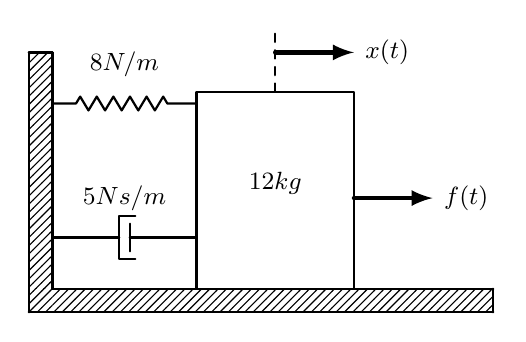
\begin{tikzpicture}
	\tikzstyle{spring}=[thick,decorate,decoration={zigzag,pre length=0.3cm,post length=0.3cm,segment length=6}]
	\tikzstyle{damper}=[thick,decoration={markings,  
	  mark connection node=dmp,
	  mark=at position 0.5 with 
	  {
		\node (dmp) [thick,inner sep=0pt,transform shape,rotate=-90,minimum width=15pt,minimum height=3pt,draw=none] {};
		\draw [thick] ($(dmp.north east)+(2pt,0)$) -- (dmp.south east) -- (dmp.south west) -- ($(dmp.north west)+(2pt,0)$);
		\draw [thick] ($(dmp.north)+(0,-5pt)$) -- ($(dmp.north)+(0,5pt)$);
	  }
	}, decorate]
	\tikzstyle{ground}=[fill,pattern=north east lines,draw=none,minimum width=0.75cm,minimum height=0.3cm,inner sep=0pt,outer sep=0pt]
	
	\node [style={draw,outer sep=0pt,thick}] (M) [minimum width=2cm, minimum height=2.5cm]  {$			\begin{array}{c}
		12 kg\\[5pt]
	\end{array}$};
	\draw [-latex,ultra thick] (M.north) ++(0cm, 0.5cm) -- +(1cm,0cm) node [right,draw=none] (y1) {$x(t)$};
	\draw [dashed] (M.north) -- +(0cm,0.8cm);
	
	\node (ground) [ground,anchor=north,yshift=-0cm,minimum width=5.6cm,xshift=-0.03cm] at (M.south) {};
	\draw (ground.north east) -- (ground.north west);
	\draw (ground.south east) -- (ground.south west);
	\draw (ground.north east) -- (ground.south east);
	
	\node (fill) [ground,xshift=-0.15cm,minimum height = 0.3cm, minimum width = 0.3cm] at (ground.west) {};
	\draw (fill.north west) -- (fill.south west);
	\draw (fill.south west) -- (fill.south east);
	
	
	\node (wall) [ground, rotate=-90, minimum width=3cm,anchor=south east] at (fill.north west) {};
	\draw (wall.north east) -- (wall.north west);
	\draw (wall.north west) -- (wall.south west);
	\draw (wall.south west) -- (wall.south east);
	
	
	\draw [spring] (wall.170) -- ($(M.north west)!(wall.170)!(M.south west)$)node [midway,yshift=6pt, above,draw=none] {$8 N/m $};
	\draw [damper] (wall.10) -- ($(M.north west)!(wall.10)!(M.south west)$)node [midway,yshift=6pt, above,draw=none] {$5 Ns/m $};;
	
	\draw [-latex,ultra thick] (M.east) ++ (0cm,-.10cm) -- +(1cm,0cm) node [right,draw=none] {$f(t)$};
	\end{tikzpicture}
\end{center}
\rule{\textwidth}{1pt}


\noindent\textbf{Given:} As per diagram

\vspace{12pt}
\noindent\textit{\textbf{Solution:}}

\vspace{12pt}

Equation of Motion:\\
\begin{center}
	$M\dfrac{d^2x(t)}{dt^2}+fv\dfrac{dx(t)}{dt}+Kx(t)=f(t)$\\
\end{center}
Substitute the Given:\\
\begin{center}
	$12\dfrac{d^2x(t)}{dt^2}+5\dfrac{dx(t)}{dt}+8x(t)=f(t)$\\
\end{center}
Laplace Transform:\\[12pt]
(Consider that the Initial Condition is $0$)\\
\begin{center}
	$12s^2X(s)+5sX(s)+8x(s)=F(s)$\\
\end{center}
Transfer function $\dfrac{X(s)}{F(s)}$\\
\begin{center}
	\begin{tabular}{|c|}
		\hline \\
		$\dfrac{X(s)}{F(s)}=\dfrac{1}{12s^2+5s+8}$	\\ [12pt]
	\hline
	\end{tabular}	
\end{center}

\clearpage

\rule{\textwidth}{1pt}
\textbf{Problem 27}\\
Find the transfer function $\dfrac{X_2(s)}{F(s)}$\\
\begin{center}
	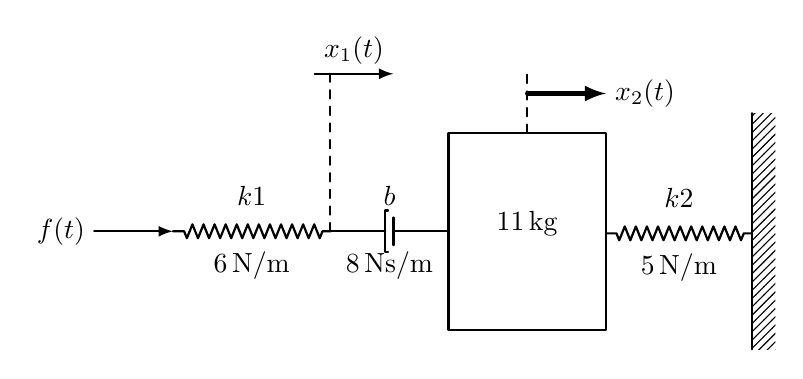
\begin{tikzpicture}[every node/.style={draw,outer sep=0pt,thick}]
		\tikzstyle{spring}=[thick,decorate,decoration={zigzag,pre length=0.1cm,post length=0.1cm,segment length=4}]
		\tikzstyle{damper}=[thick,decoration={markings,
		  mark connection node=dmp,
		  mark=at position 0.5 with
		  {
			\node (dmp) [thick,inner sep=0pt,transform shape,rotate=90,minimum width=15pt,minimum height=3pt,draw=none] {};
			\draw [thick] ($(dmp.north east)+(2pt,0)$) -- (dmp.south east) -- (dmp.south west) -- ($(dmp.north west)+(2pt,0)$);
			\draw [thick] ($(dmp.north)+(0,-5pt)$) -- ($(dmp.north)+(0,5pt)$);
		  }
		}, decorate]
		\tikzstyle{ground}=[fill,pattern=north east lines,draw=none,minimum width=0.75cm,minimum height=0.3cm]
	
		\begin{scope}[xshift=7cm]
			% Mass block
			\node (M) [minimum width=2cm, minimum height=2.5cm, draw, fill=white] {%
				$\begin{array}{c}
					11 \, \mathrm{kg}\\[5pt]
				\end{array}$
			};
	
			% x_2(t) arrow
			\draw [-latex,ultra thick] (M.north) ++(0cm, 0.5cm) -- +(1cm,0cm) node [right,draw=none] {$x_2(t)$};
			\draw [dashed] (M.north) -- +(0cm,0.8cm);
	
			% Wall and spring
			\node (wall) [ground, rotate=90, minimum width=3cm, yshift=-3cm] {};
			\draw (wall.north east) -- (wall.north west);
			\draw [spring] (wall.100) -- ($(M.north east)!(wall.100)!(M.south east)$) 
				node [midway,yshift=6pt, above,draw=none] {$k2$}
				node [midway,yshift=-4pt, below,draw=none] {$5 \, \mathrm{N/m}$};
	
			% Spring before the damper
			\draw [damper] (M.west) -- ++(-1.5cm,0) 
				node [midway,yshift=6pt, above,draw=none] {$b$}
				node [midway,yshift=-4pt, below,draw=none] {$8 \, \mathrm{Ns/m}$};
	
			% Add dashed x_2(t) arrow at damper's left side
			\draw [-latex,thick] ([xshift=-1.7cm,yshift=2cm] M.west) -- ++(1cm,0)
			node [midway,above,draw=none] {$x_1(t)$};
			\draw [dashed] ([xshift=-1.5cm] M.west) -- +(0cm,2cm);

	
			%
			\draw [spring] ([xshift=-1.5cm] M.west) -- ++(-2cm,0) 
				node [midway,yshift=6pt, above,draw=none] {$k1$}
				node [midway,yshift=-4pt, below,draw=none] {$6 \, \mathrm{N/m}$};
	
			% Rightward arrow for F(t)
			\draw [-latex,thick] ([xshift=-4.5cm] M.west) -- ++(1cm,0) 
				node [midway,left,xshift=-.5cm,draw=none] {$f(t)$};
		\end{scope}
	\end{tikzpicture}
\end{center}
\rule{\textwidth}{1pt}


\noindent\textbf{Given:} As per diagram

\vspace{12pt}
\noindent\textit{\textbf{Solution:}}

\vspace{12pt}

Equation for $X_1(t)$:\\
\begin{center}
	$m_1x_1(t)=f(t)-k_1x_1(t)-b[x_1(t)-x_2(t)]$\\
\end{center}
Simplify:\\
\begin{center}
	$11x_1(t)=f(t)-6x_1(t)-8[x_1(t)-x_2(t)]$\\
\end{center}
Equation for $X_2(t)$:\\
\begin{center}
	$m_2x_2(t)=b[x_1(t)-x_2(t)]-k_2x_2(t)$\\
\end{center}
Simplify:\\
\begin{center}
	$11x_2(t)=8[x_1(t)-x_2(t)]-5x_2(t)$\\
\end{center}
Apply the Laplace Transform\\[12pt]
For M1\\
\begin{center}
	$11s^2x_1(s)=f(s)-6x_1(s)-8[sx_1(s)-sx_2(s)]$\\
\end{center}
Simplifying\\
\begin{center}
	$11s^2x_1(s)+8sx_1(s)+6x_1(s)-8sx_2(s)=F(s)$\\
\end{center}
This becomes\\
\begin{center}
	$(11s^2+8s+6)x_1(s)-8sx_2(s)=F(s)$\\
\end{center}
For M2\\
\begin{center}
	$11sx_2(s)=8[sx_1(s)-sx_2(s)]-5x_2(s)$\\
\end{center}
Simplifying\\
\begin{center}
	$11sx_2(s)+8sx_2(s)+5sx_2(s)=8sx_2(s)$\\
\end{center}
This becomes\\
\begin{center}
	$(11s^2+8s+5)x_2(s)=8sx_1(s)$\\
\end{center}
Solve for $x_1(s)$ and $x_1(s)$\\[12pt]
From the second equation for $x_2(s)$\\
\begin{center}
	$x_1(s)=\dfrac{(11s^2+8s+5)}{8s}x_2(s)$\\
\end{center}
Substitute into the first equation\\
\begin{center}
	$(11s^2+8s+5)\dfrac{(11s^2+8s+5)}{8s}x_2(s)-8sx_2(s)=F(s)$\\
\end{center}
Multiply out the terms\\
\begin{center}
	$\dfrac{(11s^2+8s+5)(11s^2+8s+5)}{8s}x_2(s)-8sx_2(s)=F(s)$\\
\end{center}
Simplify the expression\\
\begin{center}
	$x_2(s)\left[\dfrac{(11s^2+8s+5)(11s^2+8s+5)}{8s}-8s\right]=F(s) $\\
\end{center}
Thus, the Transfer Function is\\
\begin{center}
	\begin{tabular}{|c|}
		\hline \\
		$G(s)=\dfrac{X_2(s)}{F(s)}=\dfrac{8s}{(11s^2+8s+5)(11s^2+8s+5)-64s^2}$	\\ [12pt]
	\hline
	\end{tabular}	
\end{center}

\clearpage

\rule{\textwidth}{1pt}
\textbf{Problem 28}\\
Find the transfer function $\dfrac{X_2(s)}{F(s)}$\\

\begin{center}
	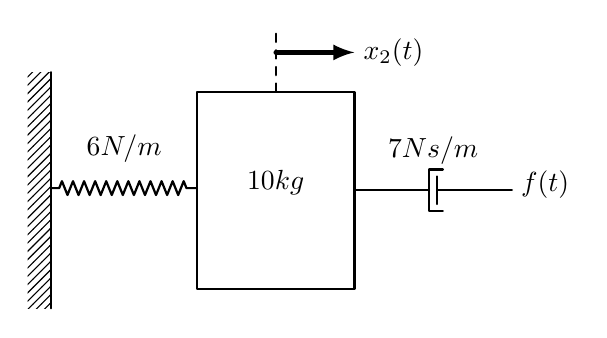
\begin{tikzpicture}[every node/.style={draw,outer sep=0pt,thick}]
		\tikzstyle{spring}=[thick,decorate,decoration={zigzag,pre length=0.1cm,post length=0.1cm,segment length=4}]
		\tikzstyle{damper}=[thick,decoration={markings,
		  mark connection node=dmp,
		  mark=at position 0.5 with
		  {
			\node (dmp) [thick,inner sep=0pt,transform shape,rotate=-90,minimum width=15pt,minimum height=3pt,draw=none] {};
			\draw [thick] ($(dmp.north east)+(2pt,0)$) -- (dmp.south east) -- (dmp.south west) -- ($(dmp.north west)+(2pt,0)$);
			\draw [thick] ($(dmp.north)+(0,-5pt)$) -- ($(dmp.north)+(0,5pt)$);
		  }
		}, decorate]
		\tikzstyle{ground}=[fill,pattern=north east lines,draw=none,minimum width=0.75cm,minimum height=0.3cm]
	
		\begin{scope}[xshift=7cm]
			\node (M) [minimum width=2cm, minimum height=2.5cm, draw, fill=white] {$			\begin{array}{c}
				10 kg\\[5pt]
				
			\end{array}$};

			\draw [-latex,ultra thick] (M.north) ++(0cm, 0.5cm) -- +(1cm,0cm) node [right,draw=none] (y1) {$x_2(t)$};
			\draw [dashed] (M.north) -- +(0cm,0.8cm);
	

		\node (wall) [ground, rotate=-90, minimum width=3cm,yshift=-3cm] {};
		\draw (wall.north east) -- (wall.north west);
	
	
		\draw [spring] (wall.100) -- ($(M.north west)!(wall.100)!(M.south west)$) node [midway,yshift=6pt, above,draw=none] {$6 N/m$};
	
		\draw [damper] (M.east) ++ (0,0) -- +(2cm,0) node [midway,yshift=6pt, above,draw=none] {$7 Ns/m$} node[right,yshift=2pt, draw=none] {$f(t)$};
		\end{scope}
	\end{tikzpicture}
	\end{center}

	\rule{\textwidth}{1pt}

\noindent\textbf{Given:} As per diagram

\vspace{12pt}
\noindent\textit{\textbf{Solution:}}

\vspace{12pt}

Formulate the Equation of Motion\\
\begin{center}
	$mx_2(t)+cx_2(t)+kx_2(t)=f(t)$\\
\end{center}
Substitute the Values\\
\begin{center}
	$10x_2(t)+7x_2(t)+6x_2(t)=f(t)$\\
\end{center}
Take the Laplace Transform\\
\begin{center}
	$10s^2x_2(s)+7sx_2(s)+6x_2(s)=f(s)$\\
\end{center}
Solve for $\dfrac{X_2(s)}{F(s)}$\\[12pt]
Rearrange the Equation\\
\begin{center}
	$x_2(s)(10s^2+7s+6)=F(s)$\\
\end{center}
Transfer Function:\\
\begin{center}
	\begin{tabular}{|c|}
		\hline \\
		$G(s)=\dfrac{X_2(s)}{F(s)}=\dfrac{1}{10s^2+7s+6}$	\\ [12pt]
	\hline
	\end{tabular}	
\end{center}

\clearpage

\rule{\textwidth}{1pt}
\textbf{Problem 29}\\
Find the transfer function $G(s)=\dfrac{X_2(s)}{F(s)}$\\

\begin{center}
	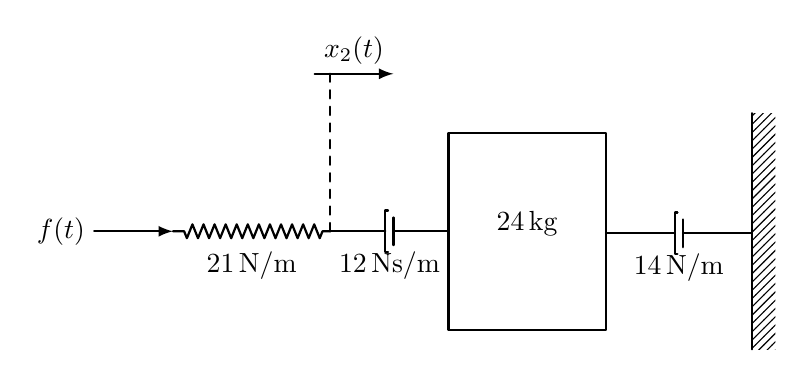
\begin{tikzpicture}[every node/.style={draw,outer sep=0pt,thick}]
		\tikzstyle{spring}=[thick,decorate,decoration={zigzag,pre length=0.1cm,post length=0.1cm,segment length=4}]
		\tikzstyle{damper}=[thick,decoration={markings,
		  mark connection node=dmp,
		  mark=at position 0.5 with
		  {
			\node (dmp) [thick,inner sep=0pt,transform shape,rotate=90,minimum width=15pt,minimum height=3pt,draw=none] {};
			\draw [thick] ($(dmp.north east)+(2pt,0)$) -- (dmp.south east) -- (dmp.south west) -- ($(dmp.north west)+(2pt,0)$);
			\draw [thick] ($(dmp.north)+(0,-5pt)$) -- ($(dmp.north)+(0,5pt)$);
		  }
		}, decorate]
		\tikzstyle{ground}=[fill,pattern=north east lines,draw=none,minimum width=0.75cm,minimum height=0.3cm]
	
		\begin{scope}[xshift=7cm]
			% Mass block
			\node (M) [minimum width=2cm, minimum height=2.5cm, draw, fill=white] {%
				$\begin{array}{c}
					24 \, \mathrm{kg}\\[5pt]
				\end{array}$
			};
	
			% Wall and spring
			\node (wall) [ground, rotate=90, minimum width=3cm, yshift=-3cm] {};
			\draw (wall.north east) -- (wall.north west);
			\draw [damper] (wall.100) -- ($(M.north east)!(wall.100)!(M.south east)$) 
				node [midway,yshift=-4pt, below,draw=none] {$14 \, \mathrm{N/m}$};
	
			% Spring before the damper
			\draw [damper] (M.west) -- ++(-1.5cm,0) 
				node [midway,yshift=-4pt, below,draw=none] {$12 \, \mathrm{Ns/m}$};
	
			% Add dashed x_2(t) arrow at damper's left side
			\draw [-latex,thick] ([xshift=-1.7cm,yshift=2cm] M.west) -- ++(1cm,0)
			node [midway,above,draw=none] {$x_2(t)$};
			\draw [dashed] ([xshift=-1.5cm] M.west) -- +(0cm,2cm);

	
			%
			\draw [spring] ([xshift=-1.5cm] M.west) -- ++(-2cm,0) 
				node [midway,yshift=-4pt, below,draw=none] {$21 \, \mathrm{N/m}$};
	
			% Rightward arrow for F(t)
			\draw [-latex,thick] ([xshift=-4.5cm] M.west) -- ++(1cm,0) 
				node [midway,left,xshift=-.5cm,draw=none] {$f(t)$};
		\end{scope}
	\end{tikzpicture}
\end{center}

	\rule{\textwidth}{1pt}

\noindent\textbf{Given:} As per diagram

\vspace{12pt}
\noindent\textit{\textbf{Solution:}}

\vspace{12pt}

Formulate the Equation of Motion\\
\begin{center}
	$mx_2(t)=f(t)-c_1x_2(t)-kx_2(t)-c_2x_2(t)$\\
\end{center}
Simplify the Equation\\
\begin{center}
	$mx_2(t)+(c_1+c_2)x_2(t)+kx_2(t)=f(t)$\\
\end{center}
Substitute the Values\\
\begin{center}
	$24x_2(t)+(12+4)x_2(t)+21x_2(t)=f(t)$\\
\end{center}
Simplify\\
\begin{center}
	$24x_2(t)+26x_2(t)+21x_2(t)=f(t)$\\
\end{center}
Take the Laplace Transform\\
\begin{center}
	$24s^2x_2(s)+26sx_2(s)+21x_2(s)=f(s)$\\
\end{center}
Solve for $\dfrac{X_2(s)}{F(s)}$\\[12pt]
Rearrange the Equation\\
\begin{center}
	$x_2(s)(24s^2+26s+21)=F(s)$\\
\end{center}
Transfer Function:\\
\begin{center}
	\begin{tabular}{|c|}
		\hline \\
		$G(s)=\dfrac{X_2(s)}{F(s)}=\dfrac{1}{24s^2+26s+21}$	\\ [12pt]
	\hline
	\end{tabular}	
\end{center}

\clearpage

\rule{\textwidth}{1pt}
\textbf{Problem 30}\\
Find the transfer function $G(s)=\dfrac{X_2(s)}{F(s)}$\\

\begin{center}
	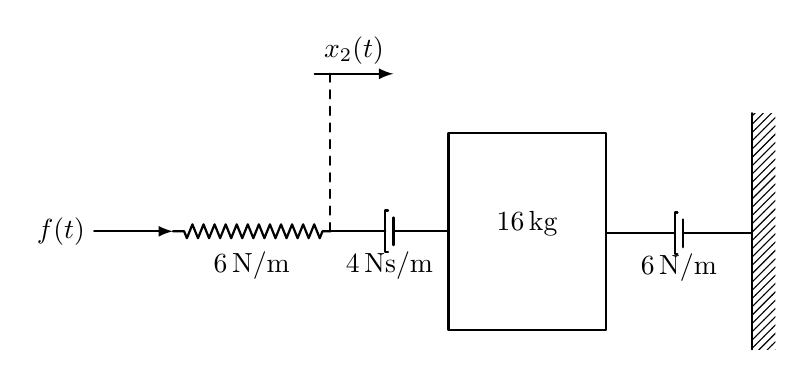
\begin{tikzpicture}[every node/.style={draw,outer sep=0pt,thick}]
		\tikzstyle{spring}=[thick,decorate,decoration={zigzag,pre length=0.1cm,post length=0.1cm,segment length=4}]
		\tikzstyle{damper}=[thick,decoration={markings,
		  mark connection node=dmp,
		  mark=at position 0.5 with
		  {
			\node (dmp) [thick,inner sep=0pt,transform shape,rotate=90,minimum width=15pt,minimum height=3pt,draw=none] {};
			\draw [thick] ($(dmp.north east)+(2pt,0)$) -- (dmp.south east) -- (dmp.south west) -- ($(dmp.north west)+(2pt,0)$);
			\draw [thick] ($(dmp.north)+(0,-5pt)$) -- ($(dmp.north)+(0,5pt)$);
		  }
		}, decorate]
		\tikzstyle{ground}=[fill,pattern=north east lines,draw=none,minimum width=0.75cm,minimum height=0.3cm]
	
		\begin{scope}[xshift=7cm]
			% Mass block
			\node (M) [minimum width=2cm, minimum height=2.5cm, draw, fill=white] {%
				$\begin{array}{c}
					16 \, \mathrm{kg}\\[5pt]
				\end{array}$
			};
	
			% Wall and spring
			\node (wall) [ground, rotate=90, minimum width=3cm, yshift=-3cm] {};
			\draw (wall.north east) -- (wall.north west);
			\draw [damper] (wall.100) -- ($(M.north east)!(wall.100)!(M.south east)$) 
				node [midway,yshift=-4pt, below,draw=none] {$6 \, \mathrm{N/m}$};
	
			% Spring before the damper
			\draw [damper] (M.west) -- ++(-1.5cm,0) 
				node [midway,yshift=-4pt, below,draw=none] {$4 \, \mathrm{Ns/m}$};
	
			% Add dashed x_2(t) arrow at damper's left side
			\draw [-latex,thick] ([xshift=-1.7cm,yshift=2cm] M.west) -- ++(1cm,0)
			node [midway,above,draw=none] {$x_2(t)$};
			\draw [dashed] ([xshift=-1.5cm] M.west) -- +(0cm,2cm);

	
			%
			\draw [spring] ([xshift=-1.5cm] M.west) -- ++(-2cm,0) 
				node [midway,yshift=-4pt, below,draw=none] {$6 \, \mathrm{N/m}$};
	
			% Rightward arrow for F(t)
			\draw [-latex,thick] ([xshift=-4.5cm] M.west) -- ++(1cm,0) 
				node [midway,left,xshift=-.5cm,draw=none] {$f(t)$};
		\end{scope}
	\end{tikzpicture}
\end{center}

	\rule{\textwidth}{1pt}

\noindent\textbf{Given:} As per diagram

\vspace{12pt}
\noindent\textit{\textbf{Solution:}}

\vspace{12pt}

Formulate the Equation of Motion\\
\begin{center}
	$mx_2(t)=f(t)-c_1x_2(t)-kx_2(t)-c_2x_2(t)$\\
\end{center}
Simplify the Equation\\
\begin{center}
	$mx_2(t)+(c_1+c_2)x_2(t)+kx_2(t)=f(t)$\\
\end{center}
Substitute the Values\\
\begin{center}
	$16x_2(t)+(4+6)x_2(t)+6x_2(t)=f(t)$\\
\end{center}
Simplify\\
\begin{center}
	$16x_2(t)+10x_2(t)+6x_2(t)=f(t)$\\
\end{center}
Take the Laplace Transform\\
\begin{center}
	$16s^2x_2(s)+10sx_2(s)+6x_2(s)=f(s)$\\
\end{center}
Solve for $\dfrac{X_2(s)}{F(s)}$\\[12pt]
Rearrange the Equation\\
\begin{center}
	$x_2(s)(16s^2+10s+6)=F(s)$\\
\end{center}
Transfer Function:\\
\begin{center}
	\begin{tabular}{|c|}
		\hline \\
		$G(s)=\dfrac{X_2(s)}{F(s)}=\dfrac{1}{16s^2+10s+6}$	\\ [12pt]
	\hline
	\end{tabular}	
\end{center}

\clearpage

\rule{\textwidth}{1pt}
\textbf{Problem 31}\\
Find the transfer function $G(s)=\dfrac{X_1(s)}{F(s)}$\\

\begin{center}
	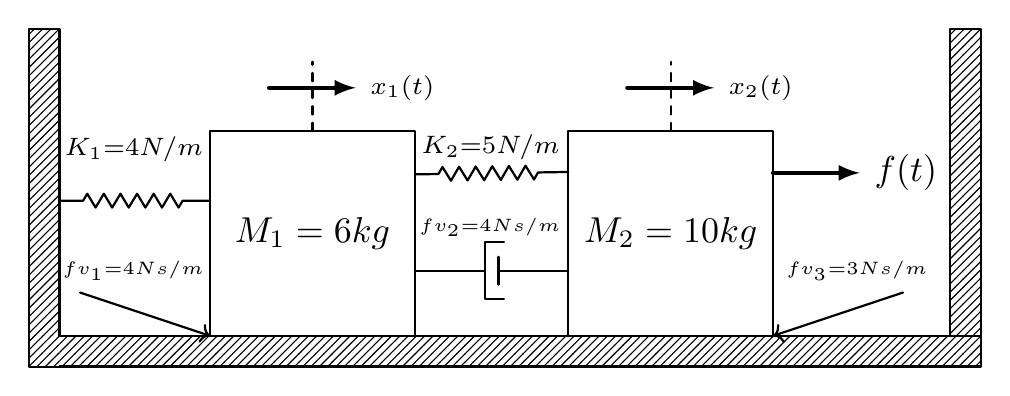
\begin{tikzpicture}[scale=1.1, every node/.style={scale=1.3}]
		\tikzstyle{spring}=[thick,decorate,decoration={zigzag,pre length=0.3cm,post length=0.3cm,segment length=6}]
		\tikzstyle{damper}=[thick,decoration={markings,  
			mark connection node=dmp,
			mark=at position 0.5 with 
			{
				\node (dmp) [thick,inner sep=0pt,transform shape,rotate=-90,minimum width=15pt,minimum height=3pt,draw=none] {};
				\draw [thick] ($(dmp.north east)+(2pt,0)$) -- (dmp.south east) -- (dmp.south west) -- ($(dmp.north west)+(2pt,0)$);
				\draw [thick] ($(dmp.north)+(0,-5pt)$) -- ($(dmp.north)+(0,5pt)$);
			}
		}, decorate]
		\tikzstyle{ground}=[fill,pattern=north east lines,draw=none,minimum width=0.75cm,minimum height=0.3cm,inner sep=0pt,outer sep=0pt]
	
		\node [draw, outer sep=0pt, thick] (M) [minimum width=2cm, minimum height=2cm] {$M_1=6 kg$};
		\node [draw, outer sep=0pt, thick] (M2) [minimum width=2cm, minimum height=2cm, xshift = 3.5cm] {$M_2=10 kg$};
	
		\node (ground) [ground,anchor=north,yshift=-0.0cm,minimum width=9cm,xshift=2.03cm] at (M.south) {};
		\draw (ground.north west) -- (ground.north east) -- (ground.south east) -- (ground.south west);
	
		\node (fill) [ground,xshift=-0.15cm,minimum height = 0.3cm, minimum width = 0.3cm] at (ground.west) {};
		\draw (fill.north west) -- (fill.south west) -- (fill.south east);
	
		\draw [spring] (M.30) -- (M2.-211) node (k) [midway,above] {$_{K_2=5N/m}$};
		\draw [damper] (M.-20) -- (M2.-160) node (k) [midway,above,yshift=0.2cm] {$_{_{f{v_2}=4Ns/m}}$};
	
		\node (wall) [ground, rotate=-90, minimum width=3cm,anchor=south east] at (fill.north west) {};
		\draw (wall.north east) -- (wall.north west) -- (wall.south west) -- (wall.south east);
	
		\node (wall2) [ground, rotate=-90, minimum width=3cm,anchor=north east,yshift=9cm] at (fill.north east) {};
		\draw (wall2.north east) -- (wall2.north west) -- (wall2.south west) -- (wall2.south east);
	
		\draw [->, thick] 
    ($(M.south west) + (-1.5cm, 0.5cm)$) -- ($(M.south west) + (0cm, 0cm)$)
    node [midway,above,yshift=0.2cm,xshift=-0.1cm] {$_{_{f{v_1}=4Ns/m}}$};

	\draw [->, thick] 
    ($(M2.south east) + (1.5cm, 0.5cm)$) -- ($(M2.south east) + (0cm, 0cm)$)
	node [midway,above,yshift=0.2cm,xshift=0.2cm] {$_{_{f{v_3}=3Ns/m}}$};

	
		\draw [spring] (wall.40) -- ($(M.north west)!(wall.40)!(M.south west)$) node [midway,yshift=0.5cm] {$_{K_1=4N/m}$};
		
		\draw [-latex,ultra thick] (M.north) ++(-0.5cm, 0.5cm) -- +(1cm,0cm) node [right,draw=none] (y1) {$_{x_1(t)}$};
		\draw [dashed] (M.north) -- +(0cm,0.8cm);
	
		\draw [-latex,ultra thick] (M2.north) ++(-0.5cm, 0.5cm) -- +(1cm,0cm) node [right,draw=none] (y1) {$_{x_2(t)}$};
		\draw [dashed](M2.north) -- +(0cm,0.8cm);;

		\draw [-latex,ultra thick] (M2.east) ++(0cm, 0.7cm) -- +(1cm,0cm) node [right,draw=none] (y1) {$f(t)$};
	
		
	\end{tikzpicture}
	\end{center}
	

\rule{\textwidth}{1pt}

\noindent\textbf{Given:} As per diagram

\vspace{12pt}
\noindent\textit{\textbf{Solution:}}

\vspace{12pt}

Derive the Equations of Motion:\\[12pt]
Equation of Motion for M1:\\
\begin{center}
	$M_1\ddot{x}_1(t)=-f_{v1}\dot{x}_1(t)-k_1x_1(t)+f_{v2}[\dot{x}_2(t)-\dot{x}_1(t)]+k_2[x_2(t)-x_1(t)]$\\
\end{center}
Substitute the Values:\\
\begin{center}
	$6\ddot{x}_1(t)=-4\dot{x}_1(t)-4x_1(t)+4[\dot{x}_2(t)-\dot{x}_1(t)]+5[x_2(t)-x_1(t)]$\\
\end{center}
Simplifying:\\
\begin{center}
	$6\ddot{x}_1(t)=-(4+5)x_1(t)+5x_2(t)-(4+4)\dot{x}_1(t)+4\dot{x}_2(t)$\\[12pt]
	$6\ddot{x}_1(t)=-9x_1(t)+5x_2(t)-8\dot{x}_1(t)+4\dot{x}_2(t)$\\[12pt]
\end{center}
Equation of Motion for M2:\\
\begin{center}
	$M_2\ddot{x}_2(t)=k_2[x_1(t)-x_2(t)]+f_{v2}[\dot{x}_1(t)-\dot{x}_2(t)]-f_{v3}\dot{x}_2(t)+F(t)$\\
\end{center}
Substituting the Given Values:\\
\begin{center}
	$10\ddot{x}_2(t)=5[x_1(t)-x_2(t)]+4[\dot{x}_1(t)-\dot{x}_2(t)]-3\dot{x}_2(t)+F(t)$\\
\end{center}
Simplifying:\\
\begin{center}
	$10\ddot{x}_2(t)=5x_1(t)-5x_2(t)+4\dot{x}_1(t)-(4+3)\dot{x}_2(t)+F(t)$\\[12pt]
	$10\ddot{x}_2(t)=5x_1(t)-5x_2(t)+4\dot{x}_1(t)-7\dot{x}_2(t)+F(t)$\\
\end{center}
Laplace Transform:\\[12pt]
For M1:\\
\begin{center}
	$6s^2X_1(s)=-9X_1(s)+5X_2(s)-8sX_1(s)+4sX_2(s)$\\[12pt]
\end{center}
Simplifying:\\
\begin{center}
	$(6s^2+8s+9)X_1(s)=(5+4s)X_2(s)$\\
\end{center}
For M2:\\
\begin{center}
	$10s^2X_2(s)=5X_1(s)-5X_2(s)+4sX_1(s)-7sX_2(s)+F(s)$\\
\end{center}
Simplifying:\\
\begin{center}
	$(10s^2+7s+5)X_2(s)=(5+4s)X_1(s)+F(s)$\\
\end{center}
Solving for the Transfer Function:\\[12pt]
Substitute $X_2(s)$ from the Second Equation into the First Equation:\\
\begin{center}
	$(6s^2+8s+9)X_1(s)=(5+4s)\left[\dfrac{(5+4s)X_1(s)+F(s)}{10s^2+7s+5}\right] $\\
\end{center}
Final Transfer Function:\\
\begin{center}
	\begin{tabular}{|c|}
		\hline \\
		$\dfrac{X_1(s)}{F(s)}=\dfrac{5+4s}{(6s^2+8s+9)(10s^2+7s+5)-(5+4s)^2}$	\\ [12pt]
	\hline
	\end{tabular}	
\end{center}

\clearpage


\rule{\textwidth}{1pt}
\textbf{Problem 32}\\
Find the transfer function $G(s)=\dfrac{X_2(s)}{F(s)}$\\
\begin{center}
	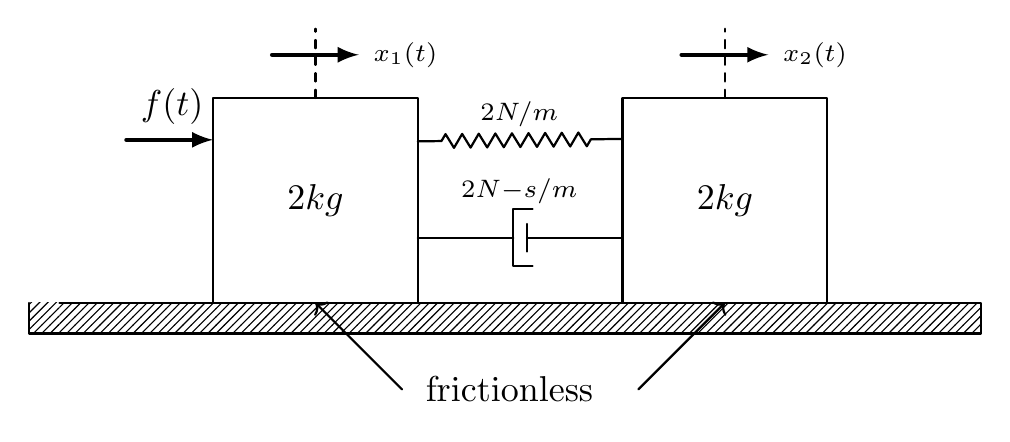
\begin{tikzpicture}[scale=1.1, every node/.style={scale=1.3}]
		\tikzstyle{spring}=[thick,decorate,decoration={zigzag,pre length=0.3cm,post length=0.3cm,segment length=6}]
		\tikzstyle{damper}=[thick,decoration={markings,  
			mark connection node=dmp,
			mark=at position 0.5 with 
			{
				\node (dmp) [thick,inner sep=0pt,transform shape,rotate=-90,minimum width=15pt,minimum height=3pt,draw=none] {};
				\draw [thick] ($(dmp.north east)+(2pt,0)$) -- (dmp.south east) -- (dmp.south west) -- ($(dmp.north west)+(2pt,0)$);
				\draw [thick] ($(dmp.north)+(0,-5pt)$) -- ($(dmp.north)+(0,5pt)$);
			}
		}, decorate]
		\tikzstyle{ground}=[fill,pattern=north east lines,draw=none,minimum width=0.75cm,minimum height=0.3cm,inner sep=0pt,outer sep=0pt]
	
		\node [draw, outer sep=0pt, thick] (M) [minimum width=2cm, minimum height=2cm] {$2 kg$};
		\node [draw, outer sep=0pt, thick] (M2) [minimum width=2cm, minimum height=2cm, xshift = 4cm] {$2 kg$};
	
		\node (ground) [ground,anchor=north,yshift=-0.0cm,minimum width=9cm,xshift=2.cm] at (M.south) {};
		\draw (ground.north west) -- (ground.north east) -- (ground.south east) -- (ground.south west);
	
		\node (fill) [ground,xshift=-0.15cm,minimum height = 0.3cm, minimum width = 0.3cm] at (ground.west) {};
		\draw (fill.north west) -- (fill.south west) -- (fill.south east);
	
		\draw [spring] (M.30) -- (M2.-211) node (k) [midway,above] {$_{2 N/m} $};
		\draw [damper] (M.-20) -- (M2.-160) node (k) [midway,above,yshift=0.2cm] {$_{2 N-s/m}$};
	
		% Removed wall and wall2 elements
	
		\draw [-latex,ultra thick] (M.north) ++(-0.5cm, 0.5cm) -- +(1cm,0cm) node [right,draw=none] (y1) {$_{x_1(t)}$};
		\draw [dashed] (M.north) -- +(0cm,0.8cm);
	
		\draw [-latex,ultra thick] (M2.north) ++(-0.5cm, 0.5cm) -- +(1cm,0cm) node [right,draw=none] (y1) {$_{x_2(t)}$};
		\draw [dashed](M2.north) -- +(0cm,0.8cm);;

		\draw [-latex,ultra thick] (M.west) ++(-1cm, 0.7cm) -- +(1cm,0cm) node [above,draw=none,xshift=-0.4cm] (y1) {$f(t)$};
		
		% Add frictionless arrows focused on M and M2
		\draw[<-,thick] (M.south) -- +(1,-1cm) node[below,right,xshift=0.1cm] {frictionless};
		\draw[<-,thick] (M2.south) -- +(-1cm,-1cm);
	
	\end{tikzpicture}
\end{center}

\rule{\textwidth}{1pt}

\noindent\textbf{Given:} As per diagram

\vspace{12pt}
\noindent\textit{\textbf{Solution:}}

\vspace{12pt}

Equation for Mass 1:\\[12pt]
Using Newton's second law:\\
\begin{center}
	$M_1\ddot{x}_1(t)=f(t)-B[\dot{x}_1(t)-\dot{x}_2(t)]-K[x_1(t)-x_2(t)]$\\
\end{center}
Taking the Laplace Transform (with zero initial conditions):\\
\begin{center}
	$M_1s^2X_1(s)=F(s)-Bs[X_1(s)-X_2(s)]-K[X_1(s)-X_2(s)]$\\
\end{center}
Substitute the Values:\\
\begin{center}
	$2s^2X_1(s)=F(s)-2s[X_1(s)-X_2(s)]-2[X_1(s)-X_2(s)]$\\[12pt]
	$2s^2X_1(s)=F(s)-(2s+2)[X_1(s)-X_2(s)]$\\[12pt]
\end{center}
Equation for Mass 2:\\[12pt]
Using Newton's second law:\\
\begin{center}
	$M_2\ddot{x}_2(t)=B[\dot{x}_1(t)-\dot{x}_2(t)]-K[x_1(t)-x_2(t)]$\\
\end{center}
Taking the Laplace Transform (with zero initial conditions):\\
\begin{center}
	$M_2s^2X_2(s)=Bs[X_1(s)-X_2(s)]-K[X_1(s)-X_2(s)]$\\
\end{center}
Substitute the Values:\\
\begin{center}
	$2s^2X_2(s)=2s[X_1(s)-X_2(s)]+2[X_1(s)-X_2(s)]$\\[12pt]
	$2s^2X_2(s)=(2s+2)[X_1(s)-X_2(s)]$\\[12pt]
\end{center}
Solve the System of Equations:\\
\begin{center}
	$X_1(s)-X_2(s)=\dfrac{2s^2X_2(s)}{2s+2}$\\[12pt]
	$X_1(s)=X_2(s)+\dfrac{s^2X_2(s)}{s+1}$\\[12pt]
	$X_1(s)=\dfrac{X_2(s)(s^2+s+1)}{s+1}$\\[12pt]
\end{center}
Substitute into the First Equation:\\[12pt]
Substitute this Expression for $X_1(s)$ into the First Equation:\\
\begin{center}
	$2s^2\dfrac{X_2(s)(s^2+s+1)}{s+1}=F(s)-(2s+2)\left[\dfrac{X_2(s)(s^2+s+1)}{s+1}-X_2(s)\right] $\\[12pt]
\end{center}
Final Transfer Function:\\
\begin{center}
	\begin{tabular}{|c|}
		\hline \\
		$G(s)=\dfrac{s+1}{2s^4+4s^3+4s^2+2s}$	\\ [12pt]
	\hline
	\end{tabular}	
\end{center}

\clearpage

\rule{\textwidth}{1pt}
\textbf{Problem 33}\\
Find the transfer function $G(s)=\dfrac{X_2(s)}{F(s)}$ for the translational mechanical system shown in the figure\\
\begin{center}
	\begin{tikzpicture}[scale=1.1, every node/.style={scale=1.3}, line cap=round, line join=round, >=stealth]

		% U-shaped structure rotated by -90 degrees
		\begin{scope}[rotate=-90,xshift=-1.35cm,yshift=-0.5cm]
			% Adjusted U-shape dimensions (smaller opening)
			\draw[line width=2mm] (0,5) -- (0,0); % Left vertical line (lengthened to 4 units)
			\draw[line width=2mm] (0,5) -- (2.5,5); % Top horizontal line (shortened to 2.5 units)
			\draw[line width=2mm] (2.5,5) -- (2.5,0); % Right vertical line (lengthened to 4 units)
		\end{scope}

		% Mechanical system diagram
		\tikzstyle{spring}=[thick,decorate,decoration={zigzag,pre length=0.3cm,post length=0.3cm,segment length=6}]
		\tikzstyle{damper}=[thick,decoration={markings,  
			mark connection node=dmp,
			mark=at position 0.5 with 
			{
				\node (dmp) [thick,inner sep=0pt,transform shape,rotate=-90,minimum width=15pt,minimum height=3pt,draw=none] {};
				\draw [thick] ($(dmp.north east)+(2pt,0)$) -- (dmp.south east) -- (dmp.south west) -- ($(dmp.north west)+(2pt,0)$);
				\draw [thick] ($(dmp.north)+(0,-5pt)$) -- ($(dmp.north)+(0,5pt)$);
			}
		}, decorate]
		\tikzstyle{ground}=[fill,pattern=north east lines,draw=none,minimum width=0.75cm,minimum height=0.3cm,inner sep=0pt,outer sep=0pt]
		
		\node [draw, outer sep=0pt, thick] (M2) [minimum width=2cm, minimum height=2.1cm, xshift = 1cm] {$M_1=2 kg$};
		
		\node (ground) [ground,anchor=north,yshift=-0.0cm,minimum width=9cm,xshift=2.cm] at (M.south) {};
		\draw (ground.north west) -- (ground.north east) -- (ground.south east) -- (ground.south west);
		
		\node (fill) [ground,xshift=-0.15cm,minimum height = 0.3cm, minimum width = 0.3cm] at (ground.west) {};
		\draw (fill.north west) -- (fill.south west) -- (fill.south east);
	
		\draw [-latex,ultra thick] (M2.north) ++(-0.5cm, 0.5cm) -- +(1cm,0cm) node [right,draw=none] (y1) {$_{x_1(t)}$};
		\draw [dashed](M2.north) -- +(0cm,0.8cm); % Dashed line for x_1(t)

		\draw [-latex,ultra thick] (M2.north) ++(2cm, 0.5cm) -- +(1cm,0cm) node [right,draw=none] (y1) {$_{x_2(t)}$};
		\draw [dashed](M2.north) ++(2.4cm, 0.2cm) -- +(0cm,0.8cm); % Dashed line for x_2(t)

		\draw [-latex,ultra thick] (M2.west) ++(-1cm, 0.10cm) -- +(1cm,0cm) node [left,draw=none,xshift=-0.8cm] (y1) {$_{f(t)}$};

		\draw [->, thick] 
		($(M2.south west) + (-1.5cm, 0.5cm)$) -- ($(M2.south west) + (0cm, 0.2cm)$)
		node [midway,above,yshift=0.1cm,xshift=-0.2cm] {$_{_{f{v_1}=2Ns/m}}$};

		\draw [->, thick] 
		($(M2.north west) + (-1.5cm, -0.5cm)$) -- ($(M2.north west) + (0cm, 0cm)$)
		node [midway,above,yshift=0.1cm,xshift=-0.8cm] {$_{_{f{v_2}=2N-s/m}}$};

		\draw [<-,ultra thick] (M2.east) ++(2.2cm, 0.8cm) -- +(1cm,0cm) node [right,draw=none] (y1) {$_{M_2=2kg}$};

		\draw [->, thick] 
		($(M2.south east) + (3.5cm, 0.6cm)$) -- ($(M2.south east) + (2.2cm, 0.1cm)$)
		node [midway,above,yshift=0.2cm,xshift=0.5cm] {$_{_{f{v_4}=2N-s/m}}$};
		
		\draw [spring] (M2.east) ++(0cm, 0.6cm) -- +(2.1cm,0cm) node [above,draw=none,xshift=-0.9cm] (y1) {$_{K=2N/m}$};

		\draw [damper] (M2.east) ++(0cm, -0.6cm) -- +(2.1cm,0cm) node [above,draw=none,xshift=-0.9cm,yshift=0.2cm] (y1) {$_{_{f{v_3}=2N-s/m}}$};

	\end{tikzpicture}
\end{center}


\rule{\textwidth}{1pt}

\noindent\textbf{Given:} As per diagram

\vspace{12pt}
\noindent\textit{\textbf{Solution:}}

\vspace{12pt}

Equations of motion for each mass in the Laplace Domain:\\[12pt]
For $M_1$:\\[12pt]
\begin{center}
	$M_1\ddot{x}_1(t)=F(t)-f_{v1}\dot{x}_1(t)-f_{v2}[\dot{x}_1(t)-\dot{x}_2(t)]-K[x_1(t)-x_2(t)]$\\
\end{center}
In Laplace Domain:\\
\begin{center}
	$M_1s^2X_1(s)=F(s)-f_{v1}sX_1(s)-f_{v2}[X_1(s)-X_2(s)]-K[X_1(s)-X_2(s)]$\\
\end{center}
Substitute the values:\\
\begin{center}
	$2s^2X_1(s)=F(s)-2sX_1(s)-2s[X_1(s)-X_2(s)]-2[X_1(s)-X_2(s)]$\\
\end{center}
Simplify the terms:\\
\begin{center}
	$2s^2X_1(s)=F(s)-4sX_1(s)+2sX_2(s)-2X_1(s)+2X_2(s)$\\[12pt]
	$2s^2X_1(s)=F(s)-(2s+2)X_1(s)+(2s+2)X_2(s)$\\[12pt]
\end{center}
Rearrange to:\\
\begin{center}
	$(2s^2+2s+2)X_1(s)-(2s+2)X_2(s)=F(s)$\\
\end{center}
For $M_2$:\\[12pt]
\begin{center}
	$M_2\ddot{x}_2(t)=-f_{v3}\dot{x}_2(t)+f_{v2}[\dot{x}_1(t)-\dot{x}_2(t)]+K[x_1(t)-x_2(t)]$\\
\end{center}
In Laplace Domain:\\
\begin{center}
	$M_2sX_2(s)=-f_{v3}sX_2(s)+f_{v2}[X_1(s)-X_2(s)]+K[X_1(s)-X_2(s)]$\\
\end{center}
Substitute the terms:\\
\begin{center}
	$2s^2X_2(s)=-2sX_2(s)+2s[X_1(s)-sX_2(s)]+2[X_1(s)-X_2(s)]$\\
\end{center}
Simplify the terms:\\
\begin{center}
	$2s^2X_2(s)=-2sX_2(s)+2sX_1(s)-2sX_2(s)+2X_1(s)-2X_2(s)$\\[12pt]
	$2s^2X_2(s)=2sX_1(s)+2X_1(s)-(2s+2)X_2(s)$\\[12pt]
\end{center}
Rearrange to:\\
\begin{center}
	$(2s^2+2s+2)X_2(s)=(2s+2)X_1(s)$\\
\end{center}
Solving the System of Equations\\[12pt]
Solve equation $(2)$ for $X_1(s)$:\\
\begin{center}
	$X_1(s)=\dfrac{(2s^2+2s+2)X_2(s)}{2s+2}$\\
\end{center}
Substitute this into equation $(1)$:\\
\begin{center}
	$(2s^2+2s+2)\left[\dfrac{(2s^2+2s+2)X_2(s)}{2s+2}\right]-(2s+2)X_2(s)=F(s)$\\
\end{center}
Multiply out:\\
\begin{center}
	$\dfrac{(2s^2+2s+2)^2X_2(s)}{2s+2}-(2s+2)X_2(s)=F(s)$\\
\end{center}
Multiply both sides by $2s + 2$ to eliminate the denominator:\\
\begin{center}
	$(2s^2+2s+2)^2X_2(s)-(2s+2)^2X_2(s)=(2s+2)F(s)$\\
\end{center}
Factor out $X_2(s)$ on the left-hand side:\\
\begin{center}
	$[(2s^2+2s+2)^2-(2s+2)^2]X_2(s)=(2s+2)F(s)$\\
\end{center}
Simplify the terms:\\
\begin{center}
	$(2s^2+2s+2)^2=4s^4+8s^3+12s^2+8s+4$\\[12pt]
	$(2s+2)^2=4s^2+8s+4$\\
\end{center}
Subtract the two:\\
\begin{center}
	$(4s^4+8s^3+12s^2+8s+4)-(4s^2+8s+4)=4s^4+8s^3+8s^2$\\
\end{center}
So:\\
\begin{center}
	$(4s^4+8s^3+8s^2)X_2(s)=(2s+2)F(s)$\\
\end{center}
Final Transfer Function:\\
\begin{center}
	\begin{tabular}{|c|}
		\hline \\
		$G(s)=\dfrac{2s+2}{4s^4+8s^3+8s^2}$	\\ [12pt]
	\hline
	\end{tabular}	
\end{center}

\clearpage

\rule{\textwidth}{1pt}
\textbf{Problem 34}\\
Find the transfer function $G(s)=\dfrac{X_2(s)}{F(s)}$ for the translational mechanical system shown in the figure\\
\begin{center}
	\begin{tikzpicture}[scale=1.1, every node/.style={scale=1.3}, line cap=round, line join=round, >=stealth]

		% U-shaped structure rotated by -90 degrees
		\begin{scope}[rotate=-90,xshift=-1.35cm,yshift=-0.5cm]
			% Adjusted U-shape dimensions (smaller opening)
			\draw[line width=2mm] (0,7) -- (0,0); % Left vertical line (lengthened to 4 units)
			\draw[line width=2mm] (0,7) -- (2.5,7); % Top horizontal line (shortened to 2.5 units)
			\draw[line width=2mm] (2.5,7) -- (2.5,0); % Right vertical line (lengthened to 4 units)
		\end{scope}

		% Mechanical system diagram
		\tikzstyle{spring}=[thick,decorate,decoration={zigzag,pre length=0.3cm,post length=0.3cm,segment length=6}]
		\tikzstyle{damper}=[thick,decoration={markings,  
			mark connection node=dmp,
			mark=at position 0.5 with 
			{
				\node (dmp) [thick,inner sep=0pt,transform shape,rotate=-90,minimum width=15pt,minimum height=3pt,draw=none] {};
				\draw [thick] ($(dmp.north east)+(2pt,0)$) -- (dmp.south east) -- (dmp.south west) -- ($(dmp.north west)+(2pt,0)$);
				\draw [thick] ($(dmp.north)+(0,-5pt)$) -- ($(dmp.north)+(0,5pt)$);
			}
		}, decorate]
		\tikzstyle{ground}=[fill,pattern=north east lines,draw=none,minimum width=0.75cm,minimum height=0.3cm,inner sep=0pt,outer sep=0pt]
		
		\node [draw, outer sep=0pt, thick] (M2) [minimum width=2cm, minimum height=2.1cm, xshift = 1cm] {$M_1=5 kg$};
		
		\node (ground) [ground,anchor=north,yshift=-0.0cm,minimum width=9cm,xshift=2.cm] at (M.south) {};
		\draw (ground.north west) -- (ground.north east) -- (ground.south east) -- (ground.south west);
		
		\node (fill) [ground,xshift=-0.15cm,minimum height = 0.3cm, minimum width = 0.3cm] at (ground.west) {};
		\draw (fill.north west) -- (fill.south west) -- (fill.south east);
	
		\draw [-latex,ultra thick] (M2.north) ++(-0.5cm, 0.5cm) -- +(1cm,0cm) node [right,draw=none] (y1) {$_{x_1(t)}$};
		\draw [dashed](M2.north) -- +(0cm,0.8cm); % Dashed line for x_1(t)

		\draw [-latex,ultra thick] (M2.north) ++(2cm, 0.5cm) -- +(1cm,0cm) node [right,draw=none] (y1) {$_{x_2(t)}$};
		\draw [dashed](M2.north) ++(2.4cm, 0.2cm) -- +(0cm,0.8cm); % Dashed line for x_2(t)

		\draw [-latex,ultra thick] (M2.west) ++(-1cm, 0.10cm) -- +(1cm,0cm) node [left,draw=none,xshift=-0.8cm] (y1) {$_{f(t)}$};

		\draw [->, thick] 
		($(M2.south west) + (-1.5cm, 0.5cm)$) -- ($(M2.south west) + (0cm, 0.2cm)$)
		node [midway,above,yshift=0.1cm,xshift=-0.2cm] {$_{_{f{v_1}=5N-s/m}}$};

		\draw [->, thick] 
		($(M2.north west) + (-1.5cm, -0.5cm)$) -- ($(M2.north west) + (0cm, 0cm)$)
		node [midway,above,yshift=0.1cm,xshift=-0.8cm] {$_{_{f{v_2}=5N-s/m}}$};

		\draw [<-,ultra thick] (M2.east) ++(4.2cm, 0.8cm) -- +(1cm,0cm) node [right,draw=none] (y1) {$_{M_2=5kg}$};

		\draw [->, thick] 
		($(M2.south east) + (5.5cm, 0.6cm)$) -- ($(M2.south east) + (4.2cm, 0.1cm)$)
		node [midway,above,yshift=0.2cm,xshift=0.5cm] {$_{_{f{v_4}=5N-s/m}}$};
		
		\draw [spring] (M2.east) ++(0cm, 0cm) -- +(2.1cm,0cm) node [above,draw=none,xshift=-0.9cm] (y1) {$_{K=6N/m}$};

		\draw [damper] (M2.east) ++(2.1cm, 0cm) -- +(2.1cm,0cm) node [below,draw=none,xshift=-1cm,yshift=-0.3cm] (y1) {$_{_{f{v_3}=5N-s/m}}$};

		\draw [-latex,ultra thick] (M2.north) ++(3cm, -0.6cm) -- +(1cm,0cm) node [right,draw=none] (y1) {$_{x_3(t)}$};
		\draw [dashed](M2.north) ++(3.5cm, -1.3cm) -- +(0cm,0.8cm); % Dashed line for x_2(t)

	\end{tikzpicture}
\end{center}

\rule{\textwidth}{1pt}

\noindent\textbf{Given:} As per diagram

\vspace{12pt}
\noindent\textit{\textbf{Solution:}}

\vspace{12pt}

Define the Forces Acting on Each Mass:\\[12pt]
For $M_1$:\\[12pt]
\begin{center}
	$M_1\ddot{x}_1(t)=F(t)-f_{v1}\dot{x}_1(t)-f_{v2}\dot{x}_2(t)-K[x_1(t)-x_2(t)]$\\
\end{center}
In Laplace Domain:\\
\begin{center}
	$M_1s^2X_1(s)=F(s)-f_{v1}sX_1(s)-f_{v2}sX_2(s)-K[X_1(s)-X_2(s)]$\\
\end{center}
Substitute the values:\\
\begin{center}
	$5s^2X_1(s)=F(s)-5sX_1(s)-5s[X_1(s)-X_2(s)]-6[X_1(s)-X_2(s)]$\\
\end{center}
Simplify the terms:\\
\begin{center}
	$5s^2X_1(s)=F(s)-10sX_1(s)-6X_1(s)+6X_2(s)$\\
\end{center}
For $M_2$:\\[12pt]
\begin{center}
	$M_2\ddot{x}_2(t)=-f_{v3}\dot{x}_2(t)-f_{v4}\dot{x}_2(t)+K[x_1(t)-x_2(t)]$\\
\end{center}
In Laplace Domain:\\
\begin{center}
	$M_2sX_2(s)=-f_{v3}sX_2(s)-f_{v2}sX_2+K[X_1(s)-X_2(s)]$\\
\end{center}
Substitute the terms:\\
\begin{center}
	$5s^2X_2(s)=-5sX_2(s)-5sX_2(s)-5sX_2+6[X_1(s)-X_2(s)]$\\
\end{center}
Simplify the terms:\\
\begin{center}
	$5s^2X_2(s)=6X_1(s)-(6+15s)X_2(s)$\\
\end{center}
Solve the Equations:\\[12pt]
Solve equation $(2)$ for $X_1(s)$:\\
\begin{center}
	$X_1(s)=\dfrac{5s^2X_2(s)+(6+15s)X_2(s)}{6}$\\[12pt]
	$X_1(s)=\dfrac{X_2(s)(5s^2+15s+6)}{6}$\\[12pt]
\end{center}
Substitute $X_1(s)$ into equation $(1)$:\\
\begin{center}
	$\dfrac{5s^2X_2(s)(5s^2+15s+6)}{6}=F(s)-10s\dfrac{X_2(s)(5s^2+15s+6)}{6}-6\dfrac{X_2(s)(5s^2+15s+6)}{6}+6X_2(s)$\\
\end{center}
Simplifying and solving the algebra, the resulting transfer function $G(s)=\dfrac{X_2(s)}{F(s)}$ will involve terms of the
form:\\
\begin{center}
	$G(s)=\dfrac{6}{D(s)}$\\
\end{center}
Where $D(s)$ is a polynomial depending on s.\\[12pt]
Final Transfer Function:\\
\begin{center}
	\begin{tabular}{|c|}
		\hline \\
		$G(s)=\dfrac{6}{25s^4+125s^3+225s^2+195s+72}$\\[12pt]
	\hline
	\end{tabular}	
\end{center}

\clearpage

\rule{\textwidth}{1pt}
\textbf{Problem 35}\\
Find the transfer function $G(s)=\dfrac{X_2(s)}{F(s)}$ \\
\begin{center}
	\begin{tikzpicture}[scale=1.1, every node/.style={scale=1.3}, line cap=round, line join=round, >=stealth]

		% U-shaped structure rotated by -90 degrees
		\begin{scope}[rotate=-90,xshift=-1.35cm,yshift=-0.5cm]
			% Adjusted U-shape dimensions (smaller opening)
			\draw[line width=2mm] (0,7) -- (0,0); % Left vertical line (lengthened to 4 units)
			\draw[line width=2mm] (0,7) -- (2.5,7); % Top horizontal line (shortened to 2.5 units)
			\draw[line width=2mm] (2.5,7) -- (2.5,0); % Right vertical line (lengthened to 4 units)
		\end{scope}

		% Mechanical system diagram
		\tikzstyle{spring}=[thick,decorate,decoration={zigzag,pre length=0.3cm,post length=0.3cm,segment length=6}]
		\tikzstyle{damper}=[thick,decoration={markings,  
			mark connection node=dmp,
			mark=at position 0.5 with 
			{
				\node (dmp) [thick,inner sep=0pt,transform shape,rotate=-90,minimum width=15pt,minimum height=3pt,draw=none] {};
				\draw [thick] ($(dmp.north east)+(2pt,0)$) -- (dmp.south east) -- (dmp.south west) -- ($(dmp.north west)+(2pt,0)$);
				\draw [thick] ($(dmp.north)+(0,-5pt)$) -- ($(dmp.north)+(0,5pt)$);
			}
		}, decorate]
		\tikzstyle{ground}=[fill,pattern=north east lines,draw=none,minimum width=0.75cm,minimum height=0.3cm,inner sep=0pt,outer sep=0pt]
		
		\node [draw, outer sep=0pt, thick] (M2) [minimum width=2cm, minimum height=2.1cm, xshift = 1cm] {$M_1=2 kg$};
		
		\node (ground) [ground,anchor=north,yshift=-0.0cm,minimum width=9cm,xshift=2.cm] at (M.south) {};
		\draw (ground.north west) -- (ground.north east) -- (ground.south east) -- (ground.south west);
		
		\node (fill) [ground,xshift=-0.15cm,minimum height = 0.3cm, minimum width = 0.3cm] at (ground.west) {};
		\draw (fill.north west) -- (fill.south west) -- (fill.south east);
	
		\draw [-latex,ultra thick] (M2.north) ++(-0.5cm, 0.5cm) -- +(1cm,0cm) node [right,draw=none] (y1) {$_{x_1(t)}$};
		\draw [dashed](M2.north) -- +(0cm,0.8cm); % Dashed line for x_1(t)

		\draw [-latex,ultra thick] (M2.north) ++(2cm, 0.5cm) -- +(1cm,0cm) node [right,draw=none] (y1) {$_{x_2(t)}$};
		\draw [dashed](M2.north) ++(2.4cm, 0.2cm) -- +(0cm,0.8cm); % Dashed line for x_2(t)

		\draw [-latex,ultra thick] (M2.west) ++(-1cm, 0.10cm) -- +(1cm,0cm) node [left,draw=none,xshift=-0.8cm] (y1) {$_{f(t)}$};

		\draw [->, thick] 
		($(M2.south west) + (-1.5cm, 0.5cm)$) -- ($(M2.south west) + (0cm, 0.2cm)$)
		node [midway,above,yshift=0.1cm,xshift=-0.2cm] {$_{_{f{v_1}=2N-s/m}}$};

		\draw [->, thick] 
		($(M2.north west) + (-1.5cm, -0.5cm)$) -- ($(M2.north west) + (0cm, 0cm)$)
		node [midway,above,yshift=0.1cm,xshift=-0.8cm] {$_{_{f{v_2}=2N-s/m}}$};

		\draw [<-,ultra thick] (M2.east) ++(4.2cm, 0.8cm) -- +(1cm,0cm) node [right,draw=none] (y1) {$_{M_2=2kg}$};

		\draw [->, thick] 
		($(M2.south east) + (5.5cm, 0.6cm)$) -- ($(M2.south east) + (4.2cm, 0.1cm)$)
		node [midway,above,yshift=0.2cm,xshift=0.5cm] {$_{_{f{v_4}=2N-s/m}}$};
		
		\draw [spring] (M2.east) ++(0cm, 0cm) -- +(2.1cm,0cm) node [above,draw=none,xshift=-0.9cm] (y1) {$_{K=2N/m}$};

		\draw [damper] (M2.east) ++(2.1cm, 0cm) -- +(2.1cm,0cm) node [below,draw=none,xshift=-1cm,yshift=-0.3cm] (y1) {$_{_{f{v_3}=2N-s/m}}$};

		\draw [-latex,ultra thick] (M2.north) ++(3cm, -0.6cm) -- +(1cm,0cm) node [right,draw=none] (y1) {$_{x_3(t)}$};
		\draw [dashed](M2.north) ++(3.5cm, -1.3cm) -- +(0cm,0.8cm); % Dashed line for x_2(t)

	\end{tikzpicture}
\end{center}

\rule{\textwidth}{1pt}

\noindent\textbf{Given:} As per diagram

\vspace{12pt}
\noindent\textit{\textbf{Solution:}}

\vspace{12pt}

Define the Forces Acting on Each Mass:\\[12pt]
For $M_1$:\\[12pt]
\begin{center}
	$M_1\ddot{x}_1(t)=F(t)-f_{v1}\dot{x}_1(t)-f_{v2}[\dot{x}_1(t)-\dot{x}_2(t)]-K[x_1(t)-x_2(t)]$\\
\end{center}
In Laplace Domain:\\
\begin{center}
	$M_1s^2X_1(s)=F(s)-f_{v1}sX_1(s)-f_{v2}[X_1(s)-X_2(s)]-K[X_1(s)-X_2(s)]$\\
\end{center}
Substitute the values:\\
\begin{center}
	$2s^2X_1(s)=F(s)-2sX_1(s)-2s[X_1(s)-X_2(s)]-2[X_1(s)-X_2(s)]$\\
\end{center}
Simplify the terms:\\
\begin{center}
	$2s^2X_1(s)=F(s)-4sX_1(s)+2sX_2(s)-2X_1(s)+2X_2(s)$\\[12pt]
	$2s^2X_1(s)=F(s)-(2s+2)X_1(s)+(2s+2)X_2(s)$\\[12pt]
\end{center}
For $M_2$:\\[12pt]
\begin{center}
	$M_2\ddot{x}_2(t)=-f_{v3}\dot{x}_2(t)+f_{v2}[\dot{x}_1(t)-\dot{x}_2(t)]+K[x_1(t)-x_2(t)]$\\
\end{center}
In Laplace Domain:\\
\begin{center}
	$M_2sX_2(s)=-f_{v3}sX_2(s)+f_{v2}[X_1(s)-X_2(s)]+K[X_1(s)-X_2(s)]$\\
\end{center}
Substitute the terms:\\
\begin{center}
	$2s^2X_2(s)=-2sX_2(s)+2s[X_1(s)-sX_2(s)]+2[X_1(s)-X_2(s)]$\\
\end{center}
Simplify the terms:\\
\begin{center}
	$2s^2X_2(s)=-2sX_2(s)+2sX_1(s)-2sX_2(s)+2X_1(s)-2X_2(s)$\\[12pt]
	$2s^2X_2(s)=2sX_1(s)+2X_1(s)-(2s+2)X_2(s)$\\[12pt]
\end{center}
Solving the System of Equations\\[12pt]
Solve equation $(2)$ for $X_1(s)$:\\
\begin{center}
	$2s^2X_2(s)+(2s+2)X_2(s)=(2s+2)X_1(s)$\\[12pt]
	$X_1(s)=\dfrac{2s^2X_2(s)+(2s+2)X_2(s)}{2s+2}$\\[12pt]
	$X_1(s)=\dfrac{X_2(s)(2s^2+2s+2)}{2s+2}$\\[12pt]
\end{center}
Substitute $X_1(s)$ into equation $(1)$:\\
\begin{center}
	$2s^2\dfrac{X_2(s)(2s^2+2s+2)}{2s+2}=F(s)-(2s+2)\dfrac{X_2(s)(2s^2+2s+2)}{2s+2}+(2s+2)X_2(s)$\\[12pt]
\end{center}
Cancel $(2s+2)$ from some terms:\\
\begin{center}
	$2s^2(2s^2+2s+2)X_2(s)=F(s)-(2s^2+2s+2)X_2(s)+(2s+2)X_2(s)$\\
\end{center}
Simplify Further:\\
\begin{center}
	$(4s^4+4s^3+4s^2+2s^2+2s+2)X_2(s)=F(s)$\\[12pt]
	$(4s^4+4s^3+6s^2+2s+2)X_2(s)=F(s)$\\[12pt]
\end{center}
Final Transfer Function:\\
\begin{center}
	\begin{tabular}{|c|}
		\hline \\
		$G(s)=\dfrac{1}{4s^4+4s^3+6s^2+2s+2}$\\[12pt]
	\hline
	\end{tabular}	
\end{center}


\clearpage


\rule{\textwidth}{1pt}
\textbf{Problem 36}\\
Find the transfer function $G(s)=\dfrac{X(s)}{F(s)}$ of the given mechanical system using translational mechanical system\\

\begin{center}
	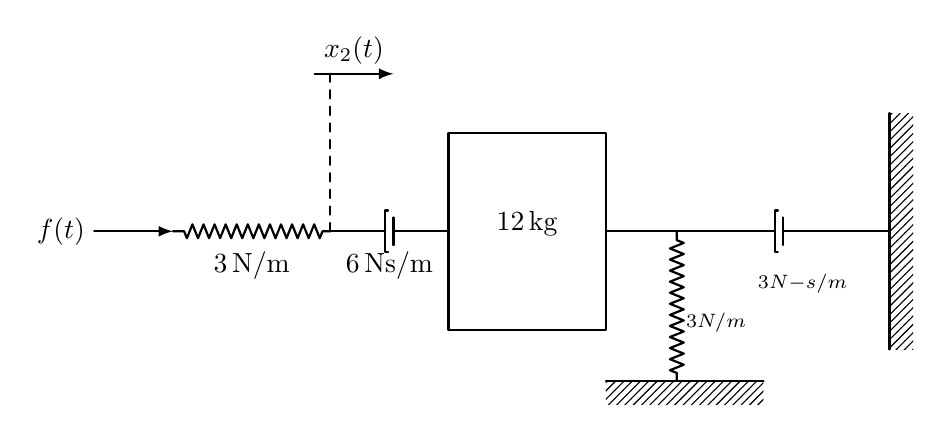
\begin{tikzpicture}[every node/.style={draw,outer sep=0pt,thick}]
		\tikzstyle{spring}=[thick,decorate,decoration={zigzag,pre length=0.1cm,post length=0.1cm,segment length=4}]
		\tikzstyle{damper}=[thick,decoration={markings,
		  mark connection node=dmp,
		  mark=at position 0.5 with
		  {
			\node (dmp) [thick,inner sep=0pt,transform shape,rotate=90,minimum width=15pt,minimum height=3pt,draw=none] {};
			\draw [thick] ($(dmp.north east)+(2pt,0)$) -- (dmp.south east) -- (dmp.south west) -- ($(dmp.north west)+(2pt,0)$);
			\draw [thick] ($(dmp.north)+(0,-5pt)$) -- ($(dmp.north)+(0,5pt)$);
		  }
		}, decorate]
		\tikzstyle{ground}=[fill,pattern=north east lines,draw=none,minimum width=0.75cm,minimum height=0.3cm]
	
		\begin{scope}[xshift=7cm]
			% Mass block
			\node (M) [minimum width=2cm, minimum height=2.5cm, draw, fill=white] {%
				$\begin{array}{c}
					12 \, \mathrm{kg}\\[5pt]
				\end{array}$
			};
	
			\node (wall) [ground, rotate=90, minimum width=3cm, yshift=-4.75cm] {};
			\draw (wall.north east) -- (wall.north west);

			\node (wall2) [ground, rotate=0, minimum width=2cm,yshift=-2.05cm,xshift=2cm] {};
			\draw (wall2.north east) -- (wall2.north west);

			\draw [thick] (M.east) -- ++(1.cm,0) 
				node [midway,yshift=-4pt, below,draw=none] {$ $};

				
				\draw [xshift=4.6cm,damper]++ (0,0) -- +(-2.8cm,0) node [midway, yshift=-12pt, xshift=1cm, below left, draw=none] {$_{3N-s/m}$};

				\draw [xshift=1.9cm,yshift=-1.9cm,rotate=90,spring]++ (0,0) -- +(1.9cm,0) node [midway, yshift=-6pt, right, draw=none] {$_{3N/m}$};

			\draw [damper] (M.west) -- ++(-1.5cm,0) 
				node [midway,yshift=-4pt, below,draw=none] {$6 \, \mathrm{Ns/m}$};
	
			\draw [-latex,thick] ([xshift=-1.7cm,yshift=2cm] M.west) -- ++(1cm,0)
			node [midway,above,draw=none] {$x_2(t)$};
			\draw [dashed] ([xshift=-1.5cm] M.west) -- +(0cm,2cm);

			\draw [spring] ([xshift=-1.5cm] M.west) -- ++(-2cm,0) 
				node [midway,yshift=-4pt, below,draw=none] {$3 \, \mathrm{N/m}$};
	
			\draw [-latex,thick] ([xshift=-4.5cm] M.west) -- ++(1cm,0) 
				node [midway,left,xshift=-.5cm,draw=none] {$f(t)$};
		\end{scope}
	\end{tikzpicture}
	
\end{center}


	\rule{\textwidth}{1pt}

\noindent\textbf{Given:} As per diagram

\vspace{12pt}
\noindent\textit{\textbf{Solution:}}

\vspace{12pt}

Force Balance on M:\\
\begin{center}
	$M\ddot{x}(t)+(b_1+b_2)\dot{x}(t)+(k_1+k_2)x(t)=f(t)$\\
\end{center}
Laplace Transform:\\
\begin{center}
	$Ms^2X(s)+(b_1+b_2)sX(s)+(k_1+k_2)X(s)=F(s)$\\
\end{center}
Substitute the Given Values:\\
\begin{center}
	$12s^2X(s)+(6+3)sX(s)+(3+3)X(s)=F(s)$\\
\end{center}
Simplify:\\
\begin{center}
	$12s^2X(s)+9sX(s)+6X(s)=F(s)$\\
\end{center}
Transfer function solving for $\dfrac{X(s)}{F(s)}:$\\
\begin{center}
	\begin{tabular}{|c|}
		\hline \\
		$\dfrac{X(s)}{F(s)}=\dfrac{1}{12s^2+9s+6}$	\\ [12pt]
	\hline
	\end{tabular}	
\end{center}

\clearpage

\rule{\textwidth}{1pt}
\textbf{Problem 37}\\
Find the transfer function, $\dfrac{X_1(s)}{F(s)}$ \\

\begin{center}
	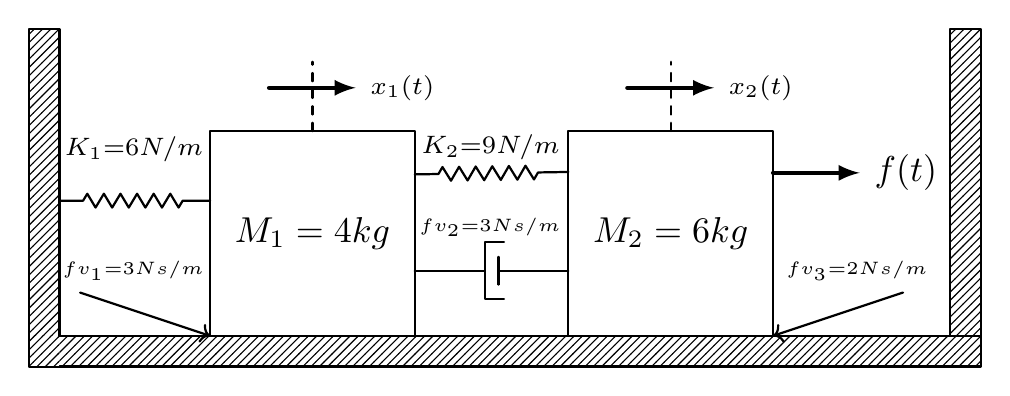
\begin{tikzpicture}[scale=1.1, every node/.style={scale=1.3}]
		\tikzstyle{spring}=[thick,decorate,decoration={zigzag,pre length=0.3cm,post length=0.3cm,segment length=6}]
		\tikzstyle{damper}=[thick,decoration={markings,  
			mark connection node=dmp,
			mark=at position 0.5 with 
			{
				\node (dmp) [thick,inner sep=0pt,transform shape,rotate=-90,minimum width=15pt,minimum height=3pt,draw=none] {};
				\draw [thick] ($(dmp.north east)+(2pt,0)$) -- (dmp.south east) -- (dmp.south west) -- ($(dmp.north west)+(2pt,0)$);
				\draw [thick] ($(dmp.north)+(0,-5pt)$) -- ($(dmp.north)+(0,5pt)$);
			}
		}, decorate]
		\tikzstyle{ground}=[fill,pattern=north east lines,draw=none,minimum width=0.75cm,minimum height=0.3cm,inner sep=0pt,outer sep=0pt]
	
		\node [draw, outer sep=0pt, thick] (M) [minimum width=2cm, minimum height=2cm] {$M_1=4 kg$};
		\node [draw, outer sep=0pt, thick] (M2) [minimum width=2cm, minimum height=2cm, xshift = 3.5cm] {$M_2=6 kg$};
	
		\node (ground) [ground,anchor=north,yshift=-0.0cm,minimum width=9cm,xshift=2.03cm] at (M.south) {};
		\draw (ground.north west) -- (ground.north east) -- (ground.south east) -- (ground.south west);
	
		\node (fill) [ground,xshift=-0.15cm,minimum height = 0.3cm, minimum width = 0.3cm] at (ground.west) {};
		\draw (fill.north west) -- (fill.south west) -- (fill.south east);
	
		\draw [spring] (M.30) -- (M2.-211) node (k) [midway,above] {$_{K_2=9N/m}$};
		\draw [damper] (M.-20) -- (M2.-160) node (k) [midway,above,yshift=0.2cm] {$_{_{f{v_2}=3Ns/m}}$};
	
		\node (wall) [ground, rotate=-90, minimum width=3cm,anchor=south east] at (fill.north west) {};
		\draw (wall.north east) -- (wall.north west) -- (wall.south west) -- (wall.south east);
	
		\node (wall2) [ground, rotate=-90, minimum width=3cm,anchor=north east,yshift=9cm] at (fill.north east) {};
		\draw (wall2.north east) -- (wall2.north west) -- (wall2.south west) -- (wall2.south east);
	
		\draw [->, thick] 
    ($(M.south west) + (-1.5cm, 0.5cm)$) -- ($(M.south west) + (0cm, 0cm)$)
    node [midway,above,yshift=0.2cm,xshift=-0.1cm] {$_{_{f{v_1}=3Ns/m}}$};

	\draw [->, thick] 
    ($(M2.south east) + (1.5cm, 0.5cm)$) -- ($(M2.south east) + (0cm, 0cm)$)
	node [midway,above,yshift=0.2cm,xshift=0.2cm] {$_{_{f{v_3}=2Ns/m}}$};

	
		\draw [spring] (wall.40) -- ($(M.north west)!(wall.40)!(M.south west)$) node [midway,yshift=0.5cm] {$_{K_1=6N/m}$};
		
		\draw [-latex,ultra thick] (M.north) ++(-0.5cm, 0.5cm) -- +(1cm,0cm) node [right,draw=none] (y1) {$_{x_1(t)}$};
		\draw [dashed] (M.north) -- +(0cm,0.8cm);
	
		\draw [-latex,ultra thick] (M2.north) ++(-0.5cm, 0.5cm) -- +(1cm,0cm) node [right,draw=none] (y1) {$_{x_2(t)}$};
		\draw [dashed](M2.north) -- +(0cm,0.8cm);;

		\draw [-latex,ultra thick] (M2.east) ++(0cm, 0.7cm) -- +(1cm,0cm) node [right,draw=none] (y1) {$f(t)$};
	
		
	\end{tikzpicture}
	\end{center}
	
	\rule{\textwidth}{1pt}

\noindent\textbf{Given:} As per diagram

\vspace{12pt}
\noindent\textit{\textbf{Solution:}}

\vspace{12pt}

Equation of Motion:\\[12pt]
For $M_1$:\\
\begin{center}
	$M_1\ddot{x}_1(t)=F_{v1}\dot{x}_1(t)-k_1x_1(t)+F_{v2}[\dot{x}_2(t)-\dot{x}_1(t)]+k_2[x_2(t)-x_1(t)]$\\[12pt]
\end{center}
Substitute :\\
\begin{center}
	$4\ddot{x}_1(t)=-3\dot{x}_1(t)-6x_1(t)+3[\dot{x}_2(t)-\dot{x}_1(t)]+9[x_2(t)-x_1(t)]$\\[12pt]
\end{center}
Simplify:\\
\begin{center}
	$4\ddot{x}_1(t)=-6\dot{x}_1(t)-15x_1(t)+3\dot{x}_2(t)+9x_2(t)$\\[12pt]
\end{center}
For $M_2$:\\
\begin{center}
	$M_2\ddot{x}_2(t)=-F_{v2}[\dot{x}_2(t)-\dot{x}_1(t)]-k_2[x_2(t)-x_1(t)]-f_{v3}\dot{x}_2(t)+F(t)$\\[12pt]
\end{center}
Substitute :\\
\begin{center}
	$6\ddot{x}_2(t)=-3[\dot{x}_2(t)-\dot{x}_1(t)]-9[x_2(t)-x_1(t)]-2\dot{x}_2(t)+F(t)$\\[12pt]
\end{center}
Simplify:\\
\begin{center}
	$6\ddot{x}_2(t)=-5\dot{x}_2(t)+3\dot{x}_1(t)-9x_2(t)+9x_1(t)+F(t)$\\[12pt]
\end{center}
Apply the Laplace Transform for $M_1$ and $M_2$\\[12pt]
For $M_1$:\\[12pt]
\begin{center}
	$(4s^2+6s+15)X_1(s)=(3s+9)X_2(s)$\\
\end{center}
For $M_2$\\
\begin{center}
	$(6s^2+5s+9)X_2(s)=(3s+9)X_1(s)+F(s)$\\[12pt]
\end{center}
Solve for $G(s)=\dfrac{X_1(s)}{F(s)}$:\\
\begin{center}
	$X_2(s)=\dfrac{(3s+9)X_1(s)+F(s)}{6s^2+5s+9}$\\
\end{center}
Substitute $X_2(s)$ to $X_1(s)$\\
\begin{center}
	$(4s^2+6s+15)X_1(s)=\dfrac{(3s+9)^2X_1(s)+(3s+9)F(s)}{6s^2+5s+9}$\\[12pt]
	$(4s^2+6s+15)(6s^2+5s+9)X_1(s)=(9s^2+54s+81)X_1(s)+(3s+9)F(s)$\\
\end{center}
Simplify:\\
\begin{center}
	$(24s^4+44s^3+111s^2+135s+135)X_1(s)=(9s^2+54s+81)X_1(s)+(3s+9)F(s)$\\[12pt]
	$(24s^4+44s^3+102s^2+81s+54)X_1(s)=(3s+9)F(s)$\\
\end{center}
Thus $G(s)=\dfrac{X_1(s)}{F(s)}$\\
\begin{center}
	\begin{tabular}{|c|}
		\hline \\
		$G(s)=\dfrac{3s+9}{24s^4+44s^3+102s^2+81s+54}$	\\ [12pt]
	\hline
	\end{tabular}	
\end{center}

\clearpage

\rule{\textwidth}{1pt}
\textbf{Problem 38}\\
Find the transfer function, $\dfrac{X(s)}{F(s)}$ \\

\begin{center}
	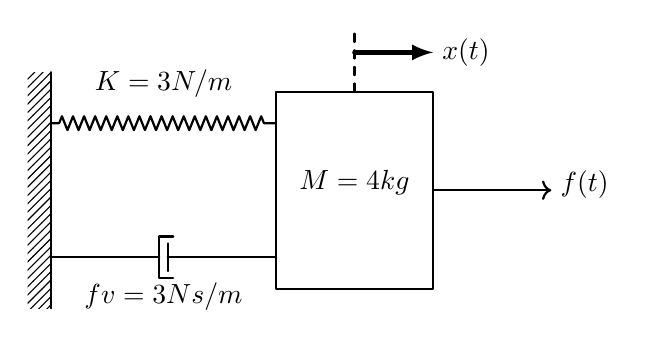
\begin{tikzpicture}[every node/.style={draw,outer sep=0pt,thick}]
		\tikzstyle{spring}=[thick,decorate,decoration={zigzag,pre length=0.1cm,post length=0.1cm,segment length=4}]
		\tikzstyle{damper}=[thick,decoration={markings,
		  mark connection node=dmp,
		  mark=at position 0.5 with
		  {
			\node (dmp) [thick,inner sep=0pt,transform shape,rotate=-90,minimum width=15pt,minimum height=3pt,draw=none] {};
			\draw [thick] ($(dmp.north east)+(2pt,0)$) -- (dmp.south east) -- (dmp.south west) -- ($(dmp.north west)+(2pt,0)$);
			\draw [thick] ($(dmp.north)+(0,-5pt)$) -- ($(dmp.north)+(0,5pt)$);
		  }
		}, decorate]
		\tikzstyle{ground}=[fill,pattern=north east lines,draw=none,minimum width=0.75cm,minimum height=0.3cm]
	
		\begin{scope}[xshift=7cm]
			\node (M) [minimum width=2cm, minimum height=2.5cm, draw, fill=white] {$			\begin{array}{c}
				M = 4 kg\\[5pt]
				
			\end{array}$};

			\draw [-latex,ultra thick] (M.north) ++(0cm, 0.5cm) -- +(1cm,0cm) node [right,draw=none] (y1) {$x(t)$};
			\draw [dashed] (M.north) -- +(0cm,0.8cm);
	

		\node (wall) [ground, rotate=-90, minimum width=3cm,yshift=-4cm] {};
		\draw (wall.north east) -- (wall.north west);
	
	
		\draw [spring] (wall.170) -- ($(M.north west)!(wall.170)!(M.south west)$) node [midway,yshift=6pt, above,draw=none] {$K=3 N/m$};
		\draw [damper] (wall.10) -- ($(M.north west)!(wall.10)!(M.south west)$) node [midway,yshift=-6pt, below,draw=none] {$fv=3 Ns/m$};
	
		\draw [->] (M.east) ++ (0,0) -- +(1.5cm,0) node[right,yshift=2pt, draw=none] {$f(t)$};
		\end{scope}
	\end{tikzpicture}
	\end{center}


	
	\rule{\textwidth}{1pt}

\noindent\textbf{Given:} As per diagram

\vspace{12pt}
\noindent\textit{\textbf{Solution:}}

\vspace{12pt}

Equation of Motion:\\
\begin{center}
	$M\dfrac{d^2x(t)}{dt^2}+fv\dfrac{dx(t)}{dt}+Kx(t)=f(t)$\\[12pt]
\end{center}
Substitute the Given:\\
\begin{center}
	$4\dfrac{d^2x(t)}{dt^2}+3\dfrac{dx(t)}{dt}+3x(t)=f(t)$\\[12pt]
\end{center}
Laplace Transform:\\[12pt]
(Consider that the Initial Conditionis 0)\\
\begin{center}
	$4s^2X(s)+3sX(s)+3X(s)=F(s)$\\[12pt]
\end{center}
Transfer function $\dfrac{X(s)}{F(s)}$\\
\begin{center}
	\begin{tabular}{|c|}
		\hline \\
		$\dfrac{X(s)}{F(s)}=\dfrac{1}{4s^2+3s+3}$	\\ [12pt]
	\hline
	\end{tabular}	
\end{center}

\clearpage
\rule{\textwidth}{1pt}
\textbf{Problem 39}\\
Find the transfer function $\dfrac{X_2(s)}{F(s)}$\\

\begin{center}
	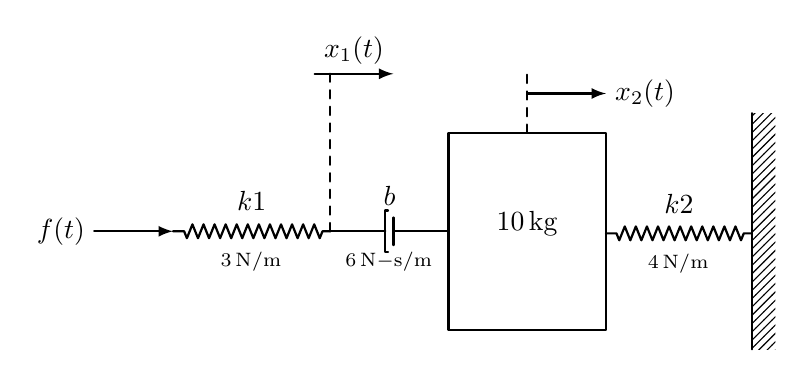
\begin{tikzpicture}[every node/.style={draw,outer sep=0pt,thick}]
		\tikzstyle{spring}=[thick,decorate,decoration={zigzag,pre length=0.1cm,post length=0.1cm,segment length=4}]
		\tikzstyle{damper}=[thick,decoration={markings,
		  mark connection node=dmp,
		  mark=at position 0.5 with
		  {
			\node (dmp) [thick,inner sep=0pt,transform shape,rotate=90,minimum width=15pt,minimum height=3pt,draw=none] {};
			\draw [thick] ($(dmp.north east)+(2pt,0)$) -- (dmp.south east) -- (dmp.south west) -- ($(dmp.north west)+(2pt,0)$);
			\draw [thick] ($(dmp.north)+(0,-5pt)$) -- ($(dmp.north)+(0,5pt)$);
		  }
		}, decorate]
		\tikzstyle{ground}=[fill,pattern=north east lines,draw=none,minimum width=0.75cm,minimum height=0.3cm]
	
		\begin{scope}[xshift=7cm]
			% Mass block
			\node (M) [minimum width=2cm, minimum height=2.5cm, draw, fill=white] {%
				$\begin{array}{c}
					10 \, \mathrm{kg}\\[5pt]
				\end{array}$
			};
	
			\node (wall) [ground, rotate=90, minimum width=3cm, yshift=-3cm] {};
			\draw (wall.north east) -- (wall.north west);
			\draw [spring] (wall.100) -- ($(M.north east)!(wall.100)!(M.south east)$) 
				node [midway,yshift=-4pt, below,draw=none] {$_{4 \, \mathrm{N/m}}$}
				node [midway,yshift=4pt, above,draw=none] {$k2$};
	
			\draw [damper] (M.west) -- ++(-1.5cm,0) 
				node [midway,yshift=-4pt, below,draw=none] {$_{6 \, \mathrm{N-s/m}}$}
				node [midway,yshift=6pt, above,draw=none] {$b$};
	
			\draw [-latex,thick] ([xshift=-1.7cm,yshift=2cm] M.west) -- ++(1cm,0)
			node [midway,above,draw=none] {$x_1(t)$};
			\draw [dashed] ([xshift=-1.5cm] M.west) -- +(0cm,2cm);

			\draw [-latex,thick] (M.north) ++(0cm, 0.5cm) -- +(1cm,0cm) node [right,draw=none] (y1) {$x_2(t)$};
			\draw [dashed] (M.north) -- +(0cm,0.8cm);

			\draw [spring] ([xshift=-1.5cm] M.west) -- ++(-2cm,0) 
				node [midway,yshift=-4pt, below,draw=none] {$_{3 \, \mathrm{N/m}}$}
				node [midway,yshift=4pt, above,draw=none] {$k1$};
	
			\draw [-latex,thick] ([xshift=-4.5cm] M.west) -- ++(1cm,0) 
				node [midway,left,xshift=-.5cm,draw=none] {$f(t)$};
		\end{scope}
	\end{tikzpicture}
\end{center}

\rule{\textwidth}{1pt}

\noindent\textbf{Given:} As per diagram

\vspace{12pt}
\noindent\textit{\textbf{Solution:}}

\vspace{12pt}

Equation for $X_1(t)$:\\
\begin{center}
	$F(t)-k_1x_1(t)-b[\dot{x}_1(t)-\dot{x}_2(t)]=0$\\[12pt]
\end{center}
Apply the Laplace Transform:\\
\begin{center}
	$F(s)-k_1X_1(s)-b[sX_1(s)-sX_2(s)]=0$\\
\end{center}
Simplify:\\
\begin{center}
	$F(s)=(k_1+bs)X_1(s)-bsX_2(s)$\\
\end{center}
Equation for $X_2(t)$:\\
\begin{center}
	$b[\dot{x}_1(t)-\dot{x}_2(t)]+k_2x_2(t)=M\ddot{x}_2(t)$\\
\end{center}
Apply Laplace Transform:\\
\begin{center}
	$b[sX_1(s)-sX_2(s)]+k_2X_2(s)=Ms^2X_2(s)$\\
\end{center}
Simplify:\\
\begin{center}
	$bsX_1(s)-(bs+k_2)X_2(s)=Ms^2X_2(s)$\\
\end{center}
Solving for $\dfrac{X_2(s)}{F(s)}:$\\[12pt]
$X_1(s):$\\
\begin{center}
	$X_1(s)=\dfrac{F(s)+bsX_2(s)}{k_1+bs}$
\end{center}
Substitute $X_1(s)$ to $2^{nd}$ Equation:\\
\begin{center}
	$b\left(s\dfrac{F(s)+bsX_2(s)}{k_1+bs}\right)-(bs+k_2)X_2(s)=Ms^2X_2(s)$
\end{center}
Simplify:\\
\begin{center}
	$\dfrac{bsF(s)}{k_1+bs}+\dfrac{b^2s^2X_2(s)}{k_1+bs}-(bs+k_2)X_2(s)=Ms^2X_2(s)$
\end{center}
Multiply Both Sides By $(k_1+bs)$:\\
\begin{center}
	$bsF(s)+b^2s^2X_2(s)-(bs+k_2)(k_1+bs)X_2(s)=Ms^2(k_1+bs)X_2(s)$\\
\end{center}
Collecting Terms:\\
\begin{center}
	$bsF(s)=[Ms^2(k_1+bs)+(bs+k_2)(k_1+bs)-b^2s^2]X_2(s)$\\
\end{center}
Hence:\\
\begin{center}
	$\dfrac{X_2(s)}{F(s)}=\dfrac{bs}{Ms^2(k_1+bs)+(bs+k_2)(k_1+bs)-b^2s^2}$\\
\end{center}

Substitute the Given Values:\\
\begin{center}
	$\dfrac{X_2(s)}{F(s)}=\dfrac{6s}{10s^2(3+6s)+(6s+4)(3+6s)-36s^2}$\\[12pt]
	Or\\[12pt]
	\begin{tabular}{|c|}
		\hline \\
		$\dfrac{X_2(s)}{F(s)}=\dfrac{6s}{60s^3+30s^2+(36s^2+42s+12)-36s^2}$\\[12pt]
		\hline
	\end{tabular}	
\end{center}

\clearpage

\rule{\textwidth}{1pt}
\textbf{Problem 40}\\
Find the transfer function, $G(s)=\dfrac{X_1(s)}{F(s)}$ for the translational mechanical system shown in Figure\\

\begin{center}
	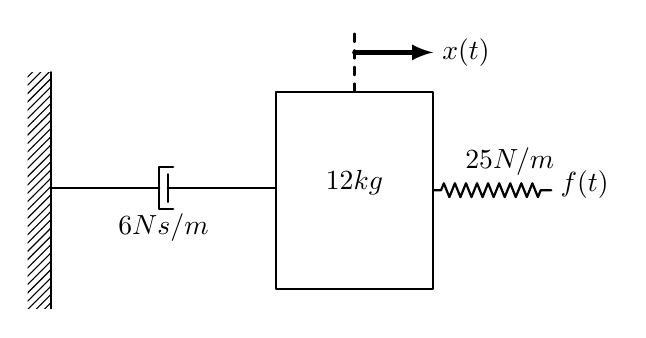
\begin{tikzpicture}[every node/.style={draw,outer sep=0pt,thick}]
		\tikzstyle{spring}=[thick,decorate,decoration={zigzag,pre length=0.1cm,post length=0.1cm,segment length=4}]
		\tikzstyle{damper}=[thick,decoration={markings,
		  mark connection node=dmp,
		  mark=at position 0.5 with
		  {
			\node (dmp) [thick,inner sep=0pt,transform shape,rotate=-90,minimum width=15pt,minimum height=3pt,draw=none] {};
			\draw [thick] ($(dmp.north east)+(2pt,0)$) -- (dmp.south east) -- (dmp.south west) -- ($(dmp.north west)+(2pt,0)$);
			\draw [thick] ($(dmp.north)+(0,-5pt)$) -- ($(dmp.north)+(0,5pt)$);
		  }
		}, decorate]
		\tikzstyle{ground}=[fill,pattern=north east lines,draw=none,minimum width=0.75cm,minimum height=0.3cm]
	
		\begin{scope}[xshift=7cm]
			\node (M) [minimum width=2cm, minimum height=2.5cm, draw, fill=white] {$			\begin{array}{c}
				12 kg\\[5pt]
			\end{array}$};

			\draw [-latex,ultra thick] (M.north) ++(0cm, 0.5cm) -- +(1cm,0cm) node [right,draw=none] (y1) {$x(t)$};
			\draw [dashed] (M.north) -- +(0cm,0.8cm);
	
			\node (wall) [ground, rotate=-90, minimum width=3cm,yshift=-4cm] {};
			\draw (wall.north east) -- (wall.north west);
	
			\draw [damper] (wall.100) -- ($(M.north west)!(wall.100)!(M.south west)$) node [midway,yshift=-6pt, below,draw=none] {$6 Ns/m$};
	
			\draw [spring] (M.east) ++ (0,0) -- +(1.5cm,0)node[xshift=-15pt,yshift=2pt,above, draw=none] {$25 N/m$} node[right,yshift=2pt, draw=none] {$f(t)$};
		\end{scope}
	\end{tikzpicture}
\end{center}

\rule{\textwidth}{1pt}

\noindent\textbf{Given:} As per diagram

\vspace{12pt}
\noindent\textit{\textbf{Solution:}}

\vspace{12pt}

Equation of Motion:\\
\begin{center}
	$M\ddot{x}(t)=F(t)-F_{s}-F_{d}$\\[12pt]
\end{center}
Substitute the Given Values:\\
\begin{center}
	$12\ddot{x}(t)=F(t)-25x(t)-6\dot{x}(t)$\\
\end{center}
Apply the Laplace Transform (zero initial conditions):\\
\begin{center}
	$12s^2X(s)=F(s)-25X(s)-6sX(s)$\\[12pt]
\end{center}
Rearrange:\\
\begin{center}
	$X(s)(12s^2+6s+25)=F(s)$\\
\end{center}
Final Transfer Function:\\
\begin{center}
	\begin{tabular}{|c|}
		\hline \\
		$G(s)=\dfrac{1}{12s^2+6s+25}$\\[12pt]
		\hline
	\end{tabular}	
\end{center}

\clearpage

\rule{\textwidth}{1pt}
\textbf{Problem 41}\\
Find the transfer function, $G(s)=\dfrac{X_1(s)}{F(s)}$ for the translational mechanical system shown in Figure\\

\begin{center}
	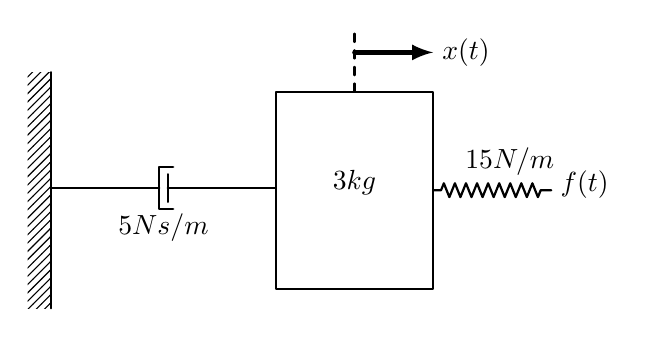
\begin{tikzpicture}[every node/.style={draw,outer sep=0pt,thick}]
		\tikzstyle{spring}=[thick,decorate,decoration={zigzag,pre length=0.1cm,post length=0.1cm,segment length=4}]
		\tikzstyle{damper}=[thick,decoration={markings,
		  mark connection node=dmp,
		  mark=at position 0.5 with
		  {
			\node (dmp) [thick,inner sep=0pt,transform shape,rotate=-90,minimum width=15pt,minimum height=3pt,draw=none] {};
			\draw [thick] ($(dmp.north east)+(2pt,0)$) -- (dmp.south east) -- (dmp.south west) -- ($(dmp.north west)+(2pt,0)$);
			\draw [thick] ($(dmp.north)+(0,-5pt)$) -- ($(dmp.north)+(0,5pt)$);
		  }
		}, decorate]
		\tikzstyle{ground}=[fill,pattern=north east lines,draw=none,minimum width=0.75cm,minimum height=0.3cm]
	
		\begin{scope}[xshift=7cm]
			\node (M) [minimum width=2cm, minimum height=2.5cm, draw, fill=white] {$			\begin{array}{c}
				3 kg\\[5pt]
			\end{array}$};

			\draw [-latex,ultra thick] (M.north) ++(0cm, 0.5cm) -- +(1cm,0cm) node [right,draw=none] (y1) {$x(t)$};
			\draw [dashed] (M.north) -- +(0cm,0.8cm);
	
			\node (wall) [ground, rotate=-90, minimum width=3cm,yshift=-4cm] {};
			\draw (wall.north east) -- (wall.north west);
	
			\draw [damper] (wall.100) -- ($(M.north west)!(wall.100)!(M.south west)$) node [midway,yshift=-6pt, below,draw=none] {$5 Ns/m$};
	
			\draw [spring] (M.east) ++ (0,0) -- +(1.5cm,0)node[xshift=-15pt,yshift=2pt,above, draw=none] {$15 N/m$} node[right,yshift=2pt, draw=none] {$f(t)$};
		\end{scope}
	\end{tikzpicture}
\end{center}

\rule{\textwidth}{1pt}

\noindent\textbf{Given:} As per diagram

\vspace{12pt}
\noindent\textit{\textbf{Solution:}}

\vspace{12pt}

Equation of Motion:\\
\begin{center}
	$M\ddot{x}(t)=F(t)-F_{s}-F_{d}$\\[12pt]
\end{center}
Substitute the Given Values:\\
\begin{center}
	$3\ddot{x}(t)=F(t)-15x(t)-5\dot{x}(t)$\\
\end{center}
Apply the Laplace Transform (zero initial conditions):\\
\begin{center}
	$3s^2X(s)=F(s)-15X(s)-5sX(s)$\\[12pt]
\end{center}
Rearrange:\\
\begin{center}
	$X(s)(3s^2+5s+15)=F(s)$\\
\end{center}
Final Transfer Function:\\
\begin{center}
	\begin{tabular}{|c|}
		\hline \\
		$G(s)=\dfrac{1}{3s^2+5s+15}$\\[12pt]
		\hline
	\end{tabular}	
\end{center}

\clearpage
\rule{\textwidth}{1pt}
\textbf{Problem 42}\\
For the translational mechanical system shown below, find the transfer function $G(s)=\dfrac{X_2(s)}{F(s)}$\\

\begin{center}
	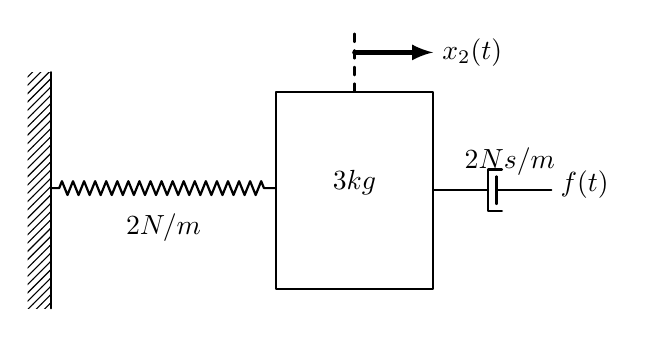
\begin{tikzpicture}[every node/.style={draw,outer sep=0pt,thick}]
		\tikzstyle{spring}=[thick,decorate,decoration={zigzag,pre length=0.1cm,post length=0.1cm,segment length=4}]
		\tikzstyle{damper}=[thick,decoration={markings,
		  mark connection node=dmp,
		  mark=at position 0.5 with
		  {
			\node (dmp) [thick,inner sep=0pt,transform shape,rotate=-90,minimum width=15pt,minimum height=3pt,draw=none] {};
			\draw [thick] ($(dmp.north east)+(2pt,0)$) -- (dmp.south east) -- (dmp.south west) -- ($(dmp.north west)+(2pt,0)$);
			\draw [thick] ($(dmp.north)+(0,-5pt)$) -- ($(dmp.north)+(0,5pt)$);
		  }
		}, decorate]
		\tikzstyle{ground}=[fill,pattern=north east lines,draw=none,minimum width=0.75cm,minimum height=0.3cm]
	
		\begin{scope}[xshift=7cm]
			\node (M) [minimum width=2cm, minimum height=2.5cm, draw, fill=white] {$			\begin{array}{c}
				3 kg\\[5pt]
			\end{array}$};

			\draw [-latex,ultra thick] (M.north) ++(0cm, 0.5cm) -- +(1cm,0cm) node [right,draw=none] (y1) {$x_2(t)$};
			\draw [dashed] (M.north) -- +(0cm,0.8cm);
	
			\node (wall) [ground, rotate=-90, minimum width=3cm,yshift=-4cm] {};
			\draw (wall.north east) -- (wall.north west);
	
			\draw [spring] (wall.100) -- ($(M.north west)!(wall.100)!(M.south west)$) node [midway,yshift=-6pt, below,draw=none] {$2 N/m$};
	
			\draw [damper] (M.east) ++ (0,0) -- +(1.5cm,0)node[xshift=-15pt,yshift=2pt,above, draw=none] {$2 Ns/m$} node[right,yshift=2pt, draw=none] {$f(t)$};
		\end{scope}
	\end{tikzpicture}
\end{center}

\rule{\textwidth}{1pt}

\noindent\textbf{Given:} As per diagram

\vspace{12pt}
\noindent\textit{\textbf{Solution:}}

\vspace{12pt}

Equation of Motion:\\
\begin{center}
	$M\ddot{x}_2(t)=F(t)-F_s-F_d$\\[12pt]
\end{center}
Apply Laplace Transform:\\
\begin{center}
	$3s^2X_2(s)=F(s)-2X_2(s)-2sX_2(s)$\\
\end{center}
Simplify:\\
\begin{center}
	$3s^2X_2(s)+2sX_2(s)+2X_2(s)=F(s)$\\[12pt]
	$X_2(s)(3s^2+2s+2)=F(s)$\\[12pt]
\end{center}
Thus $G(s)=\dfrac{X_2(s)}{F(s)}$\\
\begin{center}
	\begin{tabular}{|c|}
		\hline \\
		$G(s)=\dfrac{1}{3s^2+2s+2}$\\[12pt]
		\hline
	\end{tabular}	
\end{center}

\clearpage

\rule{\textwidth}{1pt}
\textbf{Problem 43}\\
Find the transfer function $G(s)=\dfrac{X_2(s)}{F(s)}$\\

\begin{center}
	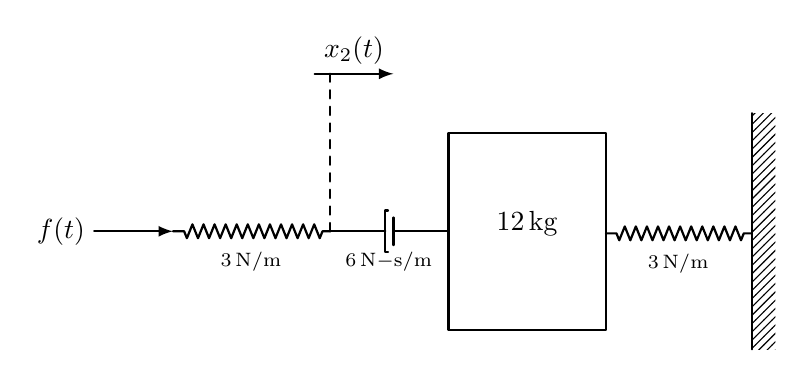
\begin{tikzpicture}[every node/.style={draw,outer sep=0pt,thick}]
		\tikzstyle{spring}=[thick,decorate,decoration={zigzag,pre length=0.1cm,post length=0.1cm,segment length=4}]
		\tikzstyle{damper}=[thick,decoration={markings,
		  mark connection node=dmp,
		  mark=at position 0.5 with
		  {
			\node (dmp) [thick,inner sep=0pt,transform shape,rotate=90,minimum width=15pt,minimum height=3pt,draw=none] {};
			\draw [thick] ($(dmp.north east)+(2pt,0)$) -- (dmp.south east) -- (dmp.south west) -- ($(dmp.north west)+(2pt,0)$);
			\draw [thick] ($(dmp.north)+(0,-5pt)$) -- ($(dmp.north)+(0,5pt)$);
		  }
		}, decorate]
		\tikzstyle{ground}=[fill,pattern=north east lines,draw=none,minimum width=0.75cm,minimum height=0.3cm]
	
		\begin{scope}[xshift=7cm]
			% Mass block
			\node (M) [minimum width=2cm, minimum height=2.5cm, draw, fill=white] {%
				$\begin{array}{c}
					12 \, \mathrm{kg}\\[5pt]
				\end{array}$
			};
	
			\node (wall) [ground, rotate=90, minimum width=3cm, yshift=-3cm] {};
			\draw (wall.north east) -- (wall.north west);
			\draw [spring] (wall.100) -- ($(M.north east)!(wall.100)!(M.south east)$) 
				node [midway,yshift=-4pt, below,draw=none] {$_{3 \, \mathrm{N/m}}$};
	
			\draw [damper] (M.west) -- ++(-1.5cm,0) 
				node [midway,yshift=-4pt, below,draw=none] {$_{6 \, \mathrm{N-s/m}}$};
	
			\draw [-latex,thick] ([xshift=-1.7cm,yshift=2cm] M.west) -- ++(1cm,0)
			node [midway,above,draw=none] {$x_2(t)$};
			\draw [dashed] ([xshift=-1.5cm] M.west) -- +(0cm,2cm);

			\draw [spring] ([xshift=-1.5cm] M.west) -- ++(-2cm,0) 
				node [midway,yshift=-4pt, below,draw=none] {$_{3 \, \mathrm{N/m}}$};
	
			\draw [-latex,thick] ([xshift=-4.5cm] M.west) -- ++(1cm,0) 
				node [midway,left,xshift=-.5cm,draw=none] {$f(t)$};
		\end{scope}
	\end{tikzpicture}
\end{center}

\rule{\textwidth}{1pt}

\noindent\textbf{Given:} As per diagram

\vspace{12pt}
\noindent\textit{\textbf{Solution:}}

\vspace{12pt}

For Mass M:\\
\begin{center}
	$M\ddot{x}_2(t)=F(t)-F_{s1}-F_d-F_{s2}$\\[12pt]
	$12\ddot{x}_2(t)=F(t)-3[x_2(t)-x_1(t)]-6\dot{x}_2(t)-3x_2(t)$\\
\end{center}
Simplify:\\
\begin{center}
	$12\ddot{x}_2(t)+6\dot{x}_2(t)+6x_2(t)-3x_1(t)=F(t)$\\
\end{center}
Taking Laplace Transform:\\
\begin{center}
	$12s^2X_2(s)+6sX_2(s)+6X_2(s)-3X_1(s)=F(s)$\\
\end{center}
Solve for $X_2(s)$:\\
\begin{center}
	$X_2(s)(12s^2+6s+6)-3X_1(s)=F(s)$
\end{center}
Relate $X_1(s)$ to $X_2(s)$:\\
\begin{center}
	$3x_1(t)+6\dot{x}_1(t)=F(t)$\\
\end{center}
Laplace Transform:\\
\begin{center}
	$3X_1(s)+6sX_1(s)=F(s)$\\[12pt]
	$X_1(s)(3+6s)=F(s)$\\[12pt]
	$X_1(s)=\dfrac{F(s)}{3+6s}$\\
\end{center}
Substitute $X_1(s)$ Back:\\
\begin{center}
	$X_2(s)(12s^2+6s+6)-3\left(\dfrac{F(s)}{3+6s}\right)=F(s)$\\
\end{center}
Solve for Transfer Function:\\
\begin{center}
	$X_2(s)=\dfrac{F(s)+\left(\frac{3F(s)}{3+6s}\right)}{12s^2+6s+6}$\\[12pt]
\end{center}
Thus $G(s)=\dfrac{X_2(s)}{F(s)}$\\
\begin{center}
	\begin{tabular}{|c|}
		\hline \\
		$G(s)=\dfrac{6s+4}{(3+6s)(12s^2+6s+6)}$\\[12pt]
		\hline
	\end{tabular}	
\end{center}

\clearpage
\rule{\textwidth}{1pt}
\textbf{Problem 44}\\
Determine the transfer function $\dfrac{X(s)}{F(s)}$ of the system below\\
\begin{center}
	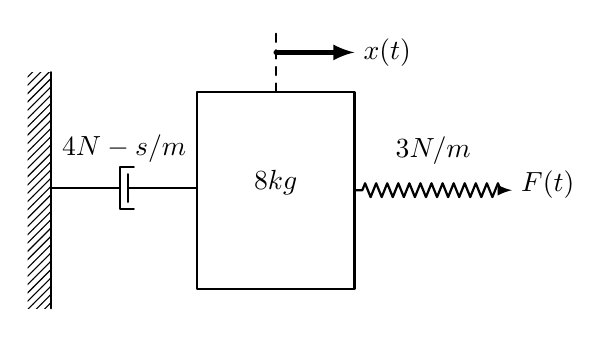
\begin{tikzpicture}[every node/.style={draw,outer sep=0pt,thick}]
		\tikzstyle{spring}=[thick,decorate,decoration={zigzag,pre length=0.1cm,post length=0.1cm,segment length=4}]
		\tikzstyle{damper}=[thick,decoration={markings,
		  mark connection node=dmp,
		  mark=at position 0.5 with
		  {
			\node (dmp) [thick,inner sep=0pt,transform shape,rotate=-90,minimum width=15pt,minimum height=3pt,draw=none] {};
			\draw [thick] ($(dmp.north east)+(2pt,0)$) -- (dmp.south east) -- (dmp.south west) -- ($(dmp.north west)+(2pt,0)$);
			\draw [thick] ($(dmp.north)+(0,-5pt)$) -- ($(dmp.north)+(0,5pt)$);
		  }
		}, decorate]
		\tikzstyle{ground}=[fill,pattern=north east lines,draw=none,minimum width=0.75cm,minimum height=0.3cm]
	
		\begin{scope}[xshift=7cm]
			\node (M) [minimum width=2cm, minimum height=2.5cm, draw, fill=white] {$			\begin{array}{c}
				8 kg\\[5pt]
			\end{array}$};

			\draw [-latex,ultra thick] (M.north) ++(0cm, 0.5cm) -- +(1cm,0cm) node [right,draw=none] (y1) {$x(t)$};
			\draw [dashed] (M.north) -- +(0cm,0.8cm);
	
			\node (wall) [ground, rotate=-90, minimum width=3cm,yshift=-3cm] {};
			\draw (wall.north east) -- (wall.north west);
	
			\draw [damper] (wall.100) -- ($(M.north west)!(wall.100)!(M.south west)$) node [midway,yshift=6pt, above,draw=none] {$4 N-s/m$};
	
			\draw [-latex,spring] (M.east) ++ (0,0) -- +(2cm,0) node [midway,yshift=6pt, above,draw=none] {$3 N/m$} node[right,yshift=2pt, draw=none] {$F(t)$};
		\end{scope}
	\end{tikzpicture}
\end{center}
\rule{\textwidth}{1pt}

\noindent\textbf{Given:} As per diagram

\vspace{12pt}
\noindent\textit{\textbf{Solution:}}

\vspace{12pt}

Free Body Diagram:	
\begin{center}
	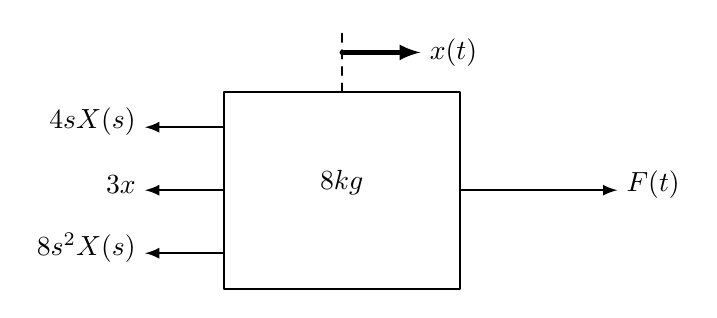
\begin{tikzpicture}[every node/.style={draw,outer sep=0pt,thick}]
	\tikzstyle{spring}=[thick,decorate,decoration={zigzag,pre length=0.1cm,post length=0.1cm,segment length=4}]
	\tikzstyle{damper}=[thick,decoration={markings,
	  mark connection node=dmp,
	  mark=at position 0.5 with
	  {
		\node (dmp) [thick,inner sep=0pt,transform shape,rotate=-90,minimum width=15pt,minimum height=3pt,draw=none] {};
		\draw [thick] ($(dmp.north east)+(2pt,0)$) -- (dmp.south east) -- (dmp.south west) -- ($(dmp.north west)+(2pt,0)$);
		\draw [thick] ($(dmp.north)+(0,-5pt)$) -- ($(dmp.north)+(0,5pt)$);
	  }
	}, decorate]
	\tikzstyle{ground}=[fill,pattern=north east lines,draw=none,minimum width=0.75cm,minimum height=0.3cm]
	
	\begin{scope}[xshift=7cm]
	\node (M) [minimum width=3cm, minimum height=2.5cm, draw, fill=white] {$			\begin{array}{c}
		8 kg\\[5pt]
	\end{array}$};
	\draw [-latex,ultra thick] (M.north) ++(0cm, 0.5cm) -- +(1cm,0cm) node [right,draw=none] (y1) {$x(t)$};
	\draw [dashed] (M.north) -- +(0cm,0.8cm);
	\draw [-latex] (M.east) ++ (0,0) -- +(2cm,0) node[right,yshift=2pt, draw=none] {$F(t)$};
	\draw [-latex] (M.west) ++ (0,0) -- +(-1cm,0) node[left,yshift=2pt, draw=none] {$3x$};
	\draw [-latex] (M.west) ++ (0,0.8) -- +(-1cm,0) node[left,yshift=2pt, draw=none] {$4sX(s)$};
	\draw [-latex] (M.west) ++ (0,-0.8) -- +(-1cm,0) node[left,yshift=2pt, draw=none] {$8s^2X(s)$};
	\end{scope}
	\end{tikzpicture}
\end{center}
Force Balance:\\
\begin{center}
	$F(t)-3x(t)-4\dot{x}(t)-8\ddot{x}(t)=0$\\
\end{center}
Laplace Transform:\\
\begin{center}
	$F(s)-3X(s)-4sX(s)-8s^2X(s)=0$\\[12pt]
	$F(s)=(8s^2+4s+3)X(s)$\\[12pt]
	\boxed{\dfrac{X(s)}{F(s)}=\dfrac{1}{8s^2+4s+3}}
\end{center}

			\clearpage
			\rule{\textwidth}{1pt}
			\textbf{Problem 45}\\
			1. Determine the transfer function $\dfrac{X(s)}{F(s)}$ of the system below\\	

			$K = 4 Nm ; fv = 5 Nm/s ; M = 2 kg$\\
			\begin{center}
			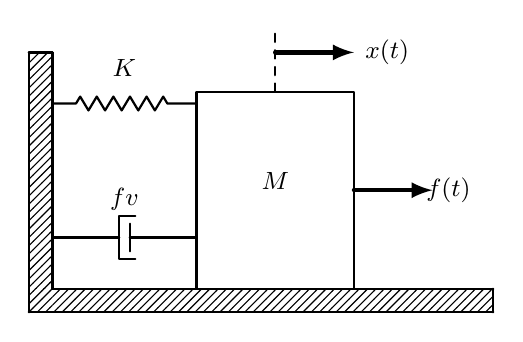
\begin{tikzpicture}
				\tikzstyle{spring}=[thick,decorate,decoration={zigzag,pre length=0.3cm,post length=0.3cm,segment length=6}]
				\tikzstyle{damper}=[thick,decoration={markings,  
				  mark connection node=dmp,
				  mark=at position 0.5 with 
				  {
					\node (dmp) [thick,inner sep=0pt,transform shape,rotate=-90,minimum width=15pt,minimum height=3pt,draw=none] {};
					\draw [thick] ($(dmp.north east)+(2pt,0)$) -- (dmp.south east) -- (dmp.south west) -- ($(dmp.north west)+(2pt,0)$);
					\draw [thick] ($(dmp.north)+(0,-5pt)$) -- ($(dmp.north)+(0,5pt)$);
				  }
				}, decorate]
				\tikzstyle{ground}=[fill,pattern=north east lines,draw=none,minimum width=0.75cm,minimum height=0.3cm,inner sep=0pt,outer sep=0pt]
				
				\node [style={draw,outer sep=0pt,thick}] (M) [minimum width=2cm, minimum height=2.5cm]  {$			\begin{array}{c}
					M\\[5pt]
				\end{array}$};
				\draw [-latex,ultra thick] (M.north) ++(0cm, 0.5cm) -- +(1cm,0cm) node [right,draw=none] (y1) {$x(t)$};
				\draw [dashed] (M.north) -- +(0cm,0.8cm);
				
				\node (ground) [ground,anchor=north,yshift=-0cm,minimum width=5.6cm,xshift=-0.03cm] at (M.south) {};
				\draw (ground.north east) -- (ground.north west);
				\draw (ground.south east) -- (ground.south west);
				\draw (ground.north east) -- (ground.south east);
				
				\node (fill) [ground,xshift=-0.15cm,minimum height = 0.3cm, minimum width = 0.3cm] at (ground.west) {};
				\draw (fill.north west) -- (fill.south west);
				\draw (fill.south west) -- (fill.south east);
				
				
				\node (wall) [ground, rotate=-90, minimum width=3cm,anchor=south east] at (fill.north west) {};
				\draw (wall.north east) -- (wall.north west);
				\draw (wall.north west) -- (wall.south west);
				\draw (wall.south west) -- (wall.south east);
				
				\node (y) at (M.east) [xshift = 1.2cm] {$f(t)$};
				
				\draw [spring] (wall.170) -- ($(M.north west)!(wall.170)!(M.south west)$)node [midway,yshift=6pt, above,draw=none] {$K$};
				\draw [damper] (wall.10) -- ($(M.north west)!(wall.10)!(M.south west)$)node [midway,yshift=6pt, above,draw=none] {$fv$};;
				
				\draw [-latex,ultra thick] (M.east) ++ (0cm,0cm) -- +(1cm,0cm);
				\end{tikzpicture}
			\end{center}
		\rule{\textwidth}{1pt}

\noindent\textbf{Given:} As per diagram

\vspace{12pt}
\noindent\textit{\textbf{Solution:}}

\vspace{12pt}

		FBD of $M$\\	
		\begin{center}
			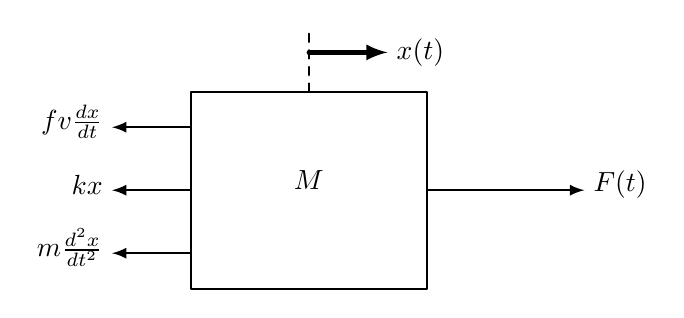
\begin{tikzpicture}[every node/.style={draw,outer sep=0pt,thick}]
			\tikzstyle{spring}=[thick,decorate,decoration={zigzag,pre length=0.1cm,post length=0.1cm,segment length=4}]
			\tikzstyle{damper}=[thick,decoration={markings,
			  mark connection node=dmp,
			  mark=at position 0.5 with
			  {
				\node (dmp) [thick,inner sep=0pt,transform shape,rotate=-90,minimum width=15pt,minimum height=3pt,draw=none] {};
				\draw [thick] ($(dmp.north east)+(2pt,0)$) -- (dmp.south east) -- (dmp.south west) -- ($(dmp.north west)+(2pt,0)$);
				\draw [thick] ($(dmp.north)+(0,-5pt)$) -- ($(dmp.north)+(0,5pt)$);
			  }
			}, decorate]
			\tikzstyle{ground}=[fill,pattern=north east lines,draw=none,minimum width=0.75cm,minimum height=0.3cm]
			
			\begin{scope}[xshift=7cm]
			\node (M) [minimum width=3cm, minimum height=2.5cm, draw, fill=white] {$			\begin{array}{c}
				M\\[5pt]
			\end{array}$};
			\draw [-latex,ultra thick] (M.north) ++(0cm, 0.5cm) -- +(1cm,0cm) node [right,draw=none] (y1) {$x(t)$};
			\draw [dashed] (M.north) -- +(0cm,0.8cm);
			\draw [-latex] (M.east) ++ (0,0) -- +(2cm,0) node[right,yshift=2pt, draw=none] {$F(t)$};
			\draw [-latex] (M.west) ++ (0,0) -- +(-1cm,0) node[left,yshift=2pt, draw=none] {$kx$};
			\draw [-latex] (M.west) ++ (0,0.8) -- +(-1cm,0) node[left,yshift=2pt, draw=none] {$fv\frac{dx}{dt}$};
			\draw [-latex] (M.west) ++ (0,-0.8) -- +(-1cm,0) node[left,yshift=2pt, draw=none] {$m\frac{d^2x}{dt^2}$};
			\end{scope}
			\end{tikzpicture}
			\end{center}
\begin{center}
$\sum F_x=0 \quad \rightarrow \quad \oplus$\\[1ex]

$f(t)-m\frac{d^2x}{dt^2}-fv\frac{dx}{dt}-kx=0$\\[1ex]

$F(s)-2s^2X(s)-5sX(s)-4X(s)=0$\\[1ex]

$F(s)=(2s^2+5s+4)X(s)$\\[1ex]

\boxed{ \dfrac{X(s)}{F(s)} = \dfrac{1}{2s^2 + 5s + 4} }
\end{center}

			\clearpage
			\rule{\textwidth}{1pt}
			\textbf{Problem 46}\\
			1. Determine the transfer function $\dfrac{X(s)}{F(s)}$ of the system below\\	

			$K_1 = 4 Nm ; K_2 = 3 Nm ;  fv = 2 Nm/s ; M = 1 kg$\\
			\begin{center}
			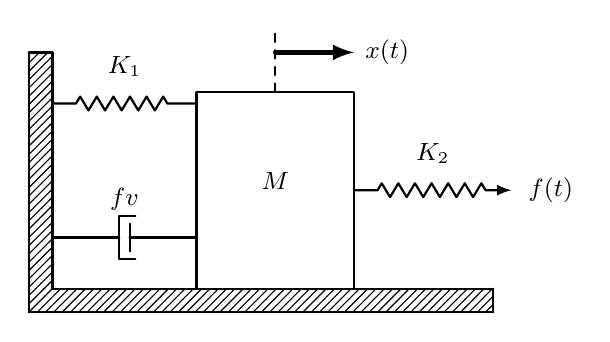
\begin{tikzpicture}
				\tikzstyle{spring}=[thick,decorate,decoration={zigzag,pre length=0.3cm,post length=0.3cm,segment length=6}]
				\tikzstyle{damper}=[thick,decoration={markings,  
				  mark connection node=dmp,
				  mark=at position 0.5 with 
				  {
					\node (dmp) [thick,inner sep=0pt,transform shape,rotate=-90,minimum width=15pt,minimum height=3pt,draw=none] {};
					\draw [thick] ($(dmp.north east)+(2pt,0)$) -- (dmp.south east) -- (dmp.south west) -- ($(dmp.north west)+(2pt,0)$);
					\draw [thick] ($(dmp.north)+(0,-5pt)$) -- ($(dmp.north)+(0,5pt)$);
				  }
				}, decorate]
				\tikzstyle{ground}=[fill,pattern=north east lines,draw=none,minimum width=0.75cm,minimum height=0.3cm,inner sep=0pt,outer sep=0pt]
				
				\node [style={draw,outer sep=0pt,thick}] (M) [minimum width=2cm, minimum height=2.5cm]  {$			\begin{array}{c}
					M\\[5pt]
				\end{array}$};
				\draw [-latex,ultra thick] (M.north) ++(0cm, 0.5cm) -- +(1cm,0cm) node [right,draw=none] (y1) {$x(t)$};
				\draw [dashed] (M.north) -- +(0cm,0.8cm);
				
				\node (ground) [ground,anchor=north,yshift=-0cm,minimum width=5.6cm,xshift=-0.03cm] at (M.south) {};
				\draw (ground.north east) -- (ground.north west);
				\draw (ground.south east) -- (ground.south west);
				\draw (ground.north east) -- (ground.south east);
				
				\node (fill) [ground,xshift=-0.15cm,minimum height = 0.3cm, minimum width = 0.3cm] at (ground.west) {};
				\draw (fill.north west) -- (fill.south west);
				\draw (fill.south west) -- (fill.south east);
				
				
				\node (wall) [ground, rotate=-90, minimum width=3cm,anchor=south east] at (fill.north west) {};
				\draw (wall.north east) -- (wall.north west);
				\draw (wall.north west) -- (wall.south west);
				\draw (wall.south west) -- (wall.south east);
				
				\node (y) at (M.east) [xshift =2.5cm] {$f(t)$};
				
				\draw [spring] (wall.170) -- ($(M.north west)!(wall.170)!(M.south west)$)node [midway,yshift=6pt, above,draw=none] {$K_1$};
				\draw [damper] (wall.10) -- ($(M.north west)!(wall.10)!(M.south west)$)node [midway,yshift=6pt, above,draw=none] {$fv$};;
				
				\draw [-latex,spring] (M.east) ++ (0cm,0cm) -- +(2cm,0cm)node [midway,yshift=6pt, above,draw=none] {$K_2$};;
				\end{tikzpicture}
			\end{center}
		\rule{\textwidth}{1pt}

\noindent\textbf{Given:} As per diagram

\vspace{12pt}
\noindent\textit{\textbf{Solution:}}

\vspace{12pt}

		FBD of $M$\\	
		\begin{center}
			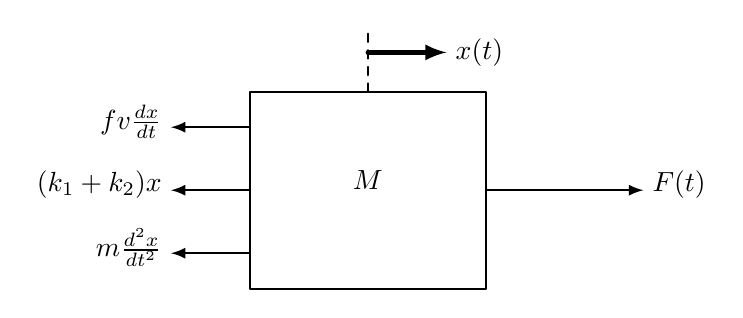
\begin{tikzpicture}[every node/.style={draw,outer sep=0pt,thick}]
			\tikzstyle{spring}=[thick,decorate,decoration={zigzag,pre length=0.1cm,post length=0.1cm,segment length=4}]
			\tikzstyle{damper}=[thick,decoration={markings,
			  mark connection node=dmp,
			  mark=at position 0.5 with
			  {
				\node (dmp) [thick,inner sep=0pt,transform shape,rotate=-90,minimum width=15pt,minimum height=3pt,draw=none] {};
				\draw [thick] ($(dmp.north east)+(2pt,0)$) -- (dmp.south east) -- (dmp.south west) -- ($(dmp.north west)+(2pt,0)$);
				\draw [thick] ($(dmp.north)+(0,-5pt)$) -- ($(dmp.north)+(0,5pt)$);
			  }
			}, decorate]
			\tikzstyle{ground}=[fill,pattern=north east lines,draw=none,minimum width=0.75cm,minimum height=0.3cm]
			
			\begin{scope}[xshift=7cm]
			\node (M) [minimum width=3cm, minimum height=2.5cm, draw, fill=white] {$			\begin{array}{c}

				M\\[5pt]
			\end{array}$};
			\draw [-latex,ultra thick] (M.north) ++(0cm, 0.5cm) -- +(1cm,0cm) node [right,draw=none] (y1) {$x(t)$};
			\draw [dashed] (M.north) -- +(0cm,0.8cm);
			\draw [-latex] (M.east) ++ (0,0) -- +(2cm,0) node[right,yshift=2pt, draw=none] {$F(t)$};
			\draw [-latex] (M.west) ++ (0,0) -- +(-1cm,0) node[left,yshift=2pt, draw=none] {$(k_1+k_2)x$};
			\draw [-latex] (M.west) ++ (0,0.8) -- +(-1cm,0) node[left,yshift=2pt, draw=none] {$fv\frac{dx}{dt}$};
			\draw [-latex] (M.west) ++ (0,-0.8) -- +(-1cm,0) node[left,yshift=2pt, draw=none] {$m\frac{d^2x}{dt^2}$};
			\end{scope}
			\end{tikzpicture}
			\end{center}
\begin{center}
$\sum F_x=0 \quad \rightarrow \quad \oplus$\\[1ex]

$f(t)-m\frac{d^2x}{dt^2}-fv\frac{dx}{dt}-(k_1+k_2)x=0$\\[1ex]

$F(s)-s^2X(s)-2sX(s)-(4+3)X(s)=0$\\[1ex]

$F(s)=(s^2+5s+7)X(s)$\\[1ex]

\boxed{ \dfrac{X(s)}{F(s)} = \dfrac{1}{s^2 + 5s + 7} }
\end{center}

			\clearpage
			\rule{\textwidth}{1pt}
			\textbf{Problem 47}\\
			1. Determine the transfer function $\dfrac{X(s)}{F(s)}$ of the system below\\	

			$K_1 = 2 Nm ; K_2 = 6 Nm ;  fv_1 = 4 Nm/s ;  fv_2 = 2 Nm/s ;  M = 5 kg$\\
			\begin{center}
			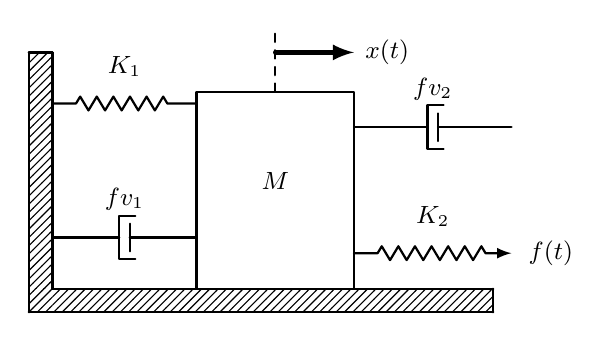
\begin{tikzpicture}
				\tikzstyle{spring}=[thick,decorate,decoration={zigzag,pre length=0.3cm,post length=0.3cm,segment length=6}]
				\tikzstyle{damper}=[thick,decoration={markings,  
				  mark connection node=dmp,
				  mark=at position 0.5 with 
				  {
					\node (dmp) [thick,inner sep=0pt,transform shape,rotate=-90,minimum width=15pt,minimum height=3pt,draw=none] {};
					\draw [thick] ($(dmp.north east)+(2pt,0)$) -- (dmp.south east) -- (dmp.south west) -- ($(dmp.north west)+(2pt,0)$);
					\draw [thick] ($(dmp.north)+(0,-5pt)$) -- ($(dmp.north)+(0,5pt)$);
				  }
				}, decorate]
				\tikzstyle{ground}=[fill,pattern=north east lines,draw=none,minimum width=0.75cm,minimum height=0.3cm,inner sep=0pt,outer sep=0pt]
				
				\node [style={draw,outer sep=0pt,thick}] (M) [minimum width=2cm, minimum height=2.5cm]  {$			\begin{array}{c}
					M\\[5pt]
				\end{array}$};
				\draw [-latex,ultra thick] (M.north) ++(0cm, 0.5cm) -- +(1cm,0cm) node [right,draw=none] (y1) {$x(t)$};
				\draw [dashed] (M.north) -- +(0cm,0.8cm);
				
				\node (ground) [ground,anchor=north,yshift=-0cm,minimum width=5.6cm,xshift=-0.03cm] at (M.south) {};
				\draw (ground.north east) -- (ground.north west);
				\draw (ground.south east) -- (ground.south west);
				\draw (ground.north east) -- (ground.south east);
				
				\node (fill) [ground,xshift=-0.15cm,minimum height = 0.3cm, minimum width = 0.3cm] at (ground.west) {};
				\draw (fill.north west) -- (fill.south west);
				\draw (fill.south west) -- (fill.south east);
				
				
				\node (wall) [ground, rotate=-90, minimum width=3cm,anchor=south east] at (fill.north west) {};
				\draw (wall.north east) -- (wall.north west);
				\draw (wall.north west) -- (wall.south west);
				\draw (wall.south west) -- (wall.south east);
				
				\node (y) at (M.east) [xshift =2.5cm, yshift=-.8cm] {$f(t)$};
				
				\draw [spring] (wall.170) -- ($(M.north west)!(wall.170)!(M.south west)$)node [midway,yshift=6pt, above,draw=none] {$K_1$};
				\draw [damper] (wall.10) -- ($(M.north west)!(wall.10)!(M.south west)$)node [midway,yshift=6pt, above,draw=none] {$fv_1$};;
				
				\draw [-latex,spring] (M.east) ++ (0cm,-.8cm) -- +(2cm,0cm)node [midway,yshift=6pt, above,draw=none] {$K_2$};
				\draw [damper] (M.east) ++ (0cm,.8cm) -- +(2cm,0cm)node [midway,yshift=6pt, above,draw=none] {$fv_2$};
				\end{tikzpicture}
			\end{center}
		\rule{\textwidth}{1pt}

\noindent\textbf{Given:} As per diagram

\vspace{12pt}
\noindent\textit{\textbf{Solution:}}

\vspace{12pt}

		FBD of $M$ \\	
		\begin{center}
			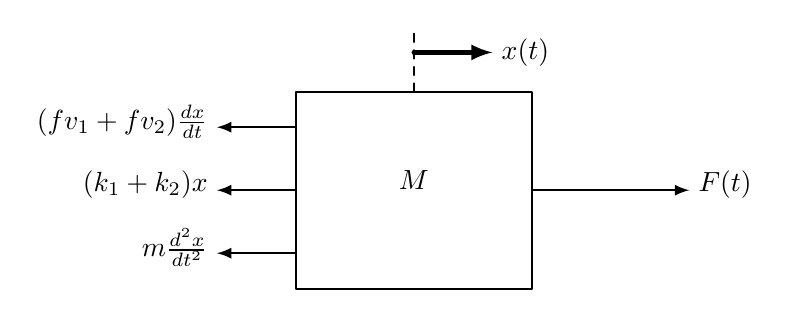
\begin{tikzpicture}[every node/.style={draw,outer sep=0pt,thick}]
			\tikzstyle{spring}=[thick,decorate,decoration={zigzag,pre length=0.1cm,post length=0.1cm,segment length=4}]
			\tikzstyle{damper}=[thick,decoration={markings,
			  mark connection node=dmp,
			  mark=at position 0.5 with
			  {
				\node (dmp) [thick,inner sep=0pt,transform shape,rotate=-90,minimum width=15pt,minimum height=3pt,draw=none] {};
				\draw [thick] ($(dmp.north east)+(2pt,0)$) -- (dmp.south east) -- (dmp.south west) -- ($(dmp.north west)+(2pt,0)$);
				\draw [thick] ($(dmp.north)+(0,-5pt)$) -- ($(dmp.north)+(0,5pt)$);
			  }
			}, decorate]
			\tikzstyle{ground}=[fill,pattern=north east lines,draw=none,minimum width=0.75cm,minimum height=0.3cm]
			
			\begin{scope}[xshift=7cm]
			\node (M) [minimum width=3cm, minimum height=2.5cm, draw, fill=white] {$			\begin{array}{c}
				M\\[5pt]
			\end{array}$};
			\draw [-latex,ultra thick] (M.north) ++(0cm, 0.5cm) -- +(1cm,0cm) node [right,draw=none] (y1) {$x(t)$};
			\draw [dashed] (M.north) -- +(0cm,0.8cm);
			\draw [-latex] (M.east) ++ (0,0) -- +(2cm,0) node[right,yshift=2pt, draw=none] {$F(t)$};
			\draw [-latex] (M.west) ++ (0,0) -- +(-1cm,0) node[left,yshift=2pt, draw=none] {$(k_1+k_2)x$};
			\draw [-latex] (M.west) ++ (0,0.8) -- +(-1cm,0) node[left,yshift=2pt, draw=none] {$(fv_1+fv_2)\frac{dx}{dt}$};
			\draw [-latex] (M.west) ++ (0,-0.8) -- +(-1cm,0) node[left,yshift=2pt, draw=none] {$m\frac{d^2x}{dt^2}$};
			\end{scope}
			\end{tikzpicture}
			\end{center}
\begin{center}
$\sum F_x=0 \quad \rightarrow \quad \oplus$\\[1ex]

$f(t)-m\frac{d^2x}{dt^2}-(fv_1+fv_2)\frac{dx}{dt}-(k_1+k_2)x=0$\\[1ex]

$F(s)-5s^2X(s)-(4+2)sX(s)-(2+6)X(s)=0$\\[1ex]

$F(s)=(5s^2 + 6s + 8)X(s)$\\[1ex]

\boxed{ \dfrac{X(s)}{F(s)} = \dfrac{1}{5s^2 + 6s + 8} }
\end{center}

		
	
\clearpage
\rule{\textwidth}{1pt}
\textbf{Problem 48}\\
Determine the transfer function $\dfrac{X(s)}{F(s)}$ of the system below\\	
\begin{center}
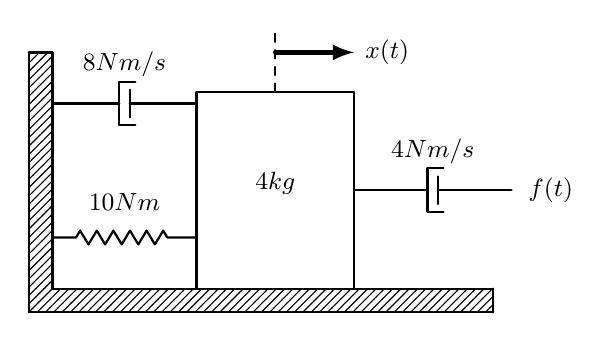
\begin{tikzpicture}
    \tikzstyle{spring}=[thick,decorate,decoration={zigzag,pre length=0.3cm,post length=0.3cm,segment length=6}]
    \tikzstyle{damper}=[thick,decoration={markings,  
        mark connection node=dmp,
        mark=at position 0.5 with 
        {
            \node (dmp) [thick,inner sep=0pt,transform shape,rotate=-90,minimum width=15pt,minimum height=3pt,draw=none] {};
            \draw [thick] ($(dmp.north east)+(2pt,0)$) -- (dmp.south east) -- (dmp.south west) -- ($(dmp.north west)+(2pt,0)$);
            \draw [thick] ($(dmp.north)+(0,-5pt)$) -- ($(dmp.north)+(0,5pt)$);
        }
    }, decorate]
    \tikzstyle{ground}=[fill,pattern=north east lines,draw=none,minimum width=0.75cm,minimum height=0.3cm,inner sep=0pt,outer sep=0pt]
    
    \node [style={draw,outer sep=0pt,thick}] (M) [minimum width=2cm, minimum height=2.5cm]  {$\begin{array}{c}
        4 kg\\[5pt]
    \end{array}$};
    \draw [-latex,ultra thick] (M.north) ++(0cm, 0.5cm) -- +(1cm,0cm) node [right] (y1) {$x(t)$};
    \draw [dashed] (M.north) -- +(0cm,0.8cm);

    \node (ground) [ground,anchor=north,yshift=-0cm,minimum width=5.6cm,xshift=-0.03cm] at (M.south) {};
    \draw (ground.north east) -- (ground.north west);
    \draw (ground.south east) -- (ground.south west);
    \draw (ground.north east) -- (ground.south east);
    
    \node (fill) [ground,xshift=-0.15cm,minimum height = 0.3cm, minimum width = 0.3cm] at (ground.west) {};
    \draw (fill.north west) -- (fill.south west);
    \draw (fill.south west) -- (fill.south east);
    
    \node (wall) [ground, rotate=-90, minimum width=3cm,anchor=south east] at (fill.north west) {};
    \draw (wall.north east) -- (wall.north west);
    \draw (wall.north west) -- (wall.south west);
    \draw (wall.south west) -- (wall.south east);
    
    \node (y) at (M.east) [xshift =2.5cm] {$f(t)$};
    
    \draw [damper] (wall.170) -- ($(M.north west)!(wall.170)!(M.south west)$)node [midway,yshift=6pt, above,draw=none] {$8 Nm/s$};
    \draw [spring] (wall.10) -- ($(M.north west)!(wall.10)!(M.south west)$)node [midway,yshift=6pt, above,draw=none] {$10 Nm$};;
    
    \draw [damper] (M.east) ++ (0cm,0cm) -- +(2cm,0cm) node [midway,yshift=6pt, above,draw=none] {$4 Nm/s$};
\end{tikzpicture}
\end{center}

\rule{\textwidth}{1pt}

\noindent\textbf{Given:} As per diagram

\vspace{12pt}
\noindent\textit{\textbf{Solution:}}

\vspace{12pt}

FBD @ $4kg$ mass\\	
\begin{center}
    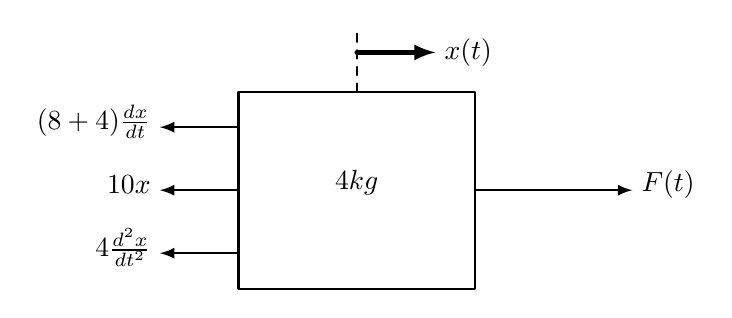
\begin{tikzpicture}[every node/.style={draw,outer sep=0pt,thick}]
    \tikzstyle{spring}=[thick,decorate,decoration={zigzag,pre length=0.1cm,post length=0.1cm,segment length=4}]c
    \tikzstyle{damper}=[thick,decoration={markings,
        mark connection node=dmp,
        mark=at position 0.5 with
        {
            \node (dmp) [thick,inner sep=0pt,transform shape,rotate=-90,minimum width=15pt,minimum height=3pt,draw=none] {};
            \draw [thick] ($(dmp.north east)+(2pt,0)$) -- (dmp.south east) -- (dmp.south west) -- ($(dmp.north west)+(2pt,0)$);
            \draw [thick] ($(dmp.north)+(0,-5pt)$) -- ($(dmp.north)+(0,5pt)$);
        }
    }, decorate]
    \tikzstyle{ground}=[fill,pattern=north east lines,draw=none,minimum width=0.75cm,minimum height=0.3cm]
    
    \begin{scope}[xshift=7cm]
    \node (M) [minimum width=3cm, minimum height=2.5cm, draw, fill=white] {$\begin{array}{c}
        4 kg\\[5pt]
    \end{array}$};

    \draw [-latex,ultra thick] (M.north) ++(0cm, 0.5cm) -- +(1cm,0cm) node [right,draw=none] (y1) {$x(t)$};
    \draw [dashed] (M.north) -- +(0cm,0.8cm);

    \draw [-latex] (M.east) ++ (0,0) -- +(2cm,0) node[right,yshift=2pt, draw=none] {$F(t)$};
    \draw [-latex] (M.west) ++ (0,0) -- +(-1cm,0) node[left,yshift=2pt, draw=none] {$10x$};
    \draw [-latex] (M.west) ++ (0,0.8) -- +(-1cm,0) node[left,yshift=2pt, draw=none] {$(8+4)\frac{dx}{dt}$};
    \draw [-latex] (M.west) ++ (0,-0.8) -- +(-1cm,0) node[left,yshift=2pt, draw=none] {$4\frac{d^2x}{dt^2}$};
    \end{scope}
    \end{tikzpicture}
\end{center}
\begin{center}
$\sum F_x=0 \quad \rightarrow \quad \oplus$\\[1ex]

$f(t) - 4\frac{d^2x}{dt^2} - 12\frac{dx}{dt} - 10x = 0$\\[1ex]

$F(s) - 4s^2X(s) - 12sX(s) - 10X(s) = 0$\\[1ex]

$F(s) = (4s^2 + 12s + 10)X(s)$\\[1ex]

\boxed{ \dfrac{X(s)}{F(s)} = \dfrac{1}{4s^2 + 12s + 10} }
\end{center}


\clearpage
\rule{\textwidth}{1pt}
\textbf{Problem 49}\\
Determine the transfer function $\dfrac{X_2(s)}{F(s)}$ of the system below\\

$K_1 = 3 Nm ; K_2 = 6 Nm ;  fv = 6 Nm/s ;  M_1 = M_2 = 3 kg$\\
\begin{center}
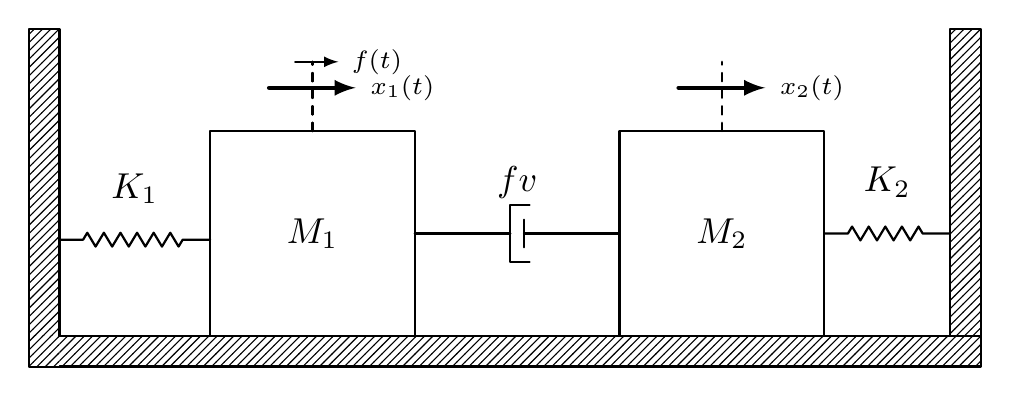
\begin{tikzpicture}[scale=1.1, every node/.style={scale=1.3}]
    \tikzstyle{spring}=[thick,decorate,decoration={zigzag,pre length=0.3cm,post length=0.3cm,segment length=6}]
    \tikzstyle{damper}=[thick,decoration={markings,  
        mark connection node=dmp,
        mark=at position 0.5 with 
        {
            \node (dmp) [thick,inner sep=0pt,transform shape,rotate=-90,minimum width=15pt,minimum height=3pt,draw=none] {};
            \draw [thick] ($(dmp.north east)+(2pt,0)$) -- (dmp.south east) -- (dmp.south west) -- ($(dmp.north west)+(2pt,0)$);
            \draw [thick] ($(dmp.north)+(0,-5pt)$) -- ($(dmp.north)+(0,5pt)$);
        }
    }, decorate]
    \tikzstyle{ground}=[fill,pattern=north east lines,draw=none,minimum width=0.75cm,minimum height=0.3cm,inner sep=0pt,outer sep=0pt]
    
    \node [draw, outer sep=0pt, thick] (M) [minimum width=2cm, minimum height=2cm] {$M_1$};
    \node [draw, outer sep=0pt, thick] (M2) [minimum width=2cm, minimum height=2cm, xshift = 4cm] {$M_2$};
    
    \node (ground) [ground,anchor=north,yshift=-0.0cm,minimum width=9cm,xshift=2.03cm] at (M.south) {};
    \draw (ground.north west) -- (ground.north east) -- (ground.south east) -- (ground.south west);
    
    \node (fill) [ground,xshift=-0.15cm,minimum height = 0.3cm, minimum width = 0.3cm] at (ground.west) {};
    \draw (fill.north west) -- (fill.south west) -- (fill.south east);
    
    \draw [damper] (M.east) -- (M2.west) node (k) [midway,yshift=0.5cm]  {$fv$};
    
    \node (wall) [ground, rotate=-90, minimum width=3cm,anchor=south east] at (fill.north west) {};
    \draw (wall.north east) -- (wall.north west) -- (wall.south west) -- (wall.south east);
    
    \node (wall2) [ground, rotate=-90, minimum width=3cm,anchor=north east,yshift=9cm] at (fill.north east) {};
    \draw (wall2.north east) -- (wall2.north west) -- (wall2.south west) -- (wall2.south east);
    
    \draw [spring] (wall.15) -- ($(M.north west)!(wall.15)!(M.south west)$) node [midway,yshift=0.5cm] {$K_1$};
    
    \draw [spring] (M2.east)-- +(1.45cm,0cm)  node [midway,yshift=0.5cm] {$K_2$};
    
    \draw [-latex,ultra thick] (M.north) ++(-0.5cm, 0.5cm) -- +(1cm,0cm) node [right,draw=none] (y1) {$_{x_1(t)}$};
    \draw [dashed] (M.north) -- +(0cm,0.8cm);

    \draw [-latex] (M.north) ++(-0.2cm, 0.8cm) -- +(.5cm,0cm) node [right,draw=none] (y1) {$_{f(t)}$};
    \draw [dashed] (M.north) -- +(0cm,0.8cm);
    
    \draw [-latex,ultra thick] (M2.north) ++(-0.5cm, 0.5cm) -- +(1cm,0cm) node [right,draw=none] (y1) {$_{x_2(t)}$};
    \draw [dashed](M2.north) -- +(0cm,0.8cm);;
\end{tikzpicture}
\end{center}

\rule{\textwidth}{1pt}

\noindent\textbf{Given:} As per diagram

\vspace{12pt}
\noindent\textit{\textbf{Solution:}}

\vspace{12pt}

\begin{minipage}{.5\textwidth}
\textbf{FBD of $M_1$}\\

$\sum F_x=0 \quad \rightarrow \quad \oplus$\\[1ex]
$f(t) + 6\frac{dx_2}{dt} - 3\frac{d^2x_1}{dt^2} - 6\frac{dx_1}{dt} - 3x_1 = 0$\\[1ex]
$F(s) + 6sX_2(s) - 3s^2X_1(s) - 6sX_1(s) - 3X_1(s) = 0$\\[1ex]
$F(s) = (3s^2 + 6s + 3)X_1(s) - 6sX_2(s) \quad \text{(eq. 1)}$
\vspace{12pt}
\textbf{FBD of $M_2$}\\

$\sum F_x=0 \quad \rightarrow \quad \oplus$\\[1ex]
$6\frac{dx_1}{dt} - 3\frac{d^2x_2}{dt^2} - 6\frac{dx_2}{dt} - 6x_2 = 0$\\[1ex]
$6sX_1(s) - 3s^2X_2(s) - 6sX_2(s) - 6X_2(s) = 0$\\[1ex]
$6sX_1(s) = (3s^2 + 6s + 6)X_2(s)$\\[1ex]
$X_1(s) = \dfrac{3s^2 + 6s + 6}{6s} X_2(s) \quad \text{(eq. 2)}$
\end{minipage}%


\vspace{1.5ex}

Substitute eq. 2 into eq. 1:\\[1ex]
$F(s) = (3s^2 + 6s + 3) \left( \dfrac{3s^2 + 6s + 6}{6s} X_2(s) \right) - 6sX_2(s)$\\[1ex]
$F(s) = X_2(s) \left( \dfrac{(3s^2 + 6s + 3)(3s^2 + 6s + 6)}{6s} - 6s \right)$\\[1ex]
$F(s) = X_2(s) \left( \dfrac{9s^4 + 36s^3 + 63s^2 + 54s + 18 - 36s^2}{6s} \right)$\\[1ex]
$\dfrac{F(s)}{X_2(s)} = \dfrac{9s^4 + 36s^3 + 27s^2 + 54s + 18}{6s}$

\begin{center}
\boxed{ \dfrac{X_2(s)}{F(s)} = \dfrac{6s}{9s^4 + 36s^3 + 27s^2 + 54s + 18} }
\end{center}

\clearpage
\rule{\textwidth}{1pt}
\textbf{Problem 50}\\
Determine the transfer function $\dfrac{X_2(s)}{F(s)}$ of the system below\\
\begin{center}
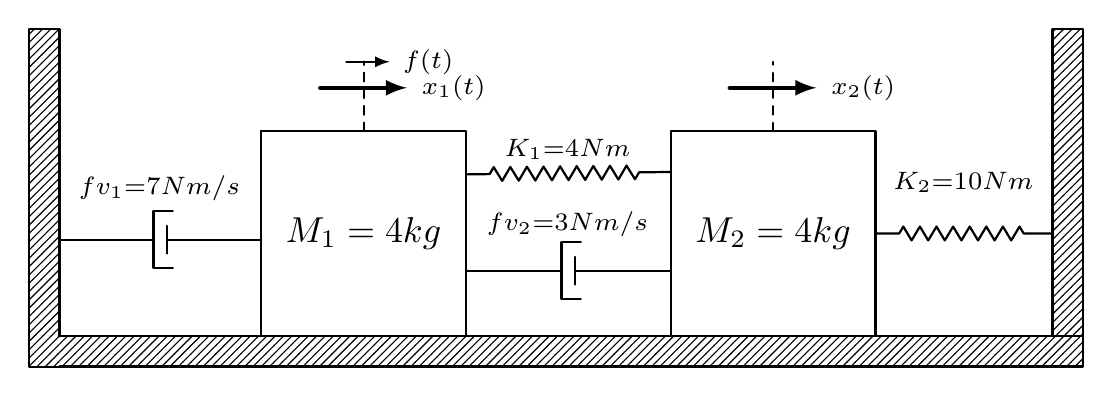
\begin{tikzpicture}[scale=1.1, every node/.style={scale=1.3}]
    \tikzstyle{spring}=[thick,decorate,decoration={zigzag,pre length=0.3cm,post length=0.3cm,segment length=6}]
    \tikzstyle{damper}=[thick,decoration={markings,  
        mark connection node=dmp,
        mark=at position 0.5 with 
        {
            \node (dmp) [thick,inner sep=0pt,transform shape,rotate=-90,minimum width=15pt,minimum height=3pt,draw=none] {};
            \draw [thick] ($(dmp.north east)+(2pt,0)$) -- (dmp.south east) -- (dmp.south west) -- ($(dmp.north west)+(2pt,0)$);
            \draw [thick] ($(dmp.north)+(0,-5pt)$) -- ($(dmp.north)+(0,5pt)$);
        }
    }, decorate]
    \tikzstyle{ground}=[fill,pattern=north east lines,draw=none,minimum width=0.75cm,minimum height=0.3cm,inner sep=0pt,outer sep=0pt]
    
    \node [draw, outer sep=0pt, thick] (M) [minimum width=2cm, minimum height=2cm] {$M_1=4 kg$};
    \node [draw, outer sep=0pt, thick] (M2) [minimum width=2cm, minimum height=2cm, xshift = 4cm] {$M_2=4 kg$};
    
    \node (ground) [ground,anchor=north,yshift=-0.0cm,minimum width=10cm,xshift=2.03cm] at (M.south) {};
    \draw (ground.north west) -- (ground.north east) -- (ground.south east) -- (ground.south west);
    
    \node (fill) [ground,xshift=-0.15cm,minimum height = 0.3cm, minimum width = 0.3cm] at (ground.west) {};
    \draw (fill.north west) -- (fill.south west) -- (fill.south east);
    
    \draw [spring] (M.30) -- (M2.-211) node (k) [midway,above] {$_{K_1=4 Nm}$};
    \draw [damper] (M.-20) -- (M2.-160) node (k) [midway,above,yshift=0.2cm] {$ _{fv_2=3 Nm/s}$};
    
    \node (wall) [ground, rotate=-90, minimum width=3cm,anchor=south east] at (fill.north west) {};
    \draw (wall.north east) -- (wall.north west) -- (wall.south west) -- (wall.south east);
    
    \node (wall2) [ground, rotate=-90, minimum width=3cm,anchor=north east,yshift=10cm] at (fill.north east) {};
    \draw (wall2.north east) -- (wall2.north west) -- (wall2.south west) -- (wall2.south east);
    
    \draw [damper] (wall.15) -- ($(M.north west)!(wall.15)!(M.south west)$) node [midway,yshift=0.5cm] {$ _{fv_1=7 Nm/s}$};
    
    \draw [spring] (M2.east)-- +(2.05cm,0cm)  node [midway,yshift=0.5cm] {$_{K_2=10 Nm}$};
    
    \draw [-latex,ultra thick] (M.north) ++(-0.5cm, 0.5cm) -- +(1cm,0cm) node [right,draw=none] (y1) {$_{x_1(t)}$};
    \draw [dashed] (M.north) -- +(0cm,0.8cm);

    \draw [-latex] (M.north) ++(-0.2cm, 0.8cm) -- +(.5cm,0cm) node [right,draw=none] (y1) {$_{f(t)}$};
    \draw [dashed] (M.north) -- +(0cm,0.8cm);
    
    \draw [-latex,ultra thick] (M2.north) ++(-0.5cm, 0.5cm) -- +(1cm,0cm) node [right,draw=none] (y1) {$_{x_2(t)}$};
    \draw [dashed](M2.north) -- +(0cm,0.8cm);;
\end{tikzpicture}
\end{center}

\rule{\textwidth}{1pt}

\noindent\textbf{Given:} As per diagram

\vspace{12pt}
\noindent\textit{\textbf{Solution:}}

\vspace{12pt}

\begin{center}

FBD of $M_1$\\

$\sum F_x=0 \quad \rightarrow \quad \oplus$\\

$f(t)+3\frac{dx_2}{dt}+4x_2-4\frac{d^2x_1}{dt^2}-10\frac{dx_1}{dt}-4x_1=0$\\

$F(s)+3sX_2(s)+4X_2(s)-4s^2X_1(s)-10sX_1(s)-4X_1(s)=0$\\

$F(s)=(4s^2+10s+4)X_1(s)-(3s+4)X_2(s) \rightarrow \text{eq.1}$\\

FBD of $M_2$\\

$\sum F_x=0 \quad \rightarrow \quad \oplus$\\

$3\frac{dx_1}{dt}+4x_1-4\frac{d^2x_2}{dt^2}-3\frac{dx_2}{dt}-14x_2=0$\\

$3sX_1(s)+4X_1(s)-4s^2X_2(s)-3sX_2(s)-14X_2(s)=0$\\

$(3s+4)X_1(s)=(4s^2+3s+14)X_2(s)$\\

$X_1(s)=\dfrac{4s^2+3s+14}{3s+4}X_2(s) \rightarrow \text{eq.2}$\\

Substitute eq.2 to eq.1\\

$F(s)=(4s^2+10s+4)\left(\dfrac{4s^2+3s+14}{3s+4}X_2(s)\right)-(3s+4)X_2(s)$\\

$F(s)=X_2(s)\left(\dfrac{16s^4+52s^3+93s^2+138s+40}{3s+4}\right)$\\

$\dfrac{F(s)}{X_2(s)}=\dfrac{16s^4+52s^3+93s^2+138s+40}{3s+4}$\\

\boxed{ \dfrac{X_2(s)}{F(s)} = \dfrac{3s+4}{16s^4 + 52s^3 + 93s^2 + 138s + 40} }

\end{center}




\clearpage
\rule{\textwidth}{1pt}
\textbf{Problem 51}\\
1. Determine the transfer function $\dfrac{\theta(s)}{T(s)}$ of the system below\\
\tdplotsetmaincoords{60}{110}
\begin{center}
\begin{tikzpicture}[scale=1.1,tdplot_main_coords,every node/.style={draw,outer sep=0pt,thick}]
    \tikzstyle{spring}=[thick,decorate,decoration={zigzag,pre length=0.1cm,post length=0.1cm,segment length=4}]
    \tikzstyle{damper}=[thick,decoration={markings,
      mark connection node=dmp,
      mark=at position 0.5 with
      {
        \node (dmp) [thick,inner sep=0pt,transform shape,rotate=-90,minimum width=15pt,minimum height=3pt,draw=none] {};
        \draw [thick] ($(dmp.north east)+(2pt,0)$) -- (dmp.south east) -- (dmp.south west) -- ($(dmp.north west)+(2pt,0)$);
        \draw [thick] ($(dmp.north)+(0,-5pt)$) -- ($(dmp.north)+(0,5pt)$);
      }
    }, decorate]
    \tikzstyle{ground}=[fill,pattern=north east lines,draw=none,minimum width=0.75cm,minimum height=0.3cm]
    \begin{scope}[shift={(8.,0)}]
        \node(J)[cylinder, draw, shape aspect=.5,
           cylinder uses custom fill, cylinder end fill=white,
            minimum height=1cm,
        cylinder body fill=white, opacity=1,
        scale=3, rotate=180]{};

        
        \node (wall) [ground, rotate=-90, minimum width=3cm,yshift=-4cm] {};
        \draw (wall.north east) -- (wall.north west);

        \node (wall2) [ground, rotate=90, minimum width=3cm,yshift=-3.1cm] {};
        \draw (wall2.north east) -- (wall2.north west);
    
        \draw [damper] (wall.100) -- (J.east) node[midway,yshift=10pt, above ,draw=none] {$_{5 N-m-s/rad}$};
    
        \draw [spring] (J.west) ++ (0,0) -- +(1.5cm,0) node [midway,yshift=6pt, above,draw=none] {$_{9 N-m/rad}$};
    
        % Add text inside the cylinder
        \node[anchor=center, yshift=0.1cm, draw=none] at (J.center) {$_{6 kg-m^2}$};
    \end{scope}
    \tdplotsetthetaplanecoords{180}

    \tdplotdrawarc[tdplot_rotated_coords,->,color=black]{(0,-7.8,0)}{0.6}{165}{450}{anchor=south west,yshift=.5cm,xshift=0cm,color=black,draw=none}{$_{T(t)}$}
    \tdplotdrawarc[tdplot_rotated_coords,->,color=black]{(0,-8.2,1)}{0.6}{165}{450}{anchor=south west,yshift=.5cm,xshift=0cm,color=black,draw=none}{$_{\theta (t)}$}

\end{tikzpicture}
\end{center}

\rule{\textwidth}{1pt}

\noindent\textbf{Given:} As per diagram

\vspace{12pt}
\noindent\textit{\textbf{Solution:}}

\vspace{12pt}

\begin{center}

\vspace{12pt}

FBD @ 6 $kg\text{-}m^2$ inertia\\

\begin{tikzpicture}
    \draw[] (0,0) circle (2cm) ;
    \node at (0,0) {$6 kg\text{-}m^2$};
    \draw[-{Latex[length=2mm]}, thick, bend left=45, shorten >=5pt] (70:2.2cm) to[bend left=35]  node[midway, left, yshift=.5cm]{$T(t)$} (25:2.2cm);
    \draw[-{Latex[length=2mm]}, thick, bend right=45, shorten >=5pt] (105:2.2cm) to[bend right=35] node[midway, left, yshift=.3cm] {$9 \theta(t) $} (150:2.2cm);
    \draw[-{Latex[length=2mm]}, thick, bend right=45, shorten >=5pt] (155:2.2cm) to[bend right=35] node[midway, left] {$5\dfrac{d\theta(t)}{dt}$} (200:2.2cm);
    \draw[-{Latex[length=2mm]}, thick, bend right=45, shorten >=5pt] 
      (205:2.2cm) to[bend right=35] node[midway, below,xshift=-.5cm] {$6\dfrac{d^2\theta(t)}{dt^2}$} (250:2.2cm);
\end{tikzpicture}

$\sum T = 0 \quad \circlearrowright \hspace{-0.8em} $+$  $ \\

$T(t)-6\dfrac{d^2\theta(t)}{dt^2}-5\dfrac{d\theta(t)}{dt}-9 \theta(t)=0$\\

$T(s)-6s^2\theta(s)-5s\theta(s)-9\theta(s)=0$\\

$(6s^2+5s+9)\theta(s)=T(s)$\\

$\dfrac{T(s)}{\theta(s)}=(6s^2+5s+9)$\\

\boxed{ \dfrac{\theta(s)}{T(s)}=\dfrac{1}{6s^2+5s+9} }

\end{center}



    

\clearpage
\rule{\textwidth}{1pt}
\textbf{Problem 52}\\
1. Determine the transfer function $\dfrac{\theta(s)}{T(s)}$ of the system below\\

$D=3N-m-s/rad ; K_1=4 N-m/rad ; K_2=5 N-m/rad ; J=6 kg-m^2$\\
\tdplotsetmaincoords{60}{110}
\begin{center}
\begin{tikzpicture}[scale=1.1,tdplot_main_coords,every node/.style={draw,outer sep=0pt,thick}]
    \tikzstyle{spring}=[thick,decorate,decoration={zigzag,pre length=0.1cm,post length=0.1cm,segment length=4}]
    \tikzstyle{damper}=[thick,decoration={markings,
      mark connection node=dmp,
      mark=at position 0.5 with
      {
        \node (dmp) [thick,inner sep=0pt,transform shape,rotate=-90,minimum width=15pt,minimum height=3pt,draw=none] {};
        \draw [thick] ($(dmp.north east)+(2pt,0)$) -- (dmp.south east) -- (dmp.south west) -- ($(dmp.north west)+(2pt,0)$);
        \draw [thick] ($(dmp.north)+(0,-5pt)$) -- ($(dmp.north)+(0,5pt)$);
      }
    }, decorate]
    \tikzstyle{ground}=[fill,pattern=north east lines,draw=none,minimum width=0.75cm,minimum height=0.3cm]
    \begin{scope}[shift={(8.,0)}]
        \node(J)[cylinder, draw, shape aspect=.5,
           cylinder uses custom fill, cylinder end fill=white,
            minimum height=1cm,
        cylinder body fill=white, opacity=1,
        scale=3, rotate=180]{};

        
        \node (wall) [ground, rotate=-90, minimum width=3cm,yshift=-3cm] {};
        \draw (wall.north east) -- (wall.north west);

        \node (wall2) [ground, rotate=90, minimum width=3cm,yshift=-3.1cm] {};
        \draw (wall2.north east) -- (wall2.north west);
    
        \draw [damper] (wall.148) -- (J.-8) node[midway,yshift=10pt, above ,draw=none] {$D$};

        \draw [spring] (wall.30) -- (J.8) node[midway, below ,draw=none] {$K_1$};
    
        \draw [spring] (J.west) ++ (0,0) -- +(1.5cm,0) node [midway,yshift=6pt, above,draw=none] {$K_2$};
    
        % Add text inside the cylinder
        \node[anchor=center, yshift=0.1cm, draw=none] at (J.center) {J};
    \end{scope}
    \tdplotsetthetaplanecoords{180}

    \tdplotdrawarc[tdplot_rotated_coords,->,color=black]{(0,-7.8,0)}{0.6}{165}{450}{anchor=south west,yshift=.5cm,xshift=0cm,color=black,draw=none}{$_{T(t)}$}
    \tdplotdrawarc[tdplot_rotated_coords,->,color=black]{(0,-8.2,1)}{0.6}{165}{450}{anchor=south west,yshift=.5cm,xshift=0cm,color=black,draw=none}{$_{\theta (t)}$}

\end{tikzpicture}
\end{center}

\rule{\textwidth}{1pt}

\noindent\textbf{Given:} As per diagram

\vspace{12pt}
\begin{center}
\noindent\textit{\textbf{Solution:}}
\vspace{12pt}

FBD of J inertia\\

\begin{tikzpicture}
    \draw[] (0,0) circle (2cm) ;
    \node at (0,0) {$J$};
    \draw[-{Latex[length=2mm]}, thick, bend left=45, shorten >=5pt] (70:2.2cm) to[bend left=35]  node[midway, left, yshift=.5cm]{$T(t)$} (25:2.2cm);
    \draw[-{Latex[length=2mm]}, thick, bend right=45, shorten >=5pt] (105:2.2cm) to[bend right=35] node[midway, left, yshift=.3cm] {$(4+5) \theta(t) $} (150:2.2cm);
    \draw[-{Latex[length=2mm]}, thick, bend right=45, shorten >=5pt] (155:2.2cm) to[bend right=35] node[midway, left] {$3\dfrac{d\theta(t)}{dt}$} (200:2.2cm);
    \draw[-{Latex[length=2mm]}, thick, bend right=45, shorten >=5pt] 
      (205:2.2cm) to[bend right=35] node[midway, below,xshift=-.5cm] {$6\dfrac{d^2\theta(t)}{dt^2}$} (250:2.2cm);
    \end{tikzpicture}

    $\sum T = 0 \quad \circlearrowright \hspace{-0.8em} $+$  $ \\

    $T(t)-6\dfrac{d^2\theta(t)}{dt^2}-3\dfrac{d\theta(t)}{dt}-(4+5) \theta(t)=0$\\

    $T(s)-6s^2\theta(s)-3s\theta(s)-9\theta(s)=0$\\

    $(6s^2+3s+9)\theta(s)=T(s)$\\

    $\dfrac{T(s)}{\theta(s)}=(6s^2+3s+9)$\\

	
    \boxed{ \begin{aligned} & \dfrac{\theta(s)}{T(s)}=\dfrac{1}{6s^2+3s+9} \ \end{aligned} }


\end{center}
			\clearpage
			\rule{\textwidth}{1pt}
			\textbf{Problem 53}\\
			1. Determine the transfer function $\dfrac{\theta(s)}{T(s)}$ of the system below\\
			
			$D_1=9N-m-s/rad ; D_2=4N-m-s/rad ; K=5 N-m/rad ; J=3 kg-m^2$\\
			\tdplotsetmaincoords{60}{110}
			\begin{center}
			\begin{tikzpicture}[scale=1.1,tdplot_main_coords,every node/.style={draw,outer sep=0pt,thick}]
				\tikzstyle{spring}=[thick,decorate,decoration={zigzag,pre length=0.1cm,post length=0.1cm,segment length=4}]
				\tikzstyle{damper}=[thick,decoration={markings,
				  mark connection node=dmp,
				  mark=at position 0.5 with
				  {
					\node (dmp) [thick,inner sep=0pt,transform shape,rotate=-90,minimum width=15pt,minimum height=3pt,draw=none] {};
					\draw [thick] ($(dmp.north east)+(2pt,0)$) -- (dmp.south east) -- (dmp.south west) -- ($(dmp.north west)+(2pt,0)$);
					\draw [thick] ($(dmp.north)+(0,-5pt)$) -- ($(dmp.north)+(0,5pt)$);
				  }
				}, decorate]
				\tikzstyle{ground}=[fill,pattern=north east lines,draw=none,minimum width=0.75cm,minimum height=0.3cm]
				\begin{scope}[shift={(8.,0)}]
					\node(J)[cylinder, draw, shape aspect=.5,
 				   cylinder uses custom fill, cylinder end fill=white,
    				minimum height=1cm,
    			cylinder body fill=white, opacity=1,
    			scale=3, rotate=180]{};

				
					\node (wall) [ground, rotate=-90, minimum width=3cm,yshift=-3cm] {};
					\draw (wall.north east) -- (wall.north west);

					\node (wall2) [ground, rotate=90, minimum width=3cm,yshift=-3.1cm] {};
					\draw (wall2.north east) -- (wall2.north west);
				
					\draw [damper] (wall.148) -- (J.-8) node[midway,yshift=10pt, above ,draw=none] {$D_1$};

					\draw [spring] (wall.30) -- (J.8) node[midway, below ,draw=none] {$K$};
				
					\draw [damper] (J.west) ++ (0,0) -- +(1.5cm,0) node [midway,yshift=6pt, above,draw=none] {$D_2$};
				
					% Add text inside the cylinder
					\node[anchor=center, yshift=0.1cm, draw=none] at (J.center) {J};
				\end{scope}
				\tdplotsetthetaplanecoords{180}
		
				\tdplotdrawarc[tdplot_rotated_coords,->,color=black]{(0,-7.8,0)}{0.6}{165}{450}{anchor=south west,yshift=.5cm,xshift=0cm,color=black,draw=none}{$_{T(t)}$}
				\tdplotdrawarc[tdplot_rotated_coords,->,color=black]{(0,-8.2,1)}{0.6}{165}{450}{anchor=south west,yshift=.5cm,xshift=0cm,color=black,draw=none}{$_{\theta (t)}$}
			
			\end{tikzpicture}
		\end{center}

			\rule{\textwidth}{1pt}

\noindent\textbf{Given:} As per diagram

\vspace{12pt}
\noindent\textit{\textbf{Solution:}}

\begin{center}

\vspace{12pt}

			FBD of J inertia\\
			
			\begin{tikzpicture}
				\draw[] (0,0) circle (2cm) ;
				\node at (0,0) {$J$};
				\draw[-{Latex[length=2mm]}, thick, bend left=45, shorten >=5pt] (70:2.2cm) to[bend left=35]  node[midway, left, yshift=.5cm]{$T(t)$} (25:2.2cm);
				\draw[-{Latex[length=2mm]}, thick, bend right=45, shorten >=5pt] (105:2.2cm) to[bend right=35] node[midway, left, yshift=.3cm] {$5 \theta(t) $} (150:2.2cm);
				\draw[-{Latex[length=2mm]}, thick, bend right=45, shorten >=5pt] (155:2.2cm) to[bend right=35] node[midway, left] {$(9+4)\dfrac{d\theta(t)}{dt}$} (200:2.2cm);
				\draw[-{Latex[length=2mm]}, thick, bend right=45, shorten >=5pt] 
 				 (205:2.2cm) to[bend right=35] node[midway, below,xshift=-.5cm] {$3\dfrac{d^2\theta(t)}{dt^2}$} (250:2.2cm);
				\end{tikzpicture}

				$\sum T = 0 \quad \circlearrowright \hspace{-0.8em} $+$  $ \\

				$T(t)-3\dfrac{d^2\theta(t)}{dt^2}-(9+4)\dfrac{d\theta(t)}{dt}-5\theta(t)=0$\\

				$T(s)-3s^2\theta(s)-13s\theta(s)-5\theta(s)=0$\\

				$(3s^2+13s+5)\theta(s)=T(s)$\\

				$\dfrac{T(s)}{\theta(s)}=(3s^2+13s+5)$\\
	\begin{center}
\boxed{ \begin{aligned} & \dfrac{\theta(s)}{T(s)}=\dfrac{1}{3s^2+13s+5} \ \end{aligned} }
\end{center}

\end{center}			
			

			\clearpage
			\rule{\textwidth}{1pt}
			\textbf{Problem 54}\\
			1. Determine the transfer function $\dfrac{\theta_1(s)}{T(s)}$ of the system below\\

			$D=2N-m-s/rad ; K_1=3N-m/rad ; K_2=6 N-m/rad ; J1=J2=5 kg-m^2$\\
			\tdplotsetmaincoords{60}{110}
			\begin{center}
			\begin{tikzpicture}[scale=1.1,tdplot_main_coords,every node/.style={draw,outer sep=0pt,thick}]
				\tikzstyle{spring}=[thick,decorate,decoration={zigzag,pre length=0.1cm,post length=0.1cm,segment length=4}]
				\tikzstyle{damper}=[thick,decoration={markings,
				  mark connection node=dmp,
				  mark=at position 0.5 with
				  {
					\node (dmp) [thick,inner sep=0pt,transform shape,rotate=-90,minimum width=15pt,minimum height=3pt,draw=none] {};
					\draw [thick] ($(dmp.north east)+(2pt,0)$) -- (dmp.south east) -- (dmp.south west) -- ($(dmp.north west)+(2pt,0)$);
					\draw [thick] ($(dmp.north)+(0,-5pt)$) -- ($(dmp.north)+(0,5pt)$);
				  }
				}, decorate]
				\tikzstyle{ground}=[fill,pattern=north east lines,draw=none,minimum width=0.75cm,minimum height=0.3cm]
				\begin{scope}[shift={(8.,0)}]
					\node(J)[cylinder, draw, shape aspect=.5,
 				   cylinder uses custom fill, cylinder end fill=white,
    				minimum height=1cm,
    			cylinder body fill=white, opacity=1,
    			scale=3, rotate=180]{};

				\node(J1)[cylinder, draw, shape aspect=.5,
 				   cylinder uses custom fill, cylinder end fill=white,
    				minimum height=1cm,
    			cylinder body fill=white, opacity=1,
    			scale=3, rotate=180, xshift=-1.5cm]{};

				
					\node (wall) [ground, rotate=-90, minimum width=3cm,yshift=-3.5cm] {};
					\draw (wall.north east) -- (wall.north west);

					\node (wall2) [ground, rotate=90, minimum width=3cm,yshift=-7.5cm] {};
					\draw (wall2.north east) -- (wall2.north west);
			

					\draw [spring] (wall.100) -- (J.east) node[midway, below ,draw=none] {$K_1$};
				
					\draw [damper] (J.west) -- (J1.east) node [midway,yshift=6pt, above,draw=none] {$D$};
					
					\draw [spring] (J1.west) ++ (0,0) -- +(1.4cm,0) node [midway,yshift=6pt, above,draw=none] {$K_2$};
				
					% Add text inside the cylinder
					\node[anchor=center, yshift=0.1cm, draw=none] at (J.center) {J1};
					\node[anchor=center, yshift=0.1cm, draw=none] at (J1.center) {J2};
				\end{scope}
				\tdplotsetthetaplanecoords{180}
		
				\tdplotdrawarc[tdplot_rotated_coords,->,color=black]{(0,-7.8,0)}{0.6}{165}{450}{anchor=south west,yshift=.5cm,xshift=0cm,color=black,draw=none}{$_{T(t)}$}
				\tdplotdrawarc[tdplot_rotated_coords,->,color=black]{(0,-8.2,1)}{0.6}{165}{450}{anchor=south west,yshift=.5cm,xshift=0cm,color=black,draw=none}{$_{\theta_1 (t)}$}
			
				\tdplotdrawarc[tdplot_rotated_coords,->,color=black]{(0,-6.4,-4)}{0.6}{165}{450}{anchor=south west,yshift=.5cm,xshift=0cm,color=black,draw=none}{$_{\theta_2 (t)}$}

			\end{tikzpicture}
		\end{center}

			\rule{\textwidth}{1pt}

\noindent\textbf{Given:} As per diagram

\vspace{12pt}
\noindent\textit{\textbf{Solution:}}
\begin{center}

\vspace{12pt}

			\begin{minipage}{.5\textwidth}
				FBD of J1 inertia\\
				\begin{tikzpicture}
					\draw[] (0,0) circle (2cm) ;
					\node at (0,0) {$J1$};
					\draw[-{Latex[length=2mm]}, thick, bend left=45, shorten >=5pt] (70:2.2cm) to[bend left=35]  node[midway, left, yshift=.5cm]{$T(t)$} (25:2.2cm);
					\draw[-{Latex[length=2mm]}, thick, bend left=45, shorten >=5pt] (25:2.2cm) to[bend left=30]  node[midway, right, yshift=.5cm]{$2\dfrac{d\theta_2(t)}{dt}$} (340:2.2cm);
					\draw[-{Latex[length=2mm]}, thick, bend right=45, shorten >=5pt] (105:2.2cm) to[bend right=35] node[midway, left, yshift=.3cm] {$3 \theta_1(t) $} (150:2.2cm);
					\draw[-{Latex[length=2mm]}, thick, bend right=45, shorten >=5pt] (155:2.2cm) to[bend right=35] node[midway, left] {$2\dfrac{d\theta_1(t)}{dt}$} (200:2.2cm);
					\draw[-{Latex[length=2mm]}, thick, bend right=45, shorten >=5pt] 
					  (205:2.2cm) to[bend right=35] node[midway, below,xshift=-.5cm] {$3\dfrac{d^2\theta_1(t)}{dt^2}$} (250:2.2cm);
					\end{tikzpicture}
	
					$\sum T = 0 \quad \circlearrowright \hspace{-0.8em} $+$  $ \\
	
					$T(t)+2\dfrac{d\theta_2(t)}{dt}-5\dfrac{d^2\theta_1(t)}{dt^2}-2\dfrac{d\theta_1(t)}{dt}-3\theta_1(t)=0$\\
	
					$T(s)+2s\theta_2(s)-5s^2\theta_1(s)-2s\theta_1(s)-3\theta_1(s)=0$\\
	
					$(5s^2+2s+3)\theta_1(s)-2s\theta_2(s)=T(s) \rightarrow eq.1 $\\
			\end{minipage}		

			\newpage	

\begin{minipage}{.5\textwidth}
FBD of $J_2$ inertia:
\vspace{4pt}

\begin{tikzpicture}
	\draw[] (0,0) circle (2cm);
	\node at (0,0) {$J_2$};
	\draw[-{Latex[length=2mm]}, thick, bend left=45, shorten >=5pt] (70:2.2cm) to[bend left=35]  node[midway, right, yshift=.5cm]{$2\dfrac{d\theta_1(t)}{dt}$} (25:2.2cm);
	\draw[-{Latex[length=2mm]}, thick, bend right=45, shorten >=5pt] (105:2.2cm) to[bend right=35] node[midway, left, yshift=.3cm] {$6 \theta_2(t)$} (150:2.2cm);
	\draw[-{Latex[length=2mm]}, thick, bend right=45, shorten >=5pt] (155:2.2cm) to[bend right=35] node[midway, left] {$2\dfrac{d\theta_2(t)}{dt}$} (200:2.2cm);
	\draw[-{Latex[length=2mm]}, thick, bend right=45, shorten >=5pt] (205:2.2cm) to[bend right=35] node[midway, below,xshift=-.5cm] {$5\dfrac{d^2\theta_2(t)}{dt^2}$} (250:2.2cm);
\end{tikzpicture}

\vspace{4pt}
$\sum T = 0 \quad \circlearrowright +$\\

$2\dfrac{d\theta_1(t)}{dt} - 5\dfrac{d^2\theta_2(t)}{dt^2} - 2\dfrac{d\theta_2(t)}{dt} - 6\theta_2(t) = 0$\\

$2s\theta_1(s) - 5s^2\theta_2(s) - 2s\theta_2(s) - 6\theta_2(s) = 0$\\

$2s\theta_1(s) = (5s^2 + 2s + 6)\theta_2(s)$\\

$\theta_2(s) = \dfrac{2s}{5s^2 + 2s + 6}\theta_1(s) \quad \text{(eq. 2)}$\\
\end{minipage}

\vspace{1em}

Substitute eq. 2 into the torque equation:

\[
(5s^2 + 2s + 3)\theta_1(s) - 2s\theta_2(s) = T(s)
\]

\[
(5s^2 + 2s + 3)\theta_1(s) - 2s\left(\dfrac{2s}{5s^2 + 2s + 6}\theta_1(s)\right) = T(s)
\]

\[
\Rightarrow \theta_1(s) \left( (5s^2 + 2s + 3) - \dfrac{4s^2}{5s^2 + 2s + 6} \right) = T(s)
\]

\[
\Rightarrow \dfrac{T(s)}{\theta_1(s)} = \dfrac{25s^4 + 20s^3 + 30s^2 + 12s + 9}{5s^2 + 2s + 6}
\]

\begin{center}
\boxed{ \dfrac{\theta_1(s)}{T(s)} = \dfrac{5s^2 + 2s + 6}{25s^4 + 20s^3 + 30s^2 + 12s + 9} }
\end{center}

\end{center}

			\clearpage
			\rule{\textwidth}{1pt}
			\textbf{Problem 55}\\
			1. Determine the transfer function $\dfrac{\theta_1(s)}{T(s)}$ of the system below\\
			$D=8N-m-s/rad ; K_1=5N-m/rad ; K_2=K_3=7 N-m/rad ; J1=J2=7 kg-m^2$\\
			\tdplotsetmaincoords{60}{110}
			\begin{center}
			\begin{tikzpicture}[scale=1.1,tdplot_main_coords,every node/.style={draw,outer sep=0pt,thick}]
				\tikzstyle{spring}=[thick,decorate,decoration={zigzag,pre length=0.1cm,post length=0.1cm,segment length=4}]
				\tikzstyle{damper}=[thick,decoration={markings,
				  mark connection node=dmp,
				  mark=at position 0.5 with
				  {
					\node (dmp) [thick,inner sep=0pt,transform shape,rotate=-90,minimum width=15pt,minimum height=3pt,draw=none] {};
					\draw [thick] ($(dmp.north east)+(2pt,0)$) -- (dmp.south east) -- (dmp.south west) -- ($(dmp.north west)+(2pt,0)$);
					\draw [thick] ($(dmp.north)+(0,-5pt)$) -- ($(dmp.north)+(0,5pt)$);
				  }
				}, decorate]
				\tikzstyle{ground}=[fill,pattern=north east lines,draw=none,minimum width=0.75cm,minimum height=0.3cm]
				\begin{scope}[shift={(8.,0)}]
					\node(J)[cylinder, draw, shape aspect=.5,
 				   cylinder uses custom fill, cylinder end fill=white,
    				minimum height=1cm,
    			cylinder body fill=white, opacity=1,
    			scale=3, rotate=180]{};

				\node(J1)[cylinder, draw, shape aspect=.5,
 				   cylinder uses custom fill, cylinder end fill=white,
    				minimum height=1cm,
    			cylinder body fill=white, opacity=1,
    			scale=3, rotate=180, xshift=-1.5cm]{};

				
					\node (wall) [ground, rotate=-90, minimum width=3cm,yshift=-3.5cm] {};
					\draw (wall.north east) -- (wall.north west);

					\node (wall2) [ground, rotate=90, minimum width=3cm,yshift=-7.5cm] {};
					\draw (wall2.north east) -- (wall2.north west);
			

					\draw [spring] (wall.100) -- (J.east) node[midway, below ,draw=none] {$K_1$};
				
					\draw [damper] (J.910) -- (J1.-8) node [midway,yshift=6pt, above,draw=none] {$D$};
					\draw [spring] (J.890) -- (J1.8) node [midway, below,draw=none] {$K_2$};
					
					\draw [spring] (J1.west) ++ (0,0) -- +(1.4cm,0) node [midway,yshift=6pt, above,draw=none] {$K_3$};
				
					% Add text inside the cylinder
					\node[anchor=center, yshift=0.1cm, draw=none] at (J.center) {J1};
					\node[anchor=center, yshift=0.1cm, draw=none] at (J1.center) {J2};
				\end{scope}
				\tdplotsetthetaplanecoords{180}
		
				\tdplotdrawarc[tdplot_rotated_coords,->,color=black]{(0,-7.8,0)}{0.6}{165}{450}{anchor=south west,yshift=.5cm,xshift=0cm,color=black,draw=none}{$_{T(t)}$}
				\tdplotdrawarc[tdplot_rotated_coords,->,color=black]{(0,-8.2,1)}{0.6}{165}{450}{anchor=south west,yshift=.5cm,xshift=0cm,color=black,draw=none}{$_{\theta_1 (t)}$}
			
				\tdplotdrawarc[tdplot_rotated_coords,->,color=black]{(0,-6.4,-4)}{0.6}{165}{450}{anchor=south west,yshift=.5cm,xshift=0cm,color=black,draw=none}{$_{\theta_2 (t)}$}

			\end{tikzpicture}
		\end{center}

			\rule{\textwidth}{1pt}

\noindent\textbf{Given:} As per diagram

\vspace{12pt}
\noindent\textit{\textbf{Solution:}}
\begin{center}
\vspace{12pt}

			\begin{minipage}{.5\textwidth}
				FBD of J1 inertia\\
				\begin{tikzpicture}
					\draw[] (0,0) circle (2cm) ;
					\node at (0,0) {$J1$};
					\draw[-{Latex[length=2mm]}, thick, bend left=45, shorten >=5pt] (70:2.2cm) to[bend left=35]  node[midway, left, yshift=.5cm]{$T(t)$} (25:2.2cm);
					\draw[-{Latex[length=2mm]}, thick, bend left=45, shorten >=5pt] (25:2.2cm) to[bend left=30]  node[midway, right, yshift=.5cm]{$2\dfrac{d\theta_2(t)}{dt}$} (340:2.2cm);
					\draw[-{Latex[length=2mm]}, thick, bend right=45, shorten >=5pt] (105:2.2cm) to[bend right=35] node[midway, left, yshift=.3cm] {$3 \theta_1(t) $} (150:2.2cm);
					\draw[-{Latex[length=2mm]}, thick, bend right=45, shorten >=5pt] (155:2.2cm) to[bend right=35] node[midway, left] {$2\dfrac{d\theta_1(t)}{dt}$} (200:2.2cm);
					\draw[-{Latex[length=2mm]}, thick, bend right=45, shorten >=5pt] 
					  (205:2.2cm) to[bend right=35] node[midway, below,xshift=-.5cm] {$3\dfrac{d^2\theta_1(t)}{dt^2}$} (250:2.2cm);
					\end{tikzpicture}
	
					$\sum T = 0 \quad \circlearrowright \hspace{-0.8em} $+$  $ \\
	
					$T(t)+2\dfrac{d\theta_2(t)}{dt}-5\dfrac{d^2\theta_1(t)}{dt^2}-2\dfrac{d\theta_1(t)}{dt}-3\theta_1(t)=0$\\
	
					$T(s)+2s\theta_2(s)-5s^2\theta_1(s)-2s\theta_1(s)-3\theta_1(s)=0$\\
	
					$(5s^2+2s+3)\theta_1(s)-2s\theta_2(s)=T(s) \rightarrow eq.1 $\\
			\end{minipage}		

\newpage

\begin{minipage}{.5\textwidth}
FBD of $J_2$ inertia:
\vspace{4pt}

\begin{tikzpicture}
	\draw[] (0,0) circle (2cm);
	\node at (0,0) {$J_2$};
	\draw[-{Latex[length=2mm]}, thick, bend left=45, shorten >=5pt] (70:2.2cm) to[bend left=35]  node[midway, right, yshift=.5cm]{$2\dfrac{d\theta_1(t)}{dt}$} (25:2.2cm);
	\draw[-{Latex[length=2mm]}, thick, bend right=45, shorten >=5pt] (105:2.2cm) to[bend right=35] node[midway, left, yshift=.3cm] {$6 \theta_2(t)$} (150:2.2cm);
	\draw[-{Latex[length=2mm]}, thick, bend right=45, shorten >=5pt] (155:2.2cm) to[bend right=35] node[midway, left] {$2\dfrac{d\theta_2(t)}{dt}$} (200:2.2cm);
	\draw[-{Latex[length=2mm]}, thick, bend right=45, shorten >=5pt] (205:2.2cm) to[bend right=35] node[midway, below,xshift=-.5cm] {$5\dfrac{d^2\theta_2(t)}{dt^2}$} (250:2.2cm);
\end{tikzpicture}

\vspace{4pt}
$\sum T = 0 \quad \circlearrowright +$\\

$2\dfrac{d\theta_1(t)}{dt} - 5\dfrac{d^2\theta_2(t)}{dt^2} - 2\dfrac{d\theta_2(t)}{dt} - 6\theta_2(t) = 0$\\

$2s\theta_1(s) - 5s^2\theta_2(s) - 2s\theta_2(s) - 6\theta_2(s) = 0$\\

$2s\theta_1(s) = (5s^2 + 2s + 6)\theta_2(s)$\\

$\theta_2(s) = \dfrac{2s}{5s^2 + 2s + 6}\theta_1(s) \quad \text{(eq. 2)}$
\end{minipage}

\vspace{1em}

Substitute eq. 2 into the torque equation:

\[
(5s^2 + 2s + 3)\theta_1(s) - 2s\theta_2(s) = T(s)
\]

\[
(5s^2 + 2s + 3)\theta_1(s) - 2s\left( \dfrac{2s}{5s^2 + 2s + 6} \theta_1(s) \right) = T(s)
\]

\[
\Rightarrow \theta_1(s) \left( (5s^2 + 2s + 3) - \dfrac{4s^2}{5s^2 + 2s + 6} \right) = T(s)
\]

\[
\Rightarrow \dfrac{T(s)}{\theta_1(s)} = \dfrac{25s^4 + 20s^3 + 30s^2 + 12s + 9}{5s^2 + 2s + 6}
\]

\begin{center}
\boxed{ \dfrac{\theta_1(s)}{T(s)} = \dfrac{5s^2 + 2s + 6}{25s^4 + 20s^3 + 30s^2 + 12s + 9} }
\end{center}

\end{center}

			\clearpage
			\rule{\textwidth}{1pt}
			\textbf{Problem 56}\\
			1. Determine the transfer function $\dfrac{\theta_2(s)}{T(s)}$ of the system below\\
			\tdplotsetmaincoords{60}{110}
			\begin{center}
			\begin{tikzpicture}[scale=1.1,tdplot_main_coords,every node/.style={draw,outer sep=0pt,thick}]
				\tikzstyle{spring}=[thick,decorate,decoration={zigzag,pre length=0.1cm,post length=0.1cm,segment length=4}]
				\tikzstyle{damper}=[thick,decoration={markings,
				  mark connection node=dmp,
				  mark=at position 0.5 with
				  {
					\node (dmp) [thick,inner sep=0pt,transform shape,rotate=-90,minimum width=15pt,minimum height=3pt,draw=none] {};
					\draw [thick] ($(dmp.north east)+(2pt,0)$) -- (dmp.south east) -- (dmp.south west) -- ($(dmp.north west)+(2pt,0)$);
					\draw [thick] ($(dmp.north)+(0,-5pt)$) -- ($(dmp.north)+(0,5pt)$);
				  }
				}, decorate]
				\tikzstyle{ground}=[fill,pattern=north east lines,draw=none,minimum width=0.75cm,minimum height=0.3cm]
				\begin{scope}[shift={(8.,0)}]
					\node(J)[cylinder, draw, shape aspect=.5,
 				   cylinder uses custom fill, cylinder end fill=white,
    				minimum height=1cm,
    			cylinder body fill=white, opacity=1,
    			scale=3, rotate=180]{};

				\node(J1)[cylinder, draw, shape aspect=.5,
 				   cylinder uses custom fill, cylinder end fill=white,
    				minimum height=1cm,
    			cylinder body fill=white, opacity=1,
    			scale=3, rotate=180, xshift=-1.5cm]{};

				
					\node (wall) [ground, rotate=-90, minimum width=3cm,yshift=-4cm] {};
					\draw (wall.north east) -- (wall.north west);

					\node (wall2) [ground, rotate=90, minimum width=3cm,yshift=-8cm] {};
					\draw (wall2.north east) -- (wall2.north west);
			

					
					\draw [damper] (wall.148) -- (J.-8) node[midway,yshift=10pt, above ,draw=none] {$_{2N-m-s/rad}$};

					\draw [spring] (wall.30) -- (J.8) node[midway, below ,draw=none] {$_{7N-m/rad}$};
				
				
					\draw [damper] (J.910) -- (J1.-8) node [midway,yshift=6pt, above,draw=none] {$_{8N-m-s/rad}$};
					\draw [spring] (J.890) -- (J1.8) node [midway, below,draw=none] {$_{2N-m/rad}$};
					
					\draw [spring] (J1.west) ++ (0,0) -- +(1.9cm,0) node [midway,yshift=6pt, above,draw=none] {$_{4N-m/rad}$};
				
					% Add text inside the cylinder
					\node[anchor=center, yshift=0.1cm, draw=none] at (J.center) {$_{J1=2 kg-m^2}$};
					\node[anchor=center, yshift=0.1cm, draw=none] at (J1.center) {$_{J2=2 kg-m^2}$};
				\end{scope}
				\tdplotsetthetaplanecoords{180}
		
				\tdplotdrawarc[tdplot_rotated_coords,->,color=black]{(0,-7.8,0)}{0.6}{165}{450}{anchor=south west,yshift=.5cm,xshift=0cm,color=black,draw=none}{$_{T(t)}$}
				\tdplotdrawarc[tdplot_rotated_coords,->,color=black]{(0,-8.2,1)}{0.6}{165}{450}{anchor=south west,yshift=.5cm,xshift=0cm,color=black,draw=none}{$_{\theta_1 (t)}$}
			
				\tdplotdrawarc[tdplot_rotated_coords,->,color=black]{(0,-6.4,-4)}{0.6}{165}{450}{anchor=south west,yshift=.5cm,xshift=0cm,color=black,draw=none}{$_{\theta_2 (t)}$}

			\end{tikzpicture}
		\end{center}

			\rule{\textwidth}{1pt}

\noindent\textbf{Given:} As per diagram

\vspace{12pt}

\noindent\textit{\textbf{Solution:}}
\begin{center}
\vspace{12pt}

				FBD of J1 inertia\\

				\begin{tikzpicture}
					\draw[] (0,0) circle (2cm) ;
					\node at (0,0) {$2 kg-m^2$};
					\draw[-{Latex[length=2mm]}, thick, bend left=45, shorten >=5pt] (70:2.2cm) to[bend left=35]  node[midway, left, yshift=.5cm]{$T(t)$} (25:2.2cm);
					\draw[-{Latex[length=2mm]}, thick, bend left=45, shorten >=5pt] (25:2.2cm) to[bend left=30]  node[midway, right, yshift=.5cm]{$8\dfrac{d\theta_2(t)}{dt}$} (340:2.2cm);
					\draw[-{Latex[length=2mm]}, thick, bend left=45, shorten >=5pt] (340:2.2cm) to[bend left=30]  node[midway, right]{$2 \theta_2(t)$} (300:2.2cm);
					\draw[-{Latex[length=2mm]}, thick, bend right=45, shorten >=5pt] (105:2.2cm) to[bend right=35] node[midway, left, yshift=.3cm] {$(7+2) \theta_1(t) $} (150:2.2cm);
					\draw[-{Latex[length=2mm]}, thick, bend right=45, shorten >=5pt] (155:2.2cm) to[bend right=35] node[midway, left] {$(2+8)\dfrac{d\theta_1(t)}{dt}$} (200:2.2cm);
					\draw[-{Latex[length=2mm]}, thick, bend right=45, shorten >=5pt] 
					  (205:2.2cm) to[bend right=35] node[midway, below,xshift=-.5cm] {$2\dfrac{d^2\theta_1(t)}{dt^2}$} (250:2.2cm);
					\end{tikzpicture}
	
					$\sum T = 0 \quad \circlearrowright \hspace{-0.8em} $+$  $ \\
	
					$T(t)+8\dfrac{d\theta_2(t)}{dt}+2\theta_2(t)-2\dfrac{d^2\theta_1(t)}{dt^2}-(2+8)\dfrac{d\theta_1(t)}{dt}-(7+2)\theta_1(t)=0$\\
	
					$T(s)+8s\theta_2(s)+2\theta_2(s)-2s^2\theta_1(s)-10s\theta_1(s)-9\theta_1(s)=0$\\
	
					$(2s^2+10s+9)\theta_1(s)-(8s+2)\theta_2(s)=T(s) \rightarrow eq.1 $\\

					FBD of J2 inertia\\

				\begin{tikzpicture}
					\draw[] (0,0) circle (2cm) ;
					\node at (0,0) {$2 kg-m^2$};
					\draw[-{Latex[length=2mm]}, thick, bend left=45, shorten >=5pt] (70:2.2cm) to[bend left=35]  node[midway, right, yshift=.5cm]{$8\dfrac{d\theta_1(t)}{dt}$} (25:2.2cm);
					\draw[-{Latex[length=2mm]}, thick, bend left=45, shorten >=5pt] (25:2.2cm) to[bend left=30]  node[midway, right, yshift=.5cm]{$2 \theta_1(t)$} (340:2.2cm);
					\draw[-{Latex[length=2mm]}, thick, bend right=45, shorten >=5pt] (105:2.2cm) to[bend right=35] node[midway, left, yshift=.3cm] {$(4+2) \theta_2(t) $} (150:2.2cm);
					\draw[-{Latex[length=2mm]}, thick, bend right=45, shorten >=5pt] (155:2.2cm) to[bend right=35] node[midway, left] {$8\dfrac{d\theta_2(t)}{dt}$} (200:2.2cm);
					\draw[-{Latex[length=2mm]}, thick, bend right=45, shorten >=5pt] 
					  (205:2.2cm) to[bend right=35] node[midway, below,xshift=-.5cm] {$2\dfrac{d^2\theta_2(t)}{dt^2}$} (250:2.2cm);
					\end{tikzpicture}
	
					$\sum T = 0 \quad \circlearrowright \hspace{-0.8em} $+$  $ \\
	
					$8\dfrac{d\theta_1(t)}{dt}+2\theta_1(t)-2\dfrac{d^2\theta_2(t)}{dt^2}-8\dfrac{d\theta_2(t)}{dt}-(4+2)\theta_2(t)=0$\\
	
					$8s\theta_1(s)+2\theta_1(s)-2s^2\theta_2(s)-8s\theta_2(s)-6\theta_2(s)=0$\\
	
					$(8s+2)\theta_1(s)=(2s^2+8s+6)\theta_2(s)$\\
	
					$\theta_1(s)=\dfrac{2s^2+8s+6}{8s+2}\theta_2(s)  \rightarrow eq.2$\\

					Substitute eq.2 to eq.1\\

					$T(s)=(2s^2+10s+9)\theta_1(s)-(8s+2)\theta_2(s)$\\

					$T(s)=(2s^2+10s+9)\left(\dfrac{2s^2+8s+6}{8s+2}\theta_2(s)\right)-(8s+2)\theta_2(s)$\\

					$T(s)=\left(\dfrac{(2s^2+10s+9)(2s^2+8s+6)}{8s+2}\theta_2(s)\right)-(8s+2)\theta_2(s)$\\

					$T(s)=\left(\dfrac{4s^4+36s^3+110s^2+132s+54}{8s+2}-(8s+2)\right)\theta_2(s)$\\

					$T(s)=\left(\dfrac{4s^4+36s^3+110s^2+132s+54-64s^2-32s-4}{8s+2}\right)\theta_2(s)$\\

					$T(s)=\left(\dfrac{4s^4+36s^3+46s^2+100s+50}{8s+2}\right)\theta_2(s)$\\

					$\dfrac{T(s)}{\theta_2(s)}=\left(\dfrac{4s^4+36s^3+46s^2+100s+50}{8s+2}\right)$\\

					\begin{center}
\boxed{ \begin{aligned} & \dfrac{\theta_2(s)}{T(s)}=\dfrac{8s+2}{4s^4+36s^3+46s^2+100s+50} \ \end{aligned} }
\end{center}


\end{center}
			\clearpage
			\rule{\textwidth}{1pt}
			\textbf{Problem 57}\\
			1. Determine the transfer function $\dfrac{\theta_2(s)}{T(s)}$ of the system below\\
			\tdplotsetmaincoords{60}{110}
			\begin{center}
			\begin{tikzpicture}[scale=1.1,tdplot_main_coords,every node/.style={draw,outer sep=0pt,thick}]
				\tikzstyle{spring}=[thick,decorate,decoration={zigzag,pre length=0.1cm,post length=0.1cm,segment length=4}]
				\tikzstyle{damper}=[thick,decoration={markings,
				  mark connection node=dmp,
				  mark=at position 0.5 with
				  {
					\node (dmp) [thick,inner sep=0pt,transform shape,rotate=-90,minimum width=15pt,minimum height=3pt,draw=none] {};
					\draw [thick] ($(dmp.north east)+(2pt,0)$) -- (dmp.south east) -- (dmp.south west) -- ($(dmp.north west)+(2pt,0)$);
					\draw [thick] ($(dmp.north)+(0,-5pt)$) -- ($(dmp.north)+(0,5pt)$);
				  }
				}, decorate]
				\tikzstyle{ground}=[fill,pattern=north east lines,draw=none,minimum width=0.75cm,minimum height=0.3cm]
				\begin{scope}[shift={(8.,0)}]
					\node(J)[cylinder, draw, shape aspect=.5,
 				   cylinder uses custom fill, cylinder end fill=white,
    				minimum height=1cm,
    			cylinder body fill=white, opacity=1,
    			scale=3, rotate=180]{};

				\node(J1)[cylinder, draw, shape aspect=.5,
 				   cylinder uses custom fill, cylinder end fill=white,
    				minimum height=1cm,
    			cylinder body fill=white, opacity=1,
    			scale=3, rotate=180, xshift=-1.5cm]{};

				
					\node (wall) [ground, rotate=-90, minimum width=3cm,yshift=-4cm] {};
					\draw (wall.north east) -- (wall.north west);

					\node (wall2) [ground, rotate=90, minimum width=3cm,yshift=-8cm] {};
					\draw (wall2.north east) -- (wall2.north west);
			

					
					\draw [damper] (wall.148) -- (J.-8) node[midway,yshift=10pt, above ,draw=none] {$_{2N-m-s/rad}$};

					\draw [spring] (wall.30) -- (J.8) node[midway, below ,draw=none] {$_{4N-m/rad}$};
				
				
					
					\draw [spring] (J.west) -- (J1.east) node [midway, below,draw=none] {$_{5N-m/rad}$};
					
					\draw [spring] (J1.890) ++ (0,0) -- +(1.9cm,0) node [midway, below,draw=none] {$_{7N-m/rad}$};
					\draw [damper] (J1.910) ++ (0,0) -- +(1.9cm,0) node [midway,yshift=6pt, above,draw=none] {$_{9N-m-s/rad}$};
				
					% Add text inside the cylinder
					\node[anchor=center, yshift=0.1cm, draw=none] at (J.center) {$_{J1=1 kg-m^2}$};
					\node[anchor=center, yshift=0.1cm, draw=none] at (J1.center) {$_{J2=1 kg-m^2}$};
				\end{scope}
				\tdplotsetthetaplanecoords{180}
		
				\tdplotdrawarc[tdplot_rotated_coords,->,color=black]{(0,-6.8,-3)}{0.6}{165}{450}{anchor=south west,yshift=.5cm,xshift=0cm,color=black,draw=none}{$_{T(t)}$}
				\tdplotdrawarc[tdplot_rotated_coords,->,color=black]{(0,-8.2,1)}{0.6}{165}{450}{anchor=south west,yshift=.5cm,xshift=0cm,color=black,draw=none}{$_{\theta_1 (t)}$}
			
				\tdplotdrawarc[tdplot_rotated_coords,->,color=black]{(0,-6.4,-4)}{0.6}{165}{450}{anchor=south west,yshift=.5cm,xshift=0cm,color=black,draw=none}{$_{\theta_2 (t)}$}

			\end{tikzpicture}
		\end{center}

			\rule{\textwidth}{1pt}

\noindent\textbf{Given:} As per diagram

\vspace{12pt}

\noindent\textit{\textbf{Solution:}}
\begin{center}

\vspace{12pt}

			FBD of J2 inertia\\

			\begin{tikzpicture}
				\draw[] (0,0) circle (2cm) ;
				\node at (0,0) {$1 kg-m^2$};
				\draw[-{Latex[length=2mm]}, thick, bend left=45, shorten >=5pt] (70:2.2cm) to[bend left=35]  node[midway, left, yshift=.5cm]{$T(t)$} (25:2.2cm);
				\draw[-{Latex[length=2mm]}, thick, bend left=45, shorten >=5pt] (25:2.2cm) to[bend left=30]  node[midway, right, yshift=.5cm]{$5\theta_1(t)$} (340:2.2cm);
				\draw[-{Latex[length=2mm]}, thick, bend right=45, shorten >=5pt] (105:2.2cm) to[bend right=35] node[midway, left, yshift=.3cm] {$(7+5) \theta_2(t) $} (150:2.2cm);
				\draw[-{Latex[length=2mm]}, thick, bend right=45, shorten >=5pt] (155:2.2cm) to[bend right=35] node[midway, left] {$9\dfrac{d\theta_2(t)}{dt}$} (200:2.2cm);
				\draw[-{Latex[length=2mm]}, thick, bend right=45, shorten >=5pt] 
				  (205:2.2cm) to[bend right=35] node[midway, below,xshift=-.5cm] {$1\dfrac{d^2\theta_2(t)}{dt^2}$} (250:2.2cm);
				\end{tikzpicture}

				$\sum T = 0 \quad \circlearrowright \hspace{-0.8em} $+$  $ \\

				$T(t)+5\theta_1(t)-1\dfrac{d^2\theta_2(t)}{dt^2}-9\dfrac{d\theta_2(t)}{dt}-(7+5)\theta_2(t)=0$\\

				$T(s)+5\theta_1(s)-s^2\theta_2(s)-9s\theta_2(s)-12\theta_2(s)=0$\\

				$-5\theta_1(s)+(s^2+9s+12)\theta_2(s)=T(s) \rightarrow eq.1 $\\

				FBD of J1 inertia\\

				\begin{tikzpicture}
					\draw[] (0,0) circle (2cm) ;
					\node at (0,0) {$1 kg-m^2$};
					\draw[-{Latex[length=2mm]}, thick, bend left=45, shorten >=5pt] (70:2.2cm) to[bend left=35]  node[midway, right, yshift=.5cm]{$5\theta_2(t)$} (25:2.2cm);
					\draw[-{Latex[length=2mm]}, thick, bend right=45, shorten >=5pt] (105:2.2cm) to[bend right=35] node[midway, left, yshift=.3cm] {$(4+5) \theta_1(t) $} (150:2.2cm);
					\draw[-{Latex[length=2mm]}, thick, bend right=45, shorten >=5pt] (155:2.2cm) to[bend right=35] node[midway, left] {$2\dfrac{d\theta_1(t)}{dt}$} (200:2.2cm);
					\draw[-{Latex[length=2mm]}, thick, bend right=45, shorten >=5pt] 
					  (205:2.2cm) to[bend right=35] node[midway, below,xshift=-.5cm] {$1\dfrac{d^2\theta_1(t)}{dt^2}$} (250:2.2cm);
					\end{tikzpicture}
	
					$\sum T = 0 \quad \circlearrowright \hspace{-0.8em} $+$  $ \\
	
					$5\theta_2(t)-1\dfrac{d^2\theta_1(t)}{dt^2}-2\dfrac{d\theta_1(t)}{dt}-(4+5)\theta_1(t)=0$\\
	
					$5\theta_1(s)-s^2\theta_1(s)-2s\theta_1(s)-9\theta_1(s)=0$\\
	
					$5\theta_1(s)=(s^2+2s+9)\theta_2(s)$\\
	
					$\theta_1(s)=\dfrac{s^2+2s+9}{5}\theta_2(s)  \rightarrow eq.2$\\

					Substitute eq.2 to eq.1\\

					$T(s)=-5\theta_1(s)+(s^2+9s+12)\theta_2(s)$\\

					$T(s)=-5\left(\dfrac{s^2+2s+9}{5}\theta_2(s)\right)+(s^2+9s+12)\theta_2(s)$\\

					$T(s)=\left(\dfrac{(-5)(s^2+2s+9)}{5}\theta_2(s)\right)+(s^2+9s+12)\theta_2(s)$\\

					$T(s)=\left(\dfrac{-5s^2-10s-45}{5}+(s^2+9s+12)\right)\theta_2(s)$\\

					$T(s)=\left(\dfrac{-5s^2-10s-45+5s^2+45s+60}{5}\right)\theta_2(s)$\\

					$T(s)=\left(\dfrac{35s+15}{5}\right)\theta_2(s)$\\

					$\dfrac{T(s)}{\theta_2(s)}=\dfrac{35s+15}{5}$\\

					
\boxed{ \begin{aligned} & \dfrac{\theta_2(s)}{T(s)}=\dfrac{5}{35s+15} \ \end{aligned} }

\end{center}					
\clearpage
\rule{\textwidth}{1pt}
\textbf{Problem 58}\\
Determine the transfer function $\dfrac{\theta_2(s)}{T(s)}$ of the system below\\
			\tdplotsetmaincoords{60}{110}
			\begin{center}
			\begin{tikzpicture}[scale=1.1,tdplot_main_coords,every node/.style={draw,outer sep=0pt,thick}]
				\tikzstyle{spring}=[thick,decorate,decoration={zigzag,pre length=0.1cm,post length=0.1cm,segment length=4}]
				\tikzstyle{damper}=[thick,decoration={markings,
				  mark connection node=dmp,
				  mark=at position 0.5 with
				  {
					\node (dmp) [thick,inner sep=0pt,transform shape,rotate=-90,minimum width=15pt,minimum height=3pt,draw=none] {};
					\draw [thick] ($(dmp.north east)+(2pt,0)$) -- (dmp.south east) -- (dmp.south west) -- ($(dmp.north west)+(2pt,0)$);
					\draw [thick] ($(dmp.north)+(0,-5pt)$) -- ($(dmp.north)+(0,5pt)$);
				  }
				}, decorate]
				\tikzstyle{ground}=[fill,pattern=north east lines,draw=none,minimum width=0.75cm,minimum height=0.3cm]
				\begin{scope}[shift={(8.,0)}]
					\node(J)[cylinder, draw, shape aspect=.5,
 				   cylinder uses custom fill, cylinder end fill=white,
    				minimum height=1cm,
    			cylinder body fill=white, opacity=1,
    			scale=3, rotate=180]{};

				\node(J1)[cylinder, draw, shape aspect=.5,
 				   cylinder uses custom fill, cylinder end fill=white,
    				minimum height=1cm,
    			cylinder body fill=white, opacity=1,
    			scale=3, rotate=180, xshift=-1.5cm]{};

				
					\node (wall) [ground, rotate=-90, minimum width=3cm,yshift=-4cm] {};
					\draw (wall.north east) -- (wall.north west);

					\node (wall2) [ground, rotate=90, minimum width=3cm,yshift=-8cm] {};
					\draw (wall2.north east) -- (wall2.north west);
			
					\draw [damper] (wall.95) -- (J.east) node[midway,yshift=6pt, above ,draw=none] {$_{8N-m-s/rad}$};
				
					\draw [spring] (J.west) -- (J1.east) node [midway,yshift=6pt, above,draw=none] {$_{2N-m/rad}$};
			
					
					\draw [damper] (J1.west) ++ (0,0) -- +(1.9cm,0) node [midway,yshift=6pt, above,draw=none] {$_{9N-m-s/rad} $};
				
					% Add text inside the cylinder
					\node[anchor=center, yshift=0.1cm, draw=none] at (J.center) {$_{J1=3 kg-m^2}$};
					\node[anchor=center, yshift=0.1cm, draw=none] at (J1.center) {$_{J2=3 kg-m^2}$};
				\end{scope}
				\tdplotsetthetaplanecoords{180}
		
				\tdplotdrawarc[tdplot_rotated_coords,->,color=black]{(0,-6.8,-3)}{0.6}{165}{450}{anchor=south west,yshift=.5cm,xshift=0cm,color=black,draw=none}{$_{T(t)}$}
				\tdplotdrawarc[tdplot_rotated_coords,->,color=black]{(0,-8.2,1)}{0.6}{165}{450}{anchor=south west,yshift=.5cm,xshift=0cm,color=black,draw=none}{$_{\theta_1 (t)}$}
			
				\tdplotdrawarc[tdplot_rotated_coords,->,color=black]{(0,-6.4,-4)}{0.6}{165}{450}{anchor=south west,yshift=.5cm,xshift=0cm,color=black,draw=none}{$_{\theta_2 (t)}$}

			\end{tikzpicture}
		\end{center}

\rule{\textwidth}{1pt}

\noindent\textbf{Given:} As per diagram

\vspace{12pt}

\noindent\textit{\textbf{Solution:}}
\begin{center}
\vspace{12pt}


\subsection*{FBD of J2 Inertia}
\begin{tikzpicture}
    \draw[] (0,0) circle (2cm);
    \node at (0,0) {$3 kg-m^2$};
    \draw[-{Latex[length=2mm]}, thick, bend left=45, shorten >=5pt] (70:2.2cm) to[bend left=35] node[midway, left, yshift=.5cm]{$T(t)$} (25:2.2cm);
    \draw[-{Latex[length=2mm]}, thick, bend left=45, shorten >=5pt] (25:2.2cm) to[bend left=30] node[midway, right, yshift=.5cm]{$2 \theta_1(t)$} (340:2.2cm);
    \draw[-{Latex[length=2mm]}, thick, bend right=45, shorten >=5pt] (105:2.2cm) to[bend right=35] node[midway, left, yshift=.3cm] {$2 \theta_2(t)$} (150:2.2cm);
    \draw[-{Latex[length=2mm]}, thick, bend right=45, shorten >=5pt] (155:2.2cm) to[bend right=35] node[midway, left] {$9\dfrac{d\theta_2(t)}{dt}$} (200:2.2cm);
    \draw[-{Latex[length=2mm]}, thick, bend right=45, shorten >=5pt] (205:2.2cm) to[bend right=35] node[midway, below,xshift=-.5cm] {$3\dfrac{d^2\theta_2(t)}{dt^2}$} (250:2.2cm);
\end{tikzpicture}

\subsection*{Equation of Motion for J2}
$\sum T = 0 \quad \circlearrowright \hspace{-0.8em} + $

$T(t)+2 \theta_1(t)-3\dfrac{d^2\theta_2(t)}{dt^2}-9\dfrac{d\theta_2(t)}{dt}-2\theta_2(t)=0$

Laplace Transform:
$T(s)+2\theta_1(s)-3s^2\theta_2(s)-9s\theta_2(s)-2\theta_2(s)=0$

Rearranged:
$-2\theta_1(s)+(3s^2+9s+2)\theta_2(s)=T(s) \quad \textbf{(Equation 1)}$

\subsection*{FBD of J1 Inertia}
\begin{tikzpicture}
    \draw[] (0,0) circle (2cm);
    \node at (0,0) {$3 kg-m^2$};
    \draw[-{Latex[length=2mm]}, thick, bend left=45, shorten >=5pt] (70:2.2cm) to[bend left=35] node[midway, left, yshift=.5cm]{$2 \theta_2(t)$} (25:2.2cm);
    \draw[-{Latex[length=2mm]}, thick, bend right=45, shorten >=5pt] (105:2.2cm) to[bend right=35] node[midway, left, yshift=.3cm] {$2 \theta_1(t)$} (150:2.2cm);
    \draw[-{Latex[length=2mm]}, thick, bend right=45, shorten >=5pt] (155:2.2cm) to[bend right=35] node[midway, left] {$8\dfrac{d\theta_1(t)}{dt}$} (200:2.2cm);
    \draw[-{Latex[length=2mm]}, thick, bend right=45, shorten >=5pt] (205:2.2cm) to[bend right=35] node[midway, below,xshift=-.5cm] {$3\dfrac{d^2\theta_1(t)}{dt^2}$} (250:2.2cm);
\end{tikzpicture}

\subsection*{Equation of Motion for J1}
$\sum T = 0 \quad \circlearrowright \hspace{-0.8em} + $

$2 \theta_2(t)-3\dfrac{d^2\theta_1(t)}{dt^2}-8\dfrac{d\theta_1(t)}{dt}-2\theta_1(t)=0$

Laplace Transform:
$2\theta_2(s)-3s^2\theta_1(s)-8s\theta_1(s)-2\theta_1(s)=0$

Rearranged:
$(3s^2+8s+2)\theta_1(s)=2\theta_2(s)$

$\theta_1(s)=\dfrac{2}{3s^2+8s+2}\theta_2(s) \quad \textbf{(Equation 2)}$

\subsection*{Solving the System}
Substitute Equation 2 into Equation 1:

$T(s)=-2\left(\dfrac{2}{3s^2+8s+2}\theta_2(s)\right)+(3s^2+9s+2)\theta_2(s)$

$T(s)=\left(\dfrac{-4}{3s^2+8s+2}+3s^2+9s+2\right)\theta_2(s)$

$T(s)=\left(\dfrac{-4+(3s^2+9s+2)(3s^2+8s+2)}{3s^2+8s+2}\right)\theta_2(s)$

After expansion and simplification:

$T(s)=\left(\dfrac{9s^4+51s^3+88s^2+42s}{3s^2+8s+2}\right)\theta_2(s)$

\begin{center}
\boxed{ \dfrac{\theta_2(s)}{T(s)} = \dfrac{3s^2+8s+2}{9s^4+51s^3+88s^2+42s} }
\end{center}

\end{center}

			\clearpage
			\rule{\textwidth}{1pt}
			\textbf{Problem 59}\\
			1. Determine the transfer function $\dfrac{\theta_2(s)}{T(s)}$ of the system below\\
			$D_1=5N-m-s/rad ; D_2=3N-m-s/rad ; K_1= K_2=9N-m/rad ; J1=J2=8 kg-m^2$\\
			\tdplotsetmaincoords{60}{110}
			\begin{center}
			\begin{tikzpicture}[scale=1.1,tdplot_main_coords,every node/.style={draw,outer sep=0pt,thick}]
				\tikzstyle{spring}=[thick,decorate,decoration={zigzag,pre length=0.1cm,post length=0.1cm,segment length=4}]
				\tikzstyle{damper}=[thick,decoration={markings,
				  mark connection node=dmp,
				  mark=at position 0.5 with
				  {
					\node (dmp) [thick,inner sep=0pt,transform shape,rotate=-90,minimum width=15pt,minimum height=3pt,draw=none] {};
					\draw [thick] ($(dmp.north east)+(2pt,0)$) -- (dmp.south east) -- (dmp.south west) -- ($(dmp.north west)+(2pt,0)$);
					\draw [thick] ($(dmp.north)+(0,-5pt)$) -- ($(dmp.north)+(0,5pt)$);
				  }
				}, decorate]
				\tikzstyle{ground}=[fill,pattern=north east lines,draw=none,minimum width=0.75cm,minimum height=0.3cm]
				\begin{scope}[shift={(8.,0)}]
					\node(J)[cylinder, draw, shape aspect=.5,
 				   cylinder uses custom fill, cylinder end fill=white,
    				minimum height=1cm,
    			cylinder body fill=white, opacity=1,
    			scale=3, rotate=180]{};

				\node(J1)[cylinder, draw, shape aspect=.5,
 				   cylinder uses custom fill, cylinder end fill=white,
    				minimum height=1cm,
    			cylinder body fill=white, opacity=1,
    			scale=3, rotate=180, xshift=-1.5cm]{};

				
					\node (wall) [ground, rotate=-90, minimum width=3cm,yshift=-3.5cm] {};
					\draw (wall.north east) -- (wall.north west);

					\node (wall2) [ground, rotate=90, minimum width=3cm,yshift=-7.5cm] {};
					\draw (wall2.north east) -- (wall2.north west);
			
					\draw [damper] (wall.95) -- (J.east) node[midway,yshift=10pt, above ,draw=none] {$D_1$};

				
				
					\draw [spring] (J.911) -- (J1.-8) node [midway,yshift=6pt, above,draw=none] {$K_1$};
					\draw [damper] (J.890) -- (J1.8) node [midway,yshift=-6pt, below,draw=none] {$D_2$};
					
					\draw [spring] (J1.west) ++ (0,0) -- +(1.4cm,0) node [midway,yshift=6pt, above,draw=none] {$K_2$};
				
					% Add text inside the cylinder
					\node[anchor=center, yshift=0.1cm, draw=none] at (J.center) {J1};
					\node[anchor=center, yshift=0.1cm, draw=none] at (J1.center) {J2};
				\end{scope}
				\tdplotsetthetaplanecoords{180}
		
				\tdplotdrawarc[tdplot_rotated_coords,->,color=black]{(0,-6.8,-3)}{0.6}{165}{450}{anchor=south west,yshift=.5cm,xshift=0cm,color=black,draw=none}{$_{T(t)}$}
				\tdplotdrawarc[tdplot_rotated_coords,->,color=black]{(0,-8.2,1)}{0.6}{165}{450}{anchor=south west,yshift=.5cm,xshift=0cm,color=black,draw=none}{$_{\theta_1 (t)}$}
			
				\tdplotdrawarc[tdplot_rotated_coords,->,color=black]{(0,-6.4,-4)}{0.6}{165}{450}{anchor=south west,yshift=.5cm,xshift=0cm,color=black,draw=none}{$_{\theta_2 (t)}$}

			\end{tikzpicture}
		\end{center}

			\rule{\textwidth}{1pt}

\noindent\textbf{Given:} As per diagram

\vspace{12pt}
\noindent\textit{\textbf{Solution:}}
\begin{center}
\vspace{12pt}

			FBD of J2 inertia\\

			\begin{tikzpicture}
				\draw[] (0,0) circle (2cm) ;
				\node at (0,0) {$8 kg-m^2$};
				\draw[-{Latex[length=2mm]}, thick, bend left=45, shorten >=5pt] (70:2.2cm) to[bend left=35]  node[midway, left, yshift=.5cm]{$T(t)$} (25:2.2cm);
				\draw[-{Latex[length=2mm]}, thick, bend left=45, shorten >=5pt] (25:2.2cm) to[bend left=30]  node[midway, right, yshift=.5cm]{$9\theta_1(t)$} (340:2.2cm);
				\draw[-{Latex[length=2mm]}, thick, bend left=45, shorten >=5pt] (340:2.2cm) to[bend left=30]  node[midway, right]{$3\dfrac{d\theta_1(t)}{dt}$} (300:2.2cm);
				\draw[-{Latex[length=2mm]}, thick, bend right=45, shorten >=5pt] (105:2.2cm) to[bend right=35] node[midway, left, yshift=.3cm] {$(9+9) \theta_2(t) $} (150:2.2cm);
				\draw[-{Latex[length=2mm]}, thick, bend right=45, shorten >=5pt] (155:2.2cm) to[bend right=35] node[midway, left] {$3\dfrac{d\theta_2(t)}{dt}$} (200:2.2cm);
				\draw[-{Latex[length=2mm]}, thick, bend right=45, shorten >=5pt] 
				  (205:2.2cm) to[bend right=35] node[midway, below,xshift=-.5cm] {$8\dfrac{d^2\theta_2(t)}{dt^2}$} (250:2.2cm);
				\end{tikzpicture}

				$\sum T = 0 \quad \circlearrowright \hspace{-0.8em} $+$  $ \\

				$T(t)+9\theta_1(t)+3\dfrac{d\theta_1(t)}{dt}-8\dfrac{d^2\theta_2(t)}{dt^2}-3\dfrac{d\theta_2(t)}{dt}-(9+9)\theta_2(t)=0$\\

				$T(s)+9\theta_1(s)+3s\theta_1(s)-8s^2\theta_2(s)-3s\theta_2(s)-18\theta_2(s)=0$\\

				$-(3s+9)\theta_1(s)+(8s^2+3s+18)\theta_2(s)=T(s) \rightarrow eq.1 $\\

				FBD of J1 inertia\\

				\begin{tikzpicture}
					\draw[] (0,0) circle (2cm) ;
					\node at (0,0) {$8 kg-m^2$};
					\draw[-{Latex[length=2mm]}, thick, bend left=45, shorten >=5pt] (70:2.2cm) to[bend left=35]  node[midway, right, yshift=.5cm]{$9\theta_2(t)$} (25:2.2cm);
					\draw[-{Latex[length=2mm]}, thick, bend left=45, shorten >=5pt] (25:2.2cm) to[bend left=30]  node[midway, right, yshift=.5cm]{$3\dfrac{d\theta_2(t)}{dt}$} (340:2.2cm);
					\draw[-{Latex[length=2mm]}, thick, bend right=45, shorten >=5pt] (105:2.2cm) to[bend right=35] node[midway, left, yshift=.3cm] {$9 \theta_1(t) $} (150:2.2cm);

					\draw[-{Latex[length=2mm]}, thick, bend right=45, shorten >=5pt] (155:2.2cm) to[bend right=35] node[midway, left] {$(5+3)\dfrac{d\theta_1(t)}{dt}$} (200:2.2cm);
					\draw[-{Latex[length=2mm]}, thick, bend right=45, shorten >=5pt] 
					  (205:2.2cm) to[bend right=35] node[midway, below,xshift=-.5cm] {$8\dfrac{d^2\theta_1(t)}{dt^2}$} (250:2.2cm);
					\end{tikzpicture}
	
					$\sum T = 0 \quad \circlearrowright \hspace{-0.8em} $+$  $ \\
	
					$3\dfrac{d\theta_2(t)}{dt}+9\theta_2(t)-8\dfrac{d^2\theta_1(t)}{dt^2}-(5+3)\dfrac{d\theta_1(t)}{dt}-9\theta_1(t)=0$\\
	
					$3s\theta_2(s)+9\theta_2(s)-8s^2\theta_1(s)-8s\theta_1(s)-9\theta_1(s)=0$\\
	
					$(8s^2+8s+9)\theta_1(s)=(3s+9)\theta_2(s)$\\
	
					$\theta_1(s)=\dfrac{3s+9}{8s^2+8s+9}\theta_2(s)  \rightarrow eq.2$\\

					Substitute eq.2 to eq.1\\

					$T(s)=-(3s+9)\theta_1(s)+(8s^2+3s+18)\theta_2(s)$\\

					$T(s)=-(3s+9)\left(\dfrac{3s+9}{8s^2+8s+9}\theta_2(s)\right)+(8s^2+3s+18)\theta_2(s)$\\

					$T(s)=\left(\dfrac{-9s^2-54s-81}{8s^2+8s+9}\theta_2(s)\right)+(8s^2+3s+18)\theta_2(s)$\\

					$T(s)=\left(\dfrac{-9s^2-54s-81}{8s^2+8s+9}+(8s^2+3s+18)\right)\theta_2(s)$\\

					$T(s)=\left(\dfrac{-9s^2-54s-81+64s^4+88s^3+240s^2+171s+162}{8s^2+8s+9}\right)\theta_2(s)$\\

					$T(s)=\left(\dfrac{64s^4+88s^3+231s^2+117s+81}{8s^2+8s+9}\right)\theta_2(s)$\\

					$\dfrac{T(s)}{\theta_2(s)}=\dfrac{64s^4+88s^3+231s^2+117s+81}{8s^2+8s+9}$\\

\boxed{ \begin{aligned} & \dfrac{\theta_2(s)}{T(s)}=\dfrac{8s^2+8s+9}{64s^4+88s^3+231s^2+117s+81} \ \end{aligned} }

					
\end{center}

                    \clearpage
\rule{\textwidth}{1pt}
\textbf{Problem 60}\\
1. Determine the transfer function $\dfrac{\theta_1(s)}{T(s)}$ of the system below\\
\tdplotsetmaincoords{60}{110}
\begin{center}
\begin{tikzpicture}[scale=1.1,tdplot_main_coords,every node/.style={draw,outer sep=0pt,thick}]
    \tikzstyle{spring}=[thick,decorate,decoration={zigzag,pre length=0.1cm,post length=0.1cm,segment length=4}]
    \tikzstyle{damper}=[thick,decoration={markings,
      mark connection node=dmp,
      mark=at position 0.5 with
      {
        \node (dmp) [thick,inner sep=0pt,transform shape,rotate=-90,minimum width=15pt,minimum height=3pt,draw=none] {};
        \draw [thick] ($(dmp.north east)+(2pt,0)$) -- (dmp.south east) -- (dmp.south west) -- ($(dmp.north west)+(2pt,0)$);
        \draw [thick] ($(dmp.north)+(0,-5pt)$) -- ($(dmp.north)+(0,5pt)$);
      }
    }, decorate]
    \tikzstyle{ground}=[fill,pattern=north east lines,draw=none,minimum width=0.75cm,minimum height=0.3cm]
    \begin{scope}[shift={(8.,0)}]
        \node(J)[cylinder, draw, shape aspect=.5,
           cylinder uses custom fill, cylinder end fill=white,
            minimum height=1cm,
        cylinder body fill=white, opacity=1,
        scale=3, rotate=180]{};

        \node(J1)[cylinder, draw, shape aspect=.5,
           cylinder uses custom fill, cylinder end fill=white,
            minimum height=1cm,
        cylinder body fill=white, opacity=1,
        scale=3, rotate=180, xshift=-1.5cm]{};

        
        \node (wall) [ground, rotate=-90, minimum width=3cm,yshift=-4cm] {};
        \draw (wall.north east) -- (wall.north west);

        \node (wall2) [ground, rotate=90, minimum width=3cm,yshift=-8cm] {};
        \draw (wall2.north east) -- (wall2.north west);
    
        \draw [damper] (wall.148) -- (J.-8) node[midway,yshift=10pt, above ,draw=none] {$_{4N-m-s/rad}$};

        \draw [spring] (wall.30) -- (J.8) node[midway, below ,draw=none] {$_{5N-m/rad}$};
    
    
        
        \draw [spring] (J.911) -- (J1.-8) node [midway,yshift=6pt, above,draw=none] {$_{2N-m/rad}$};
        \draw [damper] (J.890) -- (J1.8) node [midway,yshift=-6pt, below,draw=none] {$_{5N-m-s/rad}$};
        
        \draw [spring] (J1.890) ++ (0,0) -- +(1.9cm,0) node [midway, below,draw=none] {$_{3N-m/rad}$};
        \draw [damper] (J1.910) ++ (0,0) -- +(1.9cm,0) node [midway,yshift=6pt, above,draw=none] {$_{6N-m-s/rad}$};
        % Add text inside the cylinder
        \node[anchor=center, yshift=0.1cm, draw=none] at (J.center) {$3 kg-m^2$};
        \node[anchor=center, yshift=0.1cm, draw=none] at (J1.center) {$3 kg-m^2$};
    \end{scope}
    \tdplotsetthetaplanecoords{180}

    \tdplotdrawarc[tdplot_rotated_coords,->,color=black]{(0,-6.8,-3)}{0.6}{165}{450}{anchor=south west,yshift=.5cm,xshift=0cm,color=black,draw=none}{$_{T(t)}$}
    \tdplotdrawarc[tdplot_rotated_coords,->,color=black]{(0,-8.2,1)}{0.6}{165}{450}{anchor=south west,yshift=.5cm,xshift=0cm,color=black,draw=none}{$_{\theta_1 (t)}$}

    \tdplotdrawarc[tdplot_rotated_coords,->,color=black]{(0,-6.4,-4)}{0.6}{165}{450}{anchor=south west,yshift=.5cm,xshift=0cm,color=black,draw=none}{$_{\theta_2 (t)}$}

\end{tikzpicture}
\end{center}

\rule{\textwidth}{1pt}
\vspace{12pt}
\textit{\textbf{Solution:}}\\
\begin{center}
FBD of J2 inertia\\

\begin{tikzpicture}
    \draw[] (0,0) circle (2cm) ;
    \node at (0,0) {$3 kg-m^2$};
    \draw[-{Latex[length=2mm]}, thick, bend left=45, shorten >=5pt] (70:2.2cm) to[bend left=35]  node[midway, left, yshift=.5cm]{$T(t)$} (25:2.2cm);
    \draw[-{Latex[length=2mm]}, thick, bend left=45, shorten >=5pt] (25:2.2cm) to[bend left=30]  node[midway, right, yshift=.5cm]{$5\theta_1(t)$} (340:2.2cm);
    \draw[-{Latex[length=2mm]}, thick, bend left=45, shorten >=5pt] (340:2.2cm) to[bend left=30]  node[midway, right]{$5\dfrac{d\theta_1(t)}{dt}$} (300:2.2cm);
    \draw[-{Latex[length=2mm]}, thick, bend right=45, shorten >=5pt] (105:2.2cm) to[bend right=35] node[midway, left, yshift=.3cm] {$(2+3) \theta_2(t) $} (150:2.2cm);
    \draw[-{Latex[length=2mm]}, thick, bend right=45, shorten >=5pt] (155:2.2cm) to[bend right=35] node[midway, left] {$(6+5)\dfrac{d\theta_2(t)}{dt}$} (200:2.2cm);
    \draw[-{Latex[length=2mm]}, thick, bend right=45, shorten >=5pt] 
      (205:2.2cm) to[bend right=35] node[midway, below,xshift=-.5cm] {$3\dfrac{d^2\theta_2(t)}{dt^2}$} (250:2.2cm);
    \end{tikzpicture}

    $\sum T = 0 \quad \circlearrowright \hspace{-0.8em} $+$  $ \\

    $T(t)+5\theta_1(t)+5\dfrac{d\theta_1(t)}{dt}-3\dfrac{d^2\theta_2(t)}{dt^2}-(6+5)\dfrac{d\theta_2(t)}{dt}-(2+3)\theta_2(t)=0$\\

    $T(s)+5\theta_1(s)+5s\theta_1(s)-3s^2\theta_2(s)-11s\theta_2(s)-5\theta_2(s)=0$\\

    $-(5s+5)\theta_1(s)+(3s^2+11s+5)\theta_2(s)=T(s) \rightarrow eq.1 $\\

    FBD of J1 inertia\\

    \begin{tikzpicture}
        \draw[] (0,0) circle (2cm) ;
        \node at (0,0) {$3 kg-m^2$};
        \draw[-{Latex[length=2mm]}, thick, bend left=45, shorten >=5pt] (70:2.2cm) to[bend left=35]  node[midway, right, yshift=.5cm]{$2\theta_2(t)$} (25:2.2cm);
        \draw[-{Latex[length=2mm]}, thick, bend left=45, shorten >=5pt] (25:2.2cm) to[bend left=30]  node[midway, right, yshift=.5cm]{$5\dfrac{d\theta_2(t)}{dt}$} (340:2.2cm);
        \draw[-{Latex[length=2mm]}, thick, bend right=45, shorten >=5pt] (105:2.2cm) to[bend right=35] node[midway, left, yshift=.3cm] {$(5+4) \theta_1(t) $} (150:2.2cm);

        \draw[-{Latex[length=2mm]}, thick, bend right=45, shorten >=5pt] (155:2.2cm) to[bend right=35] node[midway, left] {$(4+5)\dfrac{d\theta_1(t)}{dt}$} (200:2.2cm);
        \draw[-{Latex[length=2mm]}, thick, bend right=45, shorten >=5pt] 
          (205:2.2cm) to[bend right=35] node[midway, below,xshift=-.5cm] {$3\dfrac{d^2\theta_1(t)}{dt^2}$} (250:2.2cm);
        \end{tikzpicture}

        $\sum T = 0 \quad \circlearrowright \hspace{-0.8em} $+$  $ \\

        $5\dfrac{d\theta_2(t)}{dt}+2\theta_2(t)-3\dfrac{d^2\theta_1(t)}{dt^2}-(4+5)\dfrac{d\theta_1(t)}{dt}-(5+4)\theta_1(t)=0$\\

        $5s\theta_2(s)+2\theta_2(s)-3s^2\theta_1(s)-9s\theta_1(s)-9\theta_1(s)=0$\\

        $(3s^2+9s+9)\theta_1(s)=(5s+2)\theta_2(s)$\\

        $\theta_2(s)=\dfrac{3s^2+9s+9}{5s+2}\theta_1(s)  \rightarrow eq.2$\\

        Substitute eq.2 to eq.1\\

        $T(s)=-(5s+5)\theta_1(s)+(3s^2+11s+5)\theta_2(s)$\\

        $T(s)=-(5s+5)\theta_1(s)+(3s^2+11s+5)\left(\dfrac{3s^2+9s+9}{5s+2}\theta_1(s)\right)$\\

        $T(s)=-(5s+5)\theta_1(s)+\left(\dfrac{9s^4+54s^3+129s^2+144s+45}{5s+2}\theta_1(s)\right)$\\

        $T(s)=\theta_1(s)\left(\dfrac{9s^4+54s^3+129s^2+144s+45}{5s+2}-(5s+5)\right)$\\

        $T(s)=\theta_1(s)\left(\dfrac{9s^4+54s^3+129s^2+144s+45-25s^2-35s-10}{5s+2}\right)$\\

        $T(s)=\theta_1(s)\left(\dfrac{9s^4+54s^3+104s^2+109s+35}{5s+2}\right)$\\

        $\dfrac{T(s)}{\theta_1(s)}=\dfrac{9s^4+54s^3+104s^2+109s+35}{5s+2}$\\


\boxed{ \begin{aligned} & \dfrac{\theta_1(s)}{T(s)}=\dfrac{5s+2}{9s^4+54s^3+104s^2+109s+35} \ \end{aligned} }	


\end{center}       
\clearpage

\rule{\textwidth}{1pt}
\textbf{Problem 61}\\
Find the transfer function ${\theta_2(s)}{T(s)}$ \\
\tdplotsetmaincoords{60}{110}
\begin{center}
	\begin{tikzpicture}[scale=1.1,tdplot_main_coords,every node/.style={draw,outer sep=0pt,thick}]
		\tikzstyle{spring}=[thick,decorate,decoration={zigzag,pre length=0.1cm,post length=0.1cm,segment length=4}]
		\tikzstyle{damper}=[thick,decoration={markings,
		  mark connection node=dmp,
		  mark=at position 0.5 with
		  {
			\node (dmp) [thick,inner sep=0pt,transform shape,rotate=-90,minimum width=15pt,minimum height=3pt,draw=none] {};
			\draw [thick] ($(dmp.north east)+(2pt,0)$) -- (dmp.south east) -- (dmp.south west) -- ($(dmp.north west)+(2pt,0)$);
			\draw [thick] ($(dmp.north)+(0,-5pt)$) -- ($(dmp.north)+(0,5pt)$);
		  }
		}, decorate]
		\tikzstyle{ground}=[fill,pattern=north east lines,draw=none,minimum width=0.75cm,minimum height=0.3cm]
		\begin{scope}[shift={(8.,0)}]
			\node(J)[cylinder, draw, shape aspect=.5,
			cylinder uses custom fill, cylinder end fill=white,
			minimum height=1cm,
		cylinder body fill=white, opacity=1,
		scale=3, rotate=180]{};

			\node (wall) [ground, rotate=0, minimum width=2cm,yshift=-2.25cm,xshift=2cm] {};
			\draw (wall.north east) -- (wall.north west);

			\node (wall2) [ground, rotate=90, minimum width=3cm,yshift=-7.3cm] {};
			\draw (wall2.north east) -- (wall2.north west);
	
			\draw [xshift=1.9cm,yshift=-1.9cm,rotate=90,damper]++ (0,0) -- +(1.9cm,0) node [midway, yshift=-6pt, right, draw=none] {$_{2N-m-s/rad}$};
			
			\draw [thick] (J.0) -- ++(-1.5cm,0) node[midway,yshift=10pt, above ,draw=none] {$ $};
		
			\draw [thick] (J.900) -- ++(1.5cm,0) node [midway,yshift=6pt, above,draw=none] {$ $};
			
			\draw [xshift=4.6cm,damper]++ (0,0) -- +(1.9cm,0) node [midway, yshift=-12pt, below, draw=none] {$_{3N-m-s/rad}$};

		
			% Add text inside the cylinder
			\node[anchor=center, yshift=0.1cm, draw=none] at (J.center) {$_{1 kg-m^2}$};
		\end{scope}
		\tdplotsetthetaplanecoords{180}

		\tdplotdrawarc[tdplot_rotated_coords,->,color=black,xshift=-2cm]{(0,-7.8,0)}{0.6}{165}{450}{anchor=south west,yshift=.5cm,xshift=0cm,color=black,draw=none}{$_{T(t)}$}
	
		\tdplotdrawarc[tdplot_rotated_coords,->,color=black,xshift=.8cm]{(0,-6.4,-4)}{0.6}{165}{450}{anchor=south west,yshift=.5cm,xshift=0cm,color=black,draw=none}{$_{\theta_2 (t)}$}

		\draw[yshift=-3.2cm,xshift=-.05cm,rotate around={36:(0,0)}] (0,0) -- (2,0)	;

		\draw [spring,yshift=-3.2cm,xshift=1.85cm]++ (0,0) -- +(-1.9cm,0) node [midway,yshift=6pt, above,draw=none] {$_{1N-m/rad}$};

		\draw [damper, yshift=-4.37cm, xshift=-.05cm]++ (0,0) -- +(1.9cm,0) node [midway, yshift=6pt, above, draw=none] {$_{1N-m-s/rad}$};

		\draw[yshift=-3.2cm,xshift=1.85cm,rotate around={36:(0,0)}] (0,0) -- (2,0)	;

		
	\end{tikzpicture}
\end{center}

\rule{\textwidth}{1pt}

\noindent\textbf{Given:} As per diagram

\vspace{12pt}
\noindent\textit{\textbf{Solution:}}

\vspace{12pt}

Equation of Motion\\[12pt]
For $\theta_1$\\
\begin{center}
	$J\dfrac{d^2\theta_1(t)}{dt^2}+(b_1+b_2)\dfrac{d\theta_1(t)}{dt}+k[\theta_1(t)-\theta_2(t)]=T(t)$\\
\end{center}
Laplace Domain:\\
\begin{center}
	$Js^2\theta_1(s)+(b_1+b_2)s\theta_1(s)+k[\theta_1(s)-\theta_2(s)]=T(s)$\\
\end{center}
Substitute the Given Values:\\
\begin{center}
	$1s^2\theta_1(s)+(1+2)s\theta_1(s)+1[\theta_1(s)-\theta_2(s)]=T(s)$\\[12pt]
	$s^2\theta_1(s)+3s\theta_1(s)+\theta_1(s)-\theta_2(s)=T(s)$\\[12pt]
	$(s^2+3s+1)\theta_1(s)-\theta_2(s)=T(s)$\\[12pt]
	$(s^2+3s+1)\theta_1(s)=T(s)+\theta_2(s)$\\
\end{center}
Equation of Motion\\[12pt]
For $\theta_2$\\
\begin{center}
	$(b_2+b_3)\dfrac{d\theta_2(t)}{dt}+k[\theta_2(t)-\theta_1(t)]=0$\\
\end{center}
Laplace Domain:\\
\begin{center}
	$(b_2+b_3)s\theta_2(s)+k[\theta_2(s)-\theta_1(s)]=0$\\
\end{center}
Substitute the Given Values:\\
\begin{center}
	$(2+3)s\theta_2(s)+1[\theta_2(s)-\theta_1(s)]=0$\\[12pt]
	$5s\theta_2(s)+\theta_2(s)-\theta_1(s)=0$\\[12pt]
	$(5s+1)\theta_2(s)=\theta_1(s)$\\[12pt]
	$\theta_1(s)=(5s+1)\theta_2(s)$\\[12pt]
\end{center}
Substitute $\theta_1$ Into First Equation:\\
\begin{center}
	$(s^2+3s+1)(5s+1)\theta_2(s)=T(s)+\theta_2(s)$\\[12pt]
	$(5s+1)(s^2+3s+1)\theta_2(s)=T(s)+\theta_2(s)$\\[12pt]
	$(5s^3+16s^2+8s+1)\theta_2(s)=T(s)+\theta_2(s)$\\[12pt]
	$(5s^3+16s^2+8s)\theta_2(s)=T(s)$\\[12pt]
\end{center}
Solve for $G(s)=\dfrac{\theta_2(s)}{T(s)}:$\\
\begin{center}
	\begin{tabular}{|c|}
		\hline \\
		$G(s)=\dfrac{\theta_2(s)}{T(s)}=\dfrac{1}{5s^3+16s^2+8s}$	\\ [12pt]
	\hline
	\end{tabular}	
\end{center}

\clearpage

\rule{\textwidth}{1pt}
\textbf{Problem 62}\\
Find the transfer function $\dfrac{\theta_2(s)}{T(s)}$ \\
\tdplotsetmaincoords{60}{110}
\begin{center}
	\begin{tikzpicture}[scale=1.1,tdplot_main_coords,every node/.style={draw,outer sep=0pt,thick}]
		\tikzstyle{spring}=[thick,decorate,decoration={zigzag,pre length=0.1cm,post length=0.1cm,segment length=4}]
		\tikzstyle{damper}=[thick,decoration={markings,
		  mark connection node=dmp,
		  mark=at position 0.5 with
		  {
			\node (dmp) [thick,inner sep=0pt,transform shape,rotate=-90,minimum width=15pt,minimum height=3pt,draw=none] {};
			\draw [thick] ($(dmp.north east)+(2pt,0)$) -- (dmp.south east) -- (dmp.south west) -- ($(dmp.north west)+(2pt,0)$);
			\draw [thick] ($(dmp.north)+(0,-5pt)$) -- ($(dmp.north)+(0,5pt)$);
		  }
		}, decorate]
		\tikzstyle{ground}=[fill,pattern=north east lines,draw=none,minimum width=0.75cm,minimum height=0.3cm]
		\begin{scope}[shift={(8.,0)}]
			\node(J)[cylinder, draw, shape aspect=.5,
			cylinder uses custom fill, cylinder end fill=white,
			minimum height=1cm,
		cylinder body fill=white, opacity=1,
		scale=3, rotate=180]{};

			\node (wall2) [ground, rotate=90, minimum width=3cm,yshift=-8.3cm] {};
			\draw (wall2.north east) -- (wall2.north west);
			
			\draw [thick] (J.0) -- ++(-1.5cm,0) node[midway,yshift=10pt, above ,draw=none] {$ $};
		
			\draw [thick] (J.900) -- ++(1.5cm,0) node [midway,yshift=6pt, above,draw=none] {$ $};
			
			\draw [xshift=4.6cm,damper]++ (0,0) -- +(2.8cm,0) node [midway, yshift=-12pt,xshift=-1cm, below right, draw=none] {$_{b2=1N-m-s/rad}$};

		
			% Add text inside the cylinder
			\node[anchor=center, yshift=0.1cm, draw=none] at (J.center) {$_{J=1 kg-m^2}$};
		\end{scope}
		\tdplotsetthetaplanecoords{180}

		\tdplotdrawarc[tdplot_rotated_coords,->,color=black,xshift=-2cm]{(0,-7.8,0)}{0.6}{165}{450}{anchor=south west,yshift=.5cm,xshift=0cm,color=black,draw=none}{$_{T(t)}$}
	
		\tdplotdrawarc[tdplot_rotated_coords,->,color=black,xshift=.8cm]{(0,-6.4,-4)}{0.6}{165}{450}{anchor=south west,yshift=.5cm,xshift=0cm,color=black,draw=none}{$_{\theta_2 (t)}$}

		\draw[yshift=-3.2cm,xshift=-.05cm,rotate around={36:(0,0)}] (0,0) -- (2,0)	;

		\draw [spring,yshift=-3.2cm,xshift=1.85cm]++ (0,0) -- +(-1.9cm,0) node [midway,yshift=6pt, above,draw=none] {$_{k=1N-m/rad}$};

		\draw [damper, yshift=-4.37cm, xshift=-.05cm]++ (0,0) -- +(1.9cm,0) node [midway, yshift=-5pt, below, draw=none] {$_{b1=1N-m-s/rad}$};

		\draw[yshift=-3.2cm,xshift=1.85cm,rotate around={36:(0,0)}] (0,0) -- (2,0)	;

		
	\end{tikzpicture}
\end{center}

\rule{\textwidth}{1pt}

\noindent\textbf{Given:} As per diagram

\vspace{12pt}
\noindent\textit{\textbf{Solution:}}

\vspace{12pt}

Force Balance on M\\[12pt]
First Mass (Moment of Inertia J):\\
\begin{center}
	$J\dfrac{d^2\theta_1(t)}{dt^2}+b_1\dfrac{d\theta_1(t)}{dt}+k[\theta_1(t)-\theta_2(t)]=T(t)$\\
\end{center}
Second Mass:\\
\begin{center}
	$J\dfrac{d^2\theta_2(t)}{dt^2}+b_2\dfrac{d\theta_2(t)}{dt}+k[\theta_2(t)-\theta_1(t)]=T(t)$\\
\end{center}
Laplace Transform Where Initial Condition is $0$:\\[12pt]
First Inertia:\\
\begin{center}
	$Js^2\theta_1(s)+b_1s\theta_1(s)+k[\theta_1(s)-\theta_2(s)]=T(s)$\\
\end{center}
Second Inertia:\\
\begin{center}
	$Js^2\theta_2(s)+b_2s\theta_2(s)+k[\theta_2(s)-\theta_1(s)]=0$\\
\end{center}
Solving for $\theta_2(s)$\\[12pt]
From $2^{nd}$ Equation:\\
\begin{center}
	$(Js^2+b_2s+k)\theta_2(s)=k\theta_1(s)$\\[12pt]
	$\theta_2(s)=\dfrac{k\theta_1(s)}{Js^2+b_2s+k}$\\
\end{center}
Substitute it to $1^{st}$ Equation:\\
\begin{center}
	$Js^2\theta_1(s)+b_1s\theta_1(s)+k[\theta_1(s)-\dfrac{k\theta_1(s)}{Js^2+b_2s+k}]=T(s)$\\
\end{center}
Simplify:\\[12pt]
Factor out $\theta_1(s)$:\\
\begin{center}
	$\theta_1(s)\left(Js^2+b_1s+k-\dfrac{k^2}{Js^2+b_2s+k}\right)=T(s) $\\[12pt]
	$\theta_1(s)\left[\dfrac{(Js^2+b_2s+k)(Js^2+b_1s+k)-k^2}{Js^2+b_2s+k}\right]=T(s) $\\[12pt]
	$\theta_1(s)=\dfrac{T(s)(Js^2+b_2s+k)}{(Js^2+b_2s+k)(Js^2+b_1s+k)-k^2} $\\[12pt]
\end{center}
Substitute $\theta_2$ in Equation:\\
\begin{center}
	$\theta_2(s)=\dfrac{(k)[T(s)](Js^2+b_2s+k)}{(Js^2+b_2s+k)[(Js^2+b_1s+k)(Js^2+b_2s+k)]-k^2} $\\[12pt]
\end{center}
Simplify:\\
\begin{center}
	$\dfrac{\theta_2(s)}{T(s)}=\dfrac{k(Js^2+b_2s+k)}{(Js^2+b_1s+k)(Js^2+b_2s+k)-k^2} $\\[12pt]
\end{center}
Substitute the Given Values:\\
\begin{center}
	$\dfrac{\theta_2(s)}{T(s)}=\dfrac{s^2+s+1}{(s^2+s+1)^2-1} $\\[12pt]
	\begin{tabular}{|c|}
		\hline \\
		$\dfrac{\theta_2(s)}{T(s)}=\dfrac{s^2+s+1}{s^4+2s^3+s^2} $\\[12pt]
	\hline
	\end{tabular}	
\end{center}

\clearpage

\noindent\rule{\textwidth}{0.4pt}
\textbf{Problem 63}

Find the transfer function

\[
G(s) = \frac{\Theta(s)}{T(s)}
\]

\bigskip
for the system below:

\begin{center}
\begin{tikzpicture}[scale=1, line width=0.8pt]

% Left wall
\filldraw[gray] (-5,-1) rectangle (-4.5,1);

% Shaft to inertia
\draw (-4.5,0) -- (-3,0);

% Inertia J
\draw (-3,0) ellipse (0.2 and 0.3);
\draw (-3,0.3) -- (-1,0.3);
\draw (-3,-0.3) -- (-1,-0.3);
\draw (-1,0.3) arc (90:-90:0.3);
\node at (-2,0) {$J$};

% Torque arrow
\draw[<-] (-2,0.7) arc (90:-90:0.7);
\node at (-2,1.2) {$T(t)$};

% Theta
\node at (-2,-1.2) {$\theta(t)$};

% Shaft to damper
\draw (-0.7,0) -- (0.5,0);

% Damper D
\draw (0.5,0.3) -- (0.5,-0.3);
\draw (0.5,0.3) -- (0.9,0.3);
\draw (0.5,-0.3) -- (0.9,-0.3);
\draw (0.7,0.2) -- (0.7,-0.2);
\node at (0.9,0.6) {$D$};

%Damper to Spring
\draw (0.7,0) -- (2,0);

% Spring K
\draw[decorate, decoration={coil,aspect=0.8,segment length=4mm,amplitude=2mm}] 
  (2,0) -- (4.5,0);
\node at (3,0.6) {$K$};

% Spring to Wall
\draw (4.5,0) -- (5.2,0);

% Right wall
\filldraw[gray] (5.2,1) rectangle (5.7,-1);

\end{tikzpicture}
\end{center}

\noindent\rule{\textwidth}{0.4pt}

\noindent\textbf{Given:} As per diagram

\vspace{12pt}
\noindent\textit{\textbf{Solution:}}

\vspace{12pt}

\textbf{Solution:}

From the diagram, this is a single-degree-of-freedom rotational mechanical system with moment of inertia $J$, damper $D$, and torsional spring $K$.

\bigskip
The equation of motion in the Laplace domain is:
\[
(Js^2 + Ds + K)\Theta(s) = T(s)
\]

Solving for the transfer function:
\[
G(s) = \frac{\Theta(s)}{T(s)} = \frac{1}{Js^2 + Ds + K}
\]

Substitute the given values:
\[
G(s) = \frac{1}{2s^2 + 0.5s + 3}
\]

\textbf{Answer:}
\[
\boxed{G(s) = \frac{1}{2s^2 + 0.5s + 3}}
\]
\clearpage 

\noindent\rule{\textwidth}{0.4pt}

\textbf{Problem 64}

Find the transfer function

\[
G(s) = \frac{\Theta(s)}{T(s)}
\]

\begin{center}
\begin{tikzpicture}[scale=1, line width=0.8pt]

% Left wall
\filldraw[gray] (-5,-1) rectangle (-4.5,1);

% Shaft to inertia
\draw (-4.5,0) -- (-3,0);

% Inertia J
\draw (-3,0) ellipse (0.2 and 0.3);
\draw (-3,0.3) -- (-1,0.3);
\draw (-3,-0.3) -- (-1,-0.3);
\draw (-1,0.3) arc (90:-90:0.3);
\node at (-2,0) {$J$};

% Torque arrow
\draw[<-] (-2,0.7) arc (90:-90:0.7);
\node at (-2,1.2) {$T(t)$};

% Theta
\node at (-2,-1.2) {$\theta(t)$};

% Shaft to damper
\draw (-0.7,0) -- (0.5,0);

% Damper D
\draw (0.5,0.3) -- (0.5,-0.3);
\draw (0.5,0.3) -- (0.9,0.3);
\draw (0.5,-0.3) -- (0.9,-0.3);
\draw (0.7,0.2) -- (0.7,-0.2);
\node at (0.9,0.6) {$D$};

%Damper to Spring
\draw (0.7,0) -- (2,0);

% Spring K
\draw[decorate, decoration={coil,aspect=0.8,segment length=4mm,amplitude=2mm}] 
  (2,0) -- (4.5,0);
\node at (3,0.6) {$K$};

% Spring to Wall
\draw (4.5,0) -- (5.2,0);

% Right wall
\filldraw[gray] (5.2,1) rectangle (5.7,-1);

\end{tikzpicture}
\end{center}

\noindent\rule{\textwidth}{0.4pt}


\noindent\textbf{Given:} As per diagram

\vspace{12pt}
\noindent\textit{\textbf{Solution:}}

\vspace{12pt}


 Single-degree-of-freedom rotational mechanical system
\bigskip
The equation of motion in the Laplace domain is:
\[
(Js^2 + Ds + K)\Theta(s) = T(s)
\]

Solving for the transfer function:
\[
G(s) = \frac{\Theta(s)}{T(s)} = \frac{1}{Js^2 + Ds + K}
\]

Substitute the given values:
\[
G(s) = \frac{1}{4s^2 + 2s + 5}
\]

\textbf{Answer:}
\[
\boxed{G(s) = \frac{1}{4s^2 + 2s + 5}}
\]
\clearpage 

\noindent\rule{\textwidth}{0.4pt}
\textbf{Problem 65}
Find the transfer function

\[
G(s) = \frac{\Theta(s)}{T(s)}
\]

\bigskip
for the system below:

\begin{center}
\begin{tikzpicture}[scale=1, line width=0.8pt]

% Left wall
\filldraw[gray] (-5,-1) rectangle (-4.5,1);

% Shaft to inertia
\draw (-4.5,0) -- (-3,0);

% Inertia J
\draw (-3,0) ellipse (0.2 and 0.3);
\draw (-3,0.3) -- (-1,0.3);
\draw (-3,-0.3) -- (-1,-0.3);
\draw (-1,0.3) arc (90:-90:0.3);
\node at (-2,0) {$J$};

% Torque arrow
\draw[<-] (-2,0.7) arc (90:-90:0.7);
\node at (-2,1.2) {$T(t)$};

% Theta
\node at (-2,-1.2) {$\theta(t)$};

% Shaft to damper
\draw (-0.7,0) -- (0.5,0);

% Damper D
\draw (0.5,0.3) -- (0.5,-0.3);
\draw (0.5,0.3) -- (0.9,0.3);
\draw (0.5,-0.3) -- (0.9,-0.3);
\draw (0.7,0.2) -- (0.7,-0.2);
\node at (0.9,0.6) {$D$};

%Damper to Spring
\draw (0.7,0) -- (2,0);

% Spring K
\draw[decorate, decoration={coil,aspect=0.8,segment length=4mm,amplitude=2mm}] 
  (2,0) -- (4.5,0);
\node at (3,0.6) {$K$};

% Spring to Wall
\draw (4.5,0) -- (5.2,0);

% Right wall
\filldraw[gray] (5.2,1) rectangle (5.7,-1);

\end{tikzpicture}
\end{center}

\noindent\rule{\textwidth}{0.4pt}


\noindent\textbf{Given:} As per diagram

\vspace{12pt}
\noindent\textit{\textbf{Solution:}}

\vspace{12pt}


From the diagram, this is a single-degree-of-freedom rotational mechanical system with moment of inertia $J$, damper $D$, and torsional spring $K$.

\bigskip
The equation of motion in the Laplace domain is:
\[
(Js^2 + Ds + K)\Theta(s) = T(s)
\]

Solving for the transfer function:
\[
G(s) = \frac{\Theta(s)}{T(s)} = \frac{1}{Js^2 + Ds + K}
\]

Substitute the given values:
\[
G(s) = \frac{1}{6s^2 + s + 4}
\]

\textbf{Answer:}
\[
\boxed{G(s) = \frac{1}{6s^2 + s + 4}}
\]

\clearpage
\noindent\rule{\textwidth}{0.4pt}
\textbf{Problem 66}

Find the transfer function and identify the damping ratio.

\begin{center}
\begin{tikzpicture}[scale=1.2, thick]

  % Wall
  \fill[gray!30] (0,-0.6) rectangle (0.2,0.6);
  \foreach \y in {-0.5,-0.4,...,0.5} {
    \draw[gray!70] (0,\y) -- (0.2,\y+0.1);
  }

  % Damper
  \draw (0.2,-0.3) -- (1.0,-0.3);
  \draw (1.0,-0.5) -- (1.0,-0.1);
  \draw (1.0,-0.5) -- (1.5,-0.5);
  \draw (1.0,-0.1) -- (1.5,-0.1);
  \draw (1.25,-0.15) -- (1.25,-0.45);
  \draw (1.25,-0.3) -- (2.0,-0.3);
  \node at (1.4,-0.8) {\( D = 1.2 \)};

  % Coil Spring
  \draw[decorate, decoration={coil, segment length=6pt, amplitude=4pt}]
        (0.2,0.3) -- (2.0,0.3);
  \node at (1.4,0.8) {\( K = 6 \)};

  % Inertia Disk (large)
  \draw (2,0) ellipse (0.4 and 0.6);
  \draw (2,0.6) -- (4,0.6);
  \draw (2,-0.6) -- (4,-0.6);
  \draw (4,0.6) arc (90:-90:0.6);
  \node at (3,0) {\( J = 5 \)};

  % Torque arrow
  \draw[->, thick] (3,1.1) arc (90:-90:1.1);
  \node at (3,1.4) {\( T(t) \)};

  % Theta label
  \node at (3,-1.4) {\( \theta(t) \)};

\end{tikzpicture}
\end{center}

\noindent\rule{\textwidth}{0.4pt}


\noindent\textbf{Given:} As per diagram

\vspace{12pt}
\noindent\textit{\textbf{Solution:}}

\vspace{12pt}


\bigskip
The standard form of the transfer function is:

\bigskip
\[
G(s) = \frac{1}{Js^2 + Ds + K}
\]

\bigskip
Substituting the values:
\[
G(s) = \frac{1}{5s^2 + 1.2s + 6}
\]

\bigskip
The damping ratio is:

\bigskip
\[
\zeta = \frac{D}{2\sqrt{JK}} = \frac{1.2}{2\sqrt{5 \cdot 6}} = \frac{1.2}{2\sqrt{30}} \approx 0.110
\]

\bigskip
\textbf{Answer:}
\[
\boxed{G(s) = \frac{1}{5s^2 + 1.2s + 6}},\quad \boxed{\zeta \approx 0.110}
\]

\clearpage
\noindent\rule{\textwidth}{0.4pt}
\textbf{Problem 67}

Determine the transfer function $G(s)$ for:

\bigskip
\begin{center}
\begin{tikzpicture}[scale=1, line width=0.8pt]

% Left wall
\filldraw[gray] (-5,-1) rectangle (-4.5,1);

% Shaft to inertia
\draw (-4.5,0) -- (-3,0);

% Inertia J
\draw (-3,0) ellipse (0.2 and 0.3);
\draw (-3,0.3) -- (-1,0.3);
\draw (-3,-0.3) -- (-1,-0.3);
\draw (-1,0.3) arc (90:-90:0.3);
\node at (-2,0) {$J$};

% Torque arrow
\draw[<-] (-2,0.7) arc (90:-90:0.7);
\node at (-2,1.2) {$T(t)$};

% Theta
\node at (-2,-1.2) {$\theta(t)$};

% Shaft to damper
\draw (-0.7,0) -- (0.5,0);

% Spring K_1
\draw[decorate, decoration={coil,aspect=0.8,segment length=4mm,amplitude=2mm}] 
  (0.5,0) -- (2,0);
\node at (1,0.6) {$K_1$};

%Spring 1 to Spring 2
\draw (2,0) -- (3,0);

% Spring K_2
\draw[decorate, decoration={coil,aspect=0.8,segment length=4mm,amplitude=2mm}] 
  (3,0) -- (4.5,0);
\node at (3,0.6) {$K_2$};

% Spring to Wall
\draw (4.5,0) -- (5.2,0);

% Right wall
\filldraw[gray] (5.2,1) rectangle (5.7,-1);

\end{tikzpicture}
\end{center}

\bigskip
with $J=1$, $K_1=3$, $K_2=2$.

\noindent\rule{\textwidth}{0.4pt}


\noindent\textbf{Given:} As per diagram

\vspace{12pt}
\noindent\textit{\textbf{Solution:}}

\vspace{12pt}


\bigskip
The two torsional springs $K_1$ and $K_2$ are connected in series to the mass moment of inertia $J$. Since they are both acting in parallel on the same shaft, their equivalent stiffness is simply:

\bigskip
\[
K = K_1 + K_2 = 3 + 2 = 5
\]

\bigskip
The standard transfer function for such a rotational system is:

\bigskip
\[
G(s) = \frac{\Theta(s)}{T(s)} = \frac{1}{Js^2 + K}
\]

\bigskip
Substituting the values:

\bigskip
\[
G(s) = \frac{1}{s^2 + 5}
\]

\bigskip
\textbf{Answer:}

\bigskip
\[
\boxed{G(s) = \frac{1}{s^2 + 5}}
\]

\clearpage
\noindent\rule{\textwidth}{0.4pt}
\textbf{Problem 68}

Compute the time constant for a rotational system with $J=0.5$ and $D=1.5$ (no spring).

\begin{center}
\begin{tikzpicture}[scale=1.2, thick]

  % Wall
  \fill[gray!30] (0,-0.6) rectangle (0.2,0.6);
  \foreach \y in {-0.5,-0.4,...,0.5} {
    \draw[gray!70] (0,\y) -- (0.2,\y+0.1);
  }

  % Damper only
  \draw (0.2,-0.3) -- (1.0,-0.3);
  \draw (1.0,-0.5) -- (1.0,-0.1);
  \draw (1.0,-0.5) -- (1.5,-0.5);
  \draw (1.0,-0.1) -- (1.5,-0.1);
  \draw (1.25,-0.15) -- (1.25,-0.45);
  \draw (1.25,-0.3) -- (2.0,-0.3);
  \node at (1.4,-0.8) {\( D = 1.5 \)};

  % Inertia Disk (larger)
  \draw (2,0) ellipse (0.4 and 0.6);
  \draw (2,0.6) -- (4,0.6);
  \draw (2,-0.6) -- (4,-0.6);
  \draw (4,0.6) arc (90:-90:0.6);
  \node at (3,0) {\( J = 0.5 \)};

  % Torque arrow
  \draw[->, thick] (3,1.1) arc (90:-90:1.1);
  \node at (3,1.4) {\( T(t) \)};

  % Theta label
  \node at (3,-1.4) {\( \theta(t) \)};

\end{tikzpicture}
\end{center}

\noindent\rule{\textwidth}{0.4pt}

\vspace{12pt}
\textbf{Given:} $J=0.5$ and $D=1.5$

\vspace{12pt}

\vspace{12pt}
\noindent\textit{\textbf{Solution:}}

\vspace{12pt}


\bigskip
The time constant for a first-order rotational system is:

\bigskip
\[
\tau = \frac{J}{D}
\]

\bigskip
Substituting the values:

\bigskip
\[
\tau = \frac{0.5}{1.5} = \frac{1}{3}
\]

\bigskip
\textbf{Answer:}

\bigskip
\[
\boxed{\tau = \frac{1}{3}\ \text{s}}
\]


\clearpage
\noindent\rule{\textwidth}{0.4pt}
\textbf{Problem 69}
Find the transfer function and identify the damping ratio.

\begin{center}
\begin{tikzpicture}[scale=1.2, thick]

  % Wall
  \fill[gray!30] (0,-0.6) rectangle (0.2,0.6);
  \foreach \y in {-0.5,-0.4,...,0.5} {
    \draw[gray!70] (0,\y) -- (0.2,\y+0.1);
  }

  % Damper
  \draw (0.2,-0.3) -- (1.0,-0.3);
  \draw (1.0,-0.5) -- (1.0,-0.1);
  \draw (1.0,-0.5) -- (1.5,-0.5);
  \draw (1.0,-0.1) -- (1.5,-0.1);
  \draw (1.25,-0.15) -- (1.25,-0.45);
  \draw (1.25,-0.3) -- (2.0,-0.3);
  \node at (1.4,-0.8) {\( D = 0.7 \)};

  % Coil Spring
  \draw[decorate, decoration={coil, segment length=6pt, amplitude=4pt}]
        (0.2,0.3) -- (2.0,0.3);
  \node at (1.4,0.8) {\( K = 4 \)};

  % Inertia Disk (large)
  \draw (2,0) ellipse (0.4 and 0.6);
  \draw (2,0.6) -- (4,0.6);
  \draw (2,-0.6) -- (4,-0.6);
  \draw (4,0.6) arc (90:-90:0.6);
  \node at (3,0) {\( J = 3 \)};

  % Torque arrow
  \draw[->, thick] (3,1.1) arc (90:-90:1.1);
  \node at (3,1.4) {\( T(t) \)};

  % Theta label
  \node at (3,-1.4) {\( \theta(t) \)};

\end{tikzpicture}
\end{center}

\noindent\rule{\textwidth}{0.4pt}


\noindent\textbf{Given:} As per diagram

\vspace{12pt}
\noindent\textit{\textbf{Solution:}}

\vspace{12pt}


\bigskip
The standard form of the transfer function is:

\bigskip
\[
G(s) = \frac{1}{Js^2 + Ds + K}
\]

\bigskip
Substituting the values:
\[
G(s) = \frac{1}{3s^2 + 0.7s + 4}
\]

\bigskip
The damping ratio is:

\bigskip
\[
\zeta = \frac{D}{2\sqrt{JK}} = \frac{0.7}{2\sqrt{3 \cdot 4}} = \frac{0.7}{2\sqrt{12}} \approx 0.101
\]

\bigskip
\textbf{Answer:}
\[
\boxed{G(s) = \frac{1}{3s^2 + 0.7s + 4}},\quad \boxed{\zeta \approx 0.101}
\]


\clearpage
\noindent\rule{\textwidth}{0.4pt}
\textbf{Problem 70}

Determine $\theta_{ss}$ for a unit step torque input.

\begin{center}
\begin{tikzpicture}[scale=1.2, thick]

  % Wall
  \fill[gray!30] (0,-0.6) rectangle (0.2,0.6);
  \foreach \y in {-0.5,-0.4,...,0.5} {
    \draw[gray!70] (0,\y) -- (0.2,\y+0.1);
  }

  % Damper
  \draw (0.2,-0.3) -- (1.0,-0.3);
  \draw (1.0,-0.5) -- (1.0,-0.1);
  \draw (1.0,-0.5) -- (1.5,-0.5);
  \draw (1.0,-0.1) -- (1.5,-0.1);
  \draw (1.25,-0.15) -- (1.25,-0.45);
  \draw (1.25,-0.3) -- (2.0,-0.3);
  \node at (1.4,-0.8) {\( D = 0.7 \)};

  % Coil Spring (cleaned)
  \draw[decorate, decoration={coil, segment length=6pt, amplitude=4pt}]
        (0.2,0.3) -- (2.0,0.3);
  \node at (1.4,0.8) {\( K = 4 \)};

  % Inertia Disk (large)
  \draw (2,0) ellipse (0.4 and 0.6);
  \draw (2,0.6) -- (4,0.6);
  \draw (2,-0.6) -- (4,-0.6);
  \draw (4,0.6) arc (90:-90:0.6);
  \node at (3,0) {\( J = 3 \)};

  % Torque arrow
  \draw[->, thick] (3,1.1) arc (90:-90:1.1);
  \node at (3,1.4) {\( T(t) \)};

  % Theta label
  \node at (3,-1.4) {\( \theta(t) \)};

\end{tikzpicture}
\end{center}

\noindent\rule{\textwidth}{0.4pt}


\noindent\textbf{Given:} As per diagram

\vspace{12pt}
\noindent\textit{\textbf{Solution:}}

\vspace{12pt}


\bigskip
For a step input, steady-state displacement is:
\[
\theta_{ss} = \lim_{s \to 0} G(s) = \frac{1}{K}
\]

\bigskip
From Problem 7, \( K = 4 \):
\[
\theta_{ss} = \frac{1}{4} = 0.25
\]

\bigskip
\textbf{Answer:}
\[
\boxed{\theta_{ss} = 0.25\ \text{rad}}
\]

\clearpage
\noindent\rule{\textwidth}{0.4pt}
\textbf{Problem 71}

For a system with $J=2$, $K=8$, find $\omega_n$.

\begin{center}
\begin{tikzpicture}[scale=1.2, thick]

  % Wall
  \fill[gray!30] (0,-0.6) rectangle (0.2,0.6);
  \foreach \y in {-0.5,-0.4,...,0.5} {
    \draw[gray!70] (0,\y) -- (0.2,\y+0.1);
  }

  % Coil Spring
  \draw[decorate, decoration={coil, segment length=6pt, amplitude=4pt}]
        (0.2,0.3) -- (2.0,0.3);
  \node at (1.1,0.6) {\( K = 8 \)};

  % Inertia Disk
  \draw (2,0) ellipse (0.4 and 0.6);
  \draw (2,0.6) -- (4,0.6);
  \draw (2,-0.6) -- (4,-0.6);
  \draw (4,0.6) arc (90:-90:0.6);
  \node at (3,0) {\( J = 2 \)};

  % Torque arrow
  \draw[->, thick] (3,1.1) arc (90:-90:1.1);
  \node at (3,1.4) {\( T(t) \)};

  % Theta label
  \node at (3,-1.4) {\( \theta(t) \)};

\end{tikzpicture}
\end{center}

\noindent\rule{\textwidth}{0.4pt}

\noindent\textbf{Given:} As per diagram

\vspace{12pt}
\noindent\textit{\textbf{Solution:}}

\vspace{12pt}


\bigskip
The natural frequency in radians per second is given by:
\[
\omega_n = \sqrt{\frac{K}{J}}
\]

\bigskip
Substituting the known values:
\[
\omega_n = \sqrt{\frac{8}{2}} = \sqrt{4}
\]

\[
\omega_n = 2\,\text{rad/s}
\]

\bigskip
So, the system will oscillate naturally at 2 radians per second when displaced from its equilibrium position and released, assuming no damping is present.

\bigskip
\textbf{Answer:}
\[
\boxed{\omega_n = 2\,\text{rad/s}}
\]


\clearpage
\noindent\rule{\textwidth}{0.4pt}
\textbf{Problem 72}

A shaft connects two disks as shown:

\begin{center}
\begin{tikzpicture}[scale=1, line width=0.8pt]

% Left wall
\filldraw[gray] (-5,-1) rectangle (-4.5,1);

% Shaft to inertia
\draw (-4.5,0) -- (-3.5,0);

% Inertia J
\draw (-3.5,0) ellipse (0.2 and 0.3);
\draw (-3.5,0.3) -- (-1.5,0.3);
\draw (-3.5,-0.3) -- (-1.5,-0.3);
\draw (-1.5,0.3) arc (90:-90:0.3);
\node at (-2.5,0) {$J$};

% Torque arrow
\draw[<-] (-2.5,0.7) arc (90:-90:0.7);
\node at (-2.5,1.2) {$T(t)$};

% Theta
\node at (-2.5,-1.2) {$\theta_1(t)$};

% Shaft to spring
\draw (-1.2,0) -- (-0.5,0);

% Spring
\draw[decorate, decoration={coil,aspect=0.8,segment length=4mm,amplitude=2mm}] 
  (-0.5,0) -- (1.5,0);
\node at (0.5,0.6) {$K$};

%Spring to j2
\draw (1.5,0) -- (2,0);

% Inertia J
\draw (2,0) ellipse (0.2 and 0.3);
\draw (2,0.3) -- (4.2,0.3);
\draw (2,-0.3) -- (4.2,-0.3);
\draw (4.2,0.3) arc (90:-90:0.3);
\node at (3,0) {$J$};

% Torque arrow
\draw[<-] (3,0.7) arc (90:-90:0.7);
\node at (3,1.2) {$T(t)$};

% Theta
\node at (3,-1.2) {$\theta_2(t)$};


% Spring to Wall
\draw (4.5,0) -- (5.2,0);

% Right wall
\filldraw[gray] (5.2,1) rectangle (5.7,-1);

\end{tikzpicture}
\end{center}

with $J_1=1$, $J_2=2$, $K=5$. Find $G(s)=\frac{\Theta_2(s)}{T(s)}$.

\noindent\rule{\textwidth}{0.4pt}


\noindent\textbf{Given:} As per diagram

\vspace{12pt}
\noindent\textit{\textbf{Solution:}}

\vspace{12pt}


\bigskip
The total equivalent moment of inertia is:

\bigskip
\[
J = J_1 + J_2 = 1 + 2 = 3
\]

\bigskip
The transfer function is:

\bigskip
\[
G(s) = \frac{1}{Js^2 + K} = \frac{1}{3s^2 + 5}
\]

\bigskip
\textbf{Answer:}
\[
\boxed{G(s) = \frac{1}{3s^2 + 5}}
\]

\newpage

\clearpage
\noindent\rule{\textwidth}{0.4pt}
\textbf{Problem 73}

\bigskip
A rotational system has $J=1.2$ and $K=4.8$. If subjected to an impulse torque, find the maximum angular velocity.

\begin{center}
\begin{tikzpicture}[scale=1.2, thick]

  % Wall
  \fill[gray!30] (0,-0.6) rectangle (0.2,0.6);
  \foreach \y in {-0.5,-0.4,...,0.5} {
    \draw[gray!70] (0,\y) -- (0.2,\y+0.1);
  }

  % Coil Spring
  \draw[decorate, decoration={coil, segment length=6pt, amplitude=4pt}]
        (0.2,0.3) -- (2.0,0.3);
  \node at (1.4,0.7) {\( K = 4.8 \)};

  % Inertia Disk (large)
  \draw (2,0) ellipse (0.4 and 0.6);
  \draw (2,0.6) -- (4,0.6);
  \draw (2,-0.6) -- (4,-0.6);
  \draw (4,0.6) arc (90:-90:0.6);
  \node at (3,0) {\( J = 1.2 \)};

  % Impulse torque arrow
  \draw[->, thick] (3,1.1) arc (90:-90:1.1);
  \node at (3,1.4) {\( \delta(t) \)};

  % Theta label
  \node at (3,-1.4) {\( \theta(t) \)};

\end{tikzpicture}
\end{center}

\noindent\rule{\textwidth}{0.4pt}

\noindent\textbf{Given:} As per diagram

\vspace{12pt}
\noindent\textit{\textbf{Solution:}}

\vspace{12pt}


\bigskip
An impulse torque causes an instantaneous change in angular velocity:

\bigskip
\[
\omega_{\max} = \frac{1}{J}
\]

\bigskip
Substitute the given value:

\bigskip
\[
\omega_{\max} = \frac{1}{1.2} \approx 0.833
\]

\bigskip
\textbf{Answer:}

\bigskip
\[
\boxed{\omega_{\max} \approx 0.833\ \text{rad/s}}
\]

\newpage

\clearpage
\noindent\rule{\textwidth}{0.4pt}
\textbf{Problem 74}

Determine the settling time (5\%) for a system with $J=1$, $D=2$.

\begin{center}
\begin{tikzpicture}[scale=1.2, thick]

  % Wall
  \fill[gray!30] (0,-0.6) rectangle (0.2,0.6);
  \foreach \y in {-0.5,-0.4,...,0.5} {
    \draw[gray!70] (0,\y) -- (0.2,\y+0.1);
  }

  % Damper
  \draw[thick] (0.2,-0.3) -- (0.9,-0.3);
  \draw[thick] (0.9,-0.5) -- (0.9,-0.1);
  \draw[thick] (0.9,-0.5) -- (1.4,-0.5);
  \draw[thick] (0.9,-0.1) -- (1.4,-0.1);
  \draw[thick] (1.2,-0.15) -- (1.2,-0.45);
  \draw[thick] (1.2,-0.3) -- (2.0,-0.3);
  \node at (1.4,-0.7) {\( D = 2 \)};

  % Inertia Disk
  \draw (2,0) ellipse (0.4 and 0.6);
  \draw (2,0.6) -- (4,0.6);
  \draw (2,-0.6) -- (4,-0.6);
  \draw (4,0.6) arc (90:-90:0.6);
  \node at (3,0) {\( J = 1 \)};

  % Torque arrow
  \draw[->, thick] (3,1.1) arc (90:-90:1.1);
  \node at (3,1.4) {\( T(t) \)};

  % Theta
  \node at (3,-1.4) {\( \theta(t) \)};

\end{tikzpicture}
\end{center}

\noindent\rule{\textwidth}{0.4pt}


\noindent\textbf{Given:} As per diagram

\vspace{12pt}
\noindent\textit{\textbf{Solution:}}

\vspace{12pt}


\bigskip
Time constant is:

\bigskip
\[
\tau = \frac{J}{D} = \frac{1}{2} = 0.5
\]

\bigskip
The 5\% settling time is:

\bigskip
\[
t_s = 4\tau = 4 \cdot 0.5 = 2
\]

\bigskip
\textbf{Answer:}

\bigskip
\[
\boxed{t_s = 2\ \text{s}}
\]


\clearpage
\noindent\rule{\textwidth}{0.4pt}
\textbf{Problem 75}

Find the transfer function.

\begin{center}
\begin{tikzpicture}[scale=1.2, thick]

  % Wall
  \fill[gray!30] (0,-0.6) rectangle (0.2,0.6);
  \foreach \y in {-0.5,-0.4,...,0.5} {
    \draw[gray!70] (0,\y) -- (0.2,\y+0.1);
  }

  % Damper
  \draw[thick] (0.2,-0.3) -- (0.9,-0.3);
  \draw[thick] (0.9,-0.5) -- (0.9,-0.1);
  \draw[thick] (0.9,-0.5) -- (1.4,-0.5);
  \draw[thick] (0.9,-0.1) -- (1.4,-0.1);
  \draw[thick] (1.2,-0.15) -- (1.2,-0.45);
  \draw[thick] (1.2,-0.3) -- (2.0,-0.3);
  \node at (1.5,-0.7) {\( D = 0.3 \)};

  % Spring (coil)
  \draw[decorate, decoration={coil, segment length=5pt, amplitude=4pt}] 
        (0.2,0.3) -- (2.0,0.3);
  \node at (1.5,0.7) {\( K = 1.2 \)};

  % Inertia Disk
  \draw (2,0) ellipse (0.4 and 0.6);
  \draw (2,0.6) -- (4,0.6);
  \draw (2,-0.6) -- (4,-0.6);
  \draw (4,0.6) arc (90:-90:0.6);
  \node at (3,0) {\( J = 0.6 \)};

  % Torque arrow
  \draw[->, thick] (3,1.1) arc (90:-90:1.1);
  \node at (3,1.4) {\( T(t) \)};

  % Theta
  \node at (3,-1.4) {\( \theta(t) \)};

\end{tikzpicture}
\end{center}

\noindent\rule{\textwidth}{0.4pt}


\noindent\textbf{Given:} As per diagram

\vspace{12pt}
\noindent\textit{\textbf{Solution:}}

\vspace{12pt}


\bigskip
The transfer function is:

\bigskip
\[
G(s) = \frac{1}{Js^2 + Ds + K}
\]

\bigskip
Substitute the given values:

\bigskip
\[
G(s) = \frac{1}{0.6s^2 + 0.3s + 1.2}
\]

\bigskip
\textbf{Answer:}

\bigskip
\[
\boxed{G(s) = \frac{1}{0.6s^2 + 0.3s + 1.2}}
\]


\clearpage
\rule{\textwidth}{1pt}
\textbf{Problem 76}\\
Reduce the block diagram to its open-loop form: \\
\begin{tikzpicture}

	% Sum shape
	\node[draw,
		circle,
		minimum size=0.6cm,](sum){};
	
	\draw (sum.north east) -- (sum.south west)
		(sum.north west) -- (sum.south east);

		\node[left=-1pt] at (sum.center){\tiny $+$};
		\node[below] at (sum.center){\tiny $-$};
	% Controller
	\node [draw,
	minimum width=2cm,
	minimum height=1.2cm,
	right=1cm of sum
	]  (controller) {$C(s)$};
	% System H(s)
	\node [draw,, 
	minimum width=2cm, 
	minimum height=1.2cm,
	right=1.5cm of controller
	] (system) {$H(s)$};

	% Sensor
	\node [draw,
	minimum width=2cm, 
	minimum height=1.2cm, 
	below right= 1cm and -0.25cm of controller
	]  (sensor) {$G(s)$};	

% Arrows with text label
\draw[-stealth] (sum.east) -- (controller.west)
node[midway,above]{$ $};

\draw[-stealth] (controller.east) -- (system.west) 
node[midway,above]{$ $};

\draw[-stealth] (system.east) -- ++ (1.25,0) 
node[midway](output){}node[midway,above]{$Y(s)$};

\draw[-stealth] (output.center) |- (sensor.east);

\draw[-stealth] (sensor.west) -| (sum.south) 
node[near end,left]{$ $};

\draw [stealth-](sum.west) -- ++(-1,0) 
node[midway,above]{$R(s)$};
	
	
	\end{tikzpicture}\\
\rule{\textwidth}{1pt}


\noindent\textbf{Given:} As per diagram

\vspace{12pt}
\noindent\textit{\textbf{Solution:}}

\vspace{12pt}

\begin{center}
	\begin{tikzpicture}

		% Sum shape
		\node[draw,
			circle,
			minimum size=0.6cm,](sum){};
		
		\draw (sum.north east) -- (sum.south west)
			(sum.north west) -- (sum.south east);

			\node[left=-1pt] at (sum.center){\tiny $+$};
			\node[below] at (sum.center){\tiny $-$};
		% Controller
		\node [draw,
		minimum width=2cm,
		minimum height=1.2cm,
		right=1cm of sum
		]  (controller) {$C(s)$};
		% System H(s)
		\node [draw,, 
		minimum width=2cm, 
		minimum height=1.2cm,
		right=1.5cm of controller
		] (system) {$H(s)$};

		% Sensor
		\node [draw,
		minimum width=2cm, 
		minimum height=1.2cm, 
		below right= 1cm and -0.25cm of controller
		]  (sensor) {$G(s)$};	

% Arrows with text label
\draw[-stealth] (sum.east) -- (controller.west)
	node[midway,above]{$ $};

\draw[-stealth] (controller.east) -- (system.west) 
	node[midway,above]{$ $};

\draw[-stealth] (system.east) -- ++ (1.25,0) 
	node[midway](output){}node[midway,above]{$Y(s)$};

\draw[-stealth] (output.center) |- (sensor.east);

\draw[-stealth] (sensor.west) -| (sum.south) 
	node[near end,left]{$ $};

\draw[stealth-] (sum.west) -- ++(-1,0) 
	node[midway,above]{$R(s)$};
		
		
		\end{tikzpicture}
\end{center}
\vspace{12pt}
Used Cascaded rule of $C(s)$ and $H(s)$
\vspace{12pt}
\begin{center}
	\begin{tikzpicture}
		% Sum shape
		\node[draw,
			circle,
			minimum size=0.6cm,](sum){};
		
		\draw (sum.north east) -- (sum.south west)
			(sum.north west) -- (sum.south east);

			\node[left=-1pt] at (sum.center){\tiny $+$};
			\node[below] at (sum.center){\tiny $-$};

		% System H(s)
		\node [draw,, 
		minimum width=2cm, 
		minimum height=1.2cm,
		right=1.5cm of sum
		] (system) {$C(s)H(s)$};

		% Sensor
		\node [draw,
		minimum width=2cm, 
		minimum height=1.2cm, 
		below right= 2cm of sum
		]  (sensor) {$G(s)$};	

% Arrows with text label
\draw[-stealth] (sum.east) -- (system.west)
	node[midway,above]{$ $};

\draw[-stealth] (system.east) -- ++ (1.25,0) 
	node[midway](output){}node[midway,above]{$Y(s)$};

\draw[-stealth] (output.center) |- (sensor.east);

\draw[-stealth] (sensor.west) -| (sum.south) 
	node[near end,left]{$ $};

\draw[stealth-] (sum.west) -- ++(-1,0) 
	node[midway,above]{$R(s)$};
		
		
		\end{tikzpicture}
	\end{center}
	\vspace{12pt}
	Used Feedback rule of $C(s)H(s)$ and $G(s)$	
	\vspace{12pt}

\begin{center}
\fbox{%
\begin{tikzpicture}

  % System H(s)
  \node [draw, 
    minimum width=2cm, 
    minimum height=1.2cm,
    right=1.5cm of sum
  ] (system) {$\dfrac{C(s)H(s)}{1+C(s)H(s)G(s)}$};

  % Arrows with text label
  \draw[-stealth] (system.east) -- ++ (2,0) 
    node[midway]{} 
    node[midway,above]{$Y(s)$};

  \draw[stealth-] (system.west) -- ++(-2,0) 
    node[midway,above]{$R(s)$};

\end{tikzpicture}%
}
\end{center}
		
	
\clearpage

\rule{\textwidth}{1pt}
\textbf{Problem 77}\\
Simplify the block diagram then obtain the close-loop transfer function C(s)/R(s). \\
\begin{tikzpicture}

	% Sum shape
	\node[draw,
		circle,
		minimum size=0.6cm,](sum){};
	
	\draw (sum.north east) -- (sum.south west)
		(sum.north west) -- (sum.south east);

		\node[left=-1pt] at (sum.center){\tiny $+$};
		\node[below] at (sum.center){\tiny $-$};
	% Summ shape
	\node[draw,
		circle,
		minimum size=0.6cm,
		right=.5cm of controller](summ){};
	
	\draw (summ.north east) -- (summ.south west)
		(summ.north west) -- (summ.south east);

		\node[left=-1pt] at (summ.center){\tiny $+$};
		\node[above] at (summ.center){\tiny $+$};	
	% Summm shape
	\node[draw,
		circle,
		minimum size=0.6cm,
		right=3cm of system](summm){};
	
	\draw (summm.north east) -- (summm.south west)
		(summm.north west) -- (summm.south east);

		\node[left=-1pt] at (summm.center){\tiny $+$};
		\node[below] at (summm.center){\tiny $-$};		
	% G_1
	\node [draw,
	minimum width=1cm,
	minimum height=1cm,
	right=1cm of sum
	]  (controller) {$G_1$};
	
	% G_2
	\node [draw,, 
	minimum width=1cm, 
	minimum height=1cm,
	right=1cm of summ
	] (system) {$G_2$};

	% G_3
	\node [draw,, 
	minimum width=1cm, 
	minimum height=1cm,
	right=1cm of summm
	] (systemm) {$G_3$};
	
	% G_4
	\node [draw,, 
	minimum width=1cm, 
	minimum height=1cm,
	right=1.5cm of systemm
	] (systemmm) {$G_4$};

	% H_3
	\node [draw,
	minimum width=1.5cm, 
	minimum height=1cm, 
	above right= 1cm and -1.3cm of summm
	]  (upper) {$H_3$};	

	% H_1
	\node [draw,
	minimum width=1.5cm, 
	minimum height=1cm, 
	below right= 1cm and -1cm of summ
	]  (sensor) {$H_1$};	

	% H_2
	\node [draw,
	minimum width=1.5cm, 
	minimum height=1cm, 
	below right= .7cm and -.1cm of systemm
	]  (sensorr) {$H_2$};

	% Arrows with text label
	\draw[stealth-] (sum.west) -- ++(-1,0) 
	node[midway,above]{$R(s)$};
	
\draw[-stealth] (sum.east) -- (controller.west)
	node[midway,above]{$ $};

\draw[-stealth] (controller.east) -- (summ.west)
	node[midway,above]{$ $};

	\draw[-stealth] (summ.east) -- (system.west)
	node[midway,above]{$ $};

	\draw[-stealth] (system.east) -- (summm.west)
	node[midway](mid){}node[midway,above]{$ $};

	\draw[-stealth] (summm.east) -- (systemm.west)
	node[midway,above]{$ $};

	\draw[-stealth] (systemm.east) -- (systemmm.west)
	node[midway](midd){}node[midway,above]{$ $};

	\draw[-stealth] (systemmm.east) -- ++ (2,0) 
		node[midway](output){}node[midway,above]{$C(s)$};

	\draw[-stealth] (sensor.west) -| (sum.south) 
	node[near end,left]{$ $};	
	
	\draw[-stealth] (mid.center) |- (sensor.east);
	node[midway,above]{$ $};	
	
	\draw[-stealth] (sensorr.west) -| (summm.south) 
	node[near end,left]{$ $};	
	
	\draw[-stealth] (output.center) |- (sensorr.east);
	node[midway,above]{$ $};	

	\draw[-stealth] (midd.center) |- (upper.east);
	node[midway,above]{$ $};

	\draw[-stealth] (upper.west) -| (summ.north);
	node[midway,above]{$ $};


	\end{tikzpicture}\\

\rule{\textwidth}{1pt}

\noindent\textbf{Given:} As per diagram

\vspace{12pt}
\noindent\textit{\textbf{Solution:}}

\vspace{12pt}

\vspace{12pt}
First move the branch point between $G_3$ and $G_4$ to the right-hand side of the loop containing
$G_3,G_4$ and $H_2$. 
\vspace{12pt}
Then move the summing point between $G_1$ and $G_2$ to the left-hand side of the first summing point.

\vspace{12pt}
\begin{tikzpicture}

	% Sum shape
	\node[draw,
		circle,
		minimum size=0.6cm,](sum){};
	
	\draw (sum.north east) -- (sum.south west)
		(sum.north west) -- (sum.south east);

		\node[left=-1pt] at (sum.center){\tiny $+$};
		\node[above] at (sum.center){\tiny $+$};
	% Summ shape
	\node[draw,
		circle,
		minimum size=0.6cm,
		right=1cm of sum](summ){};
	
	\draw (summ.north east) -- (summ.south west)
		(summ.north west) -- (summ.south east);

		\node[left=-1pt] at (summ.center){\tiny $+$};
		\node[below] at (summ.center){\tiny $-$};	
	% Summm shape
	\node[draw,
		circle,
		minimum size=0.6cm,
		right=1cm of system](summm){};
	
	\draw (summm.north east) -- (summm.south west)
		(summm.north west) -- (summm.south east);

		\node[left=-1pt] at (summm.center){\tiny $+$};
		\node[below] at (summm.center){\tiny $-$};		
	% G_1
	\node [draw,
	minimum width=1cm,
	minimum height=1cm,
	right=1cm of summ
	]  (controller) {$G_1$};
	
	% G_2
	\node [draw,, 
	minimum width=1cm, 
	minimum height=1cm,
	right=1cm of controller
	] (system) {$G_2$};

	% G_3
	\node [draw,, 
	minimum width=1cm, 
	minimum height=1cm,
	right=1cm of summm
	] (systemm) {$G_3$};
	
	% G_4
	\node [draw,, 
	minimum width=1cm, 
	minimum height=1cm,
	right=1.5cm of systemm
	] (systemmm) {$G_4$};

	% H_3
	\node [draw,
	minimum width=1.5cm, 
	minimum height=1cm, 
	above right= 1cm and -1.3cm of summm
	]  (upper) {$H_3$};	

	% H_4
	\node [draw,
	minimum width=1.5cm, 
	minimum height=1cm, 
	above right= .70cm and -1.3cm of system
	]  (upperr) {$\dfrac{1}{G_1}$};	


	% H_1
	\node [draw,
	minimum width=1.5cm, 
	minimum height=1cm, 
	below right= .7cm and -.1cm of controller
	]  (sensor) {$H_1$};	

	% H_2
	\node [draw,
	minimum width=1.5cm, 
	minimum height=1cm, 
	below right= .7cm and -.1cm of systemm
	]  (sensorr) {$H_2$};


	% Arrows with text label
	\draw[stealth-] (sum.west) -- ++(-1,0) 
	node[midway,above]{$R(s)$};
	
\draw[-stealth] (sum.east) -- (summ.west)
	node[midway,above]{$ $};

	\draw[-stealth] (summ.east) -- (controller.west)
	node[midway,above]{$ $};

	\draw[-stealth] (controller.east) -- (system.west)
	node[midway,above]{$ $};

	\draw[-stealth] (system.east) -- (summm.west)
	node[midway](mid){}node[midway,above]{$ $};

	\draw[-stealth] (summm.east) -- (systemm.west)
	node[midway,above]{$ $};

	\draw[-stealth] (systemm.east) -- (systemmm.west)
	node[midway](midd){}node[midway,above]{$ $};

	\draw[-stealth] (systemmm.east) -- ++ (2.5,0) 
		node[midway](outputt){}node[midway,above]{$C(s)$};
	
	\draw[gray, thick] (systemmm.east) -- ++ (2,0) 
	node[midway](output){}node[midway,above]{$ $};
	

	\draw[-stealth] (sensor.west) -| (summ.south) 
	node[near end,left]{$ $};	
	
	\draw[-stealth] (mid.center) |- (sensor.east);
	node[midway,above]{$ $};	
	
	\draw[-stealth] (sensorr.west) -| (summm.south) 
	node[near end,left]{$ $};	
	
	\draw[-stealth] (output.center) |- (sensorr.east);
	node[midway,above]{$ $};	

	\draw[-stealth] (outputt.center) |- (upper.east);


	\draw[-stealth] (upper.west) |- (upperr.east);
	node[midway,above]{$ $};

	\draw[-stealth] (upperr.west) -| (sum.north);
	node[midway,above]{$ $};
	\end{tikzpicture}\\

\vspace{12pt}
\begin{center}

By simplifying each loop, the block diagram can be modified as

\vspace{12pt}	
\begin{tikzpicture}

	% Sum shape
	\node[draw,
		circle,
		minimum size=0.6cm,](sum){};
	
	\draw (sum.north east) -- (sum.south west)
		(sum.north west) -- (sum.south east);

		\node[left=-1pt] at (sum.center){\tiny $+$};
		\node[above] at (sum.center){\tiny $+$};
	% G_1
	\node [draw,
	minimum width=1cm,
	minimum height=1cm,
	right=1cm of summ
	]  (controller) {$\dfrac{G_1G_2}{1+G_1G_2H_1}$};
	
	% G_2
	\node [draw,, 
	minimum width=1cm, 
	minimum height=1cm,
	right=1cm of controller
	] (system) {$\dfrac{G_3G_4}{1+G_3G_4H_2}$};

	% H_4
	\node [draw,
	minimum width=1.5cm, 
	minimum height=1cm, 
	above right= .70cm and -.30cm of controller
	]  (upperr) {$\dfrac{H_3}{G_1G_4}$};

	% Arrows with text label
	\draw[stealth-] (sum.west) -- ++(-1,0) 
	node[midway,above]{$R(s)$};
	
\draw[-stealth] (sum.east) -- (controller.west)
	node[midway,above]{$ $};

	\draw[-stealth] (controller.east) -- (system.west)
	node[midway,above]{$ $};

	\draw[-stealth] (system.east) -- ++ (2,0) 
		node[midway](outputt){}node[midway,above]{$C(s)$};

	\draw[-stealth] (outputt.center) |- (upperr.east)
	node[midway,above]{$ $};	

	\draw[-stealth] (upperr.west) -| (sum.north)
	node[midway,above]{$ $};

	\end{tikzpicture}

\vspace{12pt}
Further simplification results in
\vspace{12pt}

\begin{center}
\fbox{%
\begin{tikzpicture}
	% G_1
	\node [draw,
	minimum width=1cm,
	minimum height=1cm,
	]  (controller) {$\dfrac{G_1G_2G_3G_4}{1+G_1G_2H_1+G_3G_4H_2-G_2G_3H_3+G_1G_2G_3G_4H_1H_2}$};
	
	% Arrows with text label
	\draw[stealth-] (controller.west) -- ++(-2,0) 
	node[midway,above]{$R(s)$};
	\draw[-stealth] (controller.east) -- ++ (2,0) 
	node[midway](outputt){}node[midway,above]{$C(s)$};	
\end{tikzpicture}%
}
\end{center}

\end{center}

\clearpage	

\rule{\textwidth}{1pt}
\textbf{Problem 78}\\
Reduce the given block diagram to canonical form. \\

\begin{tikzpicture}
	% Sum shape
	\node[draw,
		circle,
		minimum size=0.6cm,](sum){};
	
	\draw (sum.north east) -- (sum.south west)
		(sum.north west) -- (sum.south east);

		\node[left=-1pt] at (sum.center){\tiny $+$};
		\node[below] at (sum.center){\tiny $-$};
	% Summ shape
	\node[draw,
		circle,
		minimum size=0.6cm,
		right=.5cm of sum](summ){};
	
	\draw (summ.north east) -- (summ.south west)
		(summ.north west) -- (summ.south east);

		\node[left=-1pt] at (summ.center){\tiny $+$};
		\node[below] at (summ.center){\tiny $-$};	
	% G_1
	\node [draw,
	minimum width=1cm,
	minimum height=1cm,
	right=1cm of summ
	]  (controller) {$K$};
	
	% G_1
	\node [draw,
	minimum width=1cm,
	minimum height=1cm,
	right=1cm of controller
	]  (controllerr) {$\dfrac{1}{s+1}$};

	% s
	\node [draw,
	minimum width=1cm, 
	minimum height=1cm, 
	below right= .70cm and -.10cm of controller
	]  (below) {$s$};

	% 0.1
	\node [draw,
	minimum width=1cm, 
	minimum height=1cm, 
	below right= .70cm and -1cm of below
	]  (beloww) {$0.1$};


	% Arrows with text label
	\draw[stealth-] (sum.west) -- ++(-1,0) 
	node[midway,above]{$R(s)$};
	
\draw[-stealth] (sum.east) -- (summ.west)
	node[midway,above]{$ $};

 \draw[-stealth] (summ.east) -- (controller.west)
	node[midway,above]{$ $};
	
 \draw[-stealth] (controller.east) -- (controllerr.west)
	node[midway,above]{$ $};
	
\draw[-stealth] (controllerr.east) -- ++ (4,0) 
	node[midway](output){}node[at end,above]{$C(s)$};

\draw[black, thin] (controllerr.east) -- ++ (2,0) 
	node[midway](out){}node[midway,above]{$ $};

	\draw[-stealth] (out.center) |- (below.east)
	node[midway,above]{$ $};
	\draw[-stealth] (below.west) -| (summ.south)
	node[midway,above]{$ $};

	\draw[-stealth] (output.center) |- (beloww.east)
	node[midway,above]{$ $};
	\draw[-stealth] (beloww.west) -| (sum.south)
	node[midway,above]{$ $};
		
	\end{tikzpicture}\\
\rule{\textwidth}{1pt}

\noindent\textbf{Given:} As per diagram

\vspace{12pt}
\noindent\textit{\textbf{Solution:}}

\vspace{12pt}
\begin{center}
\vspace{12pt}
Used Cascaded rule of $K$ and $\dfrac{1}{s+1}$ \\

\vspace{12pt}
\begin{center}
\begin{tikzpicture}
	% Sum shape
	\node[draw,
		circle,
		minimum size=0.6cm,](sum){};
	
	\draw (sum.north east) -- (sum.south west)
		(sum.north west) -- (sum.south east);

		\node[left=-1pt] at (sum.center){\tiny $+$};
		\node[below] at (sum.center){\tiny $-$};
	% Summ shape
	\node[draw,
		circle,
		minimum size=0.6cm,
		right=.5cm of sum](summ){};
	
	\draw (summ.north east) -- (summ.south west)
		(summ.north west) -- (summ.south east);

		\node[left=-1pt] at (summ.center){\tiny $+$};
		\node[below] at (summ.center){\tiny $-$};	
	
	% G_1
	\node [draw,
	minimum width=1cm,
	minimum height=1cm,
	right=1cm of summ
	]  (controllerr) {$\dfrac{1k}{s+1}$};

	% s
	\node [draw,
	minimum width=1cm, 
	minimum height=1cm, 
	below right= .70cm and -.010cm of summ
	]  (below) {$s$};

	% 0.1
	\node [draw,
	minimum width=1cm, 
	minimum height=1cm, 
	below right= .70cm and -1cm of below
	]  (beloww) {$0.1$};


	% Arrows with text label
	\draw[stealth-] (sum.west) -- ++(-1,0) 
	node[midway,above]{$R(s)$};
	
\draw[-stealth] (sum.east) -- (summ.west)
	node[midway,above]{$ $};

 \draw[-stealth] (summ.east) -- (controllerr.west)
	node[midway,above]{$ $};
	
	
\draw[-stealth] (controllerr.east) -- ++ (4,0) 
	node[midway](output){}node[at end,above]{$C(s)$};

\draw[black, thin] (controllerr.east) -- ++ (2,0) 
	node[midway](out){}node[midway,above]{$ $};

	\draw[-stealth] (out.center) |- (below.east)
	node[midway,above]{$ $};
	\draw[-stealth] (below.west) -| (summ.south)
	node[midway,above]{$ $};

	\draw[-stealth] (output.center) |- (beloww.east)
	node[midway,above]{$ $};
	\draw[-stealth] (beloww.west) -| (sum.south)
	node[midway,above]{$ $};
		
	\end{tikzpicture}\\
\end{center}
\vspace{12pt}
Used Feedback rule of $\dfrac{1k}{s+1}$ and $s$	
\vspace{12pt}
\begin{center}
	\begin{tikzpicture}
		% Sum shape
		\node[draw,
			circle,
			minimum size=0.6cm,](sum){};
		
		\draw (sum.north east) -- (sum.south west)
			(sum.north west) -- (sum.south east);
	
			\node[left=-1pt] at (sum.center){\tiny $+$};
			\node[below] at (sum.center){\tiny $-$};
		% G_1
		\node [draw,
		minimum width=1cm,
		minimum height=1cm,
		right=1cm of summ
		]  (controller) {$\dfrac{1k}{s+1}$};
	
		% 0.1
		\node [draw,
		minimum width=1cm, 
		minimum height=1cm, 
		below right= .70cm and -1cm of controller
		]  (beloww) {$0.1$};
	
	
		% Arrows with text label
		\draw[stealth-] (sum.west) -- ++(-1,0) 
		node[midway,above]{$R(s)$};
		
	\draw[-stealth] (sum.east) -- (controller.west)
		node[midway,above]{$ $};		
		
	\draw[-stealth] (controller.east) -- ++ (4,0) 
		node[midway](output){}node[at end,above]{$C(s)$};
	
	\draw[gray, thin] (controller.east) -- ++ (2,0) 
		node[midway](out){}node[midway,above]{$ $};
	
		\draw[-stealth] (output.center) |- (beloww.east)
		node[midway,above]{$ $};
		\draw[-stealth] (beloww.west) -| (sum.south)
		node[midway,above]{$ $};
			
		\end{tikzpicture}\\
	\end{center}

	\vspace{12pt}


\boxed{ \dfrac{C(s)}{R(s)} = \dfrac{K}{s^2 + (1 + K)s + (0.1K + 1)} }


\end{center}
\clearpage

\rule{\textwidth}{1pt}
\textbf{Problem 79}\\
Simplify the block diagram. \\

\begin{tikzpicture}

	% Sum shape
	\node[draw,
		circle,
		minimum size=0.6cm,](sum){};
	
	\draw (sum.north east) -- (sum.south west)
		(sum.north west) -- (sum.south east);

		\node[left=-1pt] at (sum.center){\tiny $+$};
		\node[below] at (sum.center){\tiny $-$};
	% Summ shape
	\node[draw,
		circle,
		minimum size=0.6cm,
		right=1cm of sum](summ){};
	
	\draw (summ.north east) -- (summ.south west)
		(summ.north west) -- (summ.south east);

		\node[left=-1pt] at (summ.center){\tiny $+$};
		\node[below] at (summ.center){\tiny $+$};	
	% Summm shape
	\node[draw,
		circle,
		minimum size=0.6cm,
		right=1cm of controller](summm){};
	
	\draw (summm.north east) -- (summm.south west)
		(summm.north west) -- (summm.south east);

		\node[left=-1pt] at (summm.center){\tiny $+$};
		\node[above] at (summm.center){\tiny $-$};		
	% G_1
	\node [draw,
	minimum width=1cm,
	minimum height=1cm,
	right=1cm of summ
	]  (controller) {$G_1$};
	
	% G_2
	\node [draw,
	minimum width=1cm,
	minimum height=1cm,
	right=1cm of summm
	]  (controllerr) {$G_2$};

	% G_3
	\node [draw,
	minimum width=1cm,
	minimum height=1cm,
	right=1cm of controllerr
	]  (controllerrr) {$G_3$};	

	% H_2
	\node [draw,
	minimum width=1cm,
	minimum height=1cm,
	above right=1cm and 1cm of summm
	]  (upperr) {$H_2$};

	% H_1
	\node [draw,
	minimum width=1cm,
	minimum height=1cm,
	below right=1cm and -1cm of summm
	]  (upper) {$H_1$};	


	% Arrows with text label
	\draw[stealth-] (sum.west) -- ++(-1,0) 
	node[midway,above]{$R(s)$};
	
\draw[-stealth] (sum.east) -- (summ.west)
	node[midway,above]{$ $};
	
	\draw[-stealth] (summ.east) -- (controller.west)
	node[midway,above]{$ $};

	\draw[-stealth] (controller.east) -- (summm.west)
	node[midway,above]{$ $};

	\draw[-stealth] (summm.east) -- (controllerr.west)
	node[midway,above]{$ $};

	\draw[-stealth] (controllerr.east) -- (controllerrr.west)
	node[midway](outt){}node[midway,above]{$ $};
	
\draw[-stealth] (controllerrr.east) -- ++ (3,0) 
	node[midway](output){}node[at end,above]{$C(s)$};

	\draw[black, thin] (controllerrr.east) -- ++ (2,0) 
	node[midway](out){}node[midway,above]{$ $};

	\draw[-stealth] (out.center) |- (upperr.east)
		node[midway,above]{$ $};

	\draw[-stealth] (upperr.west) -| (summm.north)
		node[midway,above]{$ $};

	\draw[-stealth] (outt.center) |- (upper.east)
		node[midway,above]{$ $};	

	\draw[-stealth] (output.center) -- ++(0,-3) -| (sum.south);
	
	\draw[-stealth] (upper.west) -| (summ.south)
		node[midway,above]{$ $};
	\end{tikzpicture}\\


\rule{\textwidth}{1pt}

\noindent\textbf{Given:} As per diagram

\vspace{12pt}
\noindent\textit{\textbf{Solution:}}

\vspace{12pt}


By moving the summing point of the negative feedback loop containing $H_2$ outside the positive feedback loop containing $H_1$,we obtain figure

\vspace{12pt}
\begin{center}
\begin{tikzpicture}

	% Sum shape
	\node[draw,
		circle,
		minimum size=0.6cm,](sum){};
	
	\draw (sum.north east) -- (sum.south west)
		(sum.north west) -- (sum.south east);

		\node[left=-1pt] at (sum.center){\tiny $+$};
		\node[below] at (sum.center){\tiny $-$};
	% Summ shape
	\node[draw,
		circle,
		minimum size=0.6cm,
		right=1cm of sum](summ){};
	
	\draw (summ.north east) -- (summ.south west)
		(summ.north west) -- (summ.south east);

		\node[left=-1pt] at (summ.center){\tiny $+$};
		\node[above] at (summ.center){\tiny $-$};	
	% Summm shape
	\node[draw,
		circle,
		minimum size=0.6cm,
		right=1cm of summ](summm){};
	
	\draw (summm.north east) -- (summm.south west)
		(summm.north west) -- (summm.south east);

		\node[left=-1pt] at (summm.center){\tiny $+$};
		\node[below] at (summm.center){\tiny $+$};		
	% G_1
	\node [draw,
	minimum width=1cm,
	minimum height=1cm,
	right=1cm of summm
	]  (controller) {$G_1$};
	
	% G_2
	\node [draw,
	minimum width=1cm,
	minimum height=1cm,
	right=1cm of controller
	]  (controllerr) {$G_2$};

	% G_3
	\node [draw,
	minimum width=1cm,
	minimum height=1cm,
	right=1cm of controllerr
	]  (controllerrr) {$G_3$};	

	% H_2
	\node [draw,
	minimum width=1cm,
	minimum height=1cm,
	above right=1cm and 1cm of summm
	]  (upperr) {$\dfrac{H_2}{G_1}$};

	% H_1
	\node [draw,
	minimum width=1cm,
	minimum height=1cm,
	below right=1cm and -1cm of controller
	]  (upper) {$H_1$};	


	% Arrows with text label
	\draw[stealth-] (sum.west) -- ++(-1,0) 
	node[midway,above]{$R(s)$};
	
\draw[-stealth] (sum.east) -- (summ.west)
	node[midway,above]{$ $};
	
	\draw[-stealth] (summ.east) -- (summm.west)
	node[midway,above]{$ $};

	\draw[-stealth] (summm.east) -- (controller.west)
	node[midway,above]{$ $};

	\draw[-stealth] (controller.east) -- (controllerr.west)
	node[midway,above]{$ $};

	\draw[-stealth] (controllerr.east) -- (controllerrr.west)
	node[midway](outt){}node[midway,above]{$ $};
	
\draw[-stealth] (controllerrr.east) -- ++ (3,0) 
	node[midway](output){}node[at end,above]{$C(s)$};

	\draw[black, thin] (controllerrr.east) -- ++ (2,0) 
	node[midway](out){}node[midway,above]{$ $};

	\draw[-stealth] (out.center) |- (upperr.east)
		node[midway,above]{$ $};

	\draw[-stealth] (upperr.west) -| (summ.north)
		node[midway,above]{$ $};

	\draw[-stealth] (outt.center) |- (upper.east)
		node[midway,above]{$ $};	

	\draw[-stealth] (output.center) -- ++(0,-3) -| (sum.south);
	
	\draw[-stealth] (upper.west) -| (summm.south)
		node[midway,above]{$ $};
	\end{tikzpicture}\\
\end{center}

	\vspace{12pt}
	 
	Eliminating the positive feedback loop, we have

	\vspace{12pt}
\begin{center}
	\begin{tikzpicture}

		% Sum shape
		\node[draw,
			circle,
			minimum size=0.6cm,](sum){};
		
		\draw (sum.north east) -- (sum.south west)
			(sum.north west) -- (sum.south east);
	
			\node[left=-1pt] at (sum.center){\tiny $+$};
			\node[below] at (sum.center){\tiny $-$};
		% Summ shape
		\node[draw,
			circle,
			minimum size=0.6cm,
			right=1cm of sum](summ){};
		
		\draw (summ.north east) -- (summ.south west)
			(summ.north west) -- (summ.south east);
	
			\node[left=-1pt] at (summ.center){\tiny $+$};
			\node[above] at (summ.center){\tiny $-$};	
		% G_1
		\node [draw,
		minimum width=1cm,
		minimum height=1cm,
		right=1cm of summ
		]  (controller) {$\dfrac{G_1G_2}{1-G_1G_2H_1}$};
		
	
		% G_3
		\node [draw,
		minimum width=1cm,
		minimum height=1cm,
		right=1cm of controller
		]  (controllerrr) {$G_3$};	
	
		% H_2
		\node [draw,
		minimum width=1cm,
		minimum height=1cm,
		above right=1cm and -1cm of controller
		]  (upperr) {$\dfrac{H_2}{G_1}$};
	
	
	
		% Arrows with text label
		\draw[stealth-] (sum.west) -- ++(-1,0) 
		node[midway,above]{$R(s)$};
		
	\draw[-stealth] (sum.east) -- (summ.west)
		node[midway,above]{$ $};
		
		\draw[-stealth] (summ.east) -- (controller.west)
		node[midway,above]{$ $};
	
		\draw[-stealth] (controller.east) -- (controllerrr.west)
		node[midway,above]{$ $};
	
	\draw[-stealth] (controllerrr.east) -- ++ (3,0) 
		node[midway](output){}node[at end,above]{$C(s)$};
	
		\draw[black, thin] (controllerrr.east) -- ++ (2,0) 
		node[midway](out){}node[midway,above]{$ $};
	
		\draw[-stealth] (out.center) |- (upperr.east)
			node[midway,above]{$ $};
	
		\draw[-stealth] (upperr.west) -| (summ.north)
			node[midway,above]{$ $};
		
	
		\draw[-stealth] (output.center) -- ++(0,-2) -| (sum.south);
		
		\end{tikzpicture}\\	
\end{center}
		\vspace{12pt}
	 
		The elimination of the loop containing $\dfrac{H_2}{G_1}$ gives
	
		\vspace{12pt}
\begin{center}
		\begin{tikzpicture}

			% Sum shape
			\node[draw,
				circle,
				minimum size=0.6cm,](sum){};
			
			\draw (sum.north east) -- (sum.south west)
				(sum.north west) -- (sum.south east);
		
				\node[left=-1pt] at (sum.center){\tiny $+$};
				\node[below] at (sum.center){\tiny $-$};
			% G_1
			\node [draw,
			minimum width=1cm,
			minimum height=1cm,
			right=1cm of summ
			]  (controller) {$\dfrac{G_1G_2G_3}{1-G_1G_2H_1+G_2G_3H_2}$};			
		
		
			% Arrows with text label
			\draw[stealth-] (sum.west) -- ++(-1,0) 
			node[midway,above]{$R(s)$};
			
		\draw[-stealth] (sum.east) -- (controller.west)
			node[midway,above]{$ $};
			
		
		\draw[-stealth] (controller.east) -- ++ (3,0) 
			node[midway](output){}node[at end,above]{$C(s)$};
		
	
			\draw[-stealth] (output.center) -- ++(0,-1.5) -| (sum.south);
			
			\end{tikzpicture}\\	
		\end{center}

		\vspace{12pt}
	 
		Finally,eliminating the feedback loop results in
	
\vspace{12pt}

\begin{center}
\fbox{%
\begin{tikzpicture}

  % G_1
  \node [draw,
    minimum width=1cm,
    minimum height=1cm,
    right=1cm of summ
  ] (controller) {$\dfrac{G_1G_2G_3}{1-G_1G_2H_1+G_2G_3H_2+G_1G_2G_3}$};			

  % Arrows with text label
  \draw[stealth-] (controller.west) -- ++(-2,0) 
    node[midway,above]{$R(s)$};

  \draw[-stealth] (controller.east) -- ++ (2,0) 
    node[midway](output){} 
    node[at end,above]{$C(s)$};

\end{tikzpicture}%
}
\end{center}


\clearpage

\rule{\textwidth}{1pt}
\textbf{Problem 80}\\
Reduce the Block Diagram. \\

\begin{center}
\begin{tikzpicture}

		% G_1
		\node [draw,
		minimum width=1cm,
		minimum height=1cm,
		]  (controller) {$G_1$};
		
	% Sum shape
	\node[draw,
		circle,
		minimum size=0.6cm,
		right=1cm of controller](sum){};
	
	\draw (sum.north east) -- (sum.south west)
		(sum.north west) -- (sum.south east);

		\node[left=-1pt] at (sum.center){\tiny $+$};
		\node[below] at (sum.center){\tiny $-$};
	% Summ shape
	\node[draw,
		circle,
		minimum size=0.6cm,
		right=1cm of sum](summ){};
	
	\draw (summ.north east) -- (summ.south west)
		(summ.north west) -- (summ.south east);

		\node[left=-1pt] at (summ.center){\tiny $+$};
		\node[below] at (summ.center){\tiny $+$};	
	% Summm shape
	\node[draw,
		circle,
		minimum size=0.6cm,
		right=1cm of summ](summm){};
	
	\draw (summm.north east) -- (summm.south west)
		(summm.north west) -- (summm.south east);

		\node[left=-1pt] at (summm.center){\tiny $+$};
		\node[below] at (summm.center){\tiny $-$};		

	% G_2
	\node [draw,
	minimum width=1cm,
	minimum height=1cm,
	right=1cm of summm
	]  (controllerr) {$G_2$};

	% G_3
	\node [draw,
	minimum width=1cm,
	minimum height=1cm,
	right=1cm of controllerr
	]  (controllerrr) {$G_3$};	



	% H_2
	\node [draw,
	minimum width=1cm,
	minimum height=1cm,
	below right=0cm and .80cm of upper
	]  (upperr) {$H_2$};

	% H_3
	\node [draw,
	minimum width=1cm,
	minimum height=1cm,
	below right=.50cm and -1cm of upperr
	]  (upperrr) {$H_3$};

	% H_1
	\node [draw,
	minimum width=1cm,
	minimum height=1cm,
	below right=.50cm and -1cm of controllerr
	]  (upper) {$H_1$};	


	% Arrows with text label
	\draw[stealth-] (controller.west) -- ++(-1,0) 
	node[midway,above]{$R(s)$};

	\draw[-stealth] (controller.east) -- (sum.west)
		node[midway,above]{$ $};
	
	\draw[-stealth] (sum.east) -- (summ.west)
		node[midway,above]{$ $};

	\draw[-stealth] (summ.east) -- (summm.west)
		node[midway,above]{$ $};	

	\draw[-stealth] (summm.east) -- (controllerr.west)
		node[midway,above]{$ $};

	\draw[-stealth] (controllerr.east) -- (controllerrr.west)
		node[midway,above]{$ $};

	\draw[-stealth] (controllerrr.east) -- ++ (2,0) 
			node[midway](output){}node[at end,above]{$C(s)$};	
			
		\draw[-stealth] (output.center) |- (upper.east)
		node[midway,above]{$ $};

		\draw[-stealth] (upper.west) -| (summm.south)
		node[midway,above]{$ $};	

		\draw[-stealth] (output.center) |- (upperr.east)
		node[midway,above]{$ $};

		\draw[-stealth] (upperr.west) -| (summ.south)
		node[midway,above]{$ $};
		
		\draw[-stealth] (output.center) |- (upperrr.east)
		node[midway,above]{$ $};

		\draw[-stealth] (upperrr.west) -| (sum.south)
		node[midway,above]{$ $};
	\end{tikzpicture}\\
\end{center}
\rule{\textwidth}{1pt}

\noindent\textbf{Given:} As per diagram

\vspace{12pt}
\noindent\textit{\textbf{Solution:}}

\vspace{12pt}

Look at three summing junctions.
\vspace{12pt}

\begin{center}
	\begin{tikzpicture}
	
			% G_1
			\node [draw,
			minimum width=1cm,
			minimum height=1cm,
			]  (controller) {$G_1$};
			
		% Sum shape
		\node[draw,
			circle,
			minimum size=0.6cm,
			right=1cm of controller](sum){};
		
		\draw (sum.north east) -- (sum.south west)
			(sum.north west) -- (sum.south east);
	
			\node[left=-1pt] at (sum.center){\tiny $ $};
			\node[below] at (sum.center){\tiny $ $};
		% G_2
		\node [draw,
		minimum width=1cm,
		minimum height=1cm,
		right=1cm of sum
		]  (controllerr) {$G_2$};
	
		% G_3
		\node [draw,
		minimum width=1cm,
		minimum height=1cm,
		right=1cm of controllerr
		]  (controllerrr) {$G_3$};	
	
	
		% H_1
		\node [draw,
		minimum width=1cm,
		minimum height=1cm,
		below right=.50cm and -1cm of controllerr
		]  (upper) {$H_1$};	
	
	
		% H_2
		\node [draw,
		minimum width=1cm,
		minimum height=1cm,
		below right=.50cm and -1cm of upper
		]  (upperr) {$H_2$};
	
		% H_3
		\node [draw,
		minimum width=1cm,
		minimum height=1cm,
		below right=.50cm and -1cm of upperr
		]  (upperrr) {$H_3$};

	
		% Arrows with text label
		\draw[stealth-] (controller.west) -- ++(-1,0) 
		node[midway,above]{$R(s)$};
	
		\draw[-stealth] (controller.east) -- (sum.west)
			node[midway,above]{$ $};
		
		\draw[-stealth] (sum.east) -- (controllerr.west)
			node[midway,above]{$ $};
	
		\draw[-stealth] (controllerr.east) -- (controllerrr.west)
			node[midway,above]{$ $};
	
		\draw[-stealth] (controllerrr.east) -- ++ (2,0) 
				node[midway](output){}node[at end,above]{$C(s)$};	
				
			\draw[-stealth] (output.center) |- (upper.east)
			node[midway,above]{$ $};
	
			\draw[-stealth] (upper.west) -| (sum.south east)
			node[pos=0.97,right]{$-$};	
	
			\draw[-stealth] (output.center) |- (upperr.east)
			node[midway,above]{$ $};
	
			\draw[-stealth] (upperr.west) -| (sum.south)
			node[pos=0.65,right]{$+$};
			
			\draw[-stealth] (output.center) |- (upperrr.east)
			node[midway,above]{$ $};
	
			\draw[-stealth] (upperrr.west) -| (sum.south west)
			node[pos=0.97,left]{$-$};
		\end{tikzpicture}\\
	\end{center}

	\vspace{12pt}	
	The the three feedback functions, $H_1,H_2$ and $H_3$ are connected in parallel
	\vspace{12pt}
	
	\begin{center}
		\begin{tikzpicture}
		
				% G_1
				\node [draw,
				minimum width=1cm,
				minimum height=1cm,
				]  (controller) {$G_1$};
				
			% Sum shape
			\node[draw,
				circle,
				minimum size=0.6cm,
				right=1cm of controller](sum){};
			
			\draw (sum.north east) -- (sum.south west)
				(sum.north west) -- (sum.south east);
		
				\node[left=-1pt] at (sum.center){\tiny $+$};
				\node[below] at (sum.center){\tiny $-$};
			% G_2
			\node [draw,
			minimum width=1cm,
			minimum height=1cm,
			right=1cm of sum
			]  (controllerr) {$G_3G_2$};
		
			% H_1
			\node [draw,
			minimum width=1cm,
			minimum height=1cm,
			below right=.50cm and -2cm of controllerr
			]  (upper) {$H_1-H_2+H_3$};	
		
	
		
			% Arrows with text label
			\draw[stealth-] (controller.west) -- ++(-1,0) 
			node[midway,above]{$R(s)$};
		
			\draw[-stealth] (controller.east) -- (sum.west)
				node[midway,above]{$ $};
			
			\draw[-stealth] (sum.east) -- (controllerr.west)
				node[midway,above]{$ $};
		
			\draw[-stealth] (controllerr.east) -- ++ (2,0) 
					node[midway](output){}node[at end,above]{$C(s)$};	
					
				\draw[-stealth] (output.center) |- (upper.east)
				node[midway,above]{$ $};
		
				\draw[-stealth] (upper.west) -| (sum.south)
				node[midway,above]{$ $};
				
			\end{tikzpicture}\\
		\end{center}

		\vspace{50pt}	
		The transfer function shown in figure is:
\vspace{12pt}

\begin{center}
\fbox{%
\begin{tikzpicture}
  % G_2
  \node [draw,
    minimum width=1cm,
    minimum height=1cm,
    right=1cm of sum
  ] (controllerr) {$\dfrac{G_3G_2G_1}{1+G_3G_2H_1 - H_2 + H_3}$};

  % Arrows with text label
  \draw[stealth-] (controllerr.west) -- ++(-1,0) 
    node[midway,above]{$R(s)$};

  \draw[-stealth] (controllerr.east) -- ++(2,0) 
    node[midway](output){} 
    node[at end,above]{$C(s)$};
\end{tikzpicture}%
}
\end{center}


\clearpage



\rule{\textwidth}{1pt}
\textbf{Problem 81}\\
Find the transfer function of the signal flow graph below \\

\begin{center}
\begin{tikzpicture}
	[
	relative = false,
	node distance = 15 mm,
	label revd/.is if=labrev,
	%label revd/.default=true,
	amark/.style = {
		decoration={             
			markings,   
			mark=at position {0.5} with { 
				\arrow{stealth},
				\iflabrev \node[below] {#1};\else \node[above] {#1};\fi
			}
		},
		postaction={decorate}
	},
	terminal/.style 2 args={draw,circle,inner sep=2pt,label={#1:#2}},
	]
	%
	%Place the nodes
	\node[terminal={left}{$R$}] (a) at (0,0) {};
	\node[terminal={below right}{$ $}] (b) [right=of a] {};
	\node[terminal={below right}{$ $}] (c) [right=of b] {};
	\node[terminal={[xshift=-4mm]below right}{$ $}] (d) [right=of c] {};
	\node[terminal={[xshift=-4mm]below right}{$ $}] (e) [right=of d] {};
	\node[terminal={right}{$C$}] (f) [right=of e] {};
	\node[terminal={[xshift=-4mm]below right}{$ $}] (g) [below=3cm of e] {};
	\node[terminal={[xshift=-4mm]below right}{$ $}] (h) [below=3cm of c] {};
	%
	%Draw the connections
	\foreach \target/\bend/\text/\loose in {b/0/$G_1$/0}
	\draw[amark=\text] (a) to[bend left=\bend,looseness=\loose] (\target);

	
	\draw[amark=$G_2$] (b) to (c);
	\foreach \source/\text/\loose in { c/$H_1$/1.5}
	\draw[amark=\text] (\source) to[bend left=90, looseness=\loose] (b);
	\draw[amark=$G_3$] (c) to (d);

	\draw[amark=$G_4$] (d) to (e);
	\foreach \source/\text/\loose in { c/$H_1$/1.5}
	\draw[amark=\text] (\source) to[bend left=90, looseness=\loose] (b);
	\draw[amark=$G_5$] (e) to (f);
	\foreach \source/\text/\loose in { e/$H_2$/1.5}
	\draw[amark=\text] (\source) to[bend left=90, looseness=\loose] (d);
	\foreach \source/\text/\loose in { f/$G_6$/1.5}
	{\draw[amark] (\source) to[bend left=30, looseness=\loose] node[right] {\text} (g);}
	\draw[amark=$G_7$] (g) to (h);
	\foreach \source/\text/\loose in { h/$G_8$/1.5}
	{\draw[amark] (\source) to[bend left=30, looseness=\loose] node[left] {\text} (b);}
	\foreach \source/\text/\loose in { h/$H_4$/1.5}
	{\draw[amark] (\source) to[bend right=80, looseness=\loose] node[above] {\text} (g);}

	
	
\end{tikzpicture}
\end{center}
\rule{\textwidth}{1pt}

\noindent\textbf{Given:} As per diagram

\vspace{12pt}
\noindent\textit{\textbf{Solution:}}

\begin{center}
\vspace{6pt}

\noindent \textbf{Forward Path:} \\
$P_1 = G_1G_2G_3G_4G_5$

\vspace{6pt}

\noindent \textbf{Mason's Gain Formula:} \\
$\dfrac{C}{R} = \dfrac{\sum T_k \Delta_k}{\Delta}$

\vspace{6pt}

\noindent \textbf{Loop Gains:}
\begin{align*}
L_1 &= G_2H_1 \\
L_2 &= G_4H_2 \\
L_3 &= G_7H_4 \\
L_4 &= G_2G_3G_4G_5G_6G_7G_8
\end{align*}

\vspace{6pt}

\noindent \textbf{Determinant ($\Delta$):}
\[
\begin{aligned}
\Delta =\; &1 
- \left(G_2H_1 + G_4H_2 + G_7H_4 + G_2G_3G_4G_5G_6G_7G_8\right) \\
&+ \left(G_2G_4H_1H_2 + G_2G_7H_1H_4 + G_4G_7H_2H_4\right) \\
&- G_2G_4G_7H_1H_2H_4
\end{aligned}
\]


\vspace{6pt}

\noindent \textbf{Non-Touching Loop Combinations:}
\begin{align*}
\text{2 Non-Touching: } & (G_2H_1)(G_4H_2),\quad (G_2H_1)(G_7H_4),\quad (G_4H_2)(G_7H_4) \\
\text{3 Non-Touching: } & (G_2H_1)(G_4H_2)(G_7H_4) \\
\text{4 Non-Touching: } & \text{N/A}
\end{align*}

\vspace{6pt}

\noindent \textbf{Co-factor ($\Delta_1$) for Path $P_1$:}
\[
\Delta_1 = 1 - G_7H_4
\]

\vspace{6pt}

\noindent \textbf{Transfer Function:}
\[
\frac{C}{R} = \frac{G_1G_2G_3G_4G_5(1 - G_7H_4)}{\Delta}
\]

\vspace{6pt}

\noindent
\fbox{%
\parbox{\textwidth}{
\[
\frac{C}{R} =
\frac{
G_1G_2G_3G_4G_5 - G_1G_2G_3G_4G_5G_7H_4
}{
\begin{aligned}
&1 - G_2H_1 - G_4H_2 - G_7H_4 - G_2G_3G_4G_5G_6G_7G_8 \\
&+ G_2G_4H_1H_2 + G_2G_7H_1H_4 + G_4G_7H_2H_4 \\
&- G_2G_4G_7H_1H_2H_4
\end{aligned}
}
\]
}
}

\end{center}

\clearpage
\rule{\textwidth}{1pt}
\textbf{Problem 82}\\
For the system shown,obtain the closed loop transfer function \\

\begin{center}
\begin{tikzpicture}
	[
	relative = false,
	node distance = 15 mm,
	label revd/.is if=labrev,
	%label revd/.default=true,
	amark/.style = {
		decoration={             
			markings,   
			mark=at position {0.5} with { 
				\arrow{stealth},
				\iflabrev \node[below] {#1};\else \node[above] {#1};\fi
			}
		},
		postaction={decorate}
	},
	terminal/.style 2 args={draw,circle,inner sep=2pt,label={#1:#2}},
	]
	%
	%Place the nodes
	\node[terminal={left}{$R$}] (a) at (0,0) {};
	\node[terminal={below right}{$ $}] (b) [right=of a] {};
	\node[terminal={below right}{$ $}] (c) [right=of b] {};
	\node[terminal={[xshift=-4mm]below right}{$ $}] (d) [right=of c] {};
	\node[terminal={[xshift=-4mm]below right}{$ $}] (e) [right=of d] {};
	\node[terminal={[xshift=-4mm]below right}{$ $}] (f) [right= of e] {};
	\node[terminal={[xshift=-4mm]below right}{$ $}] (g) [right= of f] {};
	\node[terminal={right}{$C$}] (h) [right=of g] {};
	%
	%Draw the connections
	\foreach \target/\bend/\text/\loose in {b/0/$1$/0}
	\draw[amark=\text] (a) to[bend left=\bend,looseness=\loose] (\target);

	
	\draw[amark=$1$] (b) to (c);
	
	\draw[amark=$G_1$] (c) to (d);
	\foreach \source/\text/\loose in { e/$H_3$/1.5}
	\draw[amark=\text] (\source) to[bend left=90, looseness=\loose] (c);
	\draw[amark=$G_2$] (d) to (e);
	\foreach \source/\text/\loose in { f/$-H_2$/1.5}
	\draw[amark=\text] (\source) to[bend right=90, looseness=\loose] (d);
	\foreach \source/\text/\loose in { e/$-H_1$/1.5}
	\draw[amark=\text] (\source) to[bend left=90, looseness=\loose] (d);

	\draw[amark=$G_3$] (e) to (f);
	
	\draw[amark=$1$] (f) to (g);

	\draw[amark=$1$] (g) to (h);
	\foreach \source/\text/\loose in { b/$G_4$/1.5}
	\draw[amark=\text] (\source) to[bend right=90, looseness=\loose] (g);
\end{tikzpicture}
\end{center}
\rule{\textwidth}{1pt}

\noindent\textbf{Given:} As per diagram

\vspace{12pt}
\noindent\textit{\textbf{Solution:}}
\begin{center}
\vspace{12pt}

\noindent\textbf{Forward Paths:} \\
\hspace*{1em} \( P_1 = G_1G_2G_3 \) \\
\hspace*{1em} \( P_2 = G_4 \) \\[6pt]

\noindent\textbf{Mason's Rule:} \\
\hspace*{1em} \( \dfrac{C}{R} = \dfrac{\sum T_k\Delta_k}{\Delta} \) \\[6pt]

\noindent\textbf{Loop Gains:} \\
\hspace*{1em} \( L_1 = -G_2H_1 \) \\
\hspace*{1em} \( L_2 = G_1G_2H_1 \) \\
\hspace*{1em} \( L_3 = -G_2G_3H_2 \) \\[6pt]

\noindent\textbf{Determinant:} \\
\hspace*{1em} \( \Delta = 1 - (L_1 + L_2 + L_3) = 1 + G_2H_1 - G_1G_2H_1 + G_2G_3H_2 \) \\[6pt]

\noindent\textbf{Cofactors:} \\
\hspace*{1em} \( \Delta_1 = 1 \), for \( P_1 \) \\
\hspace*{1em} \( \Delta_2 = 1 \), for \( P_2 \) \\[6pt]

\noindent\textbf{2 Non-touching Loops:} \\
\hspace*{1em} N/A \\[6pt]

\noindent\textbf{Final Transfer Function:}
\[
\boxed{
\dfrac{C}{R} = \dfrac{G_1G_2G_3 + G_4}{1 + G_2H_1 - G_1G_2H_1 + G_2G_3H_2}
}
\]
\end{center}

\clearpage
\rule{\textwidth}{1pt}
\textbf{Problem 83}\\
Find the transfer function of the signal flow graph below \\

\begin{center}
\begin{tikzpicture}
	[
	relative = false,
	node distance = 15 mm,
	label revd/.is if=labrev,
	%label revd/.default=true,
	amark/.style = {
		decoration={             
			markings,   
			mark=at position {0.5} with { 
				\arrow{stealth},
				\iflabrev \node[below] {#1};\else \node[above] {#1};\fi
			}
		},
		postaction={decorate}
	},
	terminal/.style 2 args={draw,fill=black,circle,inner sep=2pt,label={#1:#2}},
	]
	%
	%Place the nodes
	\node[terminal={left}{$R$}] (a) at (0,0) {};
	\node[terminal={below right}{$ $}] (b) [right=of a] {};
	\node[terminal={below right}{$ $}] (c) [right=of b] {};
	\node[terminal={[xshift=-4mm]below right}{$ $}] (d) [right=of c] {};
	\node[terminal={[xshift=-4mm]below right}{$ $}] (e) [right=of d] {};
	\node[terminal={right}{$C$}] (f) [right=of e] {};
	\node[terminal={[xshift=-4mm]below right}{$ $}] (g) [below right=2.7cm of c] {};
	%
	%Draw the connections
	\foreach \target/\bend/\text/\loose in {b/0/$1$/0}
	\draw[amark=\text] (a) to[bend left=\bend,looseness=\loose] (\target);

	
	\draw[amark=$1$] (b) to (c);

	\draw[amark=$G_1$] (c) to (d);
	\foreach \source/\text/\loose in { g/$-H_2$/1.5}
	{\draw[amark] (\source) to[bend left=30, looseness=\loose] node[left] {\text} (c);}
	
	\draw[amark=$G_3$] (d) to (e);
	\foreach \source/\text/\loose in { d/$G_2$/1.5}
	\draw[amark=\text] (\source) to[bend left=90, looseness=\loose] (e);

	\draw[amark=$1$] (e) to (f);
	\foreach \source/\text/\loose in { f/$H_1$/1.5}
	{\draw[amark] (\source) to[bend left=30, looseness=\loose] node[right] {\text} (g);}
\end{tikzpicture}
\end{center}
\rule{\textwidth}{1pt}

\noindent\textbf{Given:} As per diagram

\vspace{12pt}
\begin{center}

\noindent\textit{\textbf{Solution:}}

\vspace{12pt}


\noindent\textbf{Forward Paths:} \\
\hspace*{1em} \( P_1 = G_1G_2 \) \\
\hspace*{1em} \( P_2 = G_1G_3 \) \\[6pt]

\noindent\textbf{Mason's Rule:} \\
\hspace*{1em} \( \dfrac{C}{R} = \dfrac{\sum T_k \Delta_k}{\Delta} \) \\[6pt]

\noindent\textbf{Loop Gains:} \\
\hspace*{1em} \( L_1 = -G_1G_3H_1H_2 \) \\
\hspace*{1em} \( L_2 = -G_1G_2H_1H_2 \) \\[6pt]

\noindent\textbf{Determinant:} \\
\hspace*{1em} \( \Delta = 1 - (L_1 + L_2) = 1 + G_1G_3H_1H_2 + G_1G_2H_1H_2 \) \\[6pt]

\noindent\textbf{Cofactors:} \\
\hspace*{1em} \( \Delta_1 = 1 \), for \( P_1 \) \\
\hspace*{1em} \( \Delta_2 = 1 \), for \( P_2 \) \\[6pt]

\noindent\textbf{2 Non-touching Loops:} \\
\hspace*{1em} N/A \\[6pt]

\noindent\textbf{Final Transfer Function:}
\[
\boxed{
\dfrac{C}{R} = \dfrac{G_1G_2 + G_1G_3}{1 + G_1G_3H_1H_2 + G_1G_2H_1H_2}
}
\]

\end{center}

\clearpage
\rule{\textwidth}{1pt}
\textbf{Problem 84}\\
Find the transfer function of the signal flow graph below \\
\begin{center}
	\begin{tikzpicture}
		[
		relative = false,
		node distance = 15 mm,
		label revd/.is if=labrev,
		%label revd/.default=true,
		amark/.style = {
			decoration={             
				markings,   
				mark=at position {0.5} with { 
					\arrow{stealth},
					\iflabrev \node[below] {#1};\else \node[above] {#1};\fi
				}
			},
			postaction={decorate}
		},
		terminal/.style 2 args={draw,circle,inner sep=2pt,label={#1:#2}},
		]
		%
		%Place the nodes
		\node[terminal={left}{$R(s)$}] (a) at (0,0) {};
		\node[terminal={below right}{$ $}] (b) [right=of a] {};
		\node[terminal={below right}{$ $}] (c) [right=of b] {};
		\node[terminal={[xshift=-4mm]below right}{$ $}] (d) [right=of c] {};
		\node[terminal={right}{$C(s)$}] (e) [right=of d] {};
		%
		%Draw the connections
		\foreach \target/\bend/\text/\loose in {b/0/$G_1(s)$/0}
		\draw[amark=\text] (a) to[bend left=\bend,looseness=\loose] (\target);
	
		
		\draw[amark=$G_2(s)$] (b) to (c);
		\foreach \source/\text/\loose in { e/$-1$/1.5}
		\draw[amark=\text] (\source) to[bend left=90, looseness=\loose] (b);
		\draw[amark=$G_3(s)$] (c) to (d);
		\foreach \source/\text/\loose in { e/$-1$/1.5}
		\draw[amark=\text] (\source) to[bend left=90, looseness=\loose] (c);
		
		\draw[amark=$G_4(s)$] (d) to (e);
		\foreach \source/\text/\loose in { e/$-1$/1.5}
		\draw[amark=\text] (\source) to[bend left=90, looseness=\loose] (d);
	\end{tikzpicture}
	\end{center}
	\rule{\textwidth}{1pt}

\noindent\textbf{Given:} As per diagram

\vspace{12pt}
\noindent\textit{\textbf{Solution:}}
\begin{center}
\vspace{12pt}


\noindent\textbf{Forward Path:} \\
\hspace*{1em} \( P_1 = G_1G_2G_3G_4 \) \\[6pt]

\noindent\textbf{Mason's Rule:} \\
\hspace*{1em} \( \dfrac{C}{R} = \dfrac{\sum T_k \Delta_k}{\Delta} \) \\[6pt]

\noindent\textbf{Loop Gains:} \\
\hspace*{1em} \( L_1 = -G_2G_3G_4 \) \\
\hspace*{1em} \( L_2 = -G_3G_4 \) \\
\hspace*{1em} \( L_3 = -G_4 \) \\[6pt]

\noindent\textbf{Determinant:} \\
\hspace*{1em} \( \Delta = 1 - (L_1 + L_2 + L_3) = 1 + G_2G_3G_4 + G_3G_4 + G_4 \) \\[6pt]

\noindent\textbf{Cofactors:} \\
\hspace*{1em} \( \Delta_1 = 1 \) \\[6pt]

\noindent\textbf{2 Non-touching Loops:} \\
\hspace*{1em} N/A \\[6pt]

\noindent\textbf{Final Transfer Function:}
\[
\boxed{
\dfrac{C}{R} = \dfrac{G_1G_2G_3G_4}{1 + G_2G_3G_4 + G_3G_4 + G_4}
}
\]
\end{center}

\clearpage
\rule{\textwidth}{1pt}
\textbf{Problem 85}\\
Find the transfer function of the system shown by a block diagram \\

\begin{tikzpicture}
	
	% Sum shape
	\node[draw,
		circle,
		minimum size=0.6cm,](sum){};
	
	\draw (sum.north east) -- (sum.south west)
		(sum.north west) -- (sum.south east);

		\node[left=-1pt] at (sum.center){\tiny $+$};
		\node[below] at (sum.center){\tiny $-$};
	% Summ shape
	\node[draw,
		circle,
		minimum size=0.6cm,
		right=1cm of sum](summ){};
	
	\draw (summ.north east) -- (summ.south west)
		(summ.north west) -- (summ.south east);

		\node[left=-1pt] at (summ.center){\tiny $+$};
		\node[below] at (summ.center){\tiny $-$};	
			% G_1
			\node [draw,
			minimum width=1cm,
			minimum height=1cm,
			right=1cm of summ
			]  (controller) {$G_1$};

		% G_2
		\node [draw,
		minimum width=1cm,
		minimum height=1cm,
		right=1cm of controller
		]  (controllerr) {$G_2$};	

		% G_3
			\node [draw,
			minimum width=1cm,
			minimum height=1cm,
			right=1cm of controllerr
			]  (controllerrr) {$G_3$};	

	% Summm shape
	\node[draw,
		circle,
		minimum size=0.6cm,
		right=1cm of controllerrr](summm){};
	
	\draw (summm.north east) -- (summm.south west)
		(summm.north west) -- (summm.south east);

		\node[left=-1pt] at (summm.center){\tiny $+$};
		\node[below] at (summm.center){\tiny $+$};	
		\node[above] at (summm.center){\tiny $+$};	

	% G_6
	\node [draw,
	minimum width=1cm,
	minimum height=1cm,
	right=1cm of summm
	]  (controllerrrr) {$G_6$};	

		% G_4
		\node [draw,
		minimum width=1cm,
		minimum height=1cm,
		above=1cm of controllerrr
		]  (upper) {$G_4$};

		% G_5
		\node [draw,
		minimum width=1cm,
		minimum height=1cm,
		below=1cm of controllerrr
		]  (lower) {$G_5$};

		%H_1
		\node [draw,
		minimum width=1cm,
		minimum height=1cm,
		below=1cm of controller
		]  (lowerr) {$H_1$};

		%H_2
		\node [draw,
		minimum width=1cm,
		minimum height=1cm,
		below=2cm of controllerr
		]  (lowerrr) {$H_2$};
		
	

	% Arrows with text label
	\draw[stealth-] (sum.west) -- ++(-1,0) 
	node[midway,above]{$R(s)$};
	
	\draw[-stealth] (sum.east) -- (summ.west)
	node[midway,above]{$ $};		
	
	\draw[-stealth] (summ.east) -- (controller.west)
	node[midway,above]{$ $};

	\draw[-stealth] (controller.east) -- (controllerr.west)
	node[midway](out){}node[midway,above]{$ $};

	\draw[-stealth] (controllerr.east) -- (controllerrr.west)
	node[midway](outt){}node[midway,above]{$ $};;

	\draw[-stealth] (controllerrr.east) -- (summm.west)
	node[midway,above]{$ $};

	\draw[-stealth] (summm.east) -- (controllerrrr.west)
	node[midway](outtt){}node[midway,above]{$ $};

\draw[-stealth] (controllerrrr.east) -- ++ (2,0) 
	node[midway](output){}node[at end,above]{$C(s)$};

	\draw[-stealth] (outt.center) |- (upper.west)
	node[midway,above]{$ $};

	\draw[-stealth] (upper.east) -| (summm.north)
	node[midway,above]{$ $};

	\draw[-stealth] (outt.center) |- (lower.west)
	node[midway,above]{$ $};

	\draw[-stealth] (lower.east) -| (summm.south)
	node[midway,above]{$ $};

	\draw[-stealth] (out.center) |- (lowerr.east)
	node[midway,above]{$ $};

	\draw[-stealth] (lowerr.west) -| (summ.south)
	node[midway,above]{$ $};

	
	\draw[-stealth] (outtt.center) |- (lowerrr.east)
	node[midway,above]{$ $};

	\draw[-stealth] (lowerrr.west) -| (sum.south)
	node[midway,above]{$ $};


	\end{tikzpicture}\\
	\rule{\textwidth}{1pt}

\noindent\textbf{Given:} As per diagram

\vspace{12pt}
\begin{center}
\noindent\textit{\textbf{Solution:}}

\vspace{12pt}


Converting into SFG

\begin{center}
	\begin{tikzpicture}
		[
		relative = false,
		node distance = 15 mm,
		label revd/.is if=labrev,
		%label revd/.default=true,
		amark/.style = {
			decoration={             
				markings,   
				mark=at position {0.5} with { 
					\arrow{stealth},
					\iflabrev \node[below] {#1};\else \node[above] {#1};\fi
				}
			},
			postaction={decorate}
		},
		terminal/.style 2 args={draw,circle,inner sep=2pt,label={#1:#2}},
		]
		%
		%Place the nodes
		\node[terminal={left}{$R$}] (a) at (0,0) {};
		\node[terminal={below right}{$ $}] (b) [right=of a] {};
		\node[terminal={below right}{$ $}] (c) [right=of b] {};
		\node[terminal={[xshift=-4mm]below right}{$ $}] (d) [right=of c] {};
		\node[terminal={[xshift=-4mm]below right}{$ $}] (e) [right=of d] {};
		\node[terminal={[xshift=-4mm]below right}{$ $}] (f) [right= of e] {};
		\node[terminal={right}{$C$}] (g) [right=of f] {};
		%
		%Draw the connections
		\foreach \target/\bend/\text/\loose in {b/0/$1$/0}
		\draw[amark=\text] (a) to[bend left=\bend,looseness=\loose] (\target);
	
		
		\draw[amark=$1$] (b) to (c);
		\foreach \source/\text/\loose in { f/$-H_2$/1.5}
		\draw[amark=\text] (\source) to[bend left=90, looseness=\loose] (b);
		
		
		\draw[amark=$G_1$] (c) to (d);
		\foreach \source/\text/\loose in { d/$-H_1$/1.5}
		\draw[amark=\text] (\source) to[bend left=90, looseness=\loose] (c);
		\draw[amark=$G_2$] (d) to (e);
		\foreach \source/\text/\loose in { e/$G_5$/1.5}
		\draw[amark=\text] (\source) to[bend right=90, looseness=\loose] (f);
	
		\draw[amark=$G_3$] (e) to (f);
		\foreach \source/\text/\loose in { e/$G_4$/1.5}
		\draw[amark=\text] (\source) to[bend left=90, looseness=\loose] (f);
		
		\draw[amark=$G_6$] (f) to (g);

	\end{tikzpicture}
\end{center}
\noindent\textit{\textbf{Solution:}}\\[6pt]

\noindent\textbf{Forward Paths:} \\
\hspace*{1em} \( P_1 = G_1G_2G_3G_6 \) \\
\hspace*{1em} \( P_2 = G_1G_2G_4G_6 \) \\
\hspace*{1em} \( P_3 = G_1G_2G_5G_6 \) \\[6pt]

\noindent\textbf{Mason's Rule:} \\
\hspace*{1em} \( \dfrac{C}{R} = \dfrac{\sum T_k \Delta_k}{\Delta} \) \\[6pt]

\noindent\textbf{Loop Gains:} \\
\hspace*{1em} \( L_1 = -G_1H_1 \) \\
\hspace*{1em} \( L_2 = -G_1G_2G_3H_2 \) \\
\hspace*{1em} \( L_3 = -G_1G_2G_4H_2 \) \\
\hspace*{1em} \( L_4 = -G_1G_2G_5H_2 \) \\[6pt]

\noindent\textbf{Determinant:} \\
\hspace*{1em} 
\[
\Delta = 1 - (L_1 + L_2 + L_3 + L_4) = 1 + G_1H_1 + G_1G_2G_3H_2 + G_1G_2G_4H_2 + G_1G_2G_5H_2
\] \\

\noindent\textbf{Cofactors:} \\
\hspace*{1em} \( \Delta_1 = 1 \quad \Delta_2 = 1 \quad \Delta_3 = 1 \) \\[6pt]

\noindent\textbf{2 Non-touching Loops:} \\
\hspace*{1em} N/A \\[6pt]

\noindent\textbf{Final Transfer Function:}
\[
\boxed{
\dfrac{C}{R} = \dfrac{G_1G_2G_3G_6 + G_1G_2G_4G_6 + G_1G_2G_5G_6}
{1 + G_1H_1 + G_1G_2G_3H_2 + G_1G_2G_4H_2 + G_1G_2G_5H_2}
}
\]

\end{center}

\clearpage

\rule{\textwidth}{1pt}
\textbf{Problem 86}\\
Solve the equivalent transfer function using Mason’s Gain Formula: \\
\begin{tikzpicture}

	% Sum shape
	\node[draw,
		circle,
		minimum size=0.6cm,](sum){};
	
	\draw (sum.north east) -- (sum.south west)
		(sum.north west) -- (sum.south east);

	% G_1
	\node [draw,
	minimum width=1cm,
	minimum height=1cm,
	right=1cm of sum
	]  (G1) {$G_1$};

% shape
	\node[draw,
	circle,
	minimum size=0.6cm,
	right=1.5cm of G1](shape){};

\draw (shape.north east) -- (shape.south west)
	(shape.north west) -- (shape.south east);



	% G_2
	\node [draw,
	minimum width=1cm,
	minimum height=1cm,
	right=1cm of shape
	]  (G2) {$G_2$};

	% G_3
	\node [draw,
	minimum width=1cm,
	minimum height=1cm,
	right=1cm of G2
	]  (G3) {$G_3$};

	% G_4
	\node [draw,
	minimum width=1cm,
	minimum height=1cm,
	right=1cm of G3
	]  (G4) {$G_4$};

% Adjusted circle position
\node[draw,
    circle,
    minimum size=0.6cm,
    below=0cm of G4, % Adjusted to position the circle in the middle of G4 and G5
    xshift=1.5cm] (circle) {};

\draw (circle.north east) -- (circle.south west)
      (circle.north west) -- (circle.south east);

	% G_5
	\node [draw,
	minimum width=1cm,
	minimum height=1cm,
	below=1cm of G4
	]  (G5) {$G_5$};

	% H_1
	\node [draw,
	minimum width=1cm,
	minimum height=1cm,
	below=1cm of G2
	]  (H1) {$H_1$};

	% H_2
	\node [draw,
	minimum width=1cm,
	minimum height=1cm,
	below=1cm of H1
	]  (H2) {$H_2$};

	

% Arrows with text label
\draw[stealth-] (sum.west) -- ++(-1,0) 
	node[midway,above]{$ $};

\draw[-stealth] (sum.east) -- (G1.west)
	node[midway,above]{$ $};

\draw[-stealth] (circle.east) -- ++ (1.25,0) 
	node[midway](output){}node[midway,above]{$ $};

\draw[-stealth] (output.center) |- (H2.east);

\draw[-stealth] (G1.east) -- (shape.west) 
	node[midway,above]{$ $};

\draw[-stealth] (shape.east) -- (G2.west) 
node[midway,above]{$ $};	

\draw[-stealth] (G2.east) -- (G3.west) 
node[midway](spacee){}node[midway,above]{$ $};

\draw[-stealth] (G3.east) -- (G4.west) 
node[midway](space){}node[midway,above]{$ $};

\draw[-stealth] (G4.east) -| (circle.north) 
node[midway,above]{$ $};

\draw[-stealth] (G5.east) -| (circle.south) 
node[midway,above]{$ $};

\draw[-stealth] (space.center) |- (G5.west);

\draw[-stealth] (spacee.center) |- (H1.east);

\draw[-stealth] (H1.west) -| (shape.south) 
node[midway,above]{$ $};

\draw[-stealth] (H2.west) -| (sum.south) 
node[midway,above]{$ $};

	
\end{tikzpicture}\\

\rule{\textwidth}{1pt}

\noindent\textbf{Given:} As per diagram

\vspace{12pt}
\noindent\textit{\textbf{Solution:}}

\vspace{12pt}

Step 1. Identify the longest forward path, assign all terminals, summing points, and nodes as separate points.\\
\begin{center}
	\begin{tikzpicture}

		% Sum shape
		\node[draw,
			circle,
			minimum size=0.6cm,](sum){};
		
		\draw (sum.north east) -- (sum.south west)
			(sum.north west) -- (sum.south east);
	
		% G_1
		\node [draw,
		minimum width=1cm,
		minimum height=1cm,
		right=1cm of sum
		]  (G1) {$G_1$};
	
	% shape
		\node[draw,
		circle,
		minimum size=0.6cm,
		right=1.5cm of G1](shape){};
	
	\draw (shape.north east) -- (shape.south west)
		(shape.north west) -- (shape.south east);
	
	
	
		% G_2
		\node [draw,
		minimum width=1cm,
		minimum height=1cm,
		right=1cm of shape
		]  (G2) {$G_2$};
	
		% G_3
		\node [draw,
		minimum width=1cm,
		minimum height=1cm,
		right=1cm of G2
		]  (G3) {$G_3$};
	
		% G_4
		\node [draw,
		minimum width=1cm,
		minimum height=1cm,
		right=1cm of G3
		]  (G4) {$G_4$};
	
	% Adjusted circle position
	\node[draw,
		circle,
		minimum size=0.6cm,
		below=0cm of G4, % Adjusted to position the circle in the middle of G4 and G5
		xshift=1.5cm] (circle) {};
	
	\draw (circle.north east) -- (circle.south west)
		  (circle.north west) -- (circle.south east);
	
		% G_5
		\node [draw,
		minimum width=1cm,
		minimum height=1cm,
		below=1cm of G4
		]  (G5) {$G_5$};
	
		% H_1
		\node [draw,
		minimum width=1cm,
		minimum height=1cm,
		below=1cm of G2
		]  (H1) {$H_1$};
	
		% H_2
		\node [draw,
		minimum width=1cm,
		minimum height=1cm,
		below=1cm of H1
		]  (H2) {$H_2$};
	
		
	
	% Arrows with text label
	\draw[stealth-] (sum.west) -- ++(-1,0) 
		node[midway,above]{$ $};
	
	\draw[-stealth] (sum.east) -- (G1.west)
		node[midway,above]{$ $};
	
	\draw[-stealth] (circle.east) -- ++ (1.25,0) 
		node[midway](output){}node[midway,above]{$ $};
	
	\draw[-stealth] (output.center) |- (H2.east);
	
	\draw[-stealth] (G1.east) -- (shape.west) 
		node[midway,above]{$ $};
	
	\draw[-stealth] (shape.east) -- (G2.west) 
	node[midway,above]{$ $};	
	
	\draw[-stealth] (G2.east) -- (G3.west) 
	node[midway](spacee){}node[midway,above]{$ $};
	
	\draw[-stealth] (G3.east) -- (G4.west) 
	node[midway](space){}node[midway,above]{$ $};
	
	\draw[-stealth] (G4.east) -| (circle.north) 
	node[midway,above]{$ $};
	
	\draw[-stealth] (G5.east) -| (circle.south) 
	node[midway,above]{$ $};
	
	\draw[-stealth] (space.center) |- (G5.west);
	
	\draw[-stealth] (spacee.center) |- (H1.east);
	
	\draw[-stealth] (H1.west) -| (shape.south) 
	node[midway,above]{$ $};
	
	\draw[-stealth] (H2.west) -| (sum.south) 
	node[midway,above]{$ $};

   \draw[thick, xshift=-1.5cm] (0,0) circle (0.2cm);

   \node[xshift=-1.5cm] at (0,0) {\textbf{1}};

	  \draw[thick, yshift=.5cm] (0,0) circle (0.2cm);
	
	  \node[yshift=.5cm] at (0,0) {\textbf{2}};


	\draw[thick, yshift=.5cm,xshift=4.1cm] (0,0) circle (0.2cm);

	\node[yshift=.5cm,xshift=4.1cm] at (0,0) {\textbf{3}};


	   \draw[thick, yshift=0.3cm,xshift=7cm] (0,0) circle (0.2cm);
	
	   \node[yshift=0.3cm,xshift=7cm] at (0,0) {\textbf{4}};
   

	   \draw[thick, yshift=0.3cm,xshift=9cm] (0,0) circle (0.2cm);
	
	   \node[yshift=0.3cm,xshift=9cm] at (0,0) {\textbf{5}};
 

	   \draw[thick, yshift=-1cm,xshift=11cm] (0,0) circle (0.2cm);
	
	   \node[yshift=-1cm,xshift=11cm] at (0,0) {\textbf{6}};


	   \draw[thick, yshift=-.5cm,xshift=12.5cm] (0,0) circle (0.2cm);
	
	   \node[yshift=-.5cm,xshift=12.5cm] at (0,0) {\textbf{7}};


		  \draw[thick,,yshift=-.8cm,xshift=13.5cm] (0,0) circle (0.2cm);
	
		  \node[yshift=-.8cm,xshift=13.5cm] at (0,0) {\textbf{8}};
		
	\end{tikzpicture}\\
\end{center}

Step 2. Generate the signal flow graph.\\
\begin{center}
	\begin{tikzpicture}
		% Draw the first circle with the number 1
		\draw[thick, yshift=-0.5cm, xshift=0cm] (0,0) circle (0.2cm);
		\node[yshift=-0.5cm, xshift=0cm] at (0,0) {\textbf{1}};
		
		% Draw the second circle with the number 2
		\draw[thick, yshift=-0.5cm, xshift=2cm] (0,0) circle (0.2cm);
		\node[yshift=-0.5cm, xshift=2cm] at (0,0) {\textbf{2}};
		
		% Draw the third circle with the number 3
		\draw[thick, yshift=-0.5cm, xshift=4cm] (0,0) circle (0.2cm);
		\node[yshift=-0.5cm, xshift=4cm] at (0,0) {\textbf{3}};
		
		% Draw the fourth circle with the number 4
		\draw[thick, yshift=-0.5cm, xshift=6cm] (0,0) circle (0.2cm);
		\node[yshift=-0.5cm, xshift=6cm] at (0,0) {\textbf{4}};
		
		% Draw the fifth circle with the number 5
		\draw[thick, yshift=-0.5cm, xshift=8cm] (0,0) circle (0.2cm);
		\node[yshift=-0.5cm, xshift=8cm] at (0,0) {\textbf{5}};
		
		% Draw the sixth circle with the number 6
		\draw[thick, yshift=-0.5cm, xshift=10cm] (0,0) circle (0.2cm);
		\node[yshift=-0.5cm, xshift=10cm] at (0,0) {\textbf{6}};
		
		% Draw the seventh circle with the number 7
		\draw[thick, yshift=-0.5cm, xshift=12cm] (0,0) circle (0.2cm);
		\node[yshift=-0.5cm, xshift=12cm] at (0,0) {\textbf{7}};
		
		% Draw the eighth circle with the number 8
		\draw[thick, yshift=-0.5cm, xshift=14cm] (0,0) circle (0.2cm);
		\node[yshift=-0.5cm, xshift=14cm] at (0,0) {\textbf{8}};
		
		% Add arrows between the circles
		\draw[->, thick] (0.2,-0.5) -- (1.8,-0.5);
		\draw[->, thick] (2.2,-0.5) -- (3.8,-0.5);
		\draw[->, thick] (4.2,-0.5) -- (5.8,-0.5);
		\draw[->, thick] (6.2,-0.5) -- (7.8,-0.5);
		\draw[->, thick] (8.2,-0.5) -- (9.8,-0.5);
		\draw[->, thick] (10.2,-0.5) -- (11.8,-0.5);
		\draw[->, thick] (12.2,-0.5) -- (13.8,-0.5);
	
		% Add bent arrow for 4 to 3 with label H1
		\draw[->, thick, bend left=90,yshift=-.2cm] (6,-0.5) to (4,-0.5);
		\node[yshift=-1cm] at (5,0) {\textbf{H1}};
	
		% Add bent arrow for 5 to 6 with label G5
	\draw[->, thick, bend right=90, yshift=-.2cm] (8,-0.5) to (10,-0.5);
	\node[yshift=.5cm] at (9,-1.5) {\textbf{G5}};

	% Add bent arrow for 7 to 2 with label H2
\draw[->, thick, bend left=90, yshift=-.2cm] (12,-0.5) to (2,-0.5);
\node[yshift=-4cm] at (7, 0.7) {\textbf{H2}};
	
		% Add text labels between the circles
		\node at (3,-0.3) {\textbf{G1}};
		\node at (5,-0.3) {\textbf{G2}};
		\node at (7,-0.3) {\textbf{G3}};
		\node at (9,-0.3) {\textbf{G4}};
	\end{tikzpicture}
\end{center}

Step 3. Identify forward path and all loops\\
\begin{center}
	\begin{tikzpicture}
		% Draw the first circle with the number 1
		\draw[thick, yshift=-0.5cm, xshift=0cm] (0,0) circle (0.2cm);
		\node[yshift=-0.5cm, xshift=0cm] at (0,0) {\textbf{1}};
	
		% Draw the second circle with the number 2
		\draw[thick, yshift=-0.5cm, xshift=2cm] (0,0) circle (0.2cm);
		\node[yshift=-0.5cm, xshift=2cm] at (0,0) {\textbf{2}};
	
		% Draw the third circle with the number 3
		\draw[thick, yshift=-0.5cm, xshift=4cm] (0,0) circle (0.2cm);
		\node[yshift=-0.5cm, xshift=4cm] at (0,0) {\textbf{3}};
	
		% Draw the fourth circle with the number 4
		\draw[thick, yshift=-0.5cm, xshift=6cm] (0,0) circle (0.2cm);
		\node[yshift=-0.5cm, xshift=6cm] at (0,0) {\textbf{4}};
	
		% Draw the fifth circle with the number 5
		\draw[thick, yshift=-0.5cm, xshift=8cm] (0,0) circle (0.2cm);
		\node[yshift=-0.5cm, xshift=8cm] at (0,0) {\textbf{5}};
	
		% Draw the sixth circle with the number 6
		\draw[thick, yshift=-0.5cm, xshift=10cm] (0,0) circle (0.2cm);
		\node[yshift=-0.5cm, xshift=10cm] at (0,0) {\textbf{6}};
	
		% Draw the seventh circle with the number 7
		\draw[thick, yshift=-0.5cm, xshift=12cm] (0,0) circle (0.2cm);
		\node[yshift=-0.5cm, xshift=12cm] at (0,0) {\textbf{7}};
	
		% Draw the eighth circle with the number 8
		\draw[thick, yshift=-0.5cm, xshift=14cm] (0,0) circle (0.2cm);
		\node[yshift=-0.5cm, xshift=14cm] at (0,0) {\textbf{8}};
	
		% Add arrows between the circles
		\draw[->, thick] (0.2,-0.5) -- (1.8,-0.5);
		\draw[->, thick] (2.2,-0.5) -- (3.8,-0.5);
		\draw[->, thick] (4.2,-0.5) -- (5.8,-0.5);
		\draw[->, thick] (6.2,-0.5) -- (7.8,-0.5);
		\draw[->, thick] (8.2,-0.5) -- (9.8,-0.5);
		\draw[->, thick] (10.2,-0.5) -- (11.8,-0.5);
		\draw[->, thick] (12.2,-0.5) -- (13.8,-0.5);
	
		% Add bent arrow for 4 to 3 with label H1
		\draw[->, thick, bend left=90,yshift=-.2cm] (6,-0.5) to (4,-0.5);
		\node[yshift=-1cm] at (5,0) {\textbf{H1}};
	
		% Add bent arrow for 5 to 6 with label G5
		\draw[->, thick, bend right=90, yshift=-.2cm] (8,-0.5) to (10,-0.5);
		\node[yshift=.5cm] at (9,-1.5) {\textbf{G5}};
	
		% Add bent arrow for 7 to 2 with label H2
		\draw[->, thick, bend left=90, yshift=-.2cm] (12,-0.5) to (2,-0.5);
		\node[yshift=-4cm] at (7, 0.7) {\textbf{H2}};
	
		% Add text labels between the circles
		\node at (3,-0.3) {\textbf{G1}};
		\node at (5,-0.3) {\textbf{G2}};
		\node at (7,-0.3) {\textbf{G3}};
		\node at (9,-0.3) {\textbf{G4}};

	\end{tikzpicture}\\[12pt]
    $F_1=G_2G_3G_4$\\[12pt]
	$\Delta_1=0$\\[15pt]
	$F_2=G_2G_3G_5$\\[12pt]
	$\Delta_2=0$\\
	$L_1=G_2H_1$\\[12pt]
	$L_2=G_1G_2G_3G_4H_2$\\[12pt]
	$L_3=G_1G_2G_3G_5H_2$\\[12pt]
\end{center}
Step 4. Use the Mason’s Gain Formula (positive loop technique)\\
\begin{center}
	$TF=\dfrac{\Sigma (forward~path)(1 + loop~not~touching~the~forward~path)}{1 + (loops) + (pair~of~loops~*) + (set~of~3~*) + (set~of~4*) + ...}$
\end{center}
$(*)$ means not touching each other\\
\begin{center}
	$TF=\dfrac{G_1G_2G_3G_4(1-0)+G_1G_2G_3G_5(1-0)}{1+(G_2H_1+G_1G_2G_3G_4H_2+G_1G_2G_3G_5H_2)+(0)+(0)+...}$\\[12pt]
	\begin{tabular}{|c|}
		\hline \\
	$TF=\dfrac{G_1G_2G_3G_4+G_1G_2G_3G_5}{1+G_2H_1+G_1G_2G_3G_4H_2+G_1G_2G_3G_5H_2}$\\[12pt]
	\hline
	\end{tabular}
\end{center}



\clearpage
\rule{\textwidth}{1pt}
\textbf{Problem 87}\\
Solve the equivalent transfer function using Mason’s Gain Formula:\\
\begin{tikzpicture}

		% Sum shape
		\node[draw,
		circle,
		minimum size=0.6cm,
		right=1.cm of G1](sum){};
	
	\draw (sum.north east) -- (sum.south west)
		(sum.north west) -- (sum.south east);

	% G_1
	\node [draw,
	minimum width=1cm,
	minimum height=1cm,
	]  (G1) {$G_1$};

	
	% G_2
	\node [draw,
	minimum width=1cm,
	minimum height=1cm,
	right=1cm of sum
	]  (G2) {$G_2$};

	% shape
	\node[draw,
	circle,
	minimum size=0.6cm,
	right=1.5cm of G2](shape){};

\draw (shape.north east) -- (shape.south west)
	(shape.north west) -- (shape.south east);	


	% G_5
	\node [draw,
	minimum width=1cm,
	minimum height=1cm,
	right=1cm of shape
	]  (G5) {$G_5$};


	% circle
	\node[draw,
	circle,
	minimum size=0.6cm,
	right=1.5cm of G5](circle){};

\draw (circle.north east) -- (circle.south west)
	(circle.north west) -- (circle.south east);

	% H1
	\node [draw,
	minimum width=1cm,
	minimum height=1cm,
	below=1cm of G2
	]  (H1) {$H_1$};	

	% H2
	\node [draw,
	minimum width=1cm,
	minimum height=1cm,
	below=1cm of G5
	]  (H2) {$H_2$};

	
	% G3
	\node [draw,
	minimum width=1cm,
	minimum height=1cm,
	above right=1cm of G2
	]  (G3) {$G_3$};

	% G4
	\node [draw,
	minimum width=1cm,
	minimum height=1cm,
	right=1cm of G3
	]  (G4) {$G_4$};

%Arrows with text label
	\draw[stealth-] (G1.west) -- ++(-1,0) 
		node[midway,above]{$ $};
	
	\draw[-stealth] (G1.east) -- (sum.west)
		node[midway,above]{$ $};
	
	\draw[-stealth] (circle.east) -- ++ (1.25,0) 
		node[midway](output){}node[midway,above]{$ $};
	
	\draw[-stealth] (sum.east) -- (G2.west) 
		node[midway,above]{$ $};
	
	\draw[-stealth] (G2.east) -- (shape.west) 
	node[midway,above]{$ $};	

	\draw[-stealth] (shape.east) -- (G5.west) 
	node[midway,above]{$ $};

	\draw[-stealth] (G5.east) -- (circle.west) 
	node[midway](space){}node[midway,above]{$ $};

	\draw[-stealth] (space.center) |- (H2.east);

	\draw[-stealth] (H2.west) -| (shape.south);


	\draw[-stealth] (H1.west) -| (sum.south);
	node[midway,above]{$ $};

	\draw[stealth-stealth] (H1.east) -| (G3.south)
	node[midway,above]{$ $};

	\draw[-stealth] (G3.east) -- (G4.west)
	node[midway,above]{$ $};

	\draw[-stealth] (G4.east) -| (circle.north)
	node[midway,above]{$ $};	
\end{tikzpicture}\\	



\noindent\textbf{Given:} As per diagram

\vspace{12pt}
\noindent\textit{\textbf{Solution:}}

\vspace{12pt}

Step 1. Identify the longest forward path, assign all terminals, summing points, and nodes as separate
points\\
\begin{center}
	\begin{tikzpicture}

		% Sum shape
		\node[draw,
		circle,
		minimum size=0.6cm,
		right=1.cm of G1](sum){};
	
	\draw (sum.north east) -- (sum.south west)
		(sum.north west) -- (sum.south east);

	% G_1
	\node [draw,
	minimum width=1cm,
	minimum height=1cm,
	]  (G1) {$G_1$};

	
	% G_2
	\node [draw,
	minimum width=1cm,
	minimum height=1cm,
	right=1cm of sum
	]  (G2) {$G_2$};

	% shape
	\node[draw,
	circle,
	minimum size=0.6cm,
	right=1.5cm of G2](shape){};

\draw (shape.north east) -- (shape.south west)
	(shape.north west) -- (shape.south east);	


	% G_5
	\node [draw,
	minimum width=1cm,
	minimum height=1cm,
	right=1cm of shape
	]  (G5) {$G_5$};


	% circle
	\node[draw,
	circle,
	minimum size=0.6cm,
	right=1.5cm of G5](circle){};

\draw (circle.north east) -- (circle.south west)
	(circle.north west) -- (circle.south east);

	% H1
	\node [draw,
	minimum width=1cm,
	minimum height=1cm,
	below=1cm of G2
	]  (H1) {$H_1$};	

	% H2
	\node [draw,
	minimum width=1cm,
	minimum height=1cm,
	below=1cm of G5
	]  (H2) {$H_2$};

	
	% G3
	\node [draw,
	minimum width=1cm,
	minimum height=1cm,
	above right=1cm of G2
	]  (G3) {$G_3$};

	% G4
	\node [draw,
	minimum width=1cm,
	minimum height=1cm,
	right=1cm of G3
	]  (G4) {$G_4$};

%Arrows with text label
	\draw[stealth-] (G1.west) -- ++(-1,0) 
		node[midway,above]{$ $};
	
	\draw[-stealth] (G1.east) -- (sum.west)
		node[midway,above]{$ $};
	
	\draw[-stealth] (circle.east) -- ++ (1.25,0) 
		node[midway](output){}node[midway,above]{$ $};
	
	\draw[-stealth] (sum.east) -- (G2.west) 
		node[midway,above]{$ $};
	
	\draw[-stealth] (G2.east) -- (shape.west) 
	node[midway,above]{$ $};	

	\draw[-stealth] (shape.east) -- (G5.west) 
	node[midway,above]{$ $};

	\draw[-stealth] (G5.east) -- (circle.west) 
	node[midway](space){}node[midway,above]{$ $};

	\draw[-stealth] (space.center) |- (H2.east);

	\draw[-stealth] (H2.west) -| (shape.south);


	\draw[-stealth] (H1.west) -| (sum.south);
	node[midway,above]{$ $};

	\draw[stealth-stealth] (H1.east) -| (G3.south)
	node[midway,above]{$ $};

	\draw[-stealth] (G3.east) -- (G4.west)
	node[midway,above]{$ $};

	\draw[-stealth] (G4.east) -| (circle.north)
	node[midway,above]{$ $};	
	  % Draw the circle with an orange border
	  \draw[thick,xshift=-1.8cm] (0,0) circle (0.2cm);

	  \node[xshift=-1.8cm] at (0,0) {\textbf{1}};
   
		 % Draw the circle with an orange border
		 \draw[thick, yshift=.5cm,xshift=2cm] (0,0) circle (0.2cm);
	   
		 \node[yshift=.5cm,xshift=2cm] at (0,0) {\textbf{2}};
   
		   % Draw the circle with an orange border
	   \draw[thick, yshift=-.2cm,xshift=5.5cm] (0,0) circle (0.2cm);
   
	   \node[yshift=-.2cm,xshift=5.5cm] at (0,0) {\textbf{3}};
   
		  % Draw the circle with an orange border
		  \draw[thick, yshift=0.5cm,xshift=6cm] (0,0) circle (0.2cm);
	   
		  \node[yshift=0.5cm,xshift=6cm] at (0,0) {\textbf{4}};
	  
		  % Draw the circle with an orange border
		  \draw[thick, yshift=0.3cm,xshift=9cm] (0,0) circle (0.2cm);
	   
		  \node[yshift=0.3cm,xshift=9cm] at (0,0) {\textbf{5}};
	
		  % Draw the circle with an orange border
		  \draw[thick, yshift=-.5cm,xshift=10cm] (0,0) circle (0.2cm);
	   
		  \node[yshift=-.5cm,xshift=10cm] at (0,0) {\textbf{6}};
   
		  
		  % Draw the circle with an orange border
		  \draw[thick,yshift=0cm,xshift=12cm] (0,0) circle (0.2cm);
	   
		  \node[yshift=0cm,xshift=12cm] at (0,0) {\textbf{7}};
\end{tikzpicture}\\	
\end{center}
Step 2. Generate the signal flow graph.\\
\begin{center}
	\begin{tikzpicture}
		% Draw the first circle with the number 1
		\draw[thick, yshift=-0.5cm, xshift=0cm] (0,0) circle (0.2cm);
		\node[yshift=-0.5cm, xshift=0cm] at (0,0) {\textbf{1}};
		
		% Draw the second circle with the number 2
		\draw[thick, yshift=-0.5cm, xshift=2cm] (0,0) circle (0.2cm);
		\node[yshift=-0.5cm, xshift=2cm] at (0,0) {\textbf{2}};
		
		% Draw the third circle with the number 3
		\draw[thick, yshift=-0.5cm, xshift=4cm] (0,0) circle (0.2cm);
		\node[yshift=-0.5cm, xshift=4cm] at (0,0) {\textbf{3}};
		
		% Draw the fourth circle with the number 4
		\draw[thick, yshift=-0.5cm, xshift=6cm] (0,0) circle (0.2cm);
		\node[yshift=-0.5cm, xshift=6cm] at (0,0) {\textbf{4}};
		
		% Draw the fifth circle with the number 5
		\draw[thick, yshift=-0.5cm, xshift=8cm] (0,0) circle (0.2cm);
		\node[yshift=-0.5cm, xshift=8cm] at (0,0) {\textbf{5}};
		
		% Draw the sixth circle with the number 6
		\draw[thick, yshift=-0.5cm, xshift=10cm] (0,0) circle (0.2cm);
		\node[yshift=-0.5cm, xshift=10cm] at (0,0) {\textbf{6}};
		
		% Draw the seventh circle with the number 7
		\draw[thick, yshift=-0.5cm, xshift=12cm] (0,0) circle (0.2cm);
		\node[yshift=-0.5cm, xshift=12cm] at (0,0) {\textbf{7}};
		
		% Draw the eighth circle with the number 8
		\draw[thick, yshift=-0.5cm, xshift=14cm] (0,0) circle (0.2cm);
		\node[yshift=-0.5cm, xshift=14cm] at (0,0) {\textbf{8}};
		
		% Add arrows between the circles
		\draw[->, thick] (0.2,-0.5) -- (1.8,-0.5);
		\draw[->, thick] (2.2,-0.5) -- (3.8,-0.5);
		\draw[->, thick] (4.2,-0.5) -- (5.8,-0.5);
		\draw[->, thick] (6.2,-0.5) -- (7.8,-0.5);
		\draw[->, thick] (8.2,-0.5) -- (9.8,-0.5);
		\draw[->, thick] (10.2,-0.5) -- (11.8,-0.5);
		\draw[->, thick] (12.2,-0.5) -- (13.8,-0.5);
	
		
		\draw[->, thick, bend left=90,yshift=-.2cm] (8,-0.5) to (6,-0.5);
		\node[yshift=-1cm] at (7,0) {\textbf{H2}};

	
		\draw[->, thick, bend left=90,yshift=-.2cm] (4,-0.5) to (2,-0.5);
		\node[yshift=-1cm] at (3,0) {\textbf{H1}};
	

	% Add bent arrow for 7 to 2 with label H2
\draw[<-, thick, bend left=-90, yshift=-.2cm] (10,-0.1) to (4,-0.1);
\node[yshift=1cm] at (7, 0.7) {\textbf{G3G5}};
	
		% Add text labels between the circles
		\node at (1,-0.3) {\textbf{G1}};
		\node at (3,-0.3) {\textbf{G2}};
		\node at (7,-0.3) {\textbf{G5}};
	\end{tikzpicture}
\end{center}
Step 3. Identify all possible forward paths, including the loops that does not touch them (if there exist)\\
\begin{center}
	\begin{tikzpicture}
		% Draw the first circle with the number 1
		\draw[thick, yshift=-0.5cm, xshift=0cm] (0,0) circle (0.2cm);
		\node[yshift=-0.5cm, xshift=0cm] at (0,0) {\textbf{1}};
		
		% Draw the second circle with the number 2
		\draw[thick, yshift=-0.5cm, xshift=2cm] (0,0) circle (0.2cm);
		\node[yshift=-0.5cm, xshift=2cm] at (0,0) {\textbf{2}};
		
		% Draw the third circle with the number 3
		\draw[thick, yshift=-0.5cm, xshift=4cm] (0,0) circle (0.2cm);
		\node[yshift=-0.5cm, xshift=4cm] at (0,0) {\textbf{3}};
		
		% Draw the fourth circle with the number 4
		\draw[thick, yshift=-0.5cm, xshift=6cm] (0,0) circle (0.2cm);
		\node[yshift=-0.5cm, xshift=6cm] at (0,0) {\textbf{4}};
		
		% Draw the fifth circle with the number 5
		\draw[thick, yshift=-0.5cm, xshift=8cm] (0,0) circle (0.2cm);
		\node[yshift=-0.5cm, xshift=8cm] at (0,0) {\textbf{5}};
		
		% Draw the sixth circle with the number 6
		\draw[thick, yshift=-0.5cm, xshift=10cm] (0,0) circle (0.2cm);
		\node[yshift=-0.5cm, xshift=10cm] at (0,0) {\textbf{6}};
		
		% Draw the seventh circle with the number 7
		\draw[thick, yshift=-0.5cm, xshift=12cm] (0,0) circle (0.2cm);
		\node[yshift=-0.5cm, xshift=12cm] at (0,0) {\textbf{7}};
		
		% Draw the eighth circle with the number 8
		\draw[thick, yshift=-0.5cm, xshift=14cm] (0,0) circle (0.2cm);
		\node[yshift=-0.5cm, xshift=14cm] at (0,0) {\textbf{8}};
		
		% Add arrows between the circles
		\draw[->, thick] (0.2,-0.5) -- (1.8,-0.5);
		\draw[->, thick] (2.2,-0.5) -- (3.8,-0.5);
		\draw[->, thick] (4.2,-0.5) -- (5.8,-0.5);
		\draw[->, thick] (6.2,-0.5) -- (7.8,-0.5);
		\draw[->, thick] (8.2,-0.5) -- (9.8,-0.5);
		\draw[->, thick] (10.2,-0.5) -- (11.8,-0.5);
		\draw[->, thick] (12.2,-0.5) -- (13.8,-0.5);
	
		
		\draw[->, thick, bend left=90,yshift=-.2cm] (8,-0.5) to (6,-0.5);
		\node[yshift=-1cm] at (7,0) {\textbf{H2}};

	
		\draw[->, thick, bend left=90,yshift=-.2cm] (4,-0.5) to (2,-0.5);
		\node[yshift=-1cm] at (3,0) {\textbf{H1}};
	

	% Add bent arrow for 7 to 2 with label H2
\draw[<-, thick, bend left=-90, yshift=-.2cm] (10,-0.1) to (4,-0.1);
\node[yshift=.5cm] at (7, 0.7) {\textbf{G3G4}};
	
		% Add text labels between the circles
		\node at (1,-0.3) {\textbf{G1}};
		\node at (3,-0.3) {\textbf{G2}};
		\node at (7,-0.3) {\textbf{G5}};

		
	\end{tikzpicture}\\[12pt]
	$F_1=G_1G_2G_5$\\[12pt]
	$\Delta_1=0$\\[15pt]
	$F_2=G_1G_2G_3G_4$\\[12pt]
	$\Delta_2=G_5H_2$\\
\end{center}
Step 4. Identify all loops\\
\begin{center}
	\begin{tikzpicture}
		\draw[thick, yshift=-0.5cm, xshift=0cm] (0,0) circle (0.2cm);
		\node[yshift=-0.5cm, xshift=0cm] at (0,0) {\textbf{1}};
		
		\draw[thick, yshift=-0.5cm, xshift=2cm] (0,0) circle (0.2cm);
		\node[yshift=-0.5cm, xshift=2cm] at (0,0) {\textbf{2}};
		
		\draw[thick, yshift=-0.5cm, xshift=4cm] (0,0) circle (0.2cm);
		\node[yshift=-0.5cm, xshift=4cm] at (0,0) {\textbf{3}};
		
		\draw[thick, yshift=-0.5cm, xshift=6cm] (0,0) circle (0.2cm);
		\node[yshift=-0.5cm, xshift=6cm] at (0,0) {\textbf{4}};
		
		\draw[thick, yshift=-0.5cm, xshift=8cm] (0,0) circle (0.2cm);
		\node[yshift=-0.5cm, xshift=8cm] at (0,0) {\textbf{5}};
		
		\draw[thick, yshift=-0.5cm, xshift=10cm] (0,0) circle (0.2cm);
		\node[yshift=-0.5cm, xshift=10cm] at (0,0) {\textbf{6}};
		
		\draw[thick, yshift=-0.5cm, xshift=12cm] (0,0) circle (0.2cm);
		\node[yshift=-0.5cm, xshift=12cm] at (0,0) {\textbf{7}};
		
	
		\draw[thick, yshift=-0.5cm, xshift=14cm] (0,0) circle (0.2cm);
		\node[yshift=-0.5cm, xshift=14cm] at (0,0) {\textbf{8}};
	
		\draw[->, thick] (0.2,-0.5) -- (1.8,-0.5);
		\draw[->, thick] (2.2,-0.5) -- (3.8,-0.5);
		\draw[->, thick] (4.2,-0.5) -- (5.8,-0.5);
		\draw[->, thick] (6.2,-0.5) -- (7.8,-0.5);
		\draw[->, thick] (8.2,-0.5) -- (9.8,-0.5);
		\draw[->, thick] (10.2,-0.5) -- (11.8,-0.5);
		\draw[->, thick] (12.2,-0.5) -- (13.8,-0.5);
	
		
		\draw[->, thick, bend left=90,yshift=-.2cm] (8,-0.5) to (6,-0.5);
		\node[yshift=-1cm] at (7,0) {\textbf{H2}};

	
		\draw[->, thick, bend left=90,yshift=-.2cm] (4,-0.5) to (2,-0.5);
		\node[yshift=-1cm] at (3,0) {\textbf{H1}};
	

	% Add bent arrow for 7 to 2 with label H2
\draw[<-, thick, bend left=-90, yshift=-.2cm] (10,-0.1) to (4,-0.1);
\node[yshift=.5cm] at (7, 0.7) {\textbf{G3G4}};
	
		% Add text labels between the circles
		\node at (1,-0.3) {\textbf{G1}};
		\node at (3,-0.3) {\textbf{G2}};
		\node at (7,-0.3) {\textbf{G5}};
	\end{tikzpicture}\\[12pt]
	$L_1=G_2H_1$\\[12pt]
	$L_2=G_5H_1$\\
\end{center}
Step 5. Use the Mason’s Gain Formula (positive loop technique)\\
\begin{center}
	$TF=\dfrac{\Sigma (forward~path)(1 + loop~not~touching~the~forward~path)}{1 + (loops) + (pair~of~loops~*) + (set~of~3~*) + (set~of~4*) + ...}$
\end{center}
$(*)$ means not touching each other\\
\begin{center}
	$TF=\dfrac{G_1G_2G_5(1+0)+G_1G_2G_3G_4(1+G_5H_2)}{1+(G_2H_1+G_5H_2)+(G_2G_5H_1H_2)+(0)+(0)+...}$\\[12pt]
	\begin{tabular}{|c|}
		\hline \\
	$TF=\dfrac{G_1G_2G_5+G_1G_2G_3G_4+G_1G_2G_3G_4G_5H_2}{1+G_2H_1+G_5H_2+G_2G_5H_1H_2}$\\[12pt]
	\hline
	\end{tabular}
\end{center}
\clearpage

\rule{\textwidth}{1pt}
\textbf{Problem 88}\\
Solve the equivalent transfer function using Mason’s Gain Formula: \\
\begin{tikzpicture}

	% Sum shape
	\node[draw,
		circle,
		minimum size=0.6cm,](sum){};
	
	\draw (sum.north east) -- (sum.south west)
		(sum.north west) -- (sum.south east);

	% G1
	\node [draw,
	minimum width=1cm,
	minimum height=1cm,
	right=1cm of sum
	]  (G1) {$G1$};

	% G2
	\node [draw,, 
	minimum width=1cm,
	minimum height=1cm,
	right=1.5cm of G1
	] (G2) {$G2$};

	% Adjusted circle position
\node[draw,
circle,
minimum size=0.6cm,
below=0cm of G2, 
xshift=1.5cm] (circle) {};

\draw (circle.north east) -- (circle.south west)
  (circle.north west) -- (circle.south east);

	% G3
	\node [draw,, 
	minimum width=1cm,
	minimum height=1cm,
	below=1cm of G2
	] (G3) {$G3$};

		% shape
		\node[draw,
		circle,
		minimum size=0.6cm,
		left=1cm of G3](shape){};
	
	\draw (shape.north east) -- (shape.south west)
		(shape.north west) -- (shape.south east);	

	% H1
	\node [draw,, 
	minimum width=1cm,
	minimum height=1cm,
	below=1cm  of G3
	] (H1) {$H1$};

	
	%  H2
	\node [draw,, 
	minimum width=1cm,
	minimum height=1cm,
	below=1cm  of H1
	] (H2) {$H2$};



	%  G4
	\node [draw,, 
	minimum width=1cm,
	minimum height=1cm,
	right=1.5cm of circle
	] (G4) {$G4$};

	%  G5
	\node [draw,, 
	minimum width=1cm,
	minimum height=1cm,
	right=1.5cm of G4
	] (G5) {$G5$};

%Arrows with text label
\draw[stealth-] (sum.west) -- ++(-1,0) 
node[midway,above]{$ $};

\draw[-stealth] (sum.east) -- (G1.west)
node[midway,above]{$ $};

\draw[-stealth] (G5.east) -- ++ (1.25,0) 
node[midway](output){}node[midway,above]{$ $};

\draw[-stealth] (G1.east) -- (G2.west) 
node[midway](spaceee){}node[midway,above]{$ $};

\draw[-stealth] (spaceee.center) -| (shape.north); 

\draw[-stealth] (shape.east) -- (G3.west);

\draw[-stealth] (G2.east) -| (circle.north);
node[midway,above]{$ $};	

\draw[-stealth] (G3.east) -| (circle.south) 
node[midway](spacee){}node[midway,above]{$ $};	

\draw[-stealth] (spacee.center) |- (H1.east) 
node[midway,above]{$ $};

\draw[-stealth] (H1.west) -| (shape.south) 
node[midway,above]{$ $};

\draw[-stealth] (circle.east) -- (G4.west) 
node[midway,above]{$ $};	

\draw[-stealth] (G4.east) -- (G5.west) 
node[midway](space){}node[midway,above]{$ $};

\draw[-stealth] (space.center) |- (H2.east); 	

\draw[-stealth] (H2.west) -| (sum.south); 


	
\end{tikzpicture}\\
\rule{\textwidth}{1pt}


\noindent\textbf{Given:} As per diagram

\vspace{12pt}
\noindent\textit{\textbf{Solution:}}

\vspace{12pt}

Step 1. Identify the longest forward path, assign all terminals, summing points, and nodes as separate
points.\\
\begin{center}
	\begin{tikzpicture}

		% Sum shape
		\node[draw,
			circle,
			minimum size=0.6cm,](sum){};
		
		\draw (sum.north east) -- (sum.south west)
			(sum.north west) -- (sum.south east);
	
		% G1
		\node [draw,
		minimum width=1cm,
		minimum height=1cm,
		right=1cm of sum
		]  (G1) {$G1$};
	
		% G2
		\node [draw,, 
		minimum width=1cm,
		minimum height=1cm,
		right=1.5cm of G1
		] (G2) {$G2$};
	
		% Adjusted circle position
	\node[draw,
	circle,
	minimum size=0.6cm,
	below=0cm of G2, 
	xshift=1.5cm] (circle) {};
	
	\draw (circle.north east) -- (circle.south west)
	  (circle.north west) -- (circle.south east);
	
		% G3
		\node [draw,, 
		minimum width=1cm,
		minimum height=1cm,
		below=1cm of G2
		] (G3) {$G3$};
	
			% shape
			\node[draw,
			circle,
			minimum size=0.6cm,
			left=1cm of G3](shape){};
		
		\draw (shape.north east) -- (shape.south west)
			(shape.north west) -- (shape.south east);	
	
		% H1
		\node [draw,, 
		minimum width=1cm,
		minimum height=1cm,
		below=1cm  of G3
		] (H1) {$H1$};
	
		
		%  H2
		\node [draw,, 
		minimum width=1cm,
		minimum height=1cm,
		below=1cm  of H1
		] (H2) {$H2$};
	
	
	
		%  G4
		\node [draw,, 
		minimum width=1cm,
		minimum height=1cm,
		right=1.5cm of circle
		] (G4) {$G4$};
	
		%  G5
		\node [draw,, 
		minimum width=1cm,
		minimum height=1cm,
		right=1.5cm of G4
		] (G5) {$G5$};
	
	%Arrows with text label
	\draw[stealth-] (sum.west) -- ++(-1,0) 
	node[midway,above]{$ $};
	
	\draw[-stealth] (sum.east) -- (G1.west)
	node[midway,above]{$ $};
	
	\draw[-stealth] (G5.east) -- ++ (1.25,0) 
	node[midway](output){}node[midway,above]{$ $};
	
	\draw[-stealth] (G1.east) -- (G2.west) 
	node[midway](spaceee){}node[midway,above]{$ $};
	
	\draw[-stealth] (spaceee.center) -| (shape.north); 
	
	\draw[-stealth] (shape.east) -- (G3.west);
	
	\draw[-stealth] (G2.east) -| (circle.north);
	node[midway,above]{$ $};	
	
	\draw[-stealth] (G3.east) -| (circle.south) 
	node[midway](spacee){}node[midway,above]{$ $};	
	
	\draw[-stealth] (spacee.center) |- (H1.east) 
	node[midway,above]{$ $};
	
	\draw[-stealth] (H1.west) -| (shape.south) 
	node[midway,above]{$ $};
	
	\draw[-stealth] (circle.east) -- (G4.west) 
	node[midway,above]{$ $};	
	
	\draw[-stealth] (G4.east) -- (G5.west) 
	node[midway](space){}node[midway,above]{$ $};
	
	\draw[-stealth] (space.center) |- (H2.east); 	
	
	\draw[-stealth] (H2.west) -| (sum.south); 
	

	  \draw[thick,xshift=-1.8cm] (0,0) circle (0.2cm);

	  \node[xshift=-1.8cm] at (0,0) {\textbf{1}};
   

		 \draw[thick,yshift=.5cm,xshift=0cm] (0,0) circle (0.2cm);
	   
		 \node[yshift=.5cm,xshift=0cm] at (0,0) {\textbf{2}};
   

	   \draw[thick,yshift=.3cm,xshift=2.7cm] (0,0) circle (0.2cm);
   
	   \node[yshift=.3cm,xshift=2.7cm] at (0,0) {\textbf{3}};
   

		  \draw[thick,yshift=-2cm,xshift=2cm] (0,0) circle (0.2cm);
	   
		  \node[yshift=-2cm,xshift=2cm] at (0,0) {\textbf{4}};
	  

		  \draw[thick,yshift=-1.8cm,xshift=5.5cm] (0,0) circle (0.2cm);
	   
		  \node[yshift=-1.8cm,xshift=5.5cm] at (0,0) {\textbf{5}};

		  \draw[thick,yshift=-1cm,xshift=5.2cm] (0,0) circle (0.2cm);
	   
		  \node[yshift=-1cm,xshift=5.2cm] at (0,0) {\textbf{6}};
   
		  

		  \draw[thick,yshift=-0.3cm,xshift=9.5cm] (0,0) circle (0.2cm);
	   
		  \node[yshift=-0.3cm,xshift=9.5cm] at (0,0) {\textbf{7}};
	
		\draw[thick, yshift=-0.5cm,xshift=13cm] (0,0) circle (0.2cm);
	   
		\node[yshift=-0.5cm,xshift=13cm] at (0,0) {\textbf{8}};
	\end{tikzpicture}\\
\end{center}
Step 2. Generate the signal flow graph.\\
\begin{center}
	\begin{tikzpicture}
		% Draw the first circle with the number 1
		\draw[thick, yshift=-0.5cm, xshift=0cm] (0,0) circle (0.2cm);
		\node[yshift=-0.5cm, xshift=0cm] at (0,0) {\textbf{1}};
		
		% Draw the second circle with the number 2
		\draw[thick, yshift=-0.5cm, xshift=2cm] (0,0) circle (0.2cm);
		\node[yshift=-0.5cm, xshift=2cm] at (0,0) {\textbf{2}};
		
		% Draw the third circle with the number 3
		\draw[thick, yshift=-0.5cm, xshift=4cm] (0,0) circle (0.2cm);
		\node[yshift=-0.5cm, xshift=4cm] at (0,0) {\textbf{3}};
		
		% Draw the fourth circle with the number 4
		\draw[thick, yshift=-0.5cm, xshift=6cm] (0,0) circle (0.2cm);
		\node[yshift=-0.5cm, xshift=6cm] at (0,0) {\textbf{4}};
		
		% Draw the fifth circle with the number 5
		\draw[thick, yshift=-0.5cm, xshift=8cm] (0,0) circle (0.2cm);
		\node[yshift=-0.5cm, xshift=8cm] at (0,0) {\textbf{5}};
		
		% Draw the sixth circle with the number 6
		\draw[thick, yshift=-0.5cm, xshift=10cm] (0,0) circle (0.2cm);
		\node[yshift=-0.5cm, xshift=10cm] at (0,0) {\textbf{6}};
		
		% Draw the seventh circle with the number 7
		\draw[thick, yshift=-0.5cm, xshift=12cm] (0,0) circle (0.2cm);
		\node[yshift=-0.5cm, xshift=12cm] at (0,0) {\textbf{7}};
		
		% Draw the eighth circle with the number 8
		\draw[thick, yshift=-0.5cm, xshift=14cm] (0,0) circle (0.2cm);
		\node[yshift=-0.5cm, xshift=14cm] at (0,0) {\textbf{8}};
		
		% Add arrows between the circles
		\draw[->, thick] (0.2,-0.5) -- (1.8,-0.5);
		\draw[->, thick] (2.2,-0.5) -- (3.8,-0.5);
		\draw[->, thick] (4.2,-0.5) -- (5.8,-0.5);
		\draw[->, thick] (6.2,-0.5) -- (7.8,-0.5);
		\draw[->, thick] (8.2,-0.5) -- (9.8,-0.5);
		\draw[->, thick] (10.2,-0.5) -- (11.8,-0.5);
		\draw[->, thick] (12.2,-0.5) -- (13.8,-0.5);
	
		
		\draw[->, thick, bend left=90,yshift=-.2cm] (8,-0.5) to (6,-0.5);
		\node[yshift=-1cm] at (7,0) {\textbf{H1}};

	
		\draw[->, thick, bend left=90,yshift=-.2cm] (12,-0.5) to (2,-0.5);
		\node[yshift=-4cm] at (7,0) {\textbf{H2}};

	% Add bent arrow for 7 to 2 with label H2
\draw[<-, thick, bend left=-90, yshift=-.2cm] (10,-0.1) to (4,-0.1);
\node[yshift=1cm] at (7, 0.7) {\textbf{G2}};
	
		% Add text labels between the circles
		\node at (3,-0.3) {\textbf{G1}};
		\node at (7,-0.3) {\textbf{G3}};
		\node at (11,-0.3) {\textbf{G4}};
		\node at (13,-0.3) {\textbf{G5}};
	\end{tikzpicture}
\end{center}
Step 3. Identify all possible forward paths, including the loops that does not touch them (if there exist)\\
\begin{center}
	\begin{tikzpicture}
		% Draw the first circle with the number 1
		\draw[thick, yshift=-0.5cm, xshift=0cm] (0,0) circle (0.2cm);
		\node[yshift=-0.5cm, xshift=0cm] at (0,0) {\textbf{1}};
		
		% Draw the second circle with the number 2
		\draw[thick, yshift=-0.5cm, xshift=2cm] (0,0) circle (0.2cm);
		\node[yshift=-0.5cm, xshift=2cm] at (0,0) {\textbf{2}};
		
		% Draw the third circle with the number 3
		\draw[thick, yshift=-0.5cm, xshift=4cm] (0,0) circle (0.2cm);
		\node[yshift=-0.5cm, xshift=4cm] at (0,0) {\textbf{3}};
		
		% Draw the fourth circle with the number 4
		\draw[thick, yshift=-0.5cm, xshift=6cm] (0,0) circle (0.2cm);
		\node[yshift=-0.5cm, xshift=6cm] at (0,0) {\textbf{4}};
		
		% Draw the fifth circle with the number 5
		\draw[thick, yshift=-0.5cm, xshift=8cm] (0,0) circle (0.2cm);
		\node[yshift=-0.5cm, xshift=8cm] at (0,0) {\textbf{5}};
		
		% Draw the sixth circle with the number 6
		\draw[thick, yshift=-0.5cm, xshift=10cm] (0,0) circle (0.2cm);
		\node[yshift=-0.5cm, xshift=10cm] at (0,0) {\textbf{6}};
		
		% Draw the seventh circle with the number 7
		\draw[thick, yshift=-0.5cm, xshift=12cm] (0,0) circle (0.2cm);
		\node[yshift=-0.5cm, xshift=12cm] at (0,0) {\textbf{7}};
		
		% Draw the eighth circle with the number 8
		\draw[thick, yshift=-0.5cm, xshift=14cm] (0,0) circle (0.2cm);
		\node[yshift=-0.5cm, xshift=14cm] at (0,0) {\textbf{8}};
		
		% Add arrows between the circles
		\draw[->, thick] (0.2,-0.5) -- (1.8,-0.5);
		\draw[->, thick] (2.2,-0.5) -- (3.8,-0.5);
		\draw[->, thick] (4.2,-0.5) -- (5.8,-0.5);
		\draw[->, thick] (6.2,-0.5) -- (7.8,-0.5);
		\draw[->, thick] (8.2,-0.5) -- (9.8,-0.5);
		\draw[->, thick] (10.2,-0.5) -- (11.8,-0.5);
		\draw[->, thick] (12.2,-0.5) -- (13.8,-0.5);
	
		
		\draw[->, thick, bend left=90,yshift=-.2cm] (8,-0.5) to (6,-0.5);
		\node[yshift=-1cm] at (7,0) {\textbf{H1}};

	
		\draw[->, thick, bend left=90,yshift=-.2cm] (12,-0.5) to (2,-0.5);
		\node[yshift=-4cm] at (7,0) {\textbf{H2}};

	% Add bent arrow for 7 to 2 with label H2
\draw[<-, thick, bend left=-90, yshift=-.2cm] (10,-0.1) to (4,-0.1);
\node[yshift=1cm] at (7, 0.7) {\textbf{G2}};
	
		% Add text labels between the circles
		\node at (3,-0.3) {\textbf{G1}};
		\node at (7,-0.3) {\textbf{G3}};
		\node at (11,-0.3) {\textbf{G4}};
		\node at (13,-0.3) {\textbf{G5}};

		\end{tikzpicture}\\[12pt]
	$F_1=G_1G_3G_4G_5$\\[12pt]
	$\Delta_1=0$\\[15pt]
	$F_2=G_1G_2G_4G_5$\\[12pt]
	$\Delta_2=G_3H_1$\\
\end{center}
Step 4. Identify all loops\\
\begin{center}
	\begin{tikzpicture}
		% Draw the first circle with the number 1
		\draw[thick, yshift=-0.5cm, xshift=0cm] (0,0) circle (0.2cm);
		\node[yshift=-0.5cm, xshift=0cm] at (0,0) {\textbf{1}};
		
		% Draw the second circle with the number 2
		\draw[thick, yshift=-0.5cm, xshift=2cm] (0,0) circle (0.2cm);
		\node[yshift=-0.5cm, xshift=2cm] at (0,0) {\textbf{2}};
		
		% Draw the third circle with the number 3
		\draw[thick, yshift=-0.5cm, xshift=4cm] (0,0) circle (0.2cm);
		\node[yshift=-0.5cm, xshift=4cm] at (0,0) {\textbf{3}};
		
		% Draw the fourth circle with the number 4
		\draw[thick, yshift=-0.5cm, xshift=6cm] (0,0) circle (0.2cm);
		\node[yshift=-0.5cm, xshift=6cm] at (0,0) {\textbf{4}};
		
		% Draw the fifth circle with the number 5
		\draw[thick, yshift=-0.5cm, xshift=8cm] (0,0) circle (0.2cm);
		\node[yshift=-0.5cm, xshift=8cm] at (0,0) {\textbf{5}};
		
		% Draw the sixth circle with the number 6
		\draw[thick, yshift=-0.5cm, xshift=10cm] (0,0) circle (0.2cm);
		\node[yshift=-0.5cm, xshift=10cm] at (0,0) {\textbf{6}};
		
		% Draw the seventh circle with the number 7
		\draw[thick, yshift=-0.5cm, xshift=12cm] (0,0) circle (0.2cm);
		\node[yshift=-0.5cm, xshift=12cm] at (0,0) {\textbf{7}};
		
		% Draw the eighth circle with the number 8
		\draw[thick, yshift=-0.5cm, xshift=14cm] (0,0) circle (0.2cm);
		\node[yshift=-0.5cm, xshift=14cm] at (0,0) {\textbf{8}};
		
		% Add arrows between the circles
		\draw[->, thick] (0.2,-0.5) -- (1.8,-0.5);
		\draw[->, thick] (2.2,-0.5) -- (3.8,-0.5);
		\draw[->, thick] (4.2,-0.5) -- (5.8,-0.5);
		\draw[->, thick] (6.2,-0.5) -- (7.8,-0.5);
		\draw[->, thick] (8.2,-0.5) -- (9.8,-0.5);
		\draw[->, thick] (10.2,-0.5) -- (11.8,-0.5);
		\draw[->, thick] (12.2,-0.5) -- (13.8,-0.5);
	
		
		\draw[->, thick, bend left=90,yshift=-.2cm] (8,-0.5) to (6,-0.5);
		\node[yshift=-1cm] at (7,0) {\textbf{H1}};

	
		\draw[->, thick, bend left=90,yshift=-.2cm] (12,-0.5) to (2,-0.5);
		\node[yshift=-4cm] at (7,0) {\textbf{H2}};

	% Add bent arrow for 7 to 2 with label H2
\draw[<-, thick, bend left=-90, yshift=-.2cm] (10,-0.1) to (4,-0.1);
\node[yshift=1cm] at (7, 0.7) {\textbf{G2}};
	
		% Add text labels between the circles
		\node at (3,-0.3) {\textbf{G1}};
		\node at (7,-0.3) {\textbf{G3}};
		\node at (11,-0.3) {\textbf{G4}};
		\node at (13,-0.3) {\textbf{G5}};
		\end{tikzpicture}\\[12pt]
		$L_1=G_3H_1$\\[12pt]
		$L_2=G_1G_3G_4H_2$\\[12pt]
		$L_3=G_1G_2G_4H_2$\\
\end{center}
Step 5. Use the Mason’s Gain Formula (positive loop technique)\\
\begin{center}
	$TF=\dfrac{\Sigma (forward~path)(1 + loop~not~touching~the~forward~path)}{1 + (loops) + (pair~of~loops~*) + (set~of~3~*) + (set~of~4*) + ...}$
\end{center}
$(*)$ means not touching each other\\
\begin{center}
	$TF=\dfrac{G_1G_3G_4G_5(1+0)+G_1G_2G_4G_5(1+G_3H_1)}{1+(G_3H_1+G_1G_3G_4H_2+G_1G_2G_4H_2)+(G_3H_1\cdot G_1G_2G_4H_2)+(0)+...}$\\[12pt]
	\begin{tabular}{|c|}
		\hline \\
	$TF=\dfrac{G_1G_3G_4G_5+G_1G_2G_4G_5+G_1G_2G_3G_4G_5H_1}{1+G_3H_1+G_1G_3G_4H_2+G_1G_2G_4H_2+G_1G_2G_3G_4H_1H_2}$\\[12pt]
	\hline
	\end{tabular}
\end{center}


\clearpage
\rule{\textwidth}{1pt}
\textbf{Problem 89}\\
Solve the equivalent transfer function using Mason’s Gain Formula:\\
\begin{tikzpicture}

	% Sum shape
	\node[draw,
		circle,
		minimum size=0.6cm,](sum){};
	
	\draw (sum.north east) -- (sum.south west)
		(sum.north west) -- (sum.south east);

	% G_1
	\node [draw,
	minimum width=1cm,
	minimum height=1cm,
	right=1cm of sum
	]  (G1) {$G_1$};
	
	% G_2
	\node [draw,, 
	minimum width=1cm, 
	minimum height=1cm,
	right=1cm of G1
	] (G2) {$G_2$};

	

	% G_5
	\node [draw,, 
	minimum width=1cm, 
	minimum height=1cm,
	right=1cm of G2
	] (G5) {$G_5$};

	

	
	%  shape
	\node[draw,
		circle,
		minimum size=0.6cm,
		right=3cm of G5](shape){};
	
	\draw (shape.north east) -- (shape.south west)
		(shape.north west) -- (shape.south east);
	

	% H_1
	\node [draw,
	minimum width=1cm, 
	minimum height=1cm, 
	below right= 1cm of G1
	]  (H1) {$H_1$};	

	% G_3
	\node [draw,, 
	minimum width=1cm, 
	minimum height=1cm,
	above right=2cm of G1
	] (G3) {$G_3$};

	%  circle
	\node[draw,
	circle,
	minimum size=0.6cm,
	right=1cm of G3](circle){};

\draw (circle.north east) -- (circle.south west)
(circle.north west) -- (circle.south east);

	% G_4
	\node [draw,, 
	minimum width=1cm, 
	minimum height=1cm,
	right=1cm of circle
	] (G4) {$G_4$};

	% H_2
	\node [draw,, 
	minimum width=1cm, 
	minimum height=1cm,
	below right=1cm of circle
	] (H2) {$H_2$};

%Arrows with text label
\draw[stealth-] (sum.west) -- ++(-1,0) 
node[midway,above]{$ $};

\draw[-stealth] (sum.east) -- (G1.west)
node[midway,above]{$ $};

\draw[-stealth] (shape.east) -- ++ (1.25,0) 
node[midway](output){}node[midway,above]{$ $};

\draw[-stealth] (G1.east) -- (G2.west) 
node[midway](space){}node[midway,above]{$ $};


\draw[-stealth] (space.center) |- (G3.west); 

\draw[-stealth] (G3.east) -- (circle.west); 

\draw[-stealth] (circle.east) -- (G4.west); 

\draw[-stealth] (G4.east) -| (shape.north)
node[midway](spaceee){}node[midway,above]{$ $};

\draw[-stealth] (spaceee.center) |- (H2.east);

\draw[-stealth] (H2.west) -| (circle.south); 

\draw[-stealth] (G2.east) -- (G5.west)
node[midway](spacee){}node[midway,above]{$ $};

\draw[-stealth] (G5.east) -- (shape.west); 

\draw[-stealth] (spacee.center) |- (H1.east); 

\draw[-stealth] (H1.west) -| (sum.south); 


	\end{tikzpicture}\\

\rule{\textwidth}{1pt}

\noindent\textbf{Given:} As per diagram

\vspace{12pt}
\noindent\textit{\textbf{Solution:}}

\vspace{12pt}

Step 1. Identify the longest forward path, assign all terminals, summing points, and nodes as separate
points.\\
\begin{center}
	\begin{tikzpicture}

		% Sum shape
		\node[draw,
			circle,
			minimum size=0.6cm,](sum){};
		
		\draw (sum.north east) -- (sum.south west)
			(sum.north west) -- (sum.south east);
	
		% G_1
		\node [draw,
		minimum width=1cm,
		minimum height=1cm,
		right=1cm of sum
		]  (G1) {$G_1$};
		
		% G_2
		\node [draw,, 
		minimum width=1cm, 
		minimum height=1cm,
		right=1cm of G1
		] (G2) {$G_2$};
	
		
	
		% G_5
		\node [draw,, 
		minimum width=1cm, 
		minimum height=1cm,
		right=1cm of G2
		] (G5) {$G_5$};
	
		
	
		
		%  shape
		\node[draw,
			circle,
			minimum size=0.6cm,
			right=3cm of G5](shape){};
		
		\draw (shape.north east) -- (shape.south west)
			(shape.north west) -- (shape.south east);
		
	
		% H_1
		\node [draw,
		minimum width=1cm, 
		minimum height=1cm, 
		below right= 1cm of G1
		]  (H1) {$H_1$};	
	
		% G_3
		\node [draw,, 
		minimum width=1cm, 
		minimum height=1cm,
		above right=2cm of G1
		] (G3) {$G_3$};
	
		%  circle
		\node[draw,
		circle,
		minimum size=0.6cm,
		right=1cm of G3](circle){};
	
	\draw (circle.north east) -- (circle.south west)
	(circle.north west) -- (circle.south east);
	
		% G_4
		\node [draw,, 
		minimum width=1cm, 
		minimum height=1cm,
		right=1cm of circle
		] (G4) {$G_4$};
	
		% H_2
		\node [draw,, 
		minimum width=1cm, 
		minimum height=1cm,
		below right=1cm of circle
		] (H2) {$H_2$};
	
	%Arrows with text label
	\draw[stealth-] (sum.west) -- ++(-1,0) 
	node[midway,above]{$ $};
	
	\draw[-stealth] (sum.east) -- (G1.west)
	node[midway,above]{$ $};
	
	\draw[-stealth] (shape.east) -- ++ (1.25,0) 
	node[midway](output){}node[midway,above]{$ $};
	
	\draw[-stealth] (G1.east) -- (G2.west) 
	node[midway](space){}node[midway,above]{$ $};
	
	
	\draw[-stealth] (space.center) |- (G3.west); 
	
	\draw[-stealth] (G3.east) -- (circle.west); 
	
	\draw[-stealth] (circle.east) -- (G4.west); 
	
	\draw[-stealth] (G4.east) -| (shape.north)
	node[midway](spaceee){}node[midway,above]{$ $};
	
	\draw[-stealth] (spaceee.center) |- (H2.east);
	
	\draw[-stealth] (H2.west) -| (circle.south); 
	
	\draw[-stealth] (G2.east) -- (G5.west)
	node[midway](spacee){}node[midway,above]{$ $};
	
	\draw[-stealth] (G5.east) -- (shape.west); 
	
	\draw[-stealth] (spacee.center) |- (H1.east); 
	
	\draw[-stealth] (H1.west) -| (sum.south); 

	  \draw[thick,xshift=-1.8cm] (0,0) circle (0.2cm);

	  \node[xshift=-1.8cm] at (0,0) {\textbf{1}};
   
		 \draw[thick,yshift=.5cm,xshift=0cm] (0,0) circle (0.2cm);
	   
		 \node[yshift=.5cm,xshift=0cm] at (0,0) {\textbf{2}};
   
	   \draw[thick,yshift=-.3cm,xshift=2.7cm] (0,0) circle (0.2cm);
   
	   \node[yshift=-.3cm,xshift=2.7cm] at (0,0) {\textbf{3}};
   
		   \draw[thick,yshift=.3cm,xshift=4.7cm] (0,0) circle (0.2cm);
   
		   \node[yshift=.3cm,xshift=4.7cm] at (0,0) {\textbf{4}};;
	  
		  \draw[thick,yshift=3cm,xshift=6cm] (0,0) circle (0.2cm);
	   
		  \node[yshift=3cm,xshift=6cm] at (0,0) {\textbf{5}};

			\draw[thick,yshift=1cm,xshift=10cm] (0,0) circle (0.2cm);
	   
			\node[yshift=1cm,xshift=10cm] at (0,0) {\textbf{6}};
	
		  \draw[thick,yshift=-0.5cm,xshift=9.8cm] (0,0) circle (0.2cm);
	   
		  \node[yshift=-0.5cm,xshift=9.8cm] at (0,0) {\textbf{7}};
	
		\draw[thick, yshift=0cm,xshift=11.5cm] (0,0) circle (0.2cm);
	   
		\node[yshift=0cm,xshift=11.5cm] at (0,0) {\textbf{8}};
	
	
		\end{tikzpicture}\\
\end{center}
Step 2. Generate the signal flow graph.\\
\begin{center}
	\begin{tikzpicture}

		% Draw the first circle with the number 1
		\draw[thick, yshift=-0.5cm, xshift=0cm] (0,0) circle (0.2cm);
		\node[yshift=-0.5cm, xshift=0cm] at (0,0) {\textbf{1}};
		
		% Draw the second circle with the number 2
		\draw[thick, yshift=-0.5cm, xshift=2cm] (0,0) circle (0.2cm);
		\node[yshift=-0.5cm, xshift=2cm] at (0,0) {\textbf{2}};
		
		% Draw the third circle with the number 3
		\draw[thick, yshift=-0.5cm, xshift=4cm] (0,0) circle (0.2cm);
		\node[yshift=-0.5cm, xshift=4cm] at (0,0) {\textbf{3}};
		
		% Draw the fourth circle with the number 4
		\draw[thick, yshift=-0.5cm, xshift=6cm] (0,0) circle (0.2cm);
		\node[yshift=-0.5cm, xshift=6cm] at (0,0) {\textbf{4}};
		
		% Draw the seventh circle with the number 7
		\draw[thick, yshift=-0.5cm, xshift=8cm] (0,0) circle (0.2cm);
		\node[yshift=-0.5cm, xshift=8cm] at (0,0) {\textbf{7}};
		
		% Draw the eighth circle with the number 8
		\draw[thick, yshift=-0.5cm, xshift=10cm] (0,0) circle (0.2cm);
		\node[yshift=-0.5cm, xshift=10cm] at (0,0) {\textbf{8}};
		
		% Draw the fifth circle with the number 5
		\draw[thick, yshift=2.5cm, xshift=5cm] (0,0) circle (0.2cm);
		\node[yshift=2.5cm, xshift=5cm] at (0,0) {\textbf{5}};
		
		% Draw the sixth circle with the number 6
		\draw[thick, yshift=2.5cm, xshift=7cm] (0,0) circle (0.2cm);
		\node[yshift=2.5cm, xshift=7cm] at (0,0) {\textbf{6}};
		
		% Add arrows and labels
		\draw[->, thick] (0.2,-0.5) -- (1.8,-0.5); % 1 to 2
		
		\draw[->, thick] (2.2,-0.5) -- (3.8,-0.5); % 2 to 3
		\node at (3,-0.3) {\textbf{G1}};           % G1 between 2 and 3
		
		\draw[->, thick] (4.2,-0.5) -- (5.8,-0.5); % 3 to 4
		\node at (5,-0.3) {\textbf{G2}};           % G2 between 3 and 4
		
		\draw[->, thick] (6.2,-0.5) -- (7.8,-0.5); % 4 to 7
		\node at (7,-0.3) {\textbf{G5}};           % G5 between 4 and 7
				
		
		\draw[->, thick] (4,-0.3) -- (5,2.3); % Straight arrow from 3 to 5
		\node at (4,1.2) {\textbf{G3}}; 
		
		% Adjusted arrow from 5 to 6
		\draw[->, thick] (5.2,2.5) -- (6.8,2.5); % 5 to 6
		\node at (6,2.7) {\textbf{G4}};           % G4 label
		
		\draw[<-, thick] (8,-0.3) -- (7,2.3); 
		
		% Add arrow from 7 to 8
		\draw[->, thick] (8.2,-0.5) -- (9.8,-0.5); % 7 to 8

		
		\draw[<-, thick, bend left=-90,yshift=-.2cm] (2,-0.5) to (6,-0.5);
		\node[yshift=-1.5cm] at (4,0) {\textbf{H1}};

		\draw[<-, thick, bend left=-90,yshift=-.2cm] (5,2.5) to (7,2.5);
		\node[yshift=2cm] at (6,0) {\textbf{H2}};


		
		\end{tikzpicture}
		
		
\end{center}
Step 3. Identify all possible forward paths, including the loops that does not touch them (if there exist)\\
\begin{center}
	\begin{tikzpicture}

		% Draw the first circle with the number 1
		\draw[thick, yshift=-0.5cm, xshift=0cm] (0,0) circle (0.2cm);
		\node[yshift=-0.5cm, xshift=0cm] at (0,0) {\textbf{1}};
		
		% Draw the second circle with the number 2
		\draw[thick, yshift=-0.5cm, xshift=2cm] (0,0) circle (0.2cm);
		\node[yshift=-0.5cm, xshift=2cm] at (0,0) {\textbf{2}};
		
		% Draw the third circle with the number 3
		\draw[thick, yshift=-0.5cm, xshift=4cm] (0,0) circle (0.2cm);
		\node[yshift=-0.5cm, xshift=4cm] at (0,0) {\textbf{3}};
		
		% Draw the fourth circle with the number 4
		\draw[thick, yshift=-0.5cm, xshift=6cm] (0,0) circle (0.2cm);
		\node[yshift=-0.5cm, xshift=6cm] at (0,0) {\textbf{4}};
		
		% Draw the seventh circle with the number 7
		\draw[thick, yshift=-0.5cm, xshift=8cm] (0,0) circle (0.2cm);
		\node[yshift=-0.5cm, xshift=8cm] at (0,0) {\textbf{7}};
		
		% Draw the eighth circle with the number 8
		\draw[thick, yshift=-0.5cm, xshift=10cm] (0,0) circle (0.2cm);
		\node[yshift=-0.5cm, xshift=10cm] at (0,0) {\textbf{8}};
		
		% Draw the fifth circle with the number 5
		\draw[thick, yshift=2.5cm, xshift=5cm] (0,0) circle (0.2cm);
		\node[yshift=2.5cm, xshift=5cm] at (0,0) {\textbf{5}};
		
		% Draw the sixth circle with the number 6
		\draw[thick, yshift=2.5cm, xshift=7cm] (0,0) circle (0.2cm);
		\node[yshift=2.5cm, xshift=7cm] at (0,0) {\textbf{6}};
		
		% Add arrows and labels
		\draw[->, thick] (0.2,-0.5) -- (1.8,-0.5); % 1 to 2
		
		\draw[->, thick] (2.2,-0.5) -- (3.8,-0.5); % 2 to 3
		\node at (3,-0.3) {\textbf{G1}};           % G1 between 2 and 3
		
		\draw[->, thick] (4.2,-0.5) -- (5.8,-0.5); % 3 to 4
		\node at (5,-0.3) {\textbf{G2}};           % G2 between 3 and 4
		
		\draw[->, thick] (6.2,-0.5) -- (7.8,-0.5); % 4 to 7
		\node at (7,-0.3) {\textbf{G5}};           % G5 between 4 and 7
				
		
		\draw[->, thick] (4,-0.3) -- (5,2.3); % Straight arrow from 3 to 5
		\node at (4,1.2) {\textbf{G3}}; 
		
		% Adjusted arrow from 5 to 6
		\draw[->, thick] (5.2,2.5) -- (6.8,2.5); % 5 to 6
		\node at (6,2.7) {\textbf{G4}};           % G4 label
		
		\draw[<-, thick] (8,-0.3) -- (7,2.3); 
		
		% Add arrow from 7 to 8
		\draw[->, thick] (8.2,-0.5) -- (9.8,-0.5); % 7 to 8

		
		\draw[<-, thick, bend left=-90,yshift=-.2cm] (2,-0.5) to (6,-0.5);
		\node[yshift=-1.5cm] at (4,0) {\textbf{H1}};

		\draw[<-, thick, bend left=-90,yshift=-.2cm] (5,2.5) to (7,2.5);
		\node[yshift=2cm] at (6,0) {\textbf{H2}};
		
		\end{tikzpicture}\\ [12pt]

		$F_1=G_1G_2G_5$\\[12pt]
		$\Delta_1=G_4H_2$\\[18pt]

		$F_2=G_1G_3G_4$\\[12pt]
		$\Delta_2=0$\\[18pt]

		$L_1=G_1G_2H_1$\\[12pt]
		$L_2=G_4H_2$\\[18pt]	
		
\end{center}
Step 4. Identify all loops\\
\begin{center}
	\begin{tikzpicture}

		% Draw the first circle with the number 1
		\draw[thick, yshift=-0.5cm, xshift=0cm] (0,0) circle (0.2cm);
		\node[yshift=-0.5cm, xshift=0cm] at (0,0) {\textbf{1}};
		
		% Draw the second circle with the number 2
		\draw[thick, yshift=-0.5cm, xshift=2cm] (0,0) circle (0.2cm);
		\node[yshift=-0.5cm, xshift=2cm] at (0,0) {\textbf{2}};
		
		% Draw the third circle with the number 3
		\draw[thick, yshift=-0.5cm, xshift=4cm] (0,0) circle (0.2cm);
		\node[yshift=-0.5cm, xshift=4cm] at (0,0) {\textbf{3}};
		
		% Draw the fourth circle with the number 4
		\draw[thick, yshift=-0.5cm, xshift=6cm] (0,0) circle (0.2cm);
		\node[yshift=-0.5cm, xshift=6cm] at (0,0) {\textbf{4}};
		
		% Draw the seventh circle with the number 7
		\draw[thick, yshift=-0.5cm, xshift=8cm] (0,0) circle (0.2cm);
		\node[yshift=-0.5cm, xshift=8cm] at (0,0) {\textbf{7}};
		
		% Draw the eighth circle with the number 8
		\draw[thick, yshift=-0.5cm, xshift=10cm] (0,0) circle (0.2cm);
		\node[yshift=-0.5cm, xshift=10cm] at (0,0) {\textbf{8}};
		
		% Draw the fifth circle with the number 5
		\draw[thick, yshift=2.5cm, xshift=5cm] (0,0) circle (0.2cm);
		\node[yshift=2.5cm, xshift=5cm] at (0,0) {\textbf{5}};
		
		% Draw the sixth circle with the number 6
		\draw[thick, yshift=2.5cm, xshift=7cm] (0,0) circle (0.2cm);
		\node[yshift=2.5cm, xshift=7cm] at (0,0) {\textbf{6}};
		
		% Add arrows and labels
		\draw[->, thick] (0.2,-0.5) -- (1.8,-0.5); % 1 to 2
		\draw[->, thick] (2.2,-0.5) -- (3.8,-0.5); % 2 to 3
		\node at (3,-0.3) {\textbf{G1}};           % G1 between 2 and 3
		\draw[->, thick] (4.2,-0.5) -- (5.8,-0.5); % 3 to 4
		\node at (5,-0.3) {\textbf{G2}};           % G2 between 3 and 4
		\draw[->, thick] (6.2,-0.5) -- (7.8,-0.5); % 4 to 7
		\node at (7,-0.3) {\textbf{G5}};           % G5 between 4 and 7
		\draw[->, thick] (4,-0.3) -- (5,2.3); % Straight arrow from 3 to 5
		\node at (4,1.2) {\textbf{G3}};
		\draw[->, thick] (5.2,2.5) -- (6.8,2.5); % 5 to 6
		\node at (6,2.7) {\textbf{G4}};           % G4 label
		\draw[<-, thick] (8,-0.3) -- (7,2.3);
		\draw[->, thick] (8.2,-0.5) -- (9.8,-0.5); % 7 to 8
		\draw[<-, thick, bend left=-90,yshift=-.2cm] (2,-0.5) to (6,-0.5);
		\node[yshift=-1.5cm] at (4,0) {\textbf{H1}};
		\draw[<-, thick, bend left=-90,yshift=-.2cm] (5,2.5) to (7,2.5);
		\node[yshift=2cm] at (6,0) {\textbf{H2}};  
		\end{tikzpicture}
		
		
		
\end{center}
Step 5. Use the Mason’s Gain Formula (positive loop technique)\\
\begin{center}
	$TF=\dfrac{\Sigma (forward~path)(1 + loop~not~touching~the~forward~path)}{1 + (loops) + (pair~of~loops~*) + (set~of~3~*) + (set~of~4*) + ...}$
\end{center}
$(*)$ means not touching each other\\
\begin{center}
	$TF=\dfrac{G_1G_2G_5(1+G_4H_2)+G_1G_3G_4(1+0)}{1+(G_1G_2H_1+G_4H_2)+(G_1G_2H_1\cdot G_4H_2)+(0)+...}$\\[12pt]
	\begin{tabular}{|c|}
		\hline \\
	$TF=\dfrac{G_1G_2G_5+G_1G_3G_4+G_1G_2G_4G_5H_2}{1+G_1G_2H_1+G_4H_2+G_1G_2G_4H_1H_2}$\\[12pt]
	\hline
	\end{tabular}
\end{center}

\vspace{12pt}

\clearpage

\rule{\textwidth}{1pt}
\textbf{Problem 90}\\
Solve the equivalent transfer function using Mason’s Gain Formula:\\
\begin{tikzpicture}

	% Sum shape
	\node[draw,
		circle,
		minimum size=0.6cm,](sum){};
	
	\draw (sum.north east) -- (sum.south west)
		(sum.north west) -- (sum.south east);

	% G_1
	\node [draw,
	minimum width=1cm,
	minimum height=1cm,
	right=1cm of sum
	]  (G1) {$G_1$};

	% G_2
	\node [draw,
	minimum width=1cm,
	minimum height=1cm,
	below=1cm of G1
	]  (G2) {$G_2$};

	% H_1
	\node [draw,
	minimum width=1cm,
	minimum height=1cm,
	below right=1cm of G2
	]  (H1) {$H_1$};

		% shape
		\node[draw,
		circle,
		minimum size=0.6cm,
		right=1cm of G1](shape){};
	
	\draw (shape.north east) -- (shape.south west)
		(shape.north west) -- (shape.south east);

		% G_3
	\node [draw,
	minimum width=1cm,
	minimum height=1cm,
	right=1cm of shape
	]  (G3) {$G_3$};

	% G_4
	\node [draw,
	minimum width=1cm,
	minimum height=1cm,
	right=1cm of G3
	]  (G4) {$G_4$};

		% circle
		\node[draw,
		circle,
		minimum size=0.6cm,
		right=1cm of G4](circle){};
	
	\draw (circle.north east) -- (circle.south west)
		(circle.north west) -- (circle.south east);

		% G_5
	\node [draw,
	minimum width=1cm,
	minimum height=1cm,
	right=1cm of circle
	]  (G5) {$G_5$};

	% H_2
	\node [draw,
	minimum width=1cm,
	minimum height=1cm,
	below=1cm of G5
	]  (H2) {$H_2$};

%Arrows with text label
\draw[stealth-] (sum.west) -- ++(-1,0) 
node[midway,above]{$ $};

\draw[-stealth] (sum.east) -- (G1.west)
node[midway](spacee){}node[midway,above]{$ $};

\draw[-stealth] (spacee.center) |- (G2.west);

\draw[-stealth] (G2.east) -| (shape.south);

\draw[-stealth] (G5.east) -- ++ (1.25,0) 
node[midway](output){}node[midway,above]{$ $};

\draw[-stealth] (G1.east) -- (shape.west)
node[midway,above]{$ $};

\draw[-stealth] (shape.east) -- (G3.west)
node[midway,above]{$ $};
	
\draw[-stealth] (G3.east) -- (G4.west)
node[midway](space){}node[midway,above]{$ $};

\draw[-stealth] (G4.east) -- (circle.west)
node[midway,above]{$ $};

\draw[-stealth] (circle.east) -- (G5.west)
node[midway,above]{$ $};

\draw[-stealth] (output.center) |- (H2.east)
node[midway,above]{$ $};

\draw[-stealth] (H2.west) -| (circle.south)
node[midway,above]{$ $};

\draw[-stealth] (space.center) |- (H1.east);

\draw[-stealth] (H1.west) -| (sum.south);

\end{tikzpicture}\\
\rule{\textwidth}{1pt}

\noindent\textbf{Given:} As per diagram

\vspace{12pt}
\noindent\textit{\textbf{Solution:}}

\vspace{12pt}

Step 1. Identify the longest forward path, assign all terminals, summing points, and nodes as separate
points\\
\begin{center}
	\begin{tikzpicture}

		% Sum shape
		\node[draw,
			circle,
			minimum size=0.6cm,](sum){};
		
		\draw (sum.north east) -- (sum.south west)
			(sum.north west) -- (sum.south east);
	
		% G_1
		\node [draw,
		minimum width=1cm,
		minimum height=1cm,
		right=1cm of sum
		]  (G1) {$G_1$};
	
		% G_2
		\node [draw,
		minimum width=1cm,
		minimum height=1cm,
		below=1cm of G1
		]  (G2) {$G_2$};
	
		% H_1
		\node [draw,
		minimum width=1cm,
		minimum height=1cm,
		below right=1cm of G2
		]  (H1) {$H_1$};
	
			% shape
			\node[draw,
			circle,
			minimum size=0.6cm,
			right=1cm of G1](shape){};
		
		\draw (shape.north east) -- (shape.south west)
			(shape.north west) -- (shape.south east);
	
			% G_3
		\node [draw,
		minimum width=1cm,
		minimum height=1cm,
		right=1cm of shape
		]  (G3) {$G_3$};
	
		% G_4
		\node [draw,
		minimum width=1cm,
		minimum height=1cm,
		right=1cm of G3
		]  (G4) {$G_4$};
	
			% circle
			\node[draw,
			circle,
			minimum size=0.6cm,
			right=1cm of G4](circle){};
		
		\draw (circle.north east) -- (circle.south west)
			(circle.north west) -- (circle.south east);
	
			% G_5
		\node [draw,
		minimum width=1cm,
		minimum height=1cm,
		right=1cm of circle
		]  (G5) {$G_5$};
	
		% H_2
		\node [draw,
		minimum width=1cm,
		minimum height=1cm,
		below=1cm of G5
		]  (H2) {$H_2$};
	
	%Arrows with text label
	\draw[stealth-] (sum.west) -- ++(-1,0) 
	node[midway,above]{$ $};
	
	\draw[-stealth] (sum.east) -- (G1.west)
	node[midway](spacee){}node[midway,above]{$ $};
	
	\draw[-stealth] (spacee.center) |- (G2.west);
	
	\draw[-stealth] (G2.east) -| (shape.south);
	
	\draw[-stealth] (G5.east) -- ++ (1.25,0) 
	node[midway](output){}node[midway,above]{$ $};
	
	\draw[-stealth] (G1.east) -- (shape.west)
	node[midway,above]{$ $};
	
	\draw[-stealth] (shape.east) -- (G3.west)
	node[midway,above]{$ $};
		
	\draw[-stealth] (G3.east) -- (G4.west)
	node[midway](space){}node[midway,above]{$ $};
	
	\draw[-stealth] (G4.east) -- (circle.west)
	node[midway,above]{$ $};
	
	\draw[-stealth] (circle.east) -- (G5.west)
	node[midway,above]{$ $};
	
	\draw[-stealth] (output.center) |- (H2.east)
	node[midway,above]{$ $};
	
	\draw[-stealth] (H2.west) -| (circle.south)
	node[midway,above]{$ $};
	
	\draw[-stealth] (space.center) |- (H1.east);
	
	\draw[-stealth] (H1.west) -| (sum.south);

	  \draw[thick,xshift=-1.8cm] (0,0) circle (0.2cm);

	  \node[xshift=-1.8cm] at (0,0) {\textbf{1}};
		 \draw[thick,yshift=.5cm,xshift=0cm] (0,0) circle (0.2cm);
		 \node[yshift=.5cm,xshift=0cm] at (0,0) {\textbf{2}};
   
		 \draw[thick,yshift=.2cm,xshift=.7cm] (0,0) circle (0.2cm);
	   
		 \node[yshift=.2cm,xshift=.7cm] at (0,0) {\textbf{3}};

		   \draw[thick, yshift=-.4cm,xshift=3.4cm] (0,0) circle (0.2cm);
   
		   \node[yshift=-.4cm,xshift=3.4cm] at (0,0) {\textbf{4}};;

		  \draw[thick,yshift=.3cm,xshift=6.4cm] (0,0) circle (0.2cm);
	   
		  \node[yshift=.3cm,xshift=6.4cm] at (0,0) {\textbf{5}};

			\draw[thick,yshift=.5cm,xshift=9.2cm] (0,0) circle (0.2cm);
	   
			\node[yshift=.5cm,xshift=9.2cm] at (0,0) {\textbf{6}};
		  \draw[thick,yshift=.2cm,xshift=12.2cm] (0,0) circle (0.2cm);
	   
		  \node[yshift=.2cm,xshift=12.2cm] at (0,0) {\textbf{7}};
		\draw[thick, yshift=0cm,xshift=13.2cm] (0,0) circle (0.2cm);
	   
		\node[yshift=0cm,xshift=13.2cm] at (0,0) {\textbf{8}};
	
	\end{tikzpicture}\\
\end{center}
Step 2. Generate the signal flow graph.\\
\begin{center}
	\begin{tikzpicture}
		% Draw the first circle with the number 1
		\draw[thick, yshift=-0.5cm, xshift=0cm] (0,0) circle (0.2cm);
		\node[yshift=-0.5cm, xshift=0cm] at (0,0) {\textbf{1}};
		
		% Draw the second circle with the number 2
		\draw[thick, yshift=-0.5cm, xshift=2cm] (0,0) circle (0.2cm);
		\node[yshift=-0.5cm, xshift=2cm] at (0,0) {\textbf{2}};
		
		% Draw the third circle with the number 3
		\draw[thick, yshift=-0.5cm, xshift=4cm] (0,0) circle (0.2cm);
		\node[yshift=-0.5cm, xshift=4cm] at (0,0) {\textbf{3}};
		
		% Draw the fourth circle with the number 4
		\draw[thick, yshift=-0.5cm, xshift=6cm] (0,0) circle (0.2cm);
		\node[yshift=-0.5cm, xshift=6cm] at (0,0) {\textbf{4}};
		
		% Draw the fifth circle with the number 5
		\draw[thick, yshift=-0.5cm, xshift=8cm] (0,0) circle (0.2cm);
		\node[yshift=-0.5cm, xshift=8cm] at (0,0) {\textbf{5}};
		
		% Draw the sixth circle with the number 6
		\draw[thick, yshift=-0.5cm, xshift=10cm] (0,0) circle (0.2cm);
		\node[yshift=-0.5cm, xshift=10cm] at (0,0) {\textbf{6}};
		
		% Draw the seventh circle with the number 7
		\draw[thick, yshift=-0.5cm, xshift=12cm] (0,0) circle (0.2cm);
		\node[yshift=-0.5cm, xshift=12cm] at (0,0) {\textbf{7}};
		
		% Draw the eighth circle with the number 8
		\draw[thick, yshift=-0.5cm, xshift=14cm] (0,0) circle (0.2cm);
		\node[yshift=-0.5cm, xshift=14cm] at (0,0) {\textbf{8}};
		
		% Add arrows between the circles
		\draw[->, thick] (0.2,-0.5) -- (1.8,-0.5);
		\draw[->, thick] (2.2,-0.5) -- (3.8,-0.5);
		\draw[->, thick] (4.2,-0.5) -- (5.8,-0.5);
		\draw[->, thick] (6.2,-0.5) -- (7.8,-0.5);
		\draw[->, thick] (8.2,-0.5) -- (9.8,-0.5);
		\draw[->, thick] (10.2,-0.5) -- (11.8,-0.5);
		\draw[->, thick] (12.2,-0.5) -- (13.8,-0.5);
	
		
		\draw[->, thick, bend left=90,yshift=-.2cm] (12,-0.5) to (10,-0.5);
		\node[yshift=-3cm] at (5,0) {\textbf{H1}};

	
		\draw[->, thick, bend left=90,yshift=-.2cm] (8,-0.5) to (2,-0.5);
		\node[yshift=-1cm] at (11,0) {\textbf{H2}};

	% Add bent arrow for 7 to 2 with label H2
\draw[<-, thick, bend left=-90, yshift=-.2cm] (6,-0.1) to (4,-0.1);
\node[yshift=0cm] at (5, 0.7) {\textbf{G1}};
	
		% Add text labels between the circles
		\node at (5,-0.3) {\textbf{G2}};
		\node at (7,-0.3) {\textbf{G3}};
		\node at (9,-0.3) {\textbf{G4}};
		\node at (11,-0.3) {\textbf{G5}};
		\node at (13,-0.3) {\textbf{G5}};
	\end{tikzpicture}
\end{center}
Step 3. Identify all possible forward paths, including the loops that does not touch them (if there exist)\\
\begin{center}
	\begin{tikzpicture}
		% Draw the first circle with the number 1
		\draw[thick, yshift=-0.5cm, xshift=0cm] (0,0) circle (0.2cm);
		\node[yshift=-0.5cm, xshift=0cm] at (0,0) {\textbf{1}};
		
		% Draw the second circle with the number 2
		\draw[thick, yshift=-0.5cm, xshift=2cm] (0,0) circle (0.2cm);
		\node[yshift=-0.5cm, xshift=2cm] at (0,0) {\textbf{2}};
		
		% Draw the third circle with the number 3
		\draw[thick, yshift=-0.5cm, xshift=4cm] (0,0) circle (0.2cm);
		\node[yshift=-0.5cm, xshift=4cm] at (0,0) {\textbf{3}};
		
		% Draw the fourth circle with the number 4
		\draw[thick, yshift=-0.5cm, xshift=6cm] (0,0) circle (0.2cm);
		\node[yshift=-0.5cm, xshift=6cm] at (0,0) {\textbf{4}};
		
		% Draw the fifth circle with the number 5
		\draw[thick, yshift=-0.5cm, xshift=8cm] (0,0) circle (0.2cm);
		\node[yshift=-0.5cm, xshift=8cm] at (0,0) {\textbf{5}};
		
		% Draw the sixth circle with the number 6
		\draw[thick, yshift=-0.5cm, xshift=10cm] (0,0) circle (0.2cm);
		\node[yshift=-0.5cm, xshift=10cm] at (0,0) {\textbf{6}};
		
		% Draw the seventh circle with the number 7
		\draw[thick, yshift=-0.5cm, xshift=12cm] (0,0) circle (0.2cm);
		\node[yshift=-0.5cm, xshift=12cm] at (0,0) {\textbf{7}};
		
		% Draw the eighth circle with the number 8
		\draw[thick, yshift=-0.5cm, xshift=14cm] (0,0) circle (0.2cm);
		\node[yshift=-0.5cm, xshift=14cm] at (0,0) {\textbf{8}};
		
		% Add arrows between the circles
		\draw[->, thick] (0.2,-0.5) -- (1.8,-0.5);
		\draw[->, thick] (2.2,-0.5) -- (3.8,-0.5);
		\draw[->, thick] (4.2,-0.5) -- (5.8,-0.5);
		\draw[->, thick] (6.2,-0.5) -- (7.8,-0.5);
		\draw[->, thick] (8.2,-0.5) -- (9.8,-0.5);
		\draw[->, thick] (10.2,-0.5) -- (11.8,-0.5);
		\draw[->, thick] (12.2,-0.5) -- (13.8,-0.5);
	
		
		\draw[->, thick, bend left=90,yshift=-.2cm] (12,-0.5) to (10,-0.5);
		\node[yshift=-3cm] at (5,0) {\textbf{H1}};

	
		\draw[->, thick, bend left=90,yshift=-.2cm] (8,-0.5) to (2,-0.5);
		\node[yshift=-1cm] at (11,0) {\textbf{H2}};

	% Add bent arrow for 7 to 2 with label H2
\draw[<-, thick, bend left=-90, yshift=-.2cm] (6,-0.1) to (4,-0.1);
\node[yshift=0cm] at (5, 0.7) {\textbf{G1}};
	
		% Add text labels between the circles
		\node at (5,-0.3) {\textbf{G2}};
		\node at (7,-0.3) {\textbf{G3}};
		\node at (9,-0.3) {\textbf{G4}};
		\node at (11,-0.3) {\textbf{G5}};
		\node at (13,-0.3) {\textbf{G5}};
	\end{tikzpicture}\\[15pt]
	$F_1=G_1G_3G_4G_5$\\[15pt]
	$\Delta_1=0$\\[18pt]
	$F_2=G_2G_3G_4G_5$\\[15pt]
	$\Delta_2=0$\\
\end{center}
Step 4. Identify all loops\\
\begin{center}
	\begin{tikzpicture}
		% Draw the first circle with the number 1
		\draw[thick, yshift=-0.5cm, xshift=0cm] (0,0) circle (0.2cm);
		\node[yshift=-0.5cm, xshift=0cm] at (0,0) {\textbf{1}};
		
		% Draw the second circle with the number 2
		\draw[thick, yshift=-0.5cm, xshift=2cm] (0,0) circle (0.2cm);
		\node[yshift=-0.5cm, xshift=2cm] at (0,0) {\textbf{2}};
		
		% Draw the third circle with the number 3
		\draw[thick, yshift=-0.5cm, xshift=4cm] (0,0) circle (0.2cm);
		\node[yshift=-0.5cm, xshift=4cm] at (0,0) {\textbf{3}};
		
		% Draw the fourth circle with the number 4
		\draw[thick, yshift=-0.5cm, xshift=6cm] (0,0) circle (0.2cm);
		\node[yshift=-0.5cm, xshift=6cm] at (0,0) {\textbf{4}};
		
		% Draw the fifth circle with the number 5
		\draw[thick, yshift=-0.5cm, xshift=8cm] (0,0) circle (0.2cm);
		\node[yshift=-0.5cm, xshift=8cm] at (0,0) {\textbf{5}};
		
		% Draw the sixth circle with the number 6
		\draw[thick, yshift=-0.5cm, xshift=10cm] (0,0) circle (0.2cm);
		\node[yshift=-0.5cm, xshift=10cm] at (0,0) {\textbf{6}};
		
		% Draw the seventh circle with the number 7
		\draw[thick, yshift=-0.5cm, xshift=12cm] (0,0) circle (0.2cm);
		\node[yshift=-0.5cm, xshift=12cm] at (0,0) {\textbf{7}};
		
		% Draw the eighth circle with the number 8
		\draw[thick, yshift=-0.5cm, xshift=14cm] (0,0) circle (0.2cm);
		\node[yshift=-0.5cm, xshift=14cm] at (0,0) {\textbf{8}};
		
		% Add arrows between the circles
		\draw[->, thick] (0.2,-0.5) -- (1.8,-0.5);
		\draw[->, thick] (2.2,-0.5) -- (3.8,-0.5);
		\draw[->, thick] (4.2,-0.5) -- (5.8,-0.5);
		\draw[->, thick] (6.2,-0.5) -- (7.8,-0.5);
		\draw[->, thick] (8.2,-0.5) -- (9.8,-0.5);
		\draw[->, thick] (10.2,-0.5) -- (11.8,-0.5);
		\draw[->, thick] (12.2,-0.5) -- (13.8,-0.5);
	
		
		\draw[->, thick, bend left=90,yshift=-.2cm] (12,-0.5) to (10,-0.5);
		\node[yshift=-3cm] at (5,0) {\textbf{H1}};

	
		\draw[->, thick, bend left=90,yshift=-.2cm] (8,-0.5) to (2,-0.5);
		\node[yshift=-1cm] at (11,0) {\textbf{H2}};

	% Add bent arrow for 7 to 2 with label H2
\draw[<-, thick, bend left=-90, yshift=-.2cm] (6,-0.1) to (4,-0.1);
\node[yshift=0cm] at (5, 0.7) {\textbf{G1}};
	
		% Add text labels between the circles
		\node at (5,-0.3) {\textbf{G2}};
		\node at (7,-0.3) {\textbf{G3}};
		\node at (9,-0.3) {\textbf{G4}};
		\node at (11,-0.3) {\textbf{G5}};
		\node at (13,-0.3) {\textbf{G5}};

	\end{tikzpicture}\\[15pt]

	$L_1=G_2G_3H_1$\\[15pt]
	$L_2=G_1G_3H_1$\\[15pt]
	$L_3=G_5H_2$\\[15pt]	
\end{center}
Step 5. Use the Mason’s Gain Formula (positive loop technique)\\
\begin{center}
	$TF=\dfrac{\Sigma (forward~path)(1 + loop~not~touching~the~forward~path)}{1 + (loops) + (pair~of~loops~*) + (set~of~3~*) + (set~of~4*) + ...}$
\end{center}
$(*)$ means not touching each other\\
\begin{center}
	$TF=\dfrac{G_1G_3G_4G_5(1+0)+G_2G_3G_4G_5(1+0)}{1+(G_2G_3H_1+G_1G_3H_1+G_5H_2)+(G_2G_3H_1\cdot G_5H_2+G_1G_3H_1 \cdot G_5H_2)+(0)+...}$\\[12pt]
	\begin{tabular}{|c|}
		\hline \\
	$TF=\dfrac{G_1G_3G_4G_5+G_2G_3G_4G_5}{1+G_1G_3H_1+G_2G_3H_1+G_5H_2+G_1G_3G_5H_1H_2+G_2G_3G_5H_1H_2}$\\[12pt]
	\hline
	\end{tabular}
\end{center}

\clearpage

\rule{\textwidth}{1pt}
\textbf{Problem 91}\\
Solve the equivalent transfer function using Mason’s Gain Formula:\\

\begin{tikzpicture}

	% Sum shape
	\node[draw,
		circle,
		minimum size=0.6cm,](sum){};
	
	\draw (sum.north east) -- (sum.south west)
		(sum.north west) -- (sum.south east);

	% G_1
	\node [draw,
	minimum width=1cm,
	minimum height=1cm,
	right=1cm of sum
	]  (G1) {$G_1$};



	% G_3
	\node [draw,
	minimum width=1cm,
	minimum height=1cm,
	right=1cm of G1
	]  (G3) {$G_3$};



	% shape
	\node[draw,
	circle,
	minimum size=0.6cm,
	right=1cm of G3](shape){};

\draw (shape.north east) -- (shape.south west)
	(shape.north west) -- (shape.south east);

	% G_2
	\node [draw,
	minimum width=1cm,
	minimum height=1cm,
	above left=.2cm of G3
	]  (G2) {$G_2$};

	% G_4
	\node [draw,
	minimum width=1cm,
	minimum height=1cm,
	right=1cm of shape
	]  (G4) {$G_4$};

		% circle
		\node[draw,
		circle,
		minimum size=0.6cm,
		right=1cm of G4](circle){};
	
	\draw (circle.north east) -- (circle.south west)
		(circle.north west) -- (circle.south east);

		% G_5
	\node [draw,
	minimum width=1cm,
	minimum height=1cm,
	right=1cm of circle
	]  (G5) {$G_5$};

% H_2
\node [draw,
minimum width=1cm,
minimum height=1cm,
below=1cm of circle
]  (H2) {$H_2$};

% H_1
\node [draw,
minimum width=1cm,
minimum height=1cm,
below=1cm of G1
]  (H1) {$H_1$};


%Arrows with text label
\draw[stealth-] (sum.west) -- ++(-1,0) 
node[midway,above]{$ $};

\draw[-stealth] (sum.east) -- (G1.west);

\draw[-stealth] (G1.east) -- (G3.west);

\draw[-stealth] (G3.east) -- (shape.west);

\draw[-stealth] (shape.east) -- (G4.west);

\draw[-stealth] (G4.east) -- (circle.west);

\draw[-stealth] (circle.east) -- (G5.west);

\draw[-stealth] (G5.east) -- ++ (1.25,0) 
node[midway](output){}node[midway,above]{$ $};

\draw[-stealth] (output.center) |- (H2.east);

\draw[-stealth] (H2.west) -| (shape.south);

\draw[-stealth] (G2.east) -| (circle.north);

\draw[stealth-stealth] (H1.east) -| (G2.south);

\draw[-stealth] (H1.west) -| (sum.south);


\end{tikzpicture}\\

\rule{\textwidth}{1pt}

\noindent\textbf{Given:} As per diagram

\vspace{12pt}
\noindent\textit{\textbf{Solution:}}

\vspace{12pt}

Step 1. Identify the longest forward path, assign all terminals, summing points, and nodes as separate
points.\\
\begin{center}
	\begin{tikzpicture}

		% Sum shape
		\node[draw,
			circle,
			minimum size=0.6cm,](sum){};
		
		\draw (sum.north east) -- (sum.south west)
			(sum.north west) -- (sum.south east);
	
		% G_1
		\node [draw,
		minimum width=1cm,
		minimum height=1cm,
		right=1cm of sum
		]  (G1) {$G_1$};
	
	
	
		% G_3
		\node [draw,
		minimum width=1cm,
		minimum height=1cm,
		right=1cm of G1
		]  (G3) {$G_3$};
	
	
	
		% shape
		\node[draw,
		circle,
		minimum size=0.6cm,
		right=1cm of G3](shape){};
	
	\draw (shape.north east) -- (shape.south west)
		(shape.north west) -- (shape.south east);
	
		% G_2
		\node [draw,
		minimum width=1cm,
		minimum height=1cm,
		above left=.2cm of G3
		]  (G2) {$G_2$};
	
		% G_4
		\node [draw,
		minimum width=1cm,
		minimum height=1cm,
		right=1cm of shape
		]  (G4) {$G_4$};
	
			% circle
			\node[draw,
			circle,
			minimum size=0.6cm,
			right=1cm of G4](circle){};
		
		\draw (circle.north east) -- (circle.south west)
			(circle.north west) -- (circle.south east);
	
			% G_5
		\node [draw,
		minimum width=1cm,
		minimum height=1cm,
		right=1cm of circle
		]  (G5) {$G_5$};
	
	% H_2
	\node [draw,
	minimum width=1cm,
	minimum height=1cm,
	below=1cm of circle
	]  (H2) {$H_2$};
	
	% H_1
	\node [draw,
	minimum width=1cm,
	minimum height=1cm,
	below=1cm of G1
	]  (H1) {$H_1$};
	
	
	%Arrows with text label
	\draw[stealth-] (sum.west) -- ++(-1,0) 
	node[midway,above]{$ $};
	
	\draw[-stealth] (sum.east) -- (G1.west);
	
	\draw[-stealth] (G1.east) -- (G3.west);
	
	\draw[-stealth] (G3.east) -- (shape.west);
	
	\draw[-stealth] (shape.east) -- (G4.west);
	
	\draw[-stealth] (G4.east) -- (circle.west);
	
	\draw[-stealth] (circle.east) -- (G5.west);
	
	\draw[-stealth] (G5.east) -- ++ (1.25,0) 
	node[midway](output){}node[midway,above]{$ $};
	
	\draw[-stealth] (output.center) |- (H2.east);
	
	\draw[-stealth] (H2.west) -| (shape.south);
	
	\draw[-stealth] (G2.east) -| (circle.north);
	
	\draw[stealth-stealth] (H1.east) -| (G2.south);
	
	\draw[-stealth] (H1.west) -| (sum.south);
	 \draw[thick, xshift=-1.8cm] (0,0) circle (0.2cm);

	 \node[xshift=-1.8cm] at (0,0) {\textbf{1}};
  
		\draw[thick, yshift=.5cm,xshift=0cm] (0,0) circle (0.2cm);
	  
		\node[yshift=.5cm,xshift=0cm] at (0,0) {\textbf{2}};
  
		  \draw[thick, yshift=-.2cm,xshift=3cm] (0,0) circle (0.2cm);
  
		  \node[yshift=-.2cm,xshift=3cm] at (0,0) {\textbf{3}};;
	 
		 \draw[thick, yshift=.5cm,xshift=5.8cm] (0,0) circle (0.2cm);
	  
		 \node[yshift=.5cm,xshift=5.8cm] at (0,0) {\textbf{4}};

		   \draw[thick, yshift=-.5cm,xshift=9.2cm] (0,0) circle (0.2cm);
	  
		   \node[yshift=-.5cm,xshift=9.2cm] at (0,0) {\textbf{5}};
	 
		 \draw[thick, yshift=.2cm,xshift=12.2cm] (0,0) circle (0.2cm);
	  
		 \node[yshift=.2cm,xshift=12.2cm] at (0,0) {\textbf{6}};
   
	   \draw[thick, yshift=0cm,xshift=13.2cm] (0,0) circle (0.2cm);
	  
	   \node[yshift=0cm,xshift=13.2cm] at (0,0) {\textbf{7}};
	
	
	\end{tikzpicture}\\
\end{center}
Step 2. Generate the signal flow graph.
\begin{center}
	\begin{tikzpicture}
		% Draw the first circle with the number 1
		\draw[thick, yshift=-0.5cm, xshift=0cm] (0,0) circle (0.2cm);
		\node[yshift=-0.5cm, xshift=0cm] at (0,0) {\textbf{1}};
		
		% Draw the second circle with the number 2
		\draw[thick, yshift=-0.5cm, xshift=2cm] (0,0) circle (0.2cm);
		\node[yshift=-0.5cm, xshift=2cm] at (0,0) {\textbf{2}};
		
		% Draw the third circle with the number 3
		\draw[thick, yshift=-0.5cm, xshift=4cm] (0,0) circle (0.2cm);
		\node[yshift=-0.5cm, xshift=4cm] at (0,0) {\textbf{3}};
		
		% Draw the fourth circle with the number 4
		\draw[thick, yshift=-0.5cm, xshift=6cm] (0,0) circle (0.2cm);
		\node[yshift=-0.5cm, xshift=6cm] at (0,0) {\textbf{4}};
		
		% Draw the fifth circle with the number 5
		\draw[thick, yshift=-0.5cm, xshift=8cm] (0,0) circle (0.2cm);
		\node[yshift=-0.5cm, xshift=8cm] at (0,0) {\textbf{5}};
		
		% Draw the sixth circle with the number 6
		\draw[thick, yshift=-0.5cm, xshift=10cm] (0,0) circle (0.2cm);
		\node[yshift=-0.5cm, xshift=10cm] at (0,0) {\textbf{6}};
		
		% Draw the seventh circle with the number 7
		\draw[thick, yshift=-0.5cm, xshift=12cm] (0,0) circle (0.2cm);
		\node[yshift=-0.5cm, xshift=12cm] at (0,0) {\textbf{7}};
		
		
		% Add arrows between the circles
		\draw[->, thick] (0.2,-0.5) -- (1.8,-0.5);
		\draw[->, thick] (2.2,-0.5) -- (3.8,-0.5);
		\draw[->, thick] (4.2,-0.5) -- (5.8,-0.5);
		\draw[->, thick] (6.2,-0.5) -- (7.8,-0.5);
		\draw[->, thick] (8.2,-0.5) -- (9.8,-0.5);
		\draw[->, thick] (10.2,-0.5) -- (11.8,-0.5);
	
		
		\draw[->, thick, bend left=90,yshift=-.2cm] (4,-0.5) to (2,-0.5);
		\node[yshift=-1cm] at (3,0) {\textbf{H1}};

	
		\draw[->, thick, bend left=90,yshift=-.2cm] (10,-0.5) to (6,-0.5);
		\node[yshift=-2cm] at (8,0) {\textbf{H2}};

	% Add bent arrow for 7 to 2 with label H2
\draw[<-, thick, bend left=-90, yshift=-.2cm] (8,-0.1) to (4,-0.1);
\node[yshift=0cm] at (6, 0.7) {\textbf{G2}};
	
		% Add text labels between the circles
		\node at (3,-0.3) {\textbf{G1}};
		\node at (5,-0.3) {\textbf{G3}};
		\node at (7,-0.3) {\textbf{G4}};
		\node at (9,-0.3) {\textbf{G5}};
	\end{tikzpicture}
\end{center}
Step 3. Identify all possible forward paths, including the loops that does not touch them (if there exist)\\
\begin{center}
	\begin{tikzpicture}
		% Draw the first circle with the number 1
		\draw[thick, yshift=-0.5cm, xshift=0cm] (0,0) circle (0.2cm);
		\node[yshift=-0.5cm, xshift=0cm] at (0,0) {\textbf{1}};
		
		% Draw the second circle with the number 2
		\draw[thick, yshift=-0.5cm, xshift=2cm] (0,0) circle (0.2cm);
		\node[yshift=-0.5cm, xshift=2cm] at (0,0) {\textbf{2}};
		
		% Draw the third circle with the number 3
		\draw[thick, yshift=-0.5cm, xshift=4cm] (0,0) circle (0.2cm);
		\node[yshift=-0.5cm, xshift=4cm] at (0,0) {\textbf{3}};
		
		% Draw the fourth circle with the number 4
		\draw[thick, yshift=-0.5cm, xshift=6cm] (0,0) circle (0.2cm);
		\node[yshift=-0.5cm, xshift=6cm] at (0,0) {\textbf{4}};
		
		% Draw the fifth circle with the number 5
		\draw[thick, yshift=-0.5cm, xshift=8cm] (0,0) circle (0.2cm);
		\node[yshift=-0.5cm, xshift=8cm] at (0,0) {\textbf{5}};
		
		% Draw the sixth circle with the number 6
		\draw[thick, yshift=-0.5cm, xshift=10cm] (0,0) circle (0.2cm);
		\node[yshift=-0.5cm, xshift=10cm] at (0,0) {\textbf{6}};
		
		% Draw the seventh circle with the number 7
		\draw[thick, yshift=-0.5cm, xshift=12cm] (0,0) circle (0.2cm);
		\node[yshift=-0.5cm, xshift=12cm] at (0,0) {\textbf{7}};
		
		
		% Add arrows between the circles
		\draw[->, thick] (0.2,-0.5) -- (1.8,-0.5);
		\draw[->, thick] (2.2,-0.5) -- (3.8,-0.5);
		\draw[->, thick] (4.2,-0.5) -- (5.8,-0.5);
		\draw[->, thick] (6.2,-0.5) -- (7.8,-0.5);
		\draw[->, thick] (8.2,-0.5) -- (9.8,-0.5);
		\draw[->, thick] (10.2,-0.5) -- (11.8,-0.5);
	
		
		\draw[->, thick, bend left=90,yshift=-.2cm] (4,-0.5) to (2,-0.5);
		\node[yshift=-1cm] at (3,0) {\textbf{H1}};

	
		\draw[->, thick, bend left=90,yshift=-.2cm] (10,-0.5) to (6,-0.5);
		\node[yshift=-2cm] at (8,0) {\textbf{H2}};

	% Add bent arrow for 7 to 2 with label H2
\draw[<-, thick, bend left=-90, yshift=-.2cm] (8,-0.1) to (4,-0.1);
\node[yshift=0cm] at (6, 0.7) {\textbf{G2}};
	
		% Add text labels between the circles
		\node at (3,-0.3) {\textbf{G1}};
		\node at (5,-0.3) {\textbf{G3}};
		\node at (7,-0.3) {\textbf{G4}};
		\node at (9,-0.3) {\textbf{G5}};

	\end{tikzpicture}\\[15pt]

	$F_1=G_1G_2G_5$\\[15pt]
	$\Delta_1=0$\\[18pt]
	$F_2=G_1G_3G_4G_5$\\[15pt]
	$\Delta_2=0$\\
\end{center}
Step 4. Identify all loops\\
\begin{center}
	\begin{tikzpicture}
		% Draw the first circle with the number 1
		\draw[thick, yshift=-0.5cm, xshift=0cm] (0,0) circle (0.2cm);
		\node[yshift=-0.5cm, xshift=0cm] at (0,0) {\textbf{1}};
		
		% Draw the second circle with the number 2
		\draw[thick, yshift=-0.5cm, xshift=2cm] (0,0) circle (0.2cm);
		\node[yshift=-0.5cm, xshift=2cm] at (0,0) {\textbf{2}};
		
		% Draw the third circle with the number 3
		\draw[thick, yshift=-0.5cm, xshift=4cm] (0,0) circle (0.2cm);
		\node[yshift=-0.5cm, xshift=4cm] at (0,0) {\textbf{3}};
		
		% Draw the fourth circle with the number 4
		\draw[thick, yshift=-0.5cm, xshift=6cm] (0,0) circle (0.2cm);
		\node[yshift=-0.5cm, xshift=6cm] at (0,0) {\textbf{4}};
		
		% Draw the fifth circle with the number 5
		\draw[thick, yshift=-0.5cm, xshift=8cm] (0,0) circle (0.2cm);
		\node[yshift=-0.5cm, xshift=8cm] at (0,0) {\textbf{5}};
		
		% Draw the sixth circle with the number 6
		\draw[thick, yshift=-0.5cm, xshift=10cm] (0,0) circle (0.2cm);
		\node[yshift=-0.5cm, xshift=10cm] at (0,0) {\textbf{6}};
		
		% Draw the seventh circle with the number 7
		\draw[thick, yshift=-0.5cm, xshift=12cm] (0,0) circle (0.2cm);
		\node[yshift=-0.5cm, xshift=12cm] at (0,0) {\textbf{7}};
		
		
		% Add arrows between the circles
		\draw[->, thick] (0.2,-0.5) -- (1.8,-0.5);
		\draw[->, thick] (2.2,-0.5) -- (3.8,-0.5);
		\draw[->, thick] (4.2,-0.5) -- (5.8,-0.5);
		\draw[->, thick] (6.2,-0.5) -- (7.8,-0.5);
		\draw[->, thick] (8.2,-0.5) -- (9.8,-0.5);
		\draw[->, thick] (10.2,-0.5) -- (11.8,-0.5);
	
		
		\draw[->, thick, bend left=90,yshift=-.2cm] (4,-0.5) to (2,-0.5);
		\node[yshift=-1cm] at (3,0) {\textbf{H1}};

	
		\draw[->, thick, bend left=90,yshift=-.2cm] (10,-0.5) to (6,-0.5);
		\node[yshift=-2cm] at (8,0) {\textbf{H2}};

	% Add bent arrow for 7 to 2 with label H2
\draw[<-, thick, bend left=-90, yshift=-.2cm] (8,-0.1) to (4,-0.1);
\node[yshift=0cm] at (6, 0.7) {\textbf{G2}};
	
		% Add text labels between the circles
		\node at (3,-0.3) {\textbf{G1}};
		\node at (5,-0.3) {\textbf{G3}};
		\node at (7,-0.3) {\textbf{G4}};
		\node at (9,-0.3) {\textbf{G5}};

	\end{tikzpicture}\\[15pt]
	$L_1=G_1H_1$\\[15pt]
	$L_2=G_4G_5H_2$\\
\end{center}
Step 5. Use the Mason’s Gain Formula (positive loop technique)\\
\begin{center}
	$TF=\dfrac{\Sigma (forward~path)(1 + loop~not~touching~the~forward~path)}{1 + (loops) + (pair~of~loops~*) + (set~of~3~*) + (set~of~4*) + ...}$
\end{center}
$(*)$ means not touching each other\\
\begin{center}
	$TF=\dfrac{G_1G_2G_5(1+0)+G_1G_3G_4G_5(1+0)}{1+(G_1H_1+G_4G_5H_2)+(G_1H_1\cdot G_4G_5H_2)+(0)+...}$\\[12pt]
	\begin{tabular}{|c|}
		\hline \\
	$TF=\dfrac{G_1G_2G_5+G_1G_3G_4G_5}{1+G_1H_1+G_4G_5H_2+G_1G_4G_5H_1H_2}$\\[12pt]
	\hline
	\end{tabular}
\end{center}


\clearpage

\rule{\textwidth}{1pt}
\textbf{Problem 92}\\
Solve the equivalent transfer function using Mason’s Gain Formula:\\

\begin{tikzpicture}

	% Sum shape
	\node[draw,
		circle,
		minimum size=0.6cm,](sum){};
	
	\draw (sum.north east) -- (sum.south west)
		(sum.north west) -- (sum.south east);

	% G_1
	\node [draw,
	minimum width=1cm,
	minimum height=1cm,
	right=1cm of sum
	]  (G1) {$G_1$};



	% G_2
	\node [draw,
	minimum width=1cm,
	minimum height=1cm,
	right=1cm of G1
	]  (G2) {$G_2$};



	% shape
	\node[draw,
	circle,
	minimum size=0.6cm,
	right=1cm of G3](shape){};

\draw (shape.north east) -- (shape.south west)
	(shape.north west) -- (shape.south east);

	% G_3
	\node [draw,
	minimum width=1cm,
	minimum height=1cm,
	above =1cm of G4
	]  (G3) {$G_3$};

	% G_4
	\node [draw,
	minimum width=1cm,
	minimum height=1cm,
	right=1cm of shape
	]  (G4) {$G_4$};

		% circle
		\node[draw,
		circle,
		minimum size=0.6cm,
		right=1cm of G4](circle){};
	
	\draw (circle.north east) -- (circle.south west)
		(circle.north west) -- (circle.south east);

		% G_5
	\node [draw,
	minimum width=1cm,
	minimum height=1cm,
	right=1cm of circle
	]  (G5) {$G_5$};

% H_2
\node [draw,
minimum width=1cm,
minimum height=1cm,
below=1cm of G4
]  (H2) {$H_2$};

% H_1
\node [draw,
minimum width=1cm,
minimum height=1cm,
below=1cm of G1
]  (H1) {$H_1$};


% H_3
\node [draw,
minimum width=1cm,
minimum height=1cm,
below left =1cm of H2
]  (H3) {$H_3$};


%Arrows with text label
\draw[stealth-] (sum.west) -- ++(-1,0) 
node[midway,above]{$ $};

\draw[-stealth] (sum.east) -- (G1.west);

\draw[-stealth] (G1.east) -- (G2.west);

\draw[-stealth] (G2.east) -- (shape.west)
node[midway](space){}node[midway,above]{$ $};

\draw[-stealth] (shape.east) -- (G4.west)
node[midway](spaceee){}node[midway,above]{$ $};

\draw[-stealth] (G4.east) -- (circle.west);

\draw[-stealth] (circle.east) -- (G5.west)
node[midway](output){}node[midway,above]{$ $};

\draw[-stealth] (output.center) |- (H2.east);

\draw[-stealth] (G5.east) -- ++ (1.25,0)
node[midway](spacee){}node[midway,above]{$ $};

\draw[-stealth] (H2.west) -| (shape.south);

\draw[-stealth] (space.center) |- (H1.east);

\draw[-stealth] (space.center) |- (H1.east);

\draw[-stealth] (H1.west) -| (sum.south);

\draw[-stealth] (spacee.center) |- (H3.east);

\draw[-stealth] (H3.west) -| (sum.south west);

\draw[-stealth] (spaceee.center) |- (G3.west);

\draw[-stealth] (G3.east) -| (circle.north);


\end{tikzpicture}\\

\rule{\textwidth}{1pt}

\noindent\textbf{Given:} As per diagram

\vspace{12pt}
\noindent\textit{\textbf{Solution:}}

\vspace{12pt}

Step 1. Identify the longest forward path, assign all terminals, summing points, and nodes as separate 
points. \\
\begin{center}
	\begin{tikzpicture}

		% Sum shape
		\node[draw,
			circle,
			minimum size=0.6cm,](sum){};
		
		\draw (sum.north east) -- (sum.south west)
			(sum.north west) -- (sum.south east);
	
		% G_1
		\node [draw,
		minimum width=1cm,
		minimum height=1cm,
		right=1cm of sum
		]  (G1) {$G_1$};
	
	
	
		% G_2
		\node [draw,
		minimum width=1cm,
		minimum height=1cm,
		right=1cm of G1
		]  (G2) {$G_2$};
	
	
	
		% shape
		\node[draw,
		circle,
		minimum size=0.6cm,
		right=1cm of G2](shape){};
	
	\draw (shape.north east) -- (shape.south west)
		(shape.north west) -- (shape.south east);
	
		% G_3
		\node [draw,
		minimum width=1cm,
		minimum height=1cm,
		above =1cm of G4
		]  (G3) {$G_3$};
	
		% G_4
		\node [draw,
		minimum width=1cm,
		minimum height=1cm,
		right=1cm of shape
		]  (G4) {$G_4$};
	
			% circle
			\node[draw,
			circle,
			minimum size=0.6cm,
			right=1cm of G4](circle){};
		
		\draw (circle.north east) -- (circle.south west)
			(circle.north west) -- (circle.south east);
	
			% G_5
		\node [draw,
		minimum width=1cm,
		minimum height=1cm,
		right=1cm of circle
		]  (G5) {$G_5$};
	
	% H_2
	\node [draw,
	minimum width=1cm,
	minimum height=1cm,
	below=1cm of G4
	]  (H2) {$H_2$};
	
	% H_1
	\node [draw,
	minimum width=1cm,
	minimum height=1cm,
	below=1cm of G1
	]  (H1) {$H_1$};
	
	
	% H_3
	\node [draw,
	minimum width=1cm,
	minimum height=1cm,
	below left =1cm of H2
	]  (H3) {$H_3$};
	
	
	%Arrows with text label
	\draw[stealth-] (sum.west) -- ++(-1,0) 
	node[midway,above]{$ $};
	
	\draw[-stealth] (sum.east) -- (G1.west);
	
	\draw[-stealth] (G1.east) -- (G2.west);
	
	\draw[-stealth] (G2.east) -- (shape.west)
	node[midway](space){}node[midway,above]{$ $};
	
	\draw[-stealth] (shape.east) -- (G4.west)
	node[midway](spaceee){}node[midway,above]{$ $};
	
	\draw[-stealth] (G4.east) -- (circle.west);
	
	\draw[-stealth] (circle.east) -- (G5.west)
	node[midway](output){}node[midway,above]{$ $};
	
	\draw[-stealth] (output.center) |- (H2.east);
	
	\draw[-stealth] (G5.east) -- ++ (1.25,0)
	node[midway](spacee){}node[midway,above]{$ $};
	
	\draw[-stealth] (H2.west) -| (shape.south);
	
	\draw[-stealth] (space.center) |- (H1.east);
	
	\draw[-stealth] (space.center) |- (H1.east);
	
	\draw[-stealth] (H1.west) -| (sum.south);
	
	\draw[-stealth] (spacee.center) |- (H3.east);
	
	\draw[-stealth] (H3.west) -| (sum.south west);
	
	\draw[-stealth] (spaceee.center) |- (G3.west);
	
	\draw[-stealth] (G3.east) -| (circle.north);

	\draw[thick, xshift=-1.8cm] (0,0) circle (0.2cm);

	\node[xshift=-1.8cm] at (0,0) {\textbf{1}};

	   \draw[thick, yshift=.5cm,xshift=0cm] (0,0) circle (0.2cm);
	 
	   \node[yshift=.5cm,xshift=0cm] at (0,0) {\textbf{2}};
 
		\draw[thick, yshift=.3cm,xshift=4.9cm] (0,0) circle (0.2cm);
	 
		\node[yshift=.3cm,xshift=4.9cm] at (0,0) {\textbf{3}};;

		\draw[thick, yshift=.5cm,xshift=5.7cm] (0,0) circle (0.2cm);
	 
		\node[yshift=.5cm,xshift=5.7cm] at (0,0) {\textbf{4}};

		   \draw[thick, yshift=.3cm,xshift=6.8cm] (0,0) circle (0.2cm);
			   
		   \node[yshift=.3cm,xshift=6.8cm] at (0,0) {\textbf{5}};

		\draw[thick, yshift=.3cm,xshift=8.8cm] (0,0) circle (0.2cm);
					
		\node[yshift=.3cm,xshift=8.8cm] at (0,0) {\textbf{6}};

		\draw[thick, yshift=.3cm,xshift=10cm] (0,0) circle (0.2cm);
					
		\node[orange,yshift=.3cm,xshift=10cm] at (0,0) {\textbf{7}};

			\draw[thick, yshift=.3cm,xshift=12.3cm] (0,0) circle (0.2cm);
					
			\node[yshift=.3cm,xshift=12.3cm] at (0,0) {\textbf{8}};
	  \draw[thick, yshift=0cm,xshift=13.4cm] (0,0) circle (0.2cm);
	  \node[yshift=0cm,xshift=13.4cm] at (0,0) {\textbf{9}};
	
	
	\end{tikzpicture}\\
\end{center}
Step 2. Generate the signal flow graph.\\
\begin{center}
	\begin{tikzpicture}
		% Draw the first circle with the number 1
		\draw[thick, yshift=-0.5cm, xshift=0cm] (0,0) circle (0.2cm);
		\node[yshift=-0.5cm, xshift=0cm] at (0,0) {\textbf{1}};
		
		% Draw the second circle with the number 2
		\draw[thick, yshift=-0.5cm, xshift=2cm] (0,0) circle (0.2cm);
		\node[yshift=-0.5cm, xshift=2cm] at (0,0) {\textbf{2}};
		
		% Draw the third circle with the number 3
		\draw[thick, yshift=-0.5cm, xshift=4cm] (0,0) circle (0.2cm);
		\node[yshift=-0.5cm, xshift=4cm] at (0,0) {\textbf{3}};
		
		% Draw the fourth circle with the number 4
		\draw[thick, yshift=-0.5cm, xshift=6cm] (0,0) circle (0.2cm);
		\node[yshift=-0.5cm, xshift=6cm] at (0,0) {\textbf{4}};
		
		% Draw the fifth circle with the number 5
		\draw[thick, yshift=-0.5cm, xshift=8cm] (0,0) circle (0.2cm);
		\node[yshift=-0.5cm, xshift=8cm] at (0,0) {\textbf{5}};
		
		% Draw the sixth circle with the number 6
		\draw[thick, yshift=-0.5cm, xshift=10cm] (0,0) circle (0.2cm);
		\node[yshift=-0.5cm, xshift=10cm] at (0,0) {\textbf{6}};
		
		% Draw the seventh circle with the number 7
		\draw[thick, yshift=-0.5cm, xshift=12cm] (0,0) circle (0.2cm);
		\node[yshift=-0.5cm, xshift=12cm] at (0,0) {\textbf{7}};

		% Draw the seventh circle with the number 8
		\draw[thick, yshift=-0.5cm, xshift=14cm] (0,0) circle (0.2cm);
		\node[yshift=-0.5cm, xshift=14cm] at (0,0) {\textbf{8}};

		% Draw the seventh circle with the number 9
		\draw[thick, yshift=-0.5cm, xshift=16cm] (0,0) circle (0.2cm);
		\node[yshift=-0.5cm, xshift=16cm] at (0,0) {\textbf{9}};
		
		
		% Add arrows between the circles
		\draw[->, thick] (0.2,-0.5) -- (1.8,-0.5);
		\draw[->, thick] (2.2,-0.5) -- (3.8,-0.5);
		\draw[->, thick] (4.2,-0.5) -- (5.8,-0.5);
		\draw[->, thick] (6.2,-0.5) -- (7.8,-0.5);
		\draw[->, thick] (8.2,-0.5) -- (9.8,-0.5);
		\draw[->, thick] (10.2,-0.5) -- (11.8,-0.5);
		\draw[->, thick] (12.2,-0.5) -- (13.8,-0.5);
		\draw[->, thick] (14.2,-0.5) -- (15.8,-0.5);

	
		
		\draw[->, thick, bend left=90,yshift=-.2cm] (12,-0.5) to (6,-0.5);
		\node[yshift=-2cm] at (10,0) {\textbf{H2}};

	
		\draw[->, thick, bend left=90,yshift=-.2cm] (14,-0.5) to (2,-0.5);
		\node[yshift=-4cm] at (9,0) {\textbf{H3}};

		\draw[<-, thick, bend left=-90,yshift=-.2cm] (2,-0.5) to (4,-0.5);
		\node[yshift=-1cm] at (3,0) {\textbf{H1}};

			% Add bent arrow for 7 to 2 with label H2
		\draw[<-, thick, bend left=-90, yshift=-.2cm] (10,-0.1) to (8,-0.1);
		\node[yshift=0cm] at (9, 0.7) {\textbf{G3}};
	
		% Add text labels between the circles
		\node at (3,-0.3) {\textbf{G1G2}};
		\node at (9,-0.3) {\textbf{G4}};
		\node at (13,-0.3) {\textbf{G5}};
	\end{tikzpicture}
\end{center}
Step 3. Identify all possible forward paths, including the loops that does not touch them (if there exist)\\
\begin{center}
	\begin{tikzpicture}
		% Draw the first circle with the number 1
		\draw[thick, yshift=-0.5cm, xshift=0cm] (0,0) circle (0.2cm);
		\node[yshift=-0.5cm, xshift=0cm] at (0,0) {\textbf{1}};
		
		% Draw the second circle with the number 2
		\draw[thick, yshift=-0.5cm, xshift=2cm] (0,0) circle (0.2cm);
		\node[yshift=-0.5cm, xshift=2cm] at (0,0) {\textbf{2}};
		
		% Draw the third circle with the number 3
		\draw[thick, yshift=-0.5cm, xshift=4cm] (0,0) circle (0.2cm);
		\node[yshift=-0.5cm, xshift=4cm] at (0,0) {\textbf{3}};
		
		% Draw the fourth circle with the number 4
		\draw[thick, yshift=-0.5cm, xshift=6cm] (0,0) circle (0.2cm);
		\node[yshift=-0.5cm, xshift=6cm] at (0,0) {\textbf{4}};
		
		% Draw the fifth circle with the number 5
		\draw[thick, yshift=-0.5cm, xshift=8cm] (0,0) circle (0.2cm);
		\node[yshift=-0.5cm, xshift=8cm] at (0,0) {\textbf{5}};
		
		% Draw the sixth circle with the number 6
		\draw[thick, yshift=-0.5cm, xshift=10cm] (0,0) circle (0.2cm);
		\node[yshift=-0.5cm, xshift=10cm] at (0,0) {\textbf{6}};
		
		% Draw the seventh circle with the number 7
		\draw[thick, yshift=-0.5cm, xshift=12cm] (0,0) circle (0.2cm);
		\node[yshift=-0.5cm, xshift=12cm] at (0,0) {\textbf{7}};

		% Draw the seventh circle with the number 8
		\draw[thick, yshift=-0.5cm, xshift=14cm] (0,0) circle (0.2cm);
		\node[yshift=-0.5cm, xshift=14cm] at (0,0) {\textbf{8}};

		% Draw the seventh circle with the number 9
		\draw[thick, yshift=-0.5cm, xshift=16cm] (0,0) circle (0.2cm);
		\node[yshift=-0.5cm, xshift=16cm] at (0,0) {\textbf{9}};
		
		
		% Add arrows between the circles
		\draw[->, thick] (0.2,-0.5) -- (1.8,-0.5);
		\draw[->, thick] (2.2,-0.5) -- (3.8,-0.5);
		\draw[->, thick] (4.2,-0.5) -- (5.8,-0.5);
		\draw[->, thick] (6.2,-0.5) -- (7.8,-0.5);
		\draw[->, thick] (8.2,-0.5) -- (9.8,-0.5);
		\draw[->, thick] (10.2,-0.5) -- (11.8,-0.5);
		\draw[->, thick] (12.2,-0.5) -- (13.8,-0.5);
		\draw[->, thick] (14.2,-0.5) -- (15.8,-0.5);

	
		
		\draw[->, thick, bend left=90,yshift=-.2cm] (12,-0.5) to (6,-0.5);
		\node[yshift=-2cm] at (10,0) {\textbf{H2}};

	
		\draw[->, thick, bend left=90,yshift=-.2cm] (14,-0.5) to (2,-0.5);
		\node[yshift=-4cm] at (9,0) {\textbf{H3}};

		\draw[<-, thick, bend left=-90,yshift=-.2cm] (2,-0.5) to (4,-0.5);
		\node[yshift=-1cm] at (3,0) {\textbf{H1}};

			% Add bent arrow for 7 to 2 with label H2
		\draw[<-, thick, bend left=-90, yshift=-.2cm] (10,-0.1) to (8,-0.1);
		\node[yshift=0cm] at (9, 0.7) {\textbf{G3}};
	
		% Add text labels between the circles
		\node at (3,-0.3) {\textbf{G1G2}};
		\node at (9,-0.3) {\textbf{G4}};
		\node at (13,-0.3) {\textbf{G5}};
	\end{tikzpicture}\\[15pt]
	$F_1=G_1G_2G_3G_5$\\[18pt]
	$\Delta_1=0$\\[18pt]
	$F_2=G_1G_2G_4G_5$\\[18pt]
	$\Delta_2=0$\\[18pt]
\end{center}
Step 4. Identify all loops\\
\begin{center}
	\begin{tikzpicture}
	% Draw the first circle with the number 1
	\draw[thick, yshift=-0.5cm, xshift=0cm] (0,0) circle (0.2cm);
	\node[yshift=-0.5cm, xshift=0cm] at (0,0) {\textbf{1}};
	
	% Draw the second circle with the number 2
	\draw[thick, yshift=-0.5cm, xshift=2cm] (0,0) circle (0.2cm);
	\node[yshift=-0.5cm, xshift=2cm] at (0,0) {\textbf{2}};
	
	% Draw the third circle with the number 3
	\draw[thick, yshift=-0.5cm, xshift=4cm] (0,0) circle (0.2cm);
	\node[yshift=-0.5cm, xshift=4cm] at (0,0) {\textbf{3}};
	
	% Draw the fourth circle with the number 4
	\draw[thick, yshift=-0.5cm, xshift=6cm] (0,0) circle (0.2cm);
	\node[yshift=-0.5cm, xshift=6cm] at (0,0) {\textbf{4}};
	
	% Draw the fifth circle with the number 5
	\draw[thick, yshift=-0.5cm, xshift=8cm] (0,0) circle (0.2cm);
	\node[yshift=-0.5cm, xshift=8cm] at (0,0) {\textbf{5}};
	
	% Draw the sixth circle with the number 6
	\draw[thick, yshift=-0.5cm, xshift=10cm] (0,0) circle (0.2cm);
	\node[yshift=-0.5cm, xshift=10cm] at (0,0) {\textbf{6}};
	
	% Draw the seventh circle with the number 7
	\draw[thick, yshift=-0.5cm, xshift=12cm] (0,0) circle (0.2cm);
	\node[yshift=-0.5cm, xshift=12cm] at (0,0) {\textbf{7}};

	% Draw the seventh circle with the number 8
	\draw[thick, yshift=-0.5cm, xshift=14cm] (0,0) circle (0.2cm);
	\node[yshift=-0.5cm, xshift=14cm] at (0,0) {\textbf{8}};

	% Draw the seventh circle with the number 9
	\draw[thick, yshift=-0.5cm, xshift=16cm] (0,0) circle (0.2cm);
	\node[yshift=-0.5cm, xshift=16cm] at (0,0) {\textbf{9}};
	
	
	% Add arrows between the circles
	\draw[->, thick] (0.2,-0.5) -- (1.8,-0.5);
	\draw[->, thick] (2.2,-0.5) -- (3.8,-0.5);
	\draw[->, thick] (4.2,-0.5) -- (5.8,-0.5);
	\draw[->, thick] (6.2,-0.5) -- (7.8,-0.5);
	\draw[->, thick] (8.2,-0.5) -- (9.8,-0.5);
	\draw[->, thick] (10.2,-0.5) -- (11.8,-0.5);
	\draw[->, thick] (12.2,-0.5) -- (13.8,-0.5);
	\draw[->, thick] (14.2,-0.5) -- (15.8,-0.5);


	
	\draw[->, thick, bend left=90,yshift=-.2cm] (12,-0.5) to (6,-0.5);
	\node[yshift=-2cm] at (10,0) {\textbf{H2}};


	\draw[->, thick, bend left=90,yshift=-.2cm] (14,-0.5) to (2,-0.5);
	\node[yshift=-4cm] at (9,0) {\textbf{H3}};

	\draw[<-, thick, bend left=-90,yshift=-.2cm] (2,-0.5) to (4,-0.5);
	\node[yshift=-1cm] at (3,0) {\textbf{H1}};

		% Add bent arrow for 7 to 2 with label H2
	\draw[<-, thick, bend left=-90, yshift=-.2cm] (10,-0.1) to (8,-0.1);
	\node[yshift=0cm] at (9, 0.7) {\textbf{G3}};

	% Add text labels between the circles
	\node at (3,-0.3) {\textbf{G1G2}};
	\node at (9,-0.3) {\textbf{G4}};
	\node at (13,-0.3) {\textbf{G5}};

	\end{tikzpicture}\\[15pt]
	$L_1=G_1G_2H_1$\\[18pt]
	$L_2=G_3H_2$\\[18pt]
	$L_3=G_4H_2$\\[18pt]
	$L_4=G_1G_2G_3G_5H_3$\\[18pt]
	$L_5=G_1G_2G_4G_5H_3$\\[18pt]
\end{center}
Step 5. Use the Mason’s Gain Formula (positive loop technique)\\
\begin{center}
	$TF=\dfrac{\Sigma (forward~path)(1 + loop~not~touching~the~forward~path)}{1 + (loops) + (pair~of~loops~*) + (set~of~3~*) + (set~of~4*) + ...}$
\end{center}
$(*)$ means not touching each other\\
\begin{center}
	\small $TF = \dfrac{G_1G_2G_3(1+0)+G_1G_2G_4G_5(1+0)}{1+(G_1G_2H_1+G_3H_2+G_4H_2+G_1G_2G_3G_5H_3+G_1G_2G_4G_5H_3)+(G_1G_2H_1 \cdot G_3H_2+ G_1G_2H_1 \cdot G_4H_2)+(0)+...}$\\[15pt]

	\begin{tabular}{|c|}
		\hline \\
	$TF=\dfrac{G_1G_2G_3G_5+G_1G_2G_4G_5}{1+G_1G_2H_1+G_3H_2+G_4H_2+G_1G_2G_3G_5H_3+G_1G_2G_4G_5H_3+G_1G_2G_3H_1H_2+G_1G_2G_4H_1H_2}$\\[12pt]
	\hline
	\end{tabular}
\end{center}
\clearpage

\rule{\textwidth}{1pt}
\textbf{Problem 93}\\
Solve the equivalent transfer function using Mason’s Gain Formula:\\

\begin{tikzpicture}

	% Sum shape
	\node[draw,
		circle,
		minimum size=0.6cm,](sum){};
	
	\draw (sum.north east) -- (sum.south west)
		(sum.north west) -- (sum.south east);

	% G_1
	\node [draw,
	minimum width=1cm,
	minimum height=1cm,
	right=1cm of sum
	]  (G1) {$G_1$};



	% G_4
	\node [draw,
	minimum width=1cm,
	minimum height=1cm,
	right=1cm of G1
	]  (G4) {$G_4$};



	% shape
	\node[draw,
	circle,
	minimum size=0.6cm,
	right=1cm of G4](shape){};

\draw (shape.north east) -- (shape.south west)
	(shape.north west) -- (shape.south east);

	% G_2
	\node [draw,
	minimum width=1cm,
	minimum height=1cm,
	above =1cm of G4
	]  (G2) {$G_2$};

	% G_5
	\node [draw,
	minimum width=1cm,
	minimum height=1cm,
	right=1cm of shape
	]  (G5) {$G_5$};

		% circle
		\node[draw,
		circle,
		minimum size=0.6cm,
		right=1cm of G5](circle){};
	
	\draw (circle.north east) -- (circle.south west)
		(circle.north west) -- (circle.south east);

		% G_3
	\node [draw,
	minimum width=1cm,
	minimum height=1cm,
	above =1cm of G5
	]  (G3) {$G_3$};

	

% H_1
\node [draw,
minimum width=1cm,
minimum height=1cm,
below=1cm of G5
]  (H1) {$H_1$};


% H_2
\node [draw,
minimum width=1cm,
minimum height=1cm,
below left =1cm of H1
]  (H2) {$H_2$};


%Arrows with text label
\draw[stealth-] (sum.west) -- ++(-1,0) 
node[midway,above]{$ $};

\draw[-stealth] (sum.east) -- (G1.west);

\draw[-stealth] (G1.east) -- (G4.west)
node[midway](line){}node[midway,above]{$ $};

\draw[-stealth] (line.center) |- (G2.west);

\draw[-stealth] (G4.east) -- (shape.west)
node[midway](space){}node[midway,above]{$ $};

\draw[-stealth] (shape.east) -- (G5.west)
node[midway](spaceee){}node[midway,above]{$ $};

\draw[-stealth] (G5.east) -- (circle.west);

\draw[-stealth] (circle.east) -- ++ (1.25,0)
node[midway](spacee){}node[midway,above]{$ $};

\draw[-stealth] (G2.east) -- (G3.west);

\draw[-stealth] (G3.east) -| (circle.north);

\draw[-stealth] (spacee.center) |- (H1.east);

\draw[-stealth] (H1.west) -| (shape.south);

\draw[-stealth] (spacee.center) |- (H2.east);

\draw[-stealth] (H2.west) -| (sum.south);

\end{tikzpicture}\\

\rule{\textwidth}{1pt}

\noindent\textbf{Given:} As per diagram

\vspace{12pt}
\noindent\textit{\textbf{Solution:}}

\vspace{12pt}

Step 1. Identify the longest forward path, assign all terminals, summing points, and nodes as separate 
points. \\
\begin{center}
	\begin{tikzpicture}

		% Sum shape
		\node[draw,
			circle,
			minimum size=0.6cm,](sum){};
		
		\draw (sum.north east) -- (sum.south west)
			(sum.north west) -- (sum.south east);
	
		% G_1
		\node [draw,
		minimum width=1cm,
		minimum height=1cm,
		right=1cm of sum
		]  (G1) {$G_1$};
	
		% G_2
		\node [draw,
		minimum width=1cm,
		minimum height=1cm,
		above =1cm of G4
		]  (G2) {$G_2$};
	
	
	
	
		% G_4
		\node [draw,
		minimum width=1cm,
		minimum height=1cm,
		right=1cm of G1
		]  (G4) {$G_4$};
	
	
	
		% shape
		\node[draw,
		circle,
		minimum size=0.6cm,
		right=1cm of G4](shape){};
	
	\draw (shape.north east) -- (shape.south west)
		(shape.north west) -- (shape.south east);
	
		
		% G_5
		\node [draw,
		minimum width=1cm,
		minimum height=1cm,
		right=1cm of shape
		]  (G5) {$G_5$};
	
			% circle
			\node[draw,
			circle,
			minimum size=0.6cm,
			right=1cm of G5](circle){};
		
		\draw (circle.north east) -- (circle.south west)
			(circle.north west) -- (circle.south east);
	
			% G_3
		\node [draw,
		minimum width=1cm,
		minimum height=1cm,
		above =1cm of G5
		]  (G3) {$G_3$};
	
		
	
	% H_1
	\node [draw,
	minimum width=1cm,
	minimum height=1cm,
	below=1cm of G5
	]  (H1) {$H_1$};
	
	
	% H_2
	\node [draw,
	minimum width=1cm,
	minimum height=1cm,
	below left =1cm of H1
	]  (H2) {$H_2$};
	
	%Arrows with text label
	\draw[stealth-] (sum.west) -- ++(-1,0) 
	node[midway,above]{$ $};
	
	\draw[-stealth] (sum.east) -- (G1.west);
	
	\draw[-stealth] (G1.east) -- (G4.west)
	node[midway](line){}node[midway,above]{$ $};
	
	\draw[-stealth] (line.center) |- (G2.west);
	
	\draw[-stealth] (G4.east) -- (shape.west)
	node[midway](space){}node[midway,above]{$ $};
	
	\draw[-stealth] (shape.east) -- (G5.west)
	node[midway](spaceee){}node[midway,above]{$ $};
	
	\draw[-stealth] (G5.east) -- (circle.west);
	
	\draw[-stealth] (circle.east) -- ++ (1.25,0)
	node[midway](spacee){}node[midway,above]{$ $};
	
	\draw[-stealth] (G2.east) -- (G3.west);
	
	\draw[-stealth] (G3.east) -| (circle.north);
	
	\draw[-stealth] (spacee.center) |- (H1.east);
	
	\draw[-stealth] (H1.west) -| (shape.south);
	
	\draw[-stealth] (spacee.center) |- (H2.east);
	
	\draw[-stealth] (H2.west) -| (sum.south);
	
	 \draw[thick, xshift=-1.8cm] (0,0) circle (0.2cm);

	 \node[xshift=-1.8cm] at (0,0) {\textbf{1}};
  
		\draw[thick, yshift=.5cm,xshift=0cm] (0,0) circle (0.2cm);
	  
		\node[yshift=.5cm,xshift=0cm] at (0,0) {\textbf{2}};
  
		  \draw[thick,yshift=-.2cm,xshift=2.9cm] (0,0) circle (0.2cm);
  
		  \node[yshift=-.2cm,xshift=2.9cm] at (0,0) {\textbf{3}};
	 
		 \draw[thick,yshift=.5cm,xshift=5.7cm] (0,0) circle (0.2cm);
	  
		 \node[yshift=.5cm,xshift=5.7cm] at (0,0) {\textbf{4}};

		\draw[thick,yshift=-.5cm,xshift=9.3cm] (0,0) circle (0.2cm);

		\node[yshift=-.5cm,xshift=9.3cm] at (0,0) {\textbf{5}};

		\draw[thick,yshift=.3cm,xshift=10.2cm] (0,0) circle (0.2cm);

		\node[yshift=.3cm,xshift=10.2cm] at (0,0) {\textbf{6}};
	   \draw[thick,yshift=0cm,xshift=11.2cm] (0,0) circle (0.2cm);
	  
	   \node[yshift=0cm,xshift=11.2cm] at (0,0) {\textbf{7}};
	
	\end{tikzpicture}\\
\end{center}
Step 2. Generate the signal flow graph. \\
\begin{center}
	\begin{tikzpicture}
		% Draw the first circle with the number 1
		\draw[thick, yshift=-0.5cm, xshift=0cm] (0,0) circle (0.2cm);
		\node[yshift=-0.5cm, xshift=0cm] at (0,0) {\textbf{1}};
		
		% Draw the second circle with the number 2
		\draw[thick, yshift=-0.5cm, xshift=2cm] (0,0) circle (0.2cm);
		\node[yshift=-0.5cm, xshift=2cm] at (0,0) {\textbf{2}};
		
		% Draw the third circle with the number 3
		\draw[thick, yshift=-0.5cm, xshift=4cm] (0,0) circle (0.2cm);
		\node[yshift=-0.5cm, xshift=4cm] at (0,0) {\textbf{3}};
		
		% Draw the fourth circle with the number 4
		\draw[thick, yshift=-0.5cm, xshift=6cm] (0,0) circle (0.2cm);
		\node[yshift=-0.5cm, xshift=6cm] at (0,0) {\textbf{4}};
		
		% Draw the fifth circle with the number 5
		\draw[thick, yshift=-0.5cm, xshift=8cm] (0,0) circle (0.2cm);
		\node[yshift=-0.5cm, xshift=8cm] at (0,0) {\textbf{5}};
		
		% Draw the sixth circle with the number 6
		\draw[thick, yshift=-0.5cm, xshift=10cm] (0,0) circle (0.2cm);
		\node[yshift=-0.5cm, xshift=10cm] at (0,0) {\textbf{6}};
		
		% Draw the seventh circle with the number 7
		\draw[thick, yshift=-0.5cm, xshift=12cm] (0,0) circle (0.2cm);
		\node[yshift=-0.5cm, xshift=12cm] at (0,0) {\textbf{7}};
		
		
		% Add arrows between the circles
		\draw[->, thick] (0.2,-0.5) -- (1.8,-0.5);
		\draw[->, thick] (2.2,-0.5) -- (3.8,-0.5);
		\draw[->, thick] (4.2,-0.5) -- (5.8,-0.5);
		\draw[->, thick] (6.2,-0.5) -- (7.8,-0.5);
		\draw[->, thick] (8.2,-0.5) -- (9.8,-0.5);
		\draw[->, thick] (10.2,-0.5) -- (11.8,-0.5);
	
		
		\draw[->, thick, bend left=90,yshift=-.2cm] (10,-0.5) to (2,-0.5);
		\node[yshift=-2.7cm] at (6,0) {\textbf{H2}};

	
		\draw[->, thick, bend left=90,yshift=-.2cm] (10,-0.5) to (6,-0.5);
		\node[yshift=-1.5cm] at (8,0) {\textbf{H1}};

	% Add bent arrow for 7 to 2 with label H2
\draw[<-, thick, bend left=-90, yshift=-.2cm] (8,-0.1) to (4,-0.1);
\node[yshift=0cm] at (6, 0.7) {\textbf{G2G3}};
	
		% Add text labels between the circles
		\node at (3,-0.3) {\textbf{G1}};
		\node at (5,-0.3) {\textbf{G4}};
		\node at (7,-0.3) {\textbf{G5}};
	\end{tikzpicture}
\end{center}
Step 3. Identify all possible forward paths, including the loops that does not touch them (if there exist)\\
\begin{center}
	\begin{tikzpicture}
		% Draw the first circle with the number 1
		\draw[thick, yshift=-0.5cm, xshift=0cm] (0,0) circle (0.2cm);
		\node[yshift=-0.5cm, xshift=0cm] at (0,0) {\textbf{1}};
		
		% Draw the second circle with the number 2
		\draw[thick, yshift=-0.5cm, xshift=2cm] (0,0) circle (0.2cm);
		\node[yshift=-0.5cm, xshift=2cm] at (0,0) {\textbf{2}};
		
		% Draw the third circle with the number 3
		\draw[thick, yshift=-0.5cm, xshift=4cm] (0,0) circle (0.2cm);
		\node[yshift=-0.5cm, xshift=4cm] at (0,0) {\textbf{3}};
		
		% Draw the fourth circle with the number 4
		\draw[thick, yshift=-0.5cm, xshift=6cm] (0,0) circle (0.2cm);
		\node[yshift=-0.5cm, xshift=6cm] at (0,0) {\textbf{4}};
		
		% Draw the fifth circle with the number 5
		\draw[thick, yshift=-0.5cm, xshift=8cm] (0,0) circle (0.2cm);
		\node[yshift=-0.5cm, xshift=8cm] at (0,0) {\textbf{5}};
		
		% Draw the sixth circle with the number 6
		\draw[thick, yshift=-0.5cm, xshift=10cm] (0,0) circle (0.2cm);
		\node[yshift=-0.5cm, xshift=10cm] at (0,0) {\textbf{6}};
		
		% Draw the seventh circle with the number 7
		\draw[thick, yshift=-0.5cm, xshift=12cm] (0,0) circle (0.2cm);
		\node[yshift=-0.5cm, xshift=12cm] at (0,0) {\textbf{7}};
		
		
		% Add arrows between the circles
		\draw[->, thick] (0.2,-0.5) -- (1.8,-0.5);
		\draw[->, thick] (2.2,-0.5) -- (3.8,-0.5);
		\draw[->, thick] (4.2,-0.5) -- (5.8,-0.5);
		\draw[->, thick] (6.2,-0.5) -- (7.8,-0.5);
		\draw[->, thick] (8.2,-0.5) -- (9.8,-0.5);
		\draw[->, thick] (10.2,-0.5) -- (11.8,-0.5);
	
		
		\draw[->, thick, bend left=90,yshift=-.2cm] (10,-0.5) to (2,-0.5);
		\node[yshift=-2.7cm] at (6,0) {\textbf{H2}};

	
		\draw[->, thick, bend left=90,yshift=-.2cm] (10,-0.5) to (6,-0.5);
		\node[yshift=-1.5cm] at (8,0) {\textbf{H1}};

	% Add bent arrow for 7 to 2 with label H2
\draw[<-, thick, bend left=-90, yshift=-.2cm] (8,-0.1) to (4,-0.1);
\node[yshift=0cm] at (6, 0.7) {\textbf{G2G3}};
	
		% Add text labels between the circles
		\node at (3,-0.3) {\textbf{G1}};
		\node at (5,-0.3) {\textbf{G4}};
		\node at (7,-0.3) {\textbf{G5}};

	\end{tikzpicture}\\[15pt]
	$F_1=G_1G_2G_3$\\[15pt]
	$\Delta_1=0$\\[18pt]
	$F_2=G_1G_4G_5$\\[15pt]
	$\Delta_2=0$\\[18pt]
\end{center}
Step 4. Identify all loops \\
\begin{center}
	\begin{tikzpicture}
		% Draw the first circle with the number 1
		\draw[thick, yshift=-0.5cm, xshift=0cm] (0,0) circle (0.2cm);
		\node[yshift=-0.5cm, xshift=0cm] at (0,0) {\textbf{1}};
		
		% Draw the second circle with the number 2
		\draw[thick, yshift=-0.5cm, xshift=2cm] (0,0) circle (0.2cm);
		\node[yshift=-0.5cm, xshift=2cm] at (0,0) {\textbf{2}};
		
		% Draw the third circle with the number 3
		\draw[thick, yshift=-0.5cm, xshift=4cm] (0,0) circle (0.2cm);
		\node[yshift=-0.5cm, xshift=4cm] at (0,0) {\textbf{3}};
		
		% Draw the fourth circle with the number 4
		\draw[thick, yshift=-0.5cm, xshift=6cm] (0,0) circle (0.2cm);
		\node[yshift=-0.5cm, xshift=6cm] at (0,0) {\textbf{4}};
		
		% Draw the fifth circle with the number 5
		\draw[thick, yshift=-0.5cm, xshift=8cm] (0,0) circle (0.2cm);
		\node[yshift=-0.5cm, xshift=8cm] at (0,0) {\textbf{5}};
		
		% Draw the sixth circle with the number 6
		\draw[thick, yshift=-0.5cm, xshift=10cm] (0,0) circle (0.2cm);
		\node[yshift=-0.5cm, xshift=10cm] at (0,0) {\textbf{6}};
		
		% Draw the seventh circle with the number 7
		\draw[thick, yshift=-0.5cm, xshift=12cm] (0,0) circle (0.2cm);
		\node[yshift=-0.5cm, xshift=12cm] at (0,0) {\textbf{7}};
		
		
		% Add arrows between the circles
		\draw[->, thick] (0.2,-0.5) -- (1.8,-0.5);
		\draw[->, thick] (2.2,-0.5) -- (3.8,-0.5);
		\draw[->, thick] (4.2,-0.5) -- (5.8,-0.5);
		\draw[->, thick] (6.2,-0.5) -- (7.8,-0.5);
		\draw[->, thick] (8.2,-0.5) -- (9.8,-0.5);
		\draw[->, thick] (10.2,-0.5) -- (11.8,-0.5);
	
		
		\draw[->, thick, bend left=90,yshift=-.2cm] (10,-0.5) to (2,-0.5);
		\node[yshift=-2.7cm] at (6,0) {\textbf{H2}};

	
		\draw[->, thick, bend left=90,yshift=-.2cm] (10,-0.5) to (6,-0.5);
		\node[yshift=-1.5cm] at (8,0) {\textbf{H1}};

	% Add bent arrow for 7 to 2 with label H2
\draw[<-, thick, bend left=-90, yshift=-.2cm] (8,-0.1) to (4,-0.1);
\node[yshift=0cm] at (6, 0.7) {\textbf{G2G3}};
	
		% Add text labels between the circles
		\node at (3,-0.3) {\textbf{G1}};
		\node at (5,-0.3) {\textbf{G4}};
		\node at (7,-0.3) {\textbf{G5}};
	\end{tikzpicture}\\[15pt]
	$L_1=G_5H_1$\\[15pt]
	$L_2=G_1G_4G_5H_2$\\[15pt]
	$L_3=G_1G_2G_3H_2$\\[15pt]
\end{center}
Step 5. Use the Mason’s Gain Formula (positive loop technique)\\
\begin{center}
	$TF=\dfrac{\Sigma (forward~path)(1 + loop~not~touching~the~forward~path)}{1 + (loops) + (pair~of~loops~*) + (set~of~3~*) + (set~of~4*) + ...}$
\end{center}
$(*)$ means not touching each other\\
\begin{center}
	$TF=\dfrac{G_1G_2G_3(1+0)+G_1G_4G_5(1+0)}{1+(G_5H_1+G_1G_4G_5H_2+G_1G_2G_3H_2)+(0)+(0)+...}$\\[12pt]
	\begin{tabular}{|c|}
		\hline \\
	$TF=\dfrac{G_1G_2G_3+G_1G_4G_5}{1+G_5H_1+G_1G_4G_5H_2+G_1G_2G_3H_2}$\\[12pt]
	\hline
	\end{tabular}
\end{center}



\clearpage

\rule{\textwidth}{1pt}
\textbf{Problem 94}\\
Solve the equivalent transfer function using Mason’s Gain Formula:\\

\begin{tikzpicture}

	% Sum shape
	\node[draw,
		circle,
		minimum size=0.6cm,](sum){};
	
	\draw (sum.north east) -- (sum.south west)
		(sum.north west) -- (sum.south east);

	% G_1
	\node [draw,
	minimum width=1cm,
	minimum height=1cm,
	right=1cm of sum
	]  (G1) {$G_1$};

	% G_2
	\node [draw,
	minimum width=1cm,
	minimum height=1cm,
	above =1cm of G1
	]  (G2) {$G_2$};



	% shape
	\node[draw,
	circle,
	minimum size=0.6cm,
	right=1cm of G1](shape){};

\draw (shape.north east) -- (shape.south west)
	(shape.north west) -- (shape.south east);

	% G_4
	\node [draw,
	minimum width=1cm,
	minimum height=1cm,
	right =1cm of shape
	]  (G4) {$G_4$};

	% G_5
	\node [draw,
	minimum width=1cm,
	minimum height=1cm,
	right =1cm of G4 
	]  (G5) {$G_5$};

	
	% G_3
	\node [draw,
	minimum width=1cm,
	minimum height=1cm,
	above left =1cm of G5 
	]  (G3) {$G_3$};

		% circle
		\node[draw,
		circle,
		minimum size=0.6cm,
		right=1cm of G5](circle){};
	
	\draw (circle.north east) -- (circle.south west)
		(circle.north west) -- (circle.south east);

		% H_1
		\node [draw,
		minimum width=1cm,
		minimum height=1cm,
		below =1cm of G1 
		]  (H1) {$H_1$};	

		% H_2
		\node [draw,
		minimum width=1cm,
		minimum height=1cm,
		below =1cm of G4 
		]  (H2) {$H_2$};

%Arrows with text label
\draw[stealth-] (sum.west) -- ++(-1,0) 
node[midway,above]{$ $};

\draw[-stealth] (sum.east) -- (G1.west)
node[midway](line){}node[midway,above]{$ $};

\draw[-stealth] (G1.east) -- (shape.west)
node[midway](linee){}node[midway,above]{$ $};

\draw[-stealth] (linee.center) |- (H1.east);

\draw[-stealth] (H1.west) -| (sum.south);

\draw[-stealth] (line.center) |- (G2.west);

\draw[-stealth] (G2.east) -| (shape.north);

\draw[-stealth] (shape.east) -- (G4.west)
node[midway](space){}node[midway,above]{$ $};

\draw[-stealth] (space.center) |- (G3.west);

\draw[-stealth] (G3.east) -| (circle.north);

\draw[-stealth] (G4.east) -- (G5.west)
node[midway](spaceee){}node[midway,above]{$ $};

\draw[-stealth] (spaceee.center) |- (H2.east);

\draw[-stealth] (H2.west) -| (shape.south);

\draw[-stealth] (G5.east) -- (circle.west);

\draw[-stealth] (circle.east) -- ++ (1.25,0)
node[midway](spacee){}node[midway,above]{$ $};

\end{tikzpicture}\\

\rule{\textwidth}{1pt}

\noindent\textbf{Given:} As per diagram

\vspace{12pt}
\noindent\textit{\textbf{Solution:}}

\vspace{12pt}

Step 1. Identify the longest forward path, assign all terminals, summing points, and nodes as separate
points
\begin{center}
	\begin{tikzpicture}

		% Sum shape
		\node[draw,
			circle,
			minimum size=0.6cm,](sum){};
		
		\draw (sum.north east) -- (sum.south west)
			(sum.north west) -- (sum.south east);
	
		% G_1
		\node [draw,
		minimum width=1cm,
		minimum height=1cm,
		right=1cm of sum
		]  (G1) {$G_1$};
	
		% G_2
		\node [draw,
		minimum width=1cm,
		minimum height=1cm,
		above =1cm of G1
		]  (G2) {$G_2$};
	
	
	
		% shape
		\node[draw,
		circle,
		minimum size=0.6cm,
		right=1cm of G1](shape){};
	
	\draw (shape.north east) -- (shape.south west)
		(shape.north west) -- (shape.south east);
	
		% G_4
		\node [draw,
		minimum width=1cm,
		minimum height=1cm,
		right =1cm of shape
		]  (G4) {$G_4$};
	
		% G_5
		\node [draw,
		minimum width=1cm,
		minimum height=1cm,
		right =1cm of G4 
		]  (G5) {$G_5$};
	
		
		% G_3
		\node [draw,
		minimum width=1cm,
		minimum height=1cm,
		above left =1cm of G5 
		]  (G3) {$G_3$};
	
			% circle
			\node[draw,
			circle,
			minimum size=0.6cm,
			right=1cm of G5](circle){};
		
		\draw (circle.north east) -- (circle.south west)
			(circle.north west) -- (circle.south east);
	
			% H_1
			\node [draw,
			minimum width=1cm,
			minimum height=1cm,
			below =1cm of G1 
			]  (H1) {$H_1$};	
	
			% H_2
			\node [draw,
			minimum width=1cm,
			minimum height=1cm,
			below =1cm of G4 
			]  (H2) {$H_2$};
	
	%Arrows with text label
	\draw[stealth-] (sum.west) -- ++(-1,0) 
	node[midway,above]{$ $};
	
	\draw[-stealth] (sum.east) -- (G1.west)
	node[midway](line){}node[midway,above]{$ $};
	
	\draw[-stealth] (G1.east) -- (shape.west)
	node[midway](linee){}node[midway,above]{$ $};
	
	\draw[-stealth] (linee.center) |- (H1.east);
	
	\draw[-stealth] (H1.west) -| (sum.south);
	
	\draw[-stealth] (line.center) |- (G2.west);
	
	\draw[-stealth] (G2.east) -| (shape.north);
	
	\draw[-stealth] (shape.east) -- (G4.west)
	node[midway](space){}node[midway,above]{$ $};
	
	\draw[-stealth] (space.center) |- (G3.west);
	
	\draw[-stealth] (G3.east) -| (circle.north);
	
	\draw[-stealth] (G4.east) -- (G5.west)
	node[midway](spaceee){}node[midway,above]{$ $};
	
	\draw[-stealth] (spaceee.center) |- (H2.east);
	
	\draw[-stealth] (H2.west) -| (shape.south);
	
	\draw[-stealth] (G5.east) -- (circle.west);
	
	\draw[-stealth] (circle.east) -- ++ (1.25,0)
	node[midway](spacee){}node[midway,above]{$ $};

	 % Draw the circle with an orange border
	 \draw[thick,xshift=-1.8cm] (0,0) circle (0.2cm);

	 \node[xshift=-1.8cm] at (0,0) {\textbf{1}};
  
		\draw[thick,yshift=.5cm,xshift=0cm] (0,0) circle (0.2cm);
	  
		\node[yshift=.5cm,xshift=0cm] at (0,0) {\textbf{2}};
		  \draw[thick,yshift=-.2cm,xshift=.7cm] (0,0) circle (0.2cm);
  
		  \node[yshift=-.2cm,xshift=.7cm] at (0,0) {\textbf{3}};
	 
		 \draw[thick,yshift=.3cm,xshift=2.9cm] (0,0) circle (0.2cm);
	  
		 \node[yshift=.3cm,xshift=2.9cm] at (0,0) {\textbf{4}};
			\draw[thick,yshift=.3cm,xshift=4cm] (0,0) circle (0.2cm);
				
			\node[yshift=.3cm,xshift=4cm] at (0,0) {\textbf{5}};
	 
				\draw[thick,yshift=-.3cm,xshift=4.4cm] (0,0) circle (0.2cm);
				
				\node[yshift=-.3cm,xshift=4.4cm] at (0,0) {\textbf{6}};

		\draw[thick, yshift=.3cm,xshift=6.5cm] (0,0) circle (0.2cm);
	  
		\node[yshift=.3cm,xshift=6.5cm] at (0,0) {\textbf{7}};
		\draw[thick,yshift=-.5cm,xshift=9.3cm] (0,0) circle (0.2cm);

		\node[yshift=-.5cm,xshift=9.3cm] at (0,0) {\textbf{8}};

	   \draw[thick,yshift=0cm,xshift=11.2cm] (0,0) circle (0.2cm);
	  
	   \node[yshift=0cm,xshift=11.2cm] at (0,0) {\textbf{9}};
	
	
	\end{tikzpicture}\\
\end{center}
Step 2. Generate the signal flow graph.\\
\begin{center}
	\begin{tikzpicture}
		% Draw the first circle with the number 1
		\draw[thick, yshift=-0.5cm, xshift=0cm] (0,0) circle (0.2cm);
		\node[yshift=-0.5cm, xshift=0cm] at (0,0) {\textbf{1}};
		
		% Draw the second circle with the number 2
		\draw[thick, yshift=-0.5cm, xshift=2cm] (0,0) circle (0.2cm);
		\node[yshift=-0.5cm, xshift=2cm] at (0,0) {\textbf{2}};
		
		% Draw the third circle with the number 3
		\draw[thick, yshift=-0.5cm, xshift=4cm] (0,0) circle (0.2cm);
		\node[yshift=-0.5cm, xshift=4cm] at (0,0) {\textbf{3}};
		
		% Draw the fourth circle with the number 4
		\draw[thick, yshift=-0.5cm, xshift=6cm] (0,0) circle (0.2cm);
		\node[yshift=-0.5cm, xshift=6cm] at (0,0) {\textbf{4}};
		
		% Draw the fifth circle with the number 5
		\draw[thick, yshift=-0.5cm, xshift=8cm] (0,0) circle (0.2cm);
		\node[yshift=-0.5cm, xshift=8cm] at (0,0) {\textbf{5}};
		
		% Draw the sixth circle with the number 6
		\draw[thick, yshift=-0.5cm, xshift=10cm] (0,0) circle (0.2cm);
		\node[yshift=-0.5cm, xshift=10cm] at (0,0) {\textbf{6}};
		
		% Draw the seventh circle with the number 7
		\draw[thick, yshift=-0.5cm, xshift=12cm] (0,0) circle (0.2cm);
		\node[yshift=-0.5cm, xshift=12cm] at (0,0) {\textbf{7}};

		% Draw the seventh circle with the number 8
		\draw[thick, yshift=-0.5cm, xshift=14cm] (0,0) circle (0.2cm);
		\node[yshift=-0.5cm, xshift=14cm] at (0,0) {\textbf{8}};

		% Draw the seventh circle with the number 9
		\draw[thick, yshift=-0.5cm, xshift=16cm] (0,0) circle (0.2cm);
		\node[yshift=-0.5cm, xshift=16cm] at (0,0) {\textbf{9}};
		
		
		% Add arrows between the circles
		\draw[->, thick] (0.2,-0.5) -- (1.8,-0.5);
		\draw[->, thick] (2.2,-0.5) -- (3.8,-0.5);
		\draw[->, thick] (4.2,-0.5) -- (5.8,-0.5);
		\draw[->, thick] (6.2,-0.5) -- (7.8,-0.5);
		\draw[->, thick] (8.2,-0.5) -- (9.8,-0.5);
		\draw[->, thick] (10.2,-0.5) -- (11.8,-0.5);
		\draw[->, thick] (12.2,-0.5) -- (13.8,-0.5);
		\draw[->, thick] (14.2,-0.5) -- (15.8,-0.5);

	
		
		\draw[->, thick, bend left=90,yshift=-.2cm] (12,-0.5) to (8,-0.5);
		\node[yshift=-1.5cm] at (10,0) {\textbf{H2}};

	
		\draw[->, thick, bend left=90,yshift=-.2cm] (6,-0.5) to (2,-0.5);
		\node[yshift=-1.5cm] at (4,0) {\textbf{H1}};

		\draw[<-, thick, bend left=-90,yshift=-.2cm] (8,-.1) to (4,-.1);
		\node[yshift=1cm] at (6,0) {\textbf{G2}};

			% Add bent arrow for 7 to 2 with label H2
		\draw[<-, thick, bend left=-90, yshift=-.2cm] (14,-0.1) to (10,-0.1);
		\node[yshift=.5cm] at (12, 0.7) {\textbf{G3}};
	
		% Add text labels between the circles
		\node at (5,-0.3) {\textbf{G1}};
		\node at (11,-0.3) {\textbf{G4}};
		\node at (13,-0.3) {\textbf{G5}};
	\end{tikzpicture}
\end{center}
Step 3. Identify all possible forward paths, including the loops that does not touch them if it exist\\
\begin{center}
	\begin{tikzpicture}
		% Draw the first circle with the number 1
		\draw[thick, yshift=-0.5cm, xshift=0cm] (0,0) circle (0.2cm);
		\node[yshift=-0.5cm, xshift=0cm] at (0,0) {\textbf{1}};
		
		% Draw the second circle with the number 2
		\draw[thick, yshift=-0.5cm, xshift=2cm] (0,0) circle (0.2cm);
		\node[yshift=-0.5cm, xshift=2cm] at (0,0) {\textbf{2}};
		
		% Draw the third circle with the number 3
		\draw[thick, yshift=-0.5cm, xshift=4cm] (0,0) circle (0.2cm);
		\node[yshift=-0.5cm, xshift=4cm] at (0,0) {\textbf{3}};
		
		% Draw the fourth circle with the number 4
		\draw[thick, yshift=-0.5cm, xshift=6cm] (0,0) circle (0.2cm);
		\node[yshift=-0.5cm, xshift=6cm] at (0,0) {\textbf{4}};
		
		% Draw the fifth circle with the number 5
		\draw[thick, yshift=-0.5cm, xshift=8cm] (0,0) circle (0.2cm);
		\node[yshift=-0.5cm, xshift=8cm] at (0,0) {\textbf{5}};
		
		% Draw the sixth circle with the number 6
		\draw[thick, yshift=-0.5cm, xshift=10cm] (0,0) circle (0.2cm);
		\node[yshift=-0.5cm, xshift=10cm] at (0,0) {\textbf{6}};
		
		% Draw the seventh circle with the number 7
		\draw[thick, yshift=-0.5cm, xshift=12cm] (0,0) circle (0.2cm);
		\node[yshift=-0.5cm, xshift=12cm] at (0,0) {\textbf{7}};

		% Draw the seventh circle with the number 8
		\draw[thick, yshift=-0.5cm, xshift=14cm] (0,0) circle (0.2cm);
		\node[yshift=-0.5cm, xshift=14cm] at (0,0) {\textbf{8}};

		% Draw the seventh circle with the number 9
		\draw[thick, yshift=-0.5cm, xshift=16cm] (0,0) circle (0.2cm);
		\node[yshift=-0.5cm, xshift=16cm] at (0,0) {\textbf{9}};
		
		
		% Add arrows between the circles
		\draw[->, thick] (0.2,-0.5) -- (1.8,-0.5);
		\draw[->, thick] (2.2,-0.5) -- (3.8,-0.5);
		\draw[->, thick] (4.2,-0.5) -- (5.8,-0.5);
		\draw[->, thick] (6.2,-0.5) -- (7.8,-0.5);
		\draw[->, thick] (8.2,-0.5) -- (9.8,-0.5);
		\draw[->, thick] (10.2,-0.5) -- (11.8,-0.5);
		\draw[->, thick] (12.2,-0.5) -- (13.8,-0.5);
		\draw[->, thick] (14.2,-0.5) -- (15.8,-0.5);

	
		
		\draw[->, thick, bend left=90,yshift=-.2cm] (12,-0.5) to (8,-0.5);
		\node[yshift=-1.5cm] at (10,0) {\textbf{H2}};

	
		\draw[->, thick, bend left=90,yshift=-.2cm] (6,-0.5) to (2,-0.5);
		\node[yshift=-1.5cm] at (4,0) {\textbf{H1}};

		\draw[<-, thick, bend left=-90,yshift=-.2cm] (8,-.1) to (4,-.1);
		\node[yshift=1cm] at (6,0) {\textbf{G2}};

			% Add bent arrow for 7 to 2 with label H2
		\draw[<-, thick, bend left=-90, yshift=-.2cm] (14,-0.1) to (10,-0.1);
		\node[yshift=.5cm] at (12, 0.7) {\textbf{G3}};
	
		% Add text labels between the circles
		\node at (5,-0.3) {\textbf{G1}};
		\node at (11,-0.3) {\textbf{G4}};
		\node at (13,-0.3) {\textbf{G5}};
	\end{tikzpicture}\\[15pt]
	$F_1=G_1G_4G_5$\\[15pt]
	$\Delta_1=0$\\[18pt]
	$F_2=G_2G_4G_5$\\[15pt]
	$\Delta_2=0$\\[18pt]
	$F_3=G_1G_3$\\[15pt]
	$\Delta_3=0$\\[18pt]
	$F_4=G_2G_3$\\[15pt]
	$\Delta_4=0$\\[18pt]
\end{center}
Step 4. Identify all loops\\
\begin{center}
	\begin{tikzpicture}
		% Draw the first circle with the number 1
		\draw[thick, yshift=-0.5cm, xshift=0cm] (0,0) circle (0.2cm);
		\node[yshift=-0.5cm, xshift=0cm] at (0,0) {\textbf{1}};
		
		% Draw the second circle with the number 2
		\draw[thick, yshift=-0.5cm, xshift=2cm] (0,0) circle (0.2cm);
		\node[yshift=-0.5cm, xshift=2cm] at (0,0) {\textbf{2}};
		
		% Draw the third circle with the number 3
		\draw[thick, yshift=-0.5cm, xshift=4cm] (0,0) circle (0.2cm);
		\node[yshift=-0.5cm, xshift=4cm] at (0,0) {\textbf{3}};
		
		% Draw the fourth circle with the number 4
		\draw[thick, yshift=-0.5cm, xshift=6cm] (0,0) circle (0.2cm);
		\node[yshift=-0.5cm, xshift=6cm] at (0,0) {\textbf{4}};
		
		% Draw the fifth circle with the number 5
		\draw[thick, yshift=-0.5cm, xshift=8cm] (0,0) circle (0.2cm);
		\node[yshift=-0.5cm, xshift=8cm] at (0,0) {\textbf{5}};
		
		% Draw the sixth circle with the number 6
		\draw[thick, yshift=-0.5cm, xshift=10cm] (0,0) circle (0.2cm);
		\node[yshift=-0.5cm, xshift=10cm] at (0,0) {\textbf{6}};
		
		% Draw the seventh circle with the number 7
		\draw[thick, yshift=-0.5cm, xshift=12cm] (0,0) circle (0.2cm);
		\node[yshift=-0.5cm, xshift=12cm] at (0,0) {\textbf{7}};

		% Draw the seventh circle with the number 8
		\draw[thick, yshift=-0.5cm, xshift=14cm] (0,0) circle (0.2cm);
		\node[yshift=-0.5cm, xshift=14cm] at (0,0) {\textbf{8}};

		% Draw the seventh circle with the number 9
		\draw[thick, yshift=-0.5cm, xshift=16cm] (0,0) circle (0.2cm);
		\node[yshift=-0.5cm, xshift=16cm] at (0,0) {\textbf{9}};
		
		
		% Add arrows between the circles
		\draw[->, thick] (0.2,-0.5) -- (1.8,-0.5);
		\draw[->, thick] (2.2,-0.5) -- (3.8,-0.5);
		\draw[->, thick] (4.2,-0.5) -- (5.8,-0.5);
		\draw[->, thick] (6.2,-0.5) -- (7.8,-0.5);
		\draw[->, thick] (8.2,-0.5) -- (9.8,-0.5);
		\draw[->, thick] (10.2,-0.5) -- (11.8,-0.5);
		\draw[->, thick] (12.2,-0.5) -- (13.8,-0.5);
		\draw[->, thick] (14.2,-0.5) -- (15.8,-0.5);

	
		
		\draw[->, thick, bend left=90,yshift=-.2cm] (12,-0.5) to (8,-0.5);
		\node[yshift=-1.5cm] at (10,0) {\textbf{H2}};

	
		\draw[->, thick, bend left=90,yshift=-.2cm] (6,-0.5) to (2,-0.5);
		\node[yshift=-1.5cm] at (4,0) {\textbf{H1}};

		\draw[<-, thick, bend left=-90,yshift=-.2cm] (8,-.1) to (4,-.1);
		\node[yshift=1cm] at (6,0) {\textbf{G2}};

			% Add bent arrow for 7 to 2 with label H2
		\draw[<-, thick, bend left=-90, yshift=-.2cm] (14,-0.1) to (10,-0.1);
		\node[yshift=.5cm] at (12, 0.7) {\textbf{G3}};
	
		% Add text labels between the circles
		\node at (5,-0.3) {\textbf{G1}};
		\node at (11,-0.3) {\textbf{G4}};
		\node at (13,-0.3) {\textbf{G5}};
	\end{tikzpicture}\\[15pt]
	$L_1=G_1H_1$\\[18pt]
	$L_2=G_4H_2$\\
\end{center}
Step 5. Use the Mason’s Gain Formula (positive loop technique)\\
\begin{center}
	$TF=\dfrac{\Sigma (forward~path)(1 + loop~not~touching~the~forward~path)}{1 + (loops) + (pair~of~loops~*) + (set~of~3~*) + (set~of~4*) + ...}$
\end{center}
$(*)$ means not touching each other\\
\begin{center}
	$TF=\dfrac{G_1G_4G_5(1+0)+G_2G_4G_5(1+0)+G_1G_3(1+0)+G_2G_3(1+0)}{1+(G_1H_1+G_4H_2)+(G_1H_1\cdot G_4H_2)+(0)+...}$\\[12pt]
	\begin{tabular}{|c|}
		\hline \\
	$TF=\dfrac{G_1G_4G_5+G_2G_4G_5+G_1G_3+G_2G_3}{1+G_1H_1+G_4H_2+G_1G_4H_1H_2}$\\[12pt]
	\hline
	\end{tabular}
\end{center}

\clearpage


\rule{\textwidth}{1pt}
\textbf{Problem 95}\\
Solve the equivalent transfer function using Mason’s Gain Formula:\\

\begin{tikzpicture}

	% G_1
	\node [draw,
	minimum width=1cm,
	minimum height=1cm,
	right=1cm of sum
	]  (G1) {$G_1$};



	% G_2
	\node [draw,
	minimum width=1cm,
	minimum height=1cm,
	right=1cm of G1
	]  (G2) {$G_2$};



	% shape
	\node[draw,
	circle,
	minimum size=0.6cm,
	right=1cm of G2](shape){};

\draw (shape.north east) -- (shape.south west)
	(shape.north west) -- (shape.south east);

	% G_3
	\node [draw,
	minimum width=1cm,
	minimum height=1cm,
	below =1cm of G2
	]  (G3) {$G_3$};

	% G_4
	\node [draw,
	minimum width=1cm,
	minimum height=1cm,
	right=1cm of shape
	]  (G4) {$G_4$};

			% circle
			\node[draw,
			circle,
			minimum size=0.6cm,
			right=1cm of G4](circle){};
	
		\draw (circle.north east) -- (circle.south west)
			(circle.north west) -- (circle.south east);


		% G_5
	\node [draw,
	minimum width=1cm,
	minimum height=1cm,
	right=1cm of circle
	]  (G5) {$G_5$};

		% sum
		\node[draw,
		circle,
		minimum size=0.6cm,
		right=1cm of G5](sum){};

	\draw (sum.north east) -- (sum.south west)
		(sum.north west) -- (sum.south east);


% H_2
\node [draw,
minimum width=1cm,
minimum height=1cm,
below=1cm of G5
]  (H2) {$H_2$};

% H_1
\node [draw,
minimum width=1cm,
minimum height=1cm,
above=1cm of G4
]  (H1) {$H_1$};


%Arrows with text label
\draw[stealth-] (G1.west) -- ++(-1,0);

\draw[-stealth] (G1.east) -- (G2.west)
node[midway](line){}node[midway,above]{$ $};

\draw[-stealth] (line.center) |- (G3.west);

\draw[-stealth] (G3.east) -| (shape.south);

\draw[-stealth] (G2.east) -- (shape.west)
node[midway](space){}node[midway,above]{$ $};

\draw[-stealth] (space.center) |- ([yshift=2.5cm]G5.north) -- (sum.north);

\draw[-stealth] (H1.west) -| (shape.north);

\draw[-stealth] (shape.east) -- (G4.west);

\draw[-stealth] (G4.east) -- (circle.west)
node[midway](spaceee){}node[midway,above]{$ $};

\draw[-stealth] (spaceee.center) |- (H1.east);

\draw[-stealth] (circle.east) -- (G5.west);

\draw[-stealth] (G5.east) -- (sum.west)
node[midway](spacee){}node[midway,above]{$ $};

\draw[-stealth] (spacee.center) |- (H2.east);

\draw[-stealth] (H2.west) -| (circle.south);

\draw[-stealth] (sum.east) -- ++ (1.25,0);

\end{tikzpicture}\\

\rule{\textwidth}{1pt}

\noindent\textbf{Given:} As per diagram

\vspace{12pt}
\noindent\textit{\textbf{Solution:}}

\vspace{12pt}

Step 1. Identify the longest forward path, assign all terminals, summing points, and nodes as separate
points.\\
\begin{center}
	\begin{tikzpicture}

		% G_1
		\node [draw,
		minimum width=1cm,
		minimum height=1cm,
		right=1cm of sum
		]  (G1) {$G_1$};
	
	
	
		% G_2
		\node [draw,
		minimum width=1cm,
		minimum height=1cm,
		right=1cm of G1
		]  (G2) {$G_2$};
	
	
	
		% shape
		\node[draw,
		circle,
		minimum size=0.6cm,
		right=1cm of G2](shape){};
	
	\draw (shape.north east) -- (shape.south west)
		(shape.north west) -- (shape.south east);
	
		% G_3
		\node [draw,
		minimum width=1cm,
		minimum height=1cm,
		below =1cm of G2
		]  (G3) {$G_3$};
	
		% G_4
		\node [draw,
		minimum width=1cm,
		minimum height=1cm,
		right=1cm of shape
		]  (G4) {$G_4$};
	
				% circle
				\node[draw,
				circle,
				minimum size=0.6cm,
				right=1cm of G4](circle){};
		
			\draw (circle.north east) -- (circle.south west)
				(circle.north west) -- (circle.south east);
	
	
			% G_5
		\node [draw,
		minimum width=1cm,
		minimum height=1cm,
		right=1cm of circle
		]  (G5) {$G_5$};
	
			% sum
			\node[draw,
			circle,
			minimum size=0.6cm,
			right=1cm of G5](sum){};
	
		\draw (sum.north east) -- (sum.south west)
			(sum.north west) -- (sum.south east);
	
	
	% H_2
	\node [draw,
	minimum width=1cm,
	minimum height=1cm,
	below=1cm of G5
	]  (H2) {$H_2$};
	
	% H_1
	\node [draw,
	minimum width=1cm,
	minimum height=1cm,
	above=1cm of G4
	]  (H1) {$H_1$};
	
	
	%Arrows with text label
	\draw[stealth-] (G1.west) -- ++(-1,0);
	
	\draw[-stealth] (G1.east) -- (G2.west)
	node[midway](line){}node[midway,above]{$ $};
	
	\draw[-stealth] (line.center) |- (G3.west);
	
	\draw[-stealth] (G3.east) -| (shape.south);
	
	\draw[-stealth] (G2.east) -- (shape.west)
	node[midway](space){}node[midway,above]{$ $};
	
	\draw[-stealth] (space.center) |- ([yshift=2.5cm]G5.north) -- (sum.north);
	
	\draw[-stealth] (H1.west) -| (shape.north);
	
	\draw[-stealth] (shape.east) -- (G4.west);
	
	\draw[-stealth] (G4.east) -- (circle.west)
	node[midway](spaceee){}node[midway,above]{$ $};
	
	\draw[-stealth] (spaceee.center) |- (H1.east);
	
	\draw[-stealth] (circle.east) -- (G5.west);
	
	\draw[-stealth] (G5.east) -- (sum.west)
	node[midway](spacee){}node[midway,above]{$ $};
	
	\draw[-stealth] (spacee.center) |- (H2.east);
	
	\draw[-stealth] (H2.west) -| (circle.south);
	
	\draw[-stealth] (sum.east) -- ++ (1.25,0);

	 % Draw the circle with an orange border
	 \draw[thick, xshift=13cm] (0,0) circle (0.2cm);

	 \node[xshift=13cm] at (0,0) {\textbf{1}};
	 \draw[thick, xshift=16cm,yshift=.3cm] (0,0) circle (0.2cm);
	 \node[xshift=16cm,yshift=.3cm] at (0,0) {\textbf{2}};

	 \draw[thick, xshift=17.9cm,yshift=-.3cm] (0,0) circle (0.2cm);

	 \node[xshift=17.9cm,yshift=-.3cm] at (0,0) {\textbf{3}};
	  \draw[thick,xshift=19cm,yshift=-.5cm] (0,0) circle (0.2cm);

	  \node[xshift=19cm,yshift=-.5cm] at (0,0) {\textbf{4}};
	 \draw[thick, xshift=21.6cm,yshift=-.3cm] (0,0) circle (0.2cm);

	 \node[xshift=21.6cm,yshift=-.3cm] at (0,0) {\textbf{5}};

	  \draw[thick, xshift=22.3cm,yshift=.5cm] (0,0) circle (0.2cm);

	  \node[xshift=22.3cm,yshift=.5cm] at (0,0) {\textbf{6}};
	 \draw[thick, xshift=25.2cm,yshift=.3cm] (0,0) circle (0.2cm);

	 \node[xshift=25.2cm,yshift=.3cm] at (0,0) {\textbf{7}};

	  \draw[thick,xshift=26cm,yshift=-.5cm] (0,0) circle (0.2cm);

	  \node[xshift=26cm,yshift=-.5cm] at (0,0) {\textbf{8}};

	 \draw[thick,xshift=27.8cm] (0,0) circle (0.2cm);

	 \node[xshift=27.8cm] at (0,0) {\textbf{9}};
	
	\end{tikzpicture}\\
\end{center}
Step 2. Generate the signal flow graph.\\	
\begin{center}
	\begin{tikzpicture}
		% Draw the first circle with the number 1
		\draw[thick, yshift=-0.5cm, xshift=0cm] (0,0) circle (0.2cm);
		\node[yshift=-0.5cm, xshift=0cm] at (0,0) {\textbf{1}};
		
		% Draw the second circle with the number 2
		\draw[thick, yshift=-0.5cm, xshift=2cm] (0,0) circle (0.2cm);
		\node[yshift=-0.5cm, xshift=2cm] at (0,0) {\textbf{2}};
		
		% Draw the third circle with the number 3
		\draw[thick, yshift=-0.5cm, xshift=4cm] (0,0) circle (0.2cm);
		\node[yshift=-0.5cm, xshift=4cm] at (0,0) {\textbf{3}};
		
		% Draw the fourth circle with the number 4
		\draw[thick, yshift=-0.5cm, xshift=6cm] (0,0) circle (0.2cm);
		\node[yshift=-0.5cm, xshift=6cm] at (0,0) {\textbf{4}};
		
		% Draw the fifth circle with the number 5
		\draw[thick, yshift=-0.5cm, xshift=8cm] (0,0) circle (0.2cm);
		\node[yshift=-0.5cm, xshift=8cm] at (0,0) {\textbf{5}};
		
		% Draw the sixth circle with the number 6
		\draw[thick, yshift=-0.5cm, xshift=10cm] (0,0) circle (0.2cm);
		\node[yshift=-0.5cm, xshift=10cm] at (0,0) {\textbf{6}};
		
		% Draw the seventh circle with the number 7
		\draw[thick, yshift=-0.5cm, xshift=12cm] (0,0) circle (0.2cm);
		\node[yshift=-0.5cm, xshift=12cm] at (0,0) {\textbf{7}};

		% Draw the seventh circle with the number 8
		\draw[thick, yshift=-0.5cm, xshift=14cm] (0,0) circle (0.2cm);
		\node[yshift=-0.5cm, xshift=14cm] at (0,0) {\textbf{8}};

		% Draw the seventh circle with the number 9
		\draw[thick, yshift=-0.5cm, xshift=16cm] (0,0) circle (0.2cm);
		\node[yshift=-0.5cm, xshift=16cm] at (0,0) {\textbf{9}};
		
		
		% Add arrows between the circles
		\draw[->, thick] (0.2,-0.5) -- (1.8,-0.5);
		\draw[->, thick] (2.2,-0.5) -- (3.8,-0.5);
		\draw[->, thick] (4.2,-0.5) -- (5.8,-0.5);
		\draw[->, thick] (6.2,-0.5) -- (7.8,-0.5);
		\draw[->, thick] (8.2,-0.5) -- (9.8,-0.5);
		\draw[->, thick] (10.2,-0.5) -- (11.8,-0.5);
		\draw[->, thick] (12.2,-0.5) -- (13.8,-0.5);
		\draw[->, thick] (14.2,-0.5) -- (15.8,-0.5);

	
		
		\draw[->, thick, bend left=90,yshift=-.2cm] (12,-0.5) to (10,-0.5);
		\node[yshift=-1cm] at (11,0) {\textbf{H2}};

	
		\draw[->, thick, bend left=90,yshift=-.2cm] (8,-0.5) to (6,-0.5);
		\node[yshift=-1cm] at (7,0) {\textbf{H1}};

		\draw[<-, thick, bend left=-90,yshift=-.2cm] (6,-.1) to (2,-.1);
		\node[yshift=1cm] at (4,0) {\textbf{G3}};

	% Add bent arrow for 7 to 2 with label H2
\draw[<-, thick, bend left=-90, yshift=-.2cm] (14,-0.1) to (4,-0.1);
\node[yshift=1.7cm] at (9, 0.7) {\textbf{1}};
	
		% Add text labels between the circles
		\node at (1,-0.3) {\textbf{G1}};
		\node at (3,-0.3) {\textbf{G2}};
		
		\node at (7,-0.3) {\textbf{G4}};
		\node at (11,-0.3) {\textbf{G5}};
	\end{tikzpicture}
\end{center}
Step 3. Identify all possible forward paths, including the loops that does not touch them (if there exist)\\
\begin{center}
	\begin{tikzpicture}
		% Draw the first circle with the number 1
		\draw[thick, yshift=-0.5cm, xshift=0cm] (0,0) circle (0.2cm);
		\node[yshift=-0.5cm, xshift=0cm] at (0,0) {\textbf{1}};
		
		% Draw the second circle with the number 2
		\draw[thick, yshift=-0.5cm, xshift=2cm] (0,0) circle (0.2cm);
		\node[yshift=-0.5cm, xshift=2cm] at (0,0) {\textbf{2}};
		
		% Draw the third circle with the number 3
		\draw[thick, yshift=-0.5cm, xshift=4cm] (0,0) circle (0.2cm);
		\node[yshift=-0.5cm, xshift=4cm] at (0,0) {\textbf{3}};
		
		% Draw the fourth circle with the number 4
		\draw[thick, yshift=-0.5cm, xshift=6cm] (0,0) circle (0.2cm);
		\node[yshift=-0.5cm, xshift=6cm] at (0,0) {\textbf{4}};
		
		% Draw the fifth circle with the number 5
		\draw[thick, yshift=-0.5cm, xshift=8cm] (0,0) circle (0.2cm);
		\node[yshift=-0.5cm, xshift=8cm] at (0,0) {\textbf{5}};
		
		% Draw the sixth circle with the number 6
		\draw[thick, yshift=-0.5cm, xshift=10cm] (0,0) circle (0.2cm);
		\node[yshift=-0.5cm, xshift=10cm] at (0,0) {\textbf{6}};
		
		% Draw the seventh circle with the number 7
		\draw[thick, yshift=-0.5cm, xshift=12cm] (0,0) circle (0.2cm);
		\node[yshift=-0.5cm, xshift=12cm] at (0,0) {\textbf{7}};

		% Draw the seventh circle with the number 8
		\draw[thick, yshift=-0.5cm, xshift=14cm] (0,0) circle (0.2cm);
		\node[yshift=-0.5cm, xshift=14cm] at (0,0) {\textbf{8}};

		% Draw the seventh circle with the number 9
		\draw[thick, yshift=-0.5cm, xshift=16cm] (0,0) circle (0.2cm);
		\node[yshift=-0.5cm, xshift=16cm] at (0,0) {\textbf{9}};
		
		
		% Add arrows between the circles
		\draw[->, thick] (0.2,-0.5) -- (1.8,-0.5);
		\draw[->, thick] (2.2,-0.5) -- (3.8,-0.5);
		\draw[->, thick] (4.2,-0.5) -- (5.8,-0.5);
		\draw[->, thick] (6.2,-0.5) -- (7.8,-0.5);
		\draw[->, thick] (8.2,-0.5) -- (9.8,-0.5);
		\draw[->, thick] (10.2,-0.5) -- (11.8,-0.5);
		\draw[->, thick] (12.2,-0.5) -- (13.8,-0.5);
		\draw[->, thick] (14.2,-0.5) -- (15.8,-0.5);

	
		
		\draw[->, thick, bend left=90,yshift=-.2cm] (12,-0.5) to (10,-0.5);
		\node[yshift=-1cm] at (11,0) {\textbf{H2}};

	
		\draw[->, thick, bend left=90,yshift=-.2cm] (8,-0.5) to (6,-0.5);
		\node[yshift=-1cm] at (7,0) {\textbf{H1}};

		\draw[<-, thick, bend left=-90,yshift=-.2cm] (6,-.1) to (2,-.1);
		\node[yshift=1cm] at (4,0) {\textbf{G3}};

	% Add bent arrow for 7 to 2 with label H2
\draw[<-, thick, bend left=-90, yshift=-.2cm] (14,-0.1) to (4,-0.1);
\node[yshift=1.7cm] at (9, 0.7) {\textbf{1}};
	
		% Add text labels between the circles
		\node at (1,-0.3) {\textbf{G1}};
		\node at (3,-0.3) {\textbf{G2}};
		
		\node at (7,-0.3) {\textbf{G4}};
		\node at (11,-0.3) {\textbf{G5}};

	\end{tikzpicture}\\[15pt]

	$F_1=G_1G_2G_4G_5$\\[15pt]
	$\Delta_1=0$\\[18pt]
	$F_2=G_1G_2$\\[15pt]
	$\Delta_2=G_4H_1~\&~G_5H_2$\\[18pt]
	$F_3=G_1G_3G_4G_5$\\[15pt]
	$\Delta_3=0$

\end{center}
Step 4. Identify all loops\\
\begin{center}
	\begin{tikzpicture}
		% Draw the first circle with the number 1
		\draw[thick, yshift=-0.5cm, xshift=0cm] (0,0) circle (0.2cm);
		\node[yshift=-0.5cm, xshift=0cm] at (0,0) {\textbf{1}};
		
		% Draw the second circle with the number 2
		\draw[thick, yshift=-0.5cm, xshift=2cm] (0,0) circle (0.2cm);
		\node[yshift=-0.5cm, xshift=2cm] at (0,0) {\textbf{2}};
		
		% Draw the third circle with the number 3
		\draw[thick, yshift=-0.5cm, xshift=4cm] (0,0) circle (0.2cm);
		\node[yshift=-0.5cm, xshift=4cm] at (0,0) {\textbf{3}};
		
		% Draw the fourth circle with the number 4
		\draw[thick, yshift=-0.5cm, xshift=6cm] (0,0) circle (0.2cm);
		\node[yshift=-0.5cm, xshift=6cm] at (0,0) {\textbf{4}};
		
		% Draw the fifth circle with the number 5
		\draw[thick, yshift=-0.5cm, xshift=8cm] (0,0) circle (0.2cm);
		\node[yshift=-0.5cm, xshift=8cm] at (0,0) {\textbf{5}};
		
		% Draw the sixth circle with the number 6
		\draw[thick, yshift=-0.5cm, xshift=10cm] (0,0) circle (0.2cm);
		\node[yshift=-0.5cm, xshift=10cm] at (0,0) {\textbf{6}};
		
		% Draw the seventh circle with the number 7
		\draw[thick, yshift=-0.5cm, xshift=12cm] (0,0) circle (0.2cm);
		\node[yshift=-0.5cm, xshift=12cm] at (0,0) {\textbf{7}};

		% Draw the seventh circle with the number 8
		\draw[thick, yshift=-0.5cm, xshift=14cm] (0,0) circle (0.2cm);
		\node[yshift=-0.5cm, xshift=14cm] at (0,0) {\textbf{8}};

		% Draw the seventh circle with the number 9
		\draw[thick, yshift=-0.5cm, xshift=16cm] (0,0) circle (0.2cm);
		\node[yshift=-0.5cm, xshift=16cm] at (0,0) {\textbf{9}};
		
		
		% Add arrows between the circles
		\draw[->, thick] (0.2,-0.5) -- (1.8,-0.5);
		\draw[->, thick] (2.2,-0.5) -- (3.8,-0.5);
		\draw[->, thick] (4.2,-0.5) -- (5.8,-0.5);
		\draw[->, thick] (6.2,-0.5) -- (7.8,-0.5);
		\draw[->, thick] (8.2,-0.5) -- (9.8,-0.5);
		\draw[->, thick] (10.2,-0.5) -- (11.8,-0.5);
		\draw[->, thick] (12.2,-0.5) -- (13.8,-0.5);
		\draw[->, thick] (14.2,-0.5) -- (15.8,-0.5);

	
		
		\draw[->, thick, bend left=90,yshift=-.2cm] (12,-0.5) to (10,-0.5);
		\node[yshift=-1cm] at (11,0) {\textbf{H2}};

	
		\draw[->, thick, bend left=90,yshift=-.2cm] (8,-0.5) to (6,-0.5);
		\node[yshift=-1cm] at (7,0) {\textbf{H1}};

		\draw[<-, thick, bend left=-90,yshift=-.2cm] (6,-.1) to (2,-.1);
		\node[yshift=1cm] at (4,0) {\textbf{G3}};

	% Add bent arrow for 7 to 2 with label H2
\draw[<-, thick, bend left=-90, yshift=-.2cm] (14,-0.1) to (4,-0.1);
\node[yshift=1.7cm] at (9, 0.7) {\textbf{1}};
	
		% Add text labels between the circles
		\node at (1,-0.3) {\textbf{G1}};
		\node at (3,-0.3) {\textbf{G2}};
		
		\node at (7,-0.3) {\textbf{G4}};
		\node at (11,-0.3) {\textbf{G5}};

	\end{tikzpicture}\\[15pt]
	$L_1=G_4H_1$\\[18pt]
	$L_2=G_5H_2$\\
\end{center}
Step 5. Use the Mason’s Gain Formula (positive loop technique)\\
\begin{center}
	$TF=\dfrac{\Sigma (forward~path)(1 + loop~not~touching~the~forward~path)}{1 + (loops) + (pair~of~loops~*) + (set~of~3~*) + (set~of~4*) + ...}$
\end{center}
$(*)$ means not touching each other\\
\begin{center}
	$TF=\dfrac{G_1G_2G_4G_5(1+0)+G_1G_2(1+G_4H_1+G_5H_2+G_4G_5H_1H_2)+G_1G_3G_4G_5}{1+(G_4H_1+G_5H_2)+(G_4H_1\cdot G_5H_2)+(0)+...}$\\[12pt]
	\begin{tabular}{|c|}
		\hline \\
	$TF=\dfrac{G_1G_2G_4G_5+G_1G_2+G_1G_2G_4H_1+G_1G_2G_5H_2+G_1G_2G_4G_5H_1H_2+G_1G_3G_4G_5}{1+G_4H_1+G_5H_2+G_4G_5H_1H_2}$\\[12pt]
	\hline
	\end{tabular}
\end{center}


\clearpage


\rule{\textwidth}{1pt}
\textbf{Problem 96}\\
Simplify the following Block Diagram\\

\begin{tikzpicture}

	% Sum shape
	\node[draw,
		circle,
		minimum size=0.6cm,](sum){};
	
	\draw (sum.north east) -- (sum.south west)
		(sum.north west) -- (sum.south east);

	% G_1
	\node [draw,
	minimum width=1cm,
	minimum height=1cm,
	right=1cm of sum
	]  (G1) {$G_1$};

	% shape
	\node[draw,
	circle,
	minimum size=0.6cm,
	right=1cm of G1](shape){};

\draw (shape.north east) -- (shape.south west)
	(shape.north west) -- (shape.south east);


	% G_2
	\node [draw,
	minimum width=1cm,
	minimum height=1cm,
	right =1cm of shape
	]  (G2) {$G_2$};

	% G_3
	\node [draw,
	minimum width=1cm,
	minimum height=1cm,
	right =1cm of G2 
	]  (G3) {$G_3$};

	% G_4
	\node [draw,
	minimum width=1cm,
	minimum height=1cm,
	right =1cm of G3
	]  (G4) {$G_4$};

	% G_5
	\node [draw,
	minimum width=1cm,
	minimum height=1cm,
	below =1cm of G4 
	]  (G5) {$G_5$};

		% Adjusted circle position
		\node[draw,
		circle,
		minimum size=0.6cm,
		below=0cm of G4, 
		xshift=1.5cm] (circle) {};

		\draw (circle.north east) -- (circle.south west)
		(circle.north west) -- (circle.south east);
		% H_1
		\node [draw,
		minimum width=1cm,
		minimum height=1cm,
		below =1cm of G2 
		]  (H1) {$H_1$};	

		% H_2
		\node [draw,
		minimum width=1cm,
		minimum height=1cm,
		below =1cm of H1 
		]  (H2) {$H_2$};

%Arrows with text label
\draw[stealth-] (sum.west) -- ++(-1,0) 
node[midway,above]{$ $};

\draw[-stealth] (sum.east) -- (G1.west)
node[midway](line){}node[midway,above]{$ $};

\draw[-stealth] (G1.east) -- (shape.west);


\draw[-stealth] (shape.east) -- (G2.west);


\draw[-stealth] (G2.east) -- (G3.west)
node[midway](linee){}node[midway,above]{$ $};

\draw[-stealth] (linee.center) |- (H1.east);

\draw[-stealth] (H1.west) -| (shape.south);

\draw[-stealth] (G3.east) -- (G4.west)
node[midway](space){}node[midway,above]{$ $};

\draw[-stealth] (space.center) |- (G5.west);

\draw[-stealth] (G4.east) -| (circle.north);

\draw[-stealth] (G5.east) -| (circle.south);

\draw[-stealth] (circle.east) -- ++ (1.25,0)
node[midway](spacee){}node[midway,above]{$ $};		

\draw[-stealth] (spacee.center) |- (H2.east);

\draw[-stealth] (H2.west) -| (sum.south);

\end{tikzpicture}\\


\rule{\textwidth}{1pt}

\noindent\textbf{Given:} As per diagram

\vspace{12pt}
\noindent\textit{\textbf{Solution:}}

\vspace{12pt}

Step 1\\
\begin{center}
	\begin{tikzpicture}

		% Sum shape
		\node[draw,
			circle,
			minimum size=0.6cm,](sum){};
		
		\draw (sum.north east) -- (sum.south west)
			(sum.north west) -- (sum.south east);
	
		% G_1
		\node [draw,
		minimum width=1cm,
		minimum height=1cm,
		right=1cm of sum
		]  (G1) {$G_1$};
	
		% shape
		\node[draw,
		circle,
		minimum size=0.6cm,
		right=1cm of G1](shape){};
	
	\draw (shape.north east) -- (shape.south west)
		(shape.north west) -- (shape.south east);
	
	
		% G_2
		\node [draw,
		minimum width=1cm,
		minimum height=1cm,
		right =1cm of shape
		]  (G2) {$G_2$};
	
		% G_3
		\node [draw,
		minimum width=1cm,
		minimum height=1cm,
		right =1cm of G2 
		]  (G3) {$G_3$};
	
		% G_4
		\node [draw,
		minimum width=1cm,
		minimum height=1cm,
		right =1cm of G3
		]  (G4) {$G_4$};
	
		% G_5
		\node [draw,
		minimum width=1cm,
		minimum height=1cm,
		below =1cm of G4 
		]  (G5) {$G_5$};
	
			% Adjusted circle position
			\node[draw,
			circle,
			minimum size=0.6cm,
			below=0cm of G4, 
			xshift=1.5cm] (circle) {};
	
			\draw (circle.north east) -- (circle.south west)
			(circle.north west) -- (circle.south east);
			% H_1
			\node [draw,
			minimum width=1cm,
			minimum height=1cm,
			below =1cm of G2 
			]  (H1) {$H_1$};	
	
			% H_2
			\node [draw,
			minimum width=1cm,
			minimum height=1cm,
			below =1cm of H1 
			]  (H2) {$H_2$};
	
	%Arrows with text label
	\draw[stealth-] (sum.west) -- ++(-1,0) 
	node[midway,above]{$ $};
	
	\draw[-stealth] (sum.east) -- (G1.west)
	node[midway](line){}node[midway,above]{$ $};
	
	\draw[-stealth] (G1.east) -- (shape.west);
	
	
	\draw[-stealth] (shape.east) -- (G2.west);
	
	
	\draw[-stealth] (G2.east) -- (G3.west)
	node[midway](linee){}node[midway,above]{$ $};
	
	\draw[-stealth] (linee.center) |- (H1.east);
	
	\draw[-stealth] (H1.west) -| (shape.south);
	
	\draw[-stealth] (G3.east) -- (G4.west)
	node[midway](space){}node[midway,above]{$ $};
	
	\draw[-stealth] (space.center) |- (G5.west);
	
	\draw[-stealth] (G4.east) -| (circle.north);
	
	\draw[-stealth] (G5.east) -| (circle.south);
	
	\draw[-stealth] (circle.east) -- ++ (1.25,0)
	node[midway](spacee){}node[midway,above]{$ $};		
	
	\draw[-stealth] (spacee.center) |- (H2.east);
	
	\draw[-stealth] (H2.west) -| (sum.south);
	\end{tikzpicture}\\
\end{center}
Simplify\\
\begin{center}
	\begin{tikzpicture}

		% Sum shape
		\node[draw,
			circle,
			minimum size=0.6cm,](sum){};
		
		\draw (sum.north east) -- (sum.south west)
			(sum.north west) -- (sum.south east);
	
		% G_1
		\node [draw,
		minimum width=1cm,
		minimum height=1cm,
		right=1cm of sum
		]  (G1) {$G_1$};
	
	
		% G_2
		\node [draw,
		minimum width=1cm,
		minimum height=1cm,
		right =1cm of G1
		]  (G2) {$\dfrac{G_2}{1+G_2H_1}$};
	
		% G_3
		\node [draw,
		minimum width=1cm,
		minimum height=1cm,
		right =1cm of G2
		]  (G3) {$G_3$};
	
		% G_4
		\node [draw,
		minimum width=1cm,
		minimum height=1cm,
		right =1cm of G3
		]  (G4) {$G_4+G_5$};
	

			% H_2
			\node [draw,
			minimum width=1cm,
			minimum height=1cm,
			below =2cm of G2
			]  (H2) {$H_2$};
	
	%Arrows with text label
	\draw[stealth-] (sum.west) -- ++(-1,0) 
	node[midway,above]{$ $};
	
	\draw[-stealth] (sum.east) -- (G1.west)
	node[midway](line){}node[midway,above]{$ $};
	
	\draw[-stealth] (G1.east) -- (G2.west);	
	
	\draw[-stealth] (G2.east) -- (G3.west)
	node[midway](linee){}node[midway,above]{$ $};
	
	
	\draw[-stealth] (G3.east) -- (G4.west)
	node[midway](space){}node[midway,above]{$ $};	
	
	\draw[-stealth] (G4.east) -- ++ (1.25,0)
	node[midway](spacee){}node[midway,above]{$ $};		
	
	\draw[-stealth] (spacee.center) |- (H2.east);
	
	\draw[-stealth] (H2.west) -| (sum.south);
	\end{tikzpicture}\\
\end{center}
Step 2\\
\begin{center}
	\begin{tikzpicture}

		% Sum shape
		\node[draw,
			circle,
			minimum size=0.6cm,](sum){};
		
		\draw (sum.north east) -- (sum.south west)
			(sum.north west) -- (sum.south east);
	
		% G_1
		\node [draw,
		minimum width=1cm,
		minimum height=1cm,
		right=1cm of sum
		]  (G1) {$G_1$};
	
	
		% G_2
		\node [draw,
		minimum width=1cm,
		minimum height=1cm,
		right =1cm of G1
		]  (G2) {$\dfrac{G_2}{1+G_2H_1}$};
	
		% G_3
		\node [draw,
		minimum width=1cm,
		minimum height=1cm,
		right =1cm of G2
		]  (G3) {$G_3$};
	
		% G_4
		\node [draw,
		minimum width=1cm,
		minimum height=1cm,
		right =1cm of G3
		]  (G4) {$G_4+G_5$};
	

			% H_2
			\node [draw,
			minimum width=1cm,
			minimum height=1cm,
			below =2cm of G2
			]  (H2) {$H_2$};
	
	%Arrows with text label
	\draw[stealth-] (sum.west) -- ++(-1,0) 
	node[midway,above]{$ $};
	
	\draw[-stealth] (sum.east) -- (G1.west)
	node[midway](line){}node[midway,above]{$ $};
	
	\draw[-stealth] (G1.east) -- (G2.west);	
	
	\draw[-stealth] (G2.east) -- (G3.west)
	node[midway](linee){}node[midway,above]{$ $};
	
	
	\draw[-stealth] (G3.east) -- (G4.west)
	node[midway](space){}node[midway,above]{$ $};	
	
	\draw[-stealth] (G4.east) -- ++ (1.25,0)
	node[midway](spacee){}node[midway,above]{$ $};		
	
	\draw[-stealth] (spacee.center) |- (H2.east);
	
	\draw[-stealth] (H2.west) -| (sum.south);
	\end{tikzpicture}\\
\end{center}
Simplify\\
\begin{center}
	\begin{tikzpicture}
				% Sum shape
				\node[draw,
				circle,
				minimum size=0.6cm,](sum){};
			
			\draw (sum.north east) -- (sum.south west)
				(sum.north west) -- (sum.south east);
		
			% G_1
			\node [draw,
			minimum width=1cm,
			minimum height=1cm,
			right=1cm of sum
			]  (G1) {$\dfrac{G_1G_2G_3(G_4+G_5)}{1+G_2H_1}$};

			% H_2
			\node [draw,
			minimum width=1cm,
			minimum height=1cm,
			below=1cm of G1
			]  (H2) {$H_2$};

			
	%Arrows with text label
	\draw[stealth-] (sum.west) -- ++(-1,0) 
	node[midway,above]{$ $};
	
	\draw[-stealth] (sum.east) -- (G1.west);

	\draw[-stealth] (G1.east) -- ++(1,0) 
	node[midway](space){}node[midway,above]{$ $};

	\draw[-stealth] (space.center) |- (H2.east);

	\draw[-stealth] (H2.west) -| (sum.south);
		
	\end{tikzpicture}
\end{center}
Step 3\\
\begin{center}
	\begin{tikzpicture}
				% Sum shape
				\node[draw,
				circle,
				minimum size=0.6cm,](sum){};
			
			\draw (sum.north east) -- (sum.south west)
				(sum.north west) -- (sum.south east);
		
			% G_1
			\node [draw,
			minimum width=1cm,
			minimum height=1cm,
			right=1cm of sum
			]  (G1) {$\dfrac{G_1G_2G_3(G_4+G_5)}{1+G_2H_1}$};

			% H_2
			\node [draw,
			minimum width=1cm,
			minimum height=1cm,
			below=1cm of G1
			]  (H2) {$H_2$};

			
	%Arrows with text label
	\draw[stealth-] (sum.west) -- ++(-1,0) 
	node[midway,above]{$ $};
	
	\draw[-stealth] (sum.east) -- (G1.west);

	\draw[-stealth] (G1.east) -- ++(1,0) 
	node[midway](space){}node[midway,above]{$ $};

	\draw[-stealth] (space.center) |- (H2.east);

	\draw[-stealth] (H2.west) -| (sum.south);
		
	\end{tikzpicture}
\end{center}
Simplify (Final Transfer Function)\\
\begin{center}
	$TF=\dfrac{\left[\dfrac{G_1G_2G_3(G_4+G_5)}{1+G_2H_1}\right] }{1+\left[\dfrac{G_1G_2G_3(G_4+G_5)}{1+G_2H_1}\right]H_2}$\\[15pt]
	\begin{tabular}{|c|}
		\hline \\
	$TF=\dfrac{G_1G_2G_3(G_4+G_5)}{1+G_2H_1+G_1G_2G_3(G_4+G_5)+H_2}$\\[12pt]
	\hline
	\end{tabular}
\end{center}


\clearpage


\rule{\textwidth}{1pt}
\textbf{Problem 97}\\
Simplify the following Block Diagram\\

\begin{tikzpicture}

		
	% G_1
	\node [draw,
	minimum width=1cm,
	minimum height=1cm
	]  (G1) {$G_1$};

	% Sum shape
	\node[draw,
		circle,
		minimum size=0.6cm,right=1cm of G1](sum){};
	
	\draw (sum.north east) -- (sum.south west)
		(sum.north west) -- (sum.south east);

	% G_2
	\node [draw,
	minimum width=1cm,
	minimum height=1cm,
	right =1cm of sum
	]  (G2) {$G_2$};
	

	% shape
	\node[draw,
	circle,
	minimum size=0.6cm,
	right=1cm of G2](shape){};

\draw (shape.north east) -- (shape.south west)
	(shape.north west) -- (shape.south east);

	% G_5
	\node [draw,
	minimum width=1cm,
	minimum height=1cm,
	right =1cm of shape
	]  (G5) {$G_5$};

	
	% circle
	\node[draw,
	circle,
	minimum size=0.6cm,
	right=1cm of G5](circle){};

\draw (circle.north east) -- (circle.south west)
	(circle.north west) -- (circle.south east);

	% G_3
	\node [draw,
	minimum width=1cm,
	minimum height=1cm,
	above right =0.5cm of G2
	]  (G3) {$G_3$};

	% G_4
	\node [draw,
	minimum width=1cm,
	minimum height=1cm,
	right =1cm of G3
	]  (G4) {$G_4$};

	% H_1
	\node [draw,
	minimum width=1cm,
	minimum height=1cm,
	below =1cm of G2
	]  (H1) {$H_1$};

	% H_2
	\node [draw,
	minimum width=1cm,
	minimum height=1cm,
	below =1cm of G5
	]  (H2) {$H_2$};


%Arrows with text label
\draw[stealth-] (G1.west) -- ++(-1,0) 
node[midway,above]{$ $};

\draw[-stealth] (G1.east) -- (sum.west)
node[midway](line){}node[midway,above]{$ $};

\draw[-stealth] (sum.east) -- (G2.west);


\draw[-stealth] (G2.east) -- (shape.west);


\draw[-stealth] (shape.east) -- (G5.west);

\draw[-stealth] (G5.east) -- (circle.west)
node[midway](linee){}node[midway,above]{$ $};

\draw[-stealth] (linee.center) |- (H2.east);

\draw[-stealth] (H2.west) -| (shape.south);

\draw[-stealth] (circle.east) -- ++ (1.25,0)
node[midway](spacee){}node[midway,above]{$ $};		

\draw[stealth-stealth] (H1.east) -| (G3.south);

\draw[-stealth] (H1.west) -| (sum.south);

\draw[-stealth] (G3.east) -- (G4.west);

\draw[-stealth] (G4.east) -| (circle.north);


\end{tikzpicture}\\


\rule{\textwidth}{1pt}

\noindent\textbf{Given:} As per diagram

\vspace{12pt}
\noindent\textit{\textbf{Solution:}}

\vspace{12pt}

Step 1\\
\begin{center}
	\begin{tikzpicture}

		
		% G_1
		\node [draw,
		minimum width=1cm,
		minimum height=1cm
		]  (G1) {$G_1$};
	
		% Sum shape
		\node[draw,
			circle,
			minimum size=0.6cm,right=1cm of G1](sum){};
		
		\draw (sum.north east) -- (sum.south west)
			(sum.north west) -- (sum.south east);
	
		% G_2
		\node [draw,
		minimum width=1cm,
		minimum height=1cm,
		right =1cm of sum
		]  (G2) {$G_2$};
		
	
		% shape
		\node[draw,
		circle,
		minimum size=0.6cm,
		right=1cm of G2](shape){};
	
	\draw (shape.north east) -- (shape.south west)
		(shape.north west) -- (shape.south east);
	
		% G_5
		\node [draw,
		minimum width=1cm,
		minimum height=1cm,
		right =1cm of shape
		]  (G5) {$G_5$};
	
		
		% circle
		\node[draw,
		circle,
		minimum size=0.6cm,
		right=1cm of G5](circle){};
	
	\draw (circle.north east) -- (circle.south west)
		(circle.north west) -- (circle.south east);
	
		% G_3
		\node [draw,
		minimum width=1cm,
		minimum height=1cm,
		above right =0.5cm of G2
		]  (G3) {$G_3$};
	
		% G_4
		\node [draw,
		minimum width=1cm,
		minimum height=1cm,
		right =1cm of G3
		]  (G4) {$G_4$};
	
		% H_1
		\node [draw,
		minimum width=1cm,
		minimum height=1cm,
		below =1cm of G2
		]  (H1) {$H_1$};
	
		% H_2
		\node [draw,
		minimum width=1cm,
		minimum height=1cm,
		below =1cm of G5
		]  (H2) {$H_2$};
	
	
	%Arrows with text label
	\draw[stealth-] (G1.west) -- ++(-1,0) 
	node[midway,above]{$ $};
	
	\draw[-stealth] (G1.east) -- (sum.west)
	node[midway](line){}node[midway,above]{$ $};
	
	\draw[-stealth] (sum.east) -- (G2.west);
	
	
	\draw[-stealth] (G2.east) -- (shape.west);
	
	
	\draw[-stealth] (shape.east) -- (G5.west);
	
	\draw[-stealth] (G5.east) -- (circle.west)
	node[midway](linee){}node[midway,above]{$ $};
	
	\draw[-stealth] (linee.center) |- (H2.east);
	
	\draw[-stealth] (H2.west) -| (shape.south);
	
	\draw[-stealth] (circle.east) -- ++ (1.25,0)
	node[midway](spacee){}node[midway,above]{$ $};		
	
	\draw[stealth-stealth] (H1.east) -| (G3.south);
	
	\draw[-stealth] (H1.west) -| (sum.south);
	
	\draw[-stealth] (G3.east) -- (G4.west);
	
	\draw[-stealth] (G4.east) -| (circle.north);
	\end{tikzpicture}\\
\end{center}
Simplify\\
\begin{center}
	\begin{tikzpicture}
		% G_1
		\node [draw,
		minimum width=1cm,
		minimum height=1cm
		]  (G1) {$G_1$};

		% G_2
		\node [draw,
		minimum width=1cm,
		minimum height=1cm,
		right =1cm of G1
		]  (G2) {$\dfrac{G_2}{1+G_2H_1}$};

		% G_3
		\node [draw,
		minimum width=1cm,
		minimum height=1cm,
		right =1cm of G2
		]  (G3) {$\dfrac{G_5}{1+G_5H_2}$};

		% G_4
		\node [draw,
		minimum width=1cm,
		minimum height=1cm,
		above =1cm of G3
		]  (G4) {$G_3G_4$};

			% shape
			\node[draw,
			circle,
			minimum size=0.6cm,
			right=1cm of G3](shape){};
		
		\draw (shape.north east) -- (shape.south west)
			(shape.north west) -- (shape.south east);

		
	%Arrows with text label
	\draw[stealth-] (G1.west) -- ++(-1,0) 
	node[midway,above]{$ $};
	
	\draw[-stealth] (G1.east) -- (G2.west);

	\draw[-stealth] (G2.east) -- (G3.west)
	node[midway](line){}node[midway,above]{$ $};

	\draw[-stealth] (line.center) |- (G4.west);

	\draw[-stealth] (G4.east) -| (shape.north);

	\draw[-stealth] (G3.east) -- (shape.west);

	\draw[-stealth] (shape.east) -- ++(1,0);

	
	\end{tikzpicture}
\end{center}
Step 2\\
\begin{center}
	\begin{tikzpicture}
		% G_1
		\node [draw,
		minimum width=1cm,
		minimum height=1cm
		]  (G1) {$G_1$};

		% G_2
		\node [draw,
		minimum width=1cm,
		minimum height=1cm,
		right =1cm of G1
		]  (G2) {$\dfrac{G_2}{1+G_2H_1}$};

		% G_3
		\node [draw,
		minimum width=1cm,
		minimum height=1cm,
		right =1cm of G2
		]  (G3) {$\dfrac{G_5}{1+G_5H_2}$};

		% G_4
		\node [draw,
		minimum width=1cm,
		minimum height=1cm,
		above =1cm of G3
		]  (G4) {$G_3G_4$};

			% shape
			\node[draw,
			circle,
			minimum size=0.6cm,
			right=1cm of G3](shape){};
		
		\draw (shape.north east) -- (shape.south west)
			(shape.north west) -- (shape.south east);

		
	%Arrows with text label
	\draw[stealth-] (G1.west) -- ++(-1,0) 
	node[midway,above]{$ $};
	
	\draw[-stealth] (G1.east) -- (G2.west);

	\draw[-stealth] (G2.east) -- (G3.west)
	node[midway](line){}node[midway,above]{$ $};

	\draw[-stealth] (line.center) |- (G4.west);

	\draw[-stealth] (G4.east) -| (shape.north);

	\draw[-stealth] (G3.east) -- (shape.west);

	\draw[-stealth] (shape.east) -- ++(1,0);

	\end{tikzpicture}
\end{center}
Simplify\\
\begin{center}
	\begin{tikzpicture}
		% G_1
		\node [draw,
		minimum width=1cm,
		minimum height=1cm
		]  (G1) {$G_1$};

		% G_2
		\node [draw,
		minimum width=1cm,
		minimum height=1cm,
		right =1cm of G1
		]  (G2) {$\dfrac{G_2}{1+G_2H_1}$};

		% G_3
		\node [draw,
		minimum width=1cm,
		minimum height=1cm,
		right =1cm of G2
		]  (G3) {$G_3G_4+\dfrac{G_5}{1+G_5H_2}$};


		
	%Arrows with text label
	\draw[stealth-] (G1.west) -- ++(-1,0) 
	node[midway,above]{$ $};
	
	\draw[-stealth] (G1.east) -- (G2.west);

	\draw[-stealth] (G2.east) -- (G3.west)
	node[midway](line){}node[midway,above]{$ $};

	\draw[-stealth] (G3.east) -- ++(1,0);

	\end{tikzpicture}
\end{center}
Step 3\\
\begin{center}
	\begin{tikzpicture}
		% G_1
		\node [draw,
		minimum width=1cm,
		minimum height=1cm
		]  (G1) {$G_1$};

		% G_2
		\node [draw,
		minimum width=1cm,
		minimum height=1cm,
		right =1cm of G1
		]  (G2) {$\dfrac{G_2}{1+G_2H_1}$};

		% G_3
		\node [draw,
		minimum width=1cm,
		minimum height=1cm,
		right =1cm of G2
		]  (G3) {$G_3G_4+\dfrac{G_5}{1+G_5H_2}$};


		
	%Arrows with text label
	\draw[stealth-] (G1.west) -- ++(-1,0) 
	node[midway,above]{$ $};
	
	\draw[-stealth] (G1.east) -- (G2.west);

	\draw[-stealth] (G2.east) -- (G3.west)
	node[midway](line){}node[midway,above]{$ $};

	\draw[-stealth] (G3.east) -- ++(1,0);

	\end{tikzpicture}
\end{center}
Simplify (Final Transfer Function)\\
\begin{center}
	$TF=(G_1)\left(\dfrac{G_2}{1+G_2H_1}\right)\left(G_3G_4+\dfrac{G_5}{1+G_5H_2}\right) $\\[15pt]
	\begin{tabular}{|c|}
		\hline \\
	$TF=\dfrac{G_1G_2G_5+G_1G_2G_3G_4+G_1G_2G_3G_4G_5H_2}{1+G_2H_1+G_5H_2+G_2G_5H_1H_2}$\\[12pt]
	\hline
	\end{tabular}
\end{center}



\clearpage

\rule{\textwidth}{1pt}
\textbf{Problem 98}\\
Simplify the following Block Diagram using Block Diagram Algebra\\

\begin{tikzpicture}

	% Sum shape
	\node[draw,
		circle,
		minimum size=0.6cm,](sum){};
	
	\draw (sum.north east) -- (sum.south west)
		(sum.north west) -- (sum.south east);

	% G_1
	\node [draw,
	minimum width=1cm,
	minimum height=1cm,
	right=1cm of sum
	]  (G1) {$G_1$};

	% G_2
	\node [draw,
	minimum width=1cm,
	minimum height=1cm,
	right =1cm of G1
	]  (G2) {$G_2$};

		% G_3
		\node [draw,
		minimum width=1cm,
		minimum height=1cm,
		below =1cm of G2
		]  (G3) {$G_3$};


	% shape
	\node[draw,
	circle,
	minimum size=0.6cm,
	left=.3 cm of G3](shape){};

\draw (shape.north east) -- (shape.south west)
	(shape.north west) -- (shape.south east);

	% Adjusted circle position
	\node[draw,
	circle,
	minimum size=0.6cm,
	below=0cm of G2, 
	xshift=1.5cm] (circle) {};

	\draw (circle.north east) -- (circle.south west)
	(circle.north west) -- (circle.south east);

		
		% G_4
	\node [draw,
	minimum width=1cm,
	minimum height=1cm,
	right=1cm of circle
	]  (G4) {$G_4$};

	% G_5
	\node [draw,
	minimum width=1cm,
	minimum height=1cm,
	right=1cm of G4
	]  (G5) {$G_5$};
	

% H_1
\node [draw,
minimum width=1cm,
minimum height=1cm,
below=1cm of G3
]  (H1) {$H_1$};


% H_2
\node [draw,
minimum width=1cm,
minimum height=1cm,
below =1cm of H1
]  (H2) {$H_2$};


%Arrows with text label
\draw[stealth-] (sum.west) -- ++(-1,0) 
node[midway,above]{$ $};

\draw[-stealth] (sum.east) -- (G1.west);

\draw[-stealth] (G1.east) -- (G2.west)
node[midway](line){}node[midway,above]{$ $};

\draw[-stealth] (line.center) |- (shape.north);

\draw[-stealth] (G2.east) -| (circle.north);

\draw[-stealth] (G3.east) -| (circle.south)
node[midway](space){}node[midway,above]{$ $};

\draw[-stealth] (shape.east) -- (G3.west);

\draw[-stealth] (G5.east) -- ++ (1.25,0)
node[midway](spacee){}node[midway,above]{$ $};

\draw[-stealth] (H1.west) -| (shape.south);

\draw[-stealth] (space.center) |- (H1.east);

\draw[-stealth] (circle.east) -- (G4.west);

\draw[-stealth] (G4.east) -- (G5.west)
node[midway](linee){}node[midway,above]{$ $};

\draw[-stealth] (linee.center) |- (H2.east);

\draw[-stealth] (H2.west) -| (sum.south);

\end{tikzpicture}\\

\rule{\textwidth}{1pt}

\noindent\textbf{Given:} As per diagram

\vspace{12pt}
\noindent\textit{\textbf{Solution:}}

\vspace{12pt}

Step 1\\
\begin{center}
	\begin{tikzpicture}

		% Sum shape
		\node[draw,
			circle,
			minimum size=0.6cm,](sum){};
		
		\draw (sum.north east) -- (sum.south west)
			(sum.north west) -- (sum.south east);
	
		% G_1
		\node [draw,
		minimum width=1cm,
		minimum height=1cm,
		right=1cm of sum
		]  (G1) {$G_1$};
	
		% G_2
		\node [draw,
		minimum width=1cm,
		minimum height=1cm,
		right =1cm of G1
		]  (G2) {$G_2$};
	
			% G_3
			\node [draw,
			minimum width=1cm,
			minimum height=1cm,
			below =1cm of G2
			]  (G3) {$G_3$};
	
	
		% shape
		\node[draw,
		circle,
		minimum size=0.6cm,
		left=.3 cm of G3](shape){};
	
	\draw (shape.north east) -- (shape.south west)
		(shape.north west) -- (shape.south east);
	
		% Adjusted circle position
		\node[draw,
		circle,
		minimum size=0.6cm,
		below=0cm of G2, 
		xshift=1.5cm] (circle) {};
	
		\draw (circle.north east) -- (circle.south west)
		(circle.north west) -- (circle.south east);
	
			
			% G_4
		\node [draw,
		minimum width=1cm,
		minimum height=1cm,
		right=1cm of circle
		]  (G4) {$G_4$};
	
		% G_5
		\node [draw,
		minimum width=1cm,
		minimum height=1cm,
		right=1cm of G4
		]  (G5) {$G_5$};
		
	
	% H_1
	\node [draw,
	minimum width=1cm,
	minimum height=1cm,
	below=1cm of G3
	]  (H1) {$H_1$};
	
	
	% H_2
	\node [draw,
	minimum width=1cm,
	minimum height=1cm,
	below =1cm of H1
	]  (H2) {$H_2$};
	
	
	%Arrows with text label
	\draw[stealth-] (sum.west) -- ++(-1,0) 
	node[midway,above]{$ $};
	
	\draw[-stealth] (sum.east) -- (G1.west);
	
	\draw[-stealth] (G1.east) -- (G2.west)
	node[midway](line){}node[midway,above]{$ $};
	
	\draw[-stealth] (line.center) |- (shape.north);
	
	\draw[-stealth] (G2.east) -| (circle.north);
	
	\draw[-stealth] (G3.east) -| (circle.south)
	node[midway](space){}node[midway,above]{$ $};
	
	\draw[-stealth] (shape.east) -- (G3.west);
	
	\draw[-stealth] (G5.east) -- ++ (1.25,0)
	node[midway](spacee){}node[midway,above]{$ $};
	
	\draw[-stealth] (H1.west) -| (shape.south);
	
	\draw[-stealth] (space.center) |- (H1.east);
	
	\draw[-stealth] (circle.east) -- (G4.west);
	
	\draw[-stealth] (G4.east) -- (G5.west)
	node[midway](linee){}node[midway,above]{$ $};
	
	\draw[-stealth] (linee.center) |- (H2.east);
	
	\draw[-stealth] (H2.west) -| (sum.south);
	
	\end{tikzpicture}\\
\end{center}
Simplify\\
\begin{center}
	\begin{tikzpicture}

		% Sum shape
		\node[draw,
			circle,
			minimum size=0.6cm,](sum){};
		
		\draw (sum.north east) -- (sum.south west)
			(sum.north west) -- (sum.south east);
	
		% G_1
		\node [draw,
		minimum width=1cm,
		minimum height=1cm,
		right=1cm of sum
		]  (G1) {$G_1$};
	
		% G_2
		\node [draw,
		minimum width=1cm,
		minimum height=1cm,
		right =1.3cm of G1
		]  (G2) {$G_2$};
	
			% G_3
			\node [draw,
			minimum width=1cm,
			minimum height=1cm,
			below =1cm of G2
			]  (G3) {$\dfrac{G_3}{1+G_3H_1}$};
	
		% Adjusted circle position
		\node[draw,
		circle,
		minimum size=0.6cm,
		below=0cm of G2, 
		xshift=1.5cm] (circle) {};
	
		\draw (circle.north east) -- (circle.south west)
		(circle.north west) -- (circle.south east);
	
			
			% G_4
		\node [draw,
		minimum width=1cm,
		minimum height=1cm,
		right=1cm of circle
		]  (G4) {$G_4$};
	
		% G_5
		\node [draw,
		minimum width=1cm,
		minimum height=1cm,
		right=1cm of G4
		]  (G5) {$G_5$};
		
	
	
	% H_2
	\node [draw,
	minimum width=1cm,
	minimum height=1cm,
	below =1cm of G3
	]  (H2) {$H_2$};
	
	
	%Arrows with text label
	\draw[stealth-] (sum.west) -- ++(-1,0) 
	node[midway,above]{$ $};
	
	\draw[-stealth] (sum.east) -- (G1.west);
	
	\draw[-stealth] (G1.east) -- (G2.west)
	node[midway](line){}node[midway,above]{$ $};
	
	\draw[-stealth] (line.center) |- (G3.west);
	
	\draw[-stealth] (G2.east) -| (circle.north);
	
	\draw[-stealth] (G3.east) -| (circle.south)
	node[midway](space){}node[midway,above]{$ $};
	
	\draw[-stealth] (shape.east) -- (G3.west);
	
	\draw[-stealth] (G5.east) -- ++ (1.25,0)
	node[midway](spacee){}node[midway,above]{$ $};
	
	\draw[-stealth] (circle.east) -- (G4.west);
	
	\draw[-stealth] (G4.east) -- (G5.west)
	node[midway](linee){}node[midway,above]{$ $};
	
	\draw[-stealth] (linee.center) |- (H2.east);
	
	\draw[-stealth] (H2.west) -| (sum.south);
	
	\end{tikzpicture}\\
\end{center}
Step 2\\
\begin{center}
	\begin{tikzpicture}

		% Sum shape
		\node[draw,
			circle,
			minimum size=0.6cm,](sum){};
		
		\draw (sum.north east) -- (sum.south west)
			(sum.north west) -- (sum.south east);
	
		% G_1
		\node [draw,
		minimum width=1cm,
		minimum height=1cm,
		right=1cm of sum
		]  (G1) {$G_1$};
	
		% G_2
		\node [draw,
		minimum width=1cm,
		minimum height=1cm,
		right =1.3cm of G1
		]  (G2) {$G_2$};
	
			% G_3
			\node [draw,
			minimum width=1cm,
			minimum height=1cm,
			below =1cm of G2
			]  (G3) {$\dfrac{G_3}{1+G_3H_1}$};
	
		% Adjusted circle position
		\node[draw,
		circle,
		minimum size=0.6cm,
		below=0cm of G2, 
		xshift=1.5cm] (circle) {};
	
		\draw (circle.north east) -- (circle.south west)
		(circle.north west) -- (circle.south east);
	
			
			% G_4
		\node [draw,
		minimum width=1cm,
		minimum height=1cm,
		right=1cm of circle
		]  (G4) {$G_4$};
	
		% G_5
		\node [draw,
		minimum width=1cm,
		minimum height=1cm,
		right=1cm of G4
		]  (G5) {$G_5$};
		
	
	
	% H_2
	\node [draw,
	minimum width=1cm,
	minimum height=1cm,
	below =1cm of G3
	]  (H2) {$H_2$};
	
	
	%Arrows with text label
	\draw[stealth-] (sum.west) -- ++(-1,0) 
	node[midway,above]{$ $};
	
	\draw[-stealth] (sum.east) -- (G1.west);
	
	\draw[-stealth] (G1.east) -- (G2.west)
	node[midway](line){}node[midway,above]{$ $};
	
	\draw[-stealth] (line.center) |- (G3.west);
	
	\draw[-stealth] (G2.east) -| (circle.north);
	
	\draw[-stealth] (G3.east) -| (circle.south)
	node[midway](space){}node[midway,above]{$ $};
	
	\draw[-stealth] (shape.east) -- (G3.west);
	
	\draw[-stealth] (G5.east) -- ++ (1.25,0)
	node[midway](spacee){}node[midway,above]{$ $};
	
	\draw[-stealth] (circle.east) -- (G4.west);
	
	\draw[-stealth] (G4.east) -- (G5.west)
	node[midway](linee){}node[midway,above]{$ $};
	
	\draw[-stealth] (linee.center) |- (H2.east);
	
	\draw[-stealth] (H2.west) -| (sum.south);
	\end{tikzpicture}\\
\end{center}
Simplify\\
\begin{center}
	\begin{tikzpicture}

		% Sum shape
		\node[draw,
			circle,
			minimum size=0.6cm,](sum){};
		
		\draw (sum.north east) -- (sum.south west)
			(sum.north west) -- (sum.south east);
	
		% G_1
		\node [draw,
		minimum width=1cm,
		minimum height=1cm,
		right=1cm of sum
		]  (G1) {$G_1$};
	
		% G_2
		\node [draw,
		minimum width=1cm,
		minimum height=1cm,
		right =1.3cm of G1
		]  (G2) {$\dfrac{G_2+G_3+G_2G_3H_1}{1+G_3H_1}$};
	
	
			
			% G_4
		\node [draw,
		minimum width=1cm,
		minimum height=1cm,
		right=1cm of G2
		]  (G4) {$G_4$};
	
		% G_5
		\node [draw,
		minimum width=1cm,
		minimum height=1cm,
		right=1cm of G4
		]  (G5) {$G_5$};
		
	
	
	% H_2
	\node [draw,
	minimum width=1cm,
	minimum height=1cm,
	below =1cm of G2
	]  (H2) {$H_2$};
	
	
	%Arrows with text label
	\draw[stealth-] (sum.west) -- ++(-1,0) 
	node[midway,above]{$ $};
	
	\draw[-stealth] (sum.east) -- (G1.west);
	
	\draw[-stealth] (G1.east) -- (G2.west)
	node[midway](line){}node[midway,above]{$ $};
	
	\draw[-stealth] (G2.east) -- (G4.west);
	
	
	\draw[-stealth] (G5.east) -- ++ (1.25,0)
	node[midway](spacee){}node[midway,above]{$ $};
	
	
	\draw[-stealth] (G4.east) -- (G5.west)
	node[midway](linee){}node[midway,above]{$ $};
	
	\draw[-stealth] (linee.center) |- (H2.east);
	
	\draw[-stealth] (H2.west) -| (sum.south);
	
	\end{tikzpicture}\\
\end{center}
Step 3\\
\begin{center}
	\begin{tikzpicture}

		% Sum shape
		\node[draw,
			circle,
			minimum size=0.6cm,](sum){};
		
		\draw (sum.north east) -- (sum.south west)
			(sum.north west) -- (sum.south east);
	
		% G_1
		\node [draw,
		minimum width=1cm,
		minimum height=1cm,
		right=1cm of sum
		]  (G1) {$G_1$};
	
		% G_2
		\node [draw,
		minimum width=1cm,
		minimum height=1cm,
		right =1.3cm of G1
		]  (G2) {$\dfrac{G_2+G_3+G_2G_3H_1}{1+G_3H_1}$};
	
	
			
			% G_4
		\node [draw,
		minimum width=1cm,
		minimum height=1cm,
		right=1cm of G2
		]  (G4) {$G_4$};
	
		% G_5
		\node [draw,
		minimum width=1cm,
		minimum height=1cm,
		right=1cm of G4
		]  (G5) {$G_5$};
		
	
	
	% H_2
	\node [draw,
	minimum width=1cm,
	minimum height=1cm,
	below =1cm of G2
	]  (H2) {$H_2$};
	
	
	%Arrows with text label
	\draw[stealth-] (sum.west) -- ++(-1,0) 
	node[midway,above]{$ $};
	
	\draw[-stealth] (sum.east) -- (G1.west);
	
	\draw[-stealth] (G1.east) -- (G2.west)
	node[midway](line){}node[midway,above]{$ $};
	
	\draw[-stealth] (G2.east) -- (G4.west);
	
	
	\draw[-stealth] (G5.east) -- ++ (1.25,0)
	node[midway](spacee){}node[midway,above]{$ $};
	
	
	\draw[-stealth] (G4.east) -- (G5.west)
	node[midway](linee){}node[midway,above]{$ $};
	
	\draw[-stealth] (linee.center) |- (H2.east);
	
	\draw[-stealth] (H2.west) -| (sum.south);
	\end{tikzpicture}\\
\end{center}
Simplify\\
\begin{center}
	\begin{tikzpicture}

		% Sum shape
		\node[draw,
			circle,
			minimum size=0.6cm,](sum){};
		
		\draw (sum.north east) -- (sum.south west)
			(sum.north west) -- (sum.south east);
	
		% G_2
		\node [draw,
		minimum width=1cm,
		minimum height=1cm,
		right =1.3cm of sum
		]  (G2) {$\dfrac{G_1G_2G_4+G_1G_3G_4+G_1G_2G_3G_4H_1}{1+G_3H_1}$};
		
	
		% G_5
		\node [draw,
		minimum width=1cm,
		minimum height=1cm,
		right=1cm of G2
		]  (G5) {$G_5$};	
	
	% H_2
	\node [draw,
	minimum width=1cm,
	minimum height=1cm,
	below =1cm of G2
	]  (H2) {$H_2$};
	
	
	%Arrows with text label
	\draw[stealth-] (sum.west) -- ++(-1,0) 
	node[midway,above]{$ $};
	
	\draw[-stealth] (sum.east) -- (G2.west);
	
	\draw[-stealth] (G2.east) -- (G5.west)
	node[midway](line){}node[midway,above]{$ $};
	
	
	\draw[-stealth] (G5.east) -- ++ (1.25,0)
	node[midway](spacee){}node[midway,above]{$ $};

	\draw[-stealth] (line.center) |- (H2.east);
	
	\draw[-stealth] (H2.west) -| (sum.south);

	\end{tikzpicture}\\
\end{center}
Step 4\\
\begin{center}
	\begin{tikzpicture}

		% Sum shape
		\node[draw,
			circle,
			minimum size=0.6cm,](sum){};
		
		\draw (sum.north east) -- (sum.south west)
			(sum.north west) -- (sum.south east);
	
		% G_2
		\node [draw,
		minimum width=1cm,
		minimum height=1cm,
		right =1.3cm of sum
		]  (G2) {$\dfrac{G_1G_2G_4+G_1G_3G_4+G_1G_2G_3G_4H_1}{1+G_3H_1}$};
		
	
		% G_5
		\node [draw,
		minimum width=1cm,
		minimum height=1cm,
		right=1cm of G2
		]  (G5) {$G_5$};	
	
	% H_2
	\node [draw,
	minimum width=1cm,
	minimum height=1cm,
	below =1cm of G2
	]  (H2) {$H_2$};
	
	
	%Arrows with text label
	\draw[stealth-] (sum.west) -- ++(-1,0) 
	node[midway,above]{$ $};
	
	\draw[-stealth] (sum.east) -- (G2.west);
	
	\draw[-stealth] (G2.east) -- (G5.west)
	node[midway](line){}node[midway,above]{$ $};
	
	
	\draw[-stealth] (G5.east) -- ++ (1.25,0)
	node[midway](spacee){}node[midway,above]{$ $};

	\draw[-stealth] (line.center) |- (H2.east);
	
	\draw[-stealth] (H2.west) -| (sum.south);


	\end{tikzpicture}\\
\end{center}
Simplify\\
\begin{center}
	\begin{tikzpicture}
	
		% G_2
		\node [draw,
		minimum width=1cm,
		minimum height=1cm
		]  (G2) {$\dfrac{G_1G_2G_4+G_1G_3G_4+G_1G_2G_3G_4H_1}{1+G_3H_1+G_1G_2G_4H_2+G_1G_3G_4H_2+G_1G_2G_3G_4H_1H_2}$};
		
	
		% G_5
		\node [draw,
		minimum width=1cm,
		minimum height=1cm,
		right=1cm of G2
		]  (G5) {$G_5$};	
	
	
	
	%Arrows with text label
	\draw[stealth-] (G2.west) -- ++(-1,0) 
	node[midway,above]{$ $};
	
	
	\draw[-stealth] (G2.east) -- (G5.west)
	node[midway](line){}node[midway,above]{$ $};
	
	
	\draw[-stealth] (G5.east) -- ++ (1.25,0)
	node[midway](spacee){}node[midway,above]{$ $};

	\end{tikzpicture}\\
\end{center}
Step 5\\
\begin{center}
	\begin{tikzpicture}
	
		% G_2
		\node [draw,
		minimum width=1cm,
		minimum height=1cm
		]  (G2) {$\dfrac{G_1G_2G_4+G_1G_3G_4+G_1G_2G_3G_4H_1}{1+G_3H_1+G_1G_2G_4H_2+G_1G_3G_4H_2+G_1G_2G_3G_4H_1H_2}$};
		
	
		% G_5
		\node [draw,
		minimum width=1cm,
		minimum height=1cm,
		right=1cm of G2
		]  (G5) {$G_5$};	
	
	
	
	%Arrows with text label
	\draw[stealth-] (G2.west) -- ++(-1,0) 
	node[midway,above]{$ $};
	
	
	\draw[-stealth] (G2.east) -- (G5.west)
	node[midway](line){}node[midway,above]{$ $};
	
	
	\draw[-stealth] (G5.east) -- ++ (1.25,0)
	node[midway](spacee){}node[midway,above]{$ $};


	\end{tikzpicture}\\
\end{center}
Simplify (Final Transfer Function)\\
\begin{center}
	$TF=\left(\dfrac{G_1G_2G_4+G_1G_3G_4+G_1G_2G_3G_4H_1}{1+G_3H_1+G_1G_2G_4H_2+G_1G_3G_4H_2+G_1G_2G_3G_4H_1H_2}\right)(G_5) $\\[15pt]
	\begin{tabular}{|c|}
		\hline \\
	$TF=\dfrac{G_1G_2G_4G_5+G_1G_3G_4G_5+G_1G_2G_3G_4G_5H_1}{1+G_3H_1+G_1G_2G_4H_2+G_1G_3G_4H_2+G_1G_2G_3G_4H_1H_2}$\\[12pt]
	\hline
	\end{tabular}
\end{center}
\clearpage

\rule{\textwidth}{1pt}
\textbf{Problem 99}\\
Simplify the given Block Diagram using Block Diagram Reduction Rules.\\
\begin{tikzpicture}

	% Sum shape
	\node[draw,
		circle,
		minimum size=0.6cm,](sum){};
	
	\draw (sum.north east) -- (sum.south west)
		(sum.north west) -- (sum.south east);

	% G_1
	\node [draw,
	minimum width=1cm,
	minimum height=1cm,
	right=1cm of sum
	]  (G1) {$G_1$};

	% G_2
	\node [draw,
	minimum width=1cm,
	minimum height=1cm,
	right =1cm of G1
	]  (G2) {$G_2$};

	% G_5
	\node [draw,
	minimum width=1cm,
	minimum height=1cm,
	right=1cm of G2
	]  (G5) {$G_5$};
		

		% G_3
		\node [draw,
		minimum width=1cm,
		minimum height=1cm,
		above =2cm of G2
		]  (G3) {$G_3$};


	% shape
	\node[draw,
	circle,
	minimum size=0.6cm,
	right=1 cm of G3](shape){};

\draw (shape.north east) -- (shape.south west)
	(shape.north west) -- (shape.south east);


		
		% G_4
	\node [draw,
	minimum width=1cm,
	minimum height=1cm,
	right=1cm of shape
	]  (G4) {$G_4$};

	% circle
	\node[draw,
	circle,
	minimum size=0.6cm,
	right=2 cm of G5](circle){};

\draw (circle.north east) -- (circle.south west)
	(circle.north west) -- (circle.south east);

% H_1
\node [draw,
minimum width=1cm,
minimum height=1cm,
below=1cm of G2
]  (H1) {$H_1$};


% H_2
\node [draw,
minimum width=1cm,
minimum height=1cm,
below= 0.5cm of shape
]  (H2) {$H_2$};

%Arrows with text label
\draw[stealth-] (sum.west) -- ++(-1,0) 
node[midway,above]{$ $};

\draw[-stealth] (sum.east) -- (G1.west);

\draw[-stealth] (G1.east) -- (G2.west)
node[midway](line){}node[midway,above]{$ $};

\draw[-stealth] (line.center) |- (G3.west);

\draw[-stealth] (G2.east) -- (G5.west)
node[midway](space){}node[midway,above]{$ $};

\draw[-stealth] (space.center) |- (H1.east);

\draw[-stealth] (H1.west) -| (sum.south);

\draw[-stealth] (G5.east) -- (circle.west);

\draw[-stealth] (circle.east) -- ++ (1.25,0);

\draw[-stealth] (G3.east) -- (shape.west);

\draw[-stealth] (shape.east) -- (G4.west);

\draw[-stealth] (G4.east) -| (circle.north)
node[midway](linee){}node[midway,above]{$ $};

\draw[-stealth] (linee.center) |- (H2.east);

\draw[-stealth] (H2.north) -| (shape.south);

\end{tikzpicture}\\

\rule{\textwidth}{1pt}

\noindent\textbf{Given:} As per diagram

\vspace{12pt}
\noindent\textit{\textbf{Solution:}}

\vspace{12pt}

Step 1\\
\begin{center}
	\begin{tikzpicture}

		% Sum shape
		\node[draw,
			circle,
			minimum size=0.6cm,](sum){};
		
		\draw (sum.north east) -- (sum.south west)
			(sum.north west) -- (sum.south east);
	
		% G_1
		\node [draw,
		minimum width=1cm,
		minimum height=1cm,
		right=1cm of sum
		]  (G1) {$G_1$};
	
		% G_2
		\node [draw,
		minimum width=1cm,
		minimum height=1cm,
		right =1cm of G1
		]  (G2) {$G_2$};
	
		% G_5
		\node [draw,
		minimum width=1cm,
		minimum height=1cm,
		right=1cm of G2
		]  (G5) {$G_5$};
			
	
			% G_3
			\node [draw,
			minimum width=1cm,
			minimum height=1cm,
			above =2cm of G2
			]  (G3) {$G_3$};
	
	
		% shape
		\node[draw,
		circle,
		minimum size=0.6cm,
		right=1 cm of G3](shape){};
	
	\draw (shape.north east) -- (shape.south west)
		(shape.north west) -- (shape.south east);
	
	
			
			% G_4
		\node [draw,
		minimum width=1cm,
		minimum height=1cm,
		right=1cm of shape
		]  (G4) {$G_4$};
	
		% circle
		\node[draw,
		circle,
		minimum size=0.6cm,
		right=2 cm of G5](circle){};
	
	\draw (circle.north east) -- (circle.south west)
		(circle.north west) -- (circle.south east);
	
	% H_1
	\node [draw,
	minimum width=1cm,
	minimum height=1cm,
	below=1cm of G2
	]  (H1) {$H_1$};
	
	
	% H_2
	\node [draw,
	minimum width=1cm,
	minimum height=1cm,
	below= 0.5cm of shape
	]  (H2) {$H_2$};
	
	%Arrows with text label
	\draw[stealth-] (sum.west) -- ++(-1,0) 
	node[midway,above]{$ $};
	
	\draw[-stealth] (sum.east) -- (G1.west);
	
	\draw[-stealth] (G1.east) -- (G2.west)
	node[midway](line){}node[midway,above]{$ $};
	
	\draw[-stealth] (line.center) |- (G3.west);
	
	\draw[-stealth] (G2.east) -- (G5.west)
	node[midway](space){}node[midway,above]{$ $};
	
	\draw[-stealth] (space.center) |- (H1.east);
	
	\draw[-stealth] (H1.west) -| (sum.south);
	
	\draw[-stealth] (G5.east) -- (circle.west);
	
	\draw[-stealth] (circle.east) -- ++ (1.25,0);
	
	\draw[-stealth] (G3.east) -- (shape.west);
	
	\draw[-stealth] (shape.east) -- (G4.west);
	
	\draw[-stealth] (G4.east) -| (circle.north)
	node[midway](linee){}node[midway,above]{$ $};
	
	\draw[-stealth] (linee.center) |- (H2.east);
	
	\draw[-stealth] (H2.north) -| (shape.south);

	
	\end{tikzpicture}\\
\end{center}
Simplify\\
\begin{center}
	\begin{tikzpicture}

		% Sum shape
		\node[draw,
			circle,
			minimum size=0.6cm,](sum){};
		
		\draw (sum.north east) -- (sum.south west)
			(sum.north west) -- (sum.south east);
	
		% G_1
		\node [draw,
		minimum width=1cm,
		minimum height=1cm,
		right=1cm of sum
		]  (G1) {$G_1$};
	
		% G_2
		\node [draw,
		minimum width=1cm,
		minimum height=1cm,
		right =1cm of G1
		]  (G2) {$G_2$};
	
		% G_5
		\node [draw,
		minimum width=1cm,
		minimum height=1cm,
		right=1cm of G2
		]  (G5) {$G_5$};
			
	
			% G_3
			\node [draw,
			minimum width=1cm,
			minimum height=1cm,
			above =1cm of G2
			]  (G3) {$G_3$};
		
			% G_4
		\node [draw,
		minimum width=1cm,
		minimum height=1cm,
		right=1cm of G3
		]  (G4) {$\dfrac{G_4}{1+G_4H_2}$};
	
		% circle
		\node[draw,
		circle,
		minimum size=0.6cm,
		right=2 cm of G5](circle){};
	
	\draw (circle.north east) -- (circle.south west)
		(circle.north west) -- (circle.south east);
	
	% H_1
	\node [draw,
	minimum width=1cm,
	minimum height=1cm,
	below=1cm of G1
	]  (H1) {$G_2H_1$};
	
	%Arrows with text label
	\draw[stealth-] (sum.west) -- ++(-1,0) 
	node[midway,above]{$ $};
	
	\draw[-stealth] (sum.east) -- (G1.west);
	
	\draw[-stealth] (G1.east) -- (G2.west)
	node[midway](line){}node[midway,above]{$ $};
	
	\draw[-stealth] (line.center) |- (G3.west);
	
	\draw[-stealth] (G2.east) -- (G5.west)
	node[midway](space){}node[midway,above]{$ $};
	
	\draw[-stealth] (line.center) |- (H1.east);
	
	\draw[-stealth] (H1.west) -| (sum.south);
	
	\draw[-stealth] (G5.east) -- (circle.west);
	
	\draw[-stealth] (circle.east) -- ++ (1.25,0);
	
	\draw[-stealth] (G3.east) -- (G4.west);
	
	
	\draw[-stealth] (G4.east) -| (circle.north)
	node[midway](linee){}node[midway,above]{$ $};


	\end{tikzpicture}\\
\end{center}
Step 2\\
\begin{center}
	\begin{tikzpicture}

		% Sum shape
		\node[draw,
			circle,
			minimum size=0.6cm,](sum){};
		
		\draw (sum.north east) -- (sum.south west)
			(sum.north west) -- (sum.south east);
	
		% G_1
		\node [draw,
		minimum width=1cm,
		minimum height=1cm,
		right=1cm of sum
		]  (G1) {$G_1$};
	
		% G_2
		\node [draw,
		minimum width=1cm,
		minimum height=1cm,
		right =1cm of G1
		]  (G2) {$G_2$};
	
		% G_5
		\node [draw,
		minimum width=1cm,
		minimum height=1cm,
		right=1cm of G2
		]  (G5) {$G_5$};
			
	
			% G_3
			\node [draw,
			minimum width=1cm,
			minimum height=1cm,
			above =1cm of G2
			]  (G3) {$G_3$};
		
			% G_4
		\node [draw,
		minimum width=1cm,
		minimum height=1cm,
		right=1cm of G3
		]  (G4) {$\dfrac{G_4}{1+G_4H_2}$};
	
		% circle
		\node[draw,
		circle,
		minimum size=0.6cm,
		right=2 cm of G5](circle){};
	
	\draw (circle.north east) -- (circle.south west)
		(circle.north west) -- (circle.south east);
	
	% H_1
	\node [draw,
	minimum width=1cm,
	minimum height=1cm,
	below=1cm of G1
	]  (H1) {$G_2H_1$};
	
	%Arrows with text label
	\draw[stealth-] (sum.west) -- ++(-1,0) 
	node[midway,above]{$ $};
	
	\draw[-stealth] (sum.east) -- (G1.west);
	
	\draw[-stealth] (G1.east) -- (G2.west)
	node[midway](line){}node[midway,above]{$ $};
	
	\draw[-stealth] (line.center) |- (G3.west);
	
	\draw[-stealth] (G2.east) -- (G5.west)
	node[midway](space){}node[midway,above]{$ $};
	
	\draw[-stealth] (line.center) |- (H1.east);
	
	\draw[-stealth] (H1.west) -| (sum.south);
	
	\draw[-stealth] (G5.east) -- (circle.west);
	
	\draw[-stealth] (circle.east) -- ++ (1.25,0);
	
	\draw[-stealth] (G3.east) -- (G4.west);
	
	
	\draw[-stealth] (G4.east) -| (circle.north)
	node[midway](linee){}node[midway,above]{$ $};


	\end{tikzpicture}\\
\end{center}
Simplify\\
\begin{center}
	\begin{tikzpicture}
	
		% G_1
		\node [draw,
		minimum width=1cm,
		minimum height=1cm
		]  (G1) {$\dfrac{G_1}{1+G_1G_2H_1}$};
	
		% G_2
		\node [draw,
		minimum width=1cm,
		minimum height=1cm,
		right =1cm of G1
		]  (G2) {$G_2G_5$};
		
			% G_4
		\node [draw,
		minimum width=1cm,
		minimum height=1cm,
		above=1cm of G2
		]  (G4) {$\dfrac{G_3G_4}{1+G_4H_2}$};
	
		% circle
		\node[draw,
		circle,
		minimum size=0.6cm,
		right=1 cm of G2](circle){};
	
	\draw (circle.north east) -- (circle.south west)
		(circle.north west) -- (circle.south east);
	
	%Arrows with text label
	\draw[stealth-] (G1.west) -- ++(-1,0) 
	node[midway,above]{$ $};
	
	\draw[-stealth] (G1.east) -- (G2.west)
	node[midway](line){}node[midway,above]{$ $};

	\draw[-stealth] (G2.east) -- (circle.west);
	
	\draw[-stealth] (line.center) |- (G4.west);

	\draw[-stealth] (circle.east) -- ++(1,0);
	
	\draw[-stealth] (G4.east) -| (circle.north);

	\end{tikzpicture}\\
\end{center}
Step 3
\begin{center}
	\begin{tikzpicture}
	
		% G_1
		\node [draw,
		minimum width=1cm,
		minimum height=1cm
		]  (G1) {$\dfrac{G_1}{1+G_1G_2H_1}$};
	
		% G_2
		\node [draw,
		minimum width=1cm,
		minimum height=1cm,
		right =1cm of G1
		]  (G2) {$G_2G_5$};
		
			% G_4
		\node [draw,
		minimum width=1cm,
		minimum height=1cm,
		above=1cm of G2
		]  (G4) {$\dfrac{G_3G_4}{1+G_4H_2}$};
	
		% circle
		\node[draw,
		circle,
		minimum size=0.6cm,
		right=1 cm of G2](circle){};
	
	\draw (circle.north east) -- (circle.south west)
		(circle.north west) -- (circle.south east);
	
	%Arrows with text label
	\draw[stealth-] (G1.west) -- ++(-1,0) 
	node[midway,above]{$ $};
	
	\draw[-stealth] (G1.east) -- (G2.west)
	node[midway](line){}node[midway,above]{$ $};

	\draw[-stealth] (G2.east) -- (circle.west);
	
	\draw[-stealth] (line.center) |- (G4.west);

	\draw[-stealth] (circle.east) -- ++(1,0);
	
	\draw[-stealth] (G4.east) -| (circle.north);

	\end{tikzpicture}\\
\end{center}
Simplify\\
\begin{center}
	\begin{tikzpicture}
	
		% G_1
		\node [draw,
		minimum width=1cm,
		minimum height=1cm
		]  (G1) {$\dfrac{G_1}{1+G_1G_2H_1}$};
	
		% G_2
		\node [draw,
		minimum width=1cm,
		minimum height=1cm,
		right =1cm of G1
		]  (G2) {$\dfrac{G_2G_5+G_3G_4+G_2G_4G_5H_2}{1+G_4H_2}$};
	
	%Arrows with text label
	\draw[stealth-] (G1.west) -- ++(-1,0) 
	node[midway,above]{$ $};
	
	\draw[-stealth] (G1.east) -- (G2.west);
	
	\draw[-stealth] (G2.east) -- ++(1,0);
	\end{tikzpicture}\\
\end{center}
Step 4\\
\begin{center}
	\begin{tikzpicture}
	
		% G_1
		\node [draw,
		minimum width=1cm,
		minimum height=1cm
		]  (G1) {$\dfrac{G_1}{1+G_1G_2H_1}$};
	
		% G_2
		\node [draw,
		minimum width=1cm,
		minimum height=1cm,
		right =1cm of G1
		]  (G2) {$\dfrac{G_2G_5+G_3G_4+G_2G_4G_5H_2}{1+G_4H_2}$};
	
	%Arrows with text label
	\draw[stealth-] (G1.west) -- ++(-1,0) 
	node[midway,above]{$ $};
	
	\draw[-stealth] (G1.east) -- (G2.west);
	
	\draw[-stealth] (G2.east) -- ++(1,0);


	\end{tikzpicture}\\
\end{center}
Simplify (Final Transfer Function)\\
\begin{center}
	$G(s)=\left(\dfrac{G_1}{1+G_1G_2H_1}\right)\left(\dfrac{G_2G_5+G_3G_4+G_2G_4G_5H_2}{1+G_4H_2}\right)$\\[15pt]
	\begin{tabular}{|c|}
		\hline \\
	$G(s)=\dfrac{G_1G_2G_5+G_1G_3G_4+G_1G_2G_4G_5H_2}{1+G_1G_2H_1+G_4H_2+G_1G_2G_4H_1H_2}$\\[12pt]
	\hline
	\end{tabular}
\end{center}

\clearpage

\rule{\textwidth}{1pt}
\textbf{Problem 100}\\
Given the following block diagram, determine the equivalent transfer function.\\
\begin{tikzpicture}

	% Sum shape
	\node[draw,
		circle,
		minimum size=0.6cm,](sum){};
	
	\draw (sum.north east) -- (sum.south west)
		(sum.north west) -- (sum.south east);

	% G_1
	\node [draw,
	minimum width=1cm,
	minimum height=1cm,
	right=1cm of sum
	]  (G1) {$G_1$};

	% G_2
	\node [draw,
	minimum width=1cm,
	minimum height=1cm,
	below =1cm of G1
	]  (G2) {$G_2$};

		% H_1
		\node [draw,
		minimum width=1cm,
		minimum height=1cm,
		below right=1cm of G2
		]  (H1) {$H_1$};

	% Adjusted circle position
	\node[draw,
	circle,
	minimum size=0.6cm,
	below=0cm of G1, 
	xshift=1.5cm] (circle) {};

	\draw (circle.north east) -- (circle.south west)
	(circle.north west) -- (circle.south east);
	
	% G_3
	\node [draw,
	minimum width=1cm,
	minimum height=1cm,
	right =1cm of circle
	]  (G3) {$G_3$};

	% G_4
	\node [draw,
	minimum width=1cm,
	minimum height=1cm,
	right=1cm of G3
	]  (G4) {$G_4$};

		% shape
		\node[draw,
		circle,
		minimum size=0.6cm,
		right=1 cm of G4](shape){};
	
	\draw (shape.north east) -- (shape.south west)
		(shape.north west) -- (shape.south east);

	% G_5
	\node [draw,
	minimum width=1cm,
	minimum height=1cm,
	right=1cm of shape
	]  (G5) {$G_5$};

	% H_2
	\node [draw,
	minimum width=1cm,
	minimum height=1cm,
	below= 1cm of G5
	]  (H2) {$H_2$};


%Arrows with text label
\draw[stealth-] (sum.west) -- ++(-1,0) 
node[midway,above]{$ $};

\draw[-stealth] (sum.east) -- (G1.west)
node[midway](space){}node[midway,above]{$ $};

\draw[-stealth] (G1.east) -| (circle.north);

\draw[-stealth] (G2.east) -| (circle.south);

\draw[-stealth] (space.center) |- (G2.west);

\draw[-stealth] (circle.east) -- (G3.west);

\draw[-stealth] (G3.east) -- (G4.west)
node[midway](linee){}node[midway,above]{$ $};

\draw[-stealth] (linee.center) |- (H1.east);

\draw[-stealth] (H1.west) -| (sum.south);

\draw[-stealth] (G4.east) -- (shape.west);

\draw[-stealth] (shape.east) -- (G5.west);

\draw[-stealth] (G5.east) -- ++ (1.25,0)
node[midway](line){}node[midway,above]{$ $};

\draw[-stealth] (line.center) |- (H2.east);

\draw[-stealth] (H2.west) -| (shape.south);

\end{tikzpicture}\\

\rule{\textwidth}{1pt}

\noindent\textbf{Given:} As per diagram

\vspace{12pt}
\noindent\textit{\textbf{Solution:}}

\vspace{12pt}

Find parallel and series\\
\begin{center}
	\begin{tikzpicture}

		% Sum shape
		\node[draw,
			circle,
			minimum size=0.6cm,](sum){};
		
		\draw (sum.north east) -- (sum.south west)
			(sum.north west) -- (sum.south east);
	
		% G_1
		\node [draw,
		minimum width=1cm,
		minimum height=1cm,
		right=1cm of sum
		]  (G1) {$G_1$};
	
		% G_2
		\node [draw,
		minimum width=1cm,
		minimum height=1cm,
		below =1cm of G1
		]  (G2) {$G_2$};
	
			% H_1
			\node [draw,
			minimum width=1cm,
			minimum height=1cm,
			below right=1cm of G2
			]  (H1) {$H_1$};
	
		% Adjusted circle position
		\node[draw,
		circle,
		minimum size=0.6cm,
		below=0cm of G1, 
		xshift=1.5cm] (circle) {};
	
		\draw (circle.north east) -- (circle.south west)
		(circle.north west) -- (circle.south east);
		
		% G_3
		\node [draw,
		minimum width=1cm,
		minimum height=1cm,
		right =1cm of circle
		]  (G3) {$G_3$};
	
		% G_4
		\node [draw,
		minimum width=1cm,
		minimum height=1cm,
		right=1cm of G3
		]  (G4) {$G_4$};
	
			% shape
			\node[draw,
			circle,
			minimum size=0.6cm,
			right=1 cm of G4](shape){};
		
		\draw (shape.north east) -- (shape.south west)
			(shape.north west) -- (shape.south east);
	
		% G_5
		\node [draw,
		minimum width=1cm,
		minimum height=1cm,
		right=1cm of shape
		]  (G5) {$G_5$};
	
		% H_2
		\node [draw,
		minimum width=1cm,
		minimum height=1cm,
		below= 1cm of G5
		]  (H2) {$H_2$};
	
	
	%Arrows with text label
	\draw[stealth-] (sum.west) -- ++(-1,0) 
	node[midway,above]{$ $};
	
	\draw[-stealth] (sum.east) -- (G1.west)
	node[midway](space){}node[midway,above]{$ $};
	
	\draw[-stealth] (G1.east) -| (circle.north);
	
	\draw[-stealth] (G2.east) -| (circle.south);
	
	\draw[-stealth] (space.center) |- (G2.west);
	
	\draw[-stealth] (circle.east) -- (G3.west);
	
	\draw[-stealth] (G3.east) -- (G4.west)
	node[midway](linee){}node[midway,above]{$ $};
	
	\draw[-stealth] (linee.center) |- (H1.east);
	
	\draw[-stealth] (H1.west) -| (sum.south);
	
	\draw[-stealth] (G4.east) -- (shape.west);
	
	\draw[-stealth] (shape.east) -- (G5.west);
	
	\draw[-stealth] (G5.east) -- ++ (1.25,0)
	node[midway](line){}node[midway,above]{$ $};
	
	\draw[-stealth] (line.center) |- (H2.east);
	
	\draw[-stealth] (H2.west) -| (shape.south);
	
		
\end{tikzpicture}\\
\end{center}
Simplify\\
\begin{center}
	\begin{tikzpicture}

		% Sum shape
		\node[draw,
			circle,
			minimum size=0.6cm,](sum){};
		
		\draw (sum.north east) -- (sum.south west)
			(sum.north west) -- (sum.south east);
	
		% G_1
		\node [draw,
		minimum width=1cm,
		minimum height=1cm,
		right=1cm of sum
		]  (G1) {$G_1+G_2$};
	
			% H_1
			\node [draw,
			minimum width=1cm,
			minimum height=1cm,
			below right=1cm of G1
			]  (H1) {$H_1$};
	
		
		% G_3
		\node [draw,
		minimum width=1cm,
		minimum height=1cm,
		right =1cm of G1
		]  (G3) {$G_3$};
	
		% G_4
		\node [draw,
		minimum width=1cm,
		minimum height=1cm,
		right=1cm of G3
		]  (G4) {$G_4$};

		% G_5
		\node [draw,
		minimum width=1cm,
		minimum height=1cm,
		right=1cm of G4
		]  (G5) {$\dfrac{G_5}{1+G_5H_2}$};

	
	%Arrows with text label
	\draw[stealth-] (sum.west) -- ++(-1,0) 
	node[midway,above]{$ $};
	
	\draw[-stealth] (sum.east) -- (G1.west)
	node[midway](space){}node[midway,above]{$ $};
	
	\draw[-stealth] (G1.east) -- (G3.west);
	
	\draw[-stealth] (G3.east) -- (G4.west)
	node[midway](linee){}node[midway,above]{$ $};
	
	\draw[-stealth] (linee.center) |- (H1.east);
	
	\draw[-stealth] (H1.west) -| (sum.south);
	
	\draw[-stealth] (G4.east) -- (G5.west);
	
	\draw[-stealth] (G5.east) -- ++ (1.25,0);
	
	\end{tikzpicture}\\
\end{center}
\begin{center}
	\begin{tikzpicture}

		% Sum shape
		\node[draw,
			circle,
			minimum size=0.6cm,](sum){};
		
		\draw (sum.north east) -- (sum.south west)
			(sum.north west) -- (sum.south east);
	
		% G_1
		\node [draw,
		minimum width=1cm,
		minimum height=1cm,
		right=1cm of sum
		]  (G1) {$G_1+G_2$};
	
			% H_1
			\node [draw,
			minimum width=1cm,
			minimum height=1cm,
			below right=1cm of G1
			]  (H1) {$H_1$};
	
		
		% G_3
		\node [draw,
		minimum width=1cm,
		minimum height=1cm,
		right =1cm of G1
		]  (G3) {$G_3$};
	
		% G_4
		\node [draw,
		minimum width=1cm,
		minimum height=1cm,
		right=1cm of G3
		]  (G4) {$G_4$};

		% G_5
		\node [draw,
		minimum width=1cm,
		minimum height=1cm,
		right=1cm of G4
		]  (G5) {$\dfrac{G_5}{1+G_5H_2}$};

	
	%Arrows with text label
	\draw[stealth-] (sum.west) -- ++(-1,0) 
	node[midway,above]{$ $};
	
	\draw[-stealth] (sum.east) -- (G1.west)
	node[midway](space){}node[midway,above]{$ $};
	
	\draw[-stealth] (G1.east) -- (G3.west);
	
	\draw[-stealth] (G3.east) -- (G4.west)
	node[midway](linee){}node[midway,above]{$ $};
	
	\draw[-stealth] (linee.center) |- (H1.east);
	
	\draw[-stealth] (H1.west) -| (sum.south);
	
	\draw[-stealth] (G4.east) -- (G5.west);
	
	\draw[-stealth] (G5.east) -- ++ (1.25,0);
	
	\end{tikzpicture}\\
\end{center}
Simplify\\
\begin{center}
	\begin{tikzpicture}

		% Sum shape
		\node[draw,
			circle,
			minimum size=0.6cm,](sum){};
		
		\draw (sum.north east) -- (sum.south west)
			(sum.north west) -- (sum.south east);
	
		% G_1
		\node [draw,
		minimum width=1cm,
		minimum height=1cm,
		right=1cm of sum
		]  (G1) {$G_1G_3+G_2G_3$};
	
			% H_1
			\node [draw,
			minimum width=1cm,
			minimum height=1cm,
			below right=1cm of sum
			]  (H1) {$H_1$};


		% G_5
		\node [draw,
		minimum width=1cm,
		minimum height=1cm,
		right=1cm of G1
		]  (G5) {$\dfrac{G_4G_5}{1+G_5H_2}$};

	
	%Arrows with text label
	\draw[stealth-] (sum.west) -- ++(-1,0) 
	node[midway,above]{$ $};
	
	\draw[-stealth] (sum.east) -- (G1.west)
	node[midway](space){}node[midway,above]{$ $};
	
	\draw[-stealth] (G1.east) -- (G5.west)
	node[midway](linee){}node[midway,above]{$ $};

		
	\draw[-stealth] (G5.east) -- ++ (1.25,0);


	
	\draw[-stealth] (linee.center) |- (H1.east);
	
	\draw[-stealth] (H1.west) -| (sum.south);

	
	\end{tikzpicture}\\
\end{center}
\begin{center}
	\begin{tikzpicture}

		% Sum shape
		\node[draw,
			circle,
			minimum size=0.6cm,](sum){};
		
		\draw (sum.north east) -- (sum.south west)
			(sum.north west) -- (sum.south east);
	
		% G_1
		\node [draw,
		minimum width=1cm,
		minimum height=1cm,
		right=1cm of sum
		]  (G1) {$G_1G_3+G_2G_3$};
	
			% H_1
			\node [draw,
			minimum width=1cm,
			minimum height=1cm,
			below right=1cm of sum
			]  (H1) {$H_1$};


		% G_5
		\node [draw,
		minimum width=1cm,
		minimum height=1cm,
		right=1cm of G1
		]  (G5) {$\dfrac{G_4G_5}{1+G_5H_2}$};

	
	%Arrows with text label
	\draw[stealth-] (sum.west) -- ++(-1,0) 
	node[midway,above]{$ $};
	
	\draw[-stealth] (sum.east) -- (G1.west)
	node[midway](space){}node[midway,above]{$ $};
	
	\draw[-stealth] (G1.east) -- (G5.west)
	node[midway](linee){}node[midway,above]{$ $};

		
	\draw[-stealth] (G5.east) -- ++ (1.25,0);


	
	\draw[-stealth] (linee.center) |- (H1.east);
	
	\draw[-stealth] (H1.west) -| (sum.south);
	
	\end{tikzpicture}\\
\end{center}
Simplify\\
\begin{center}
	\begin{tikzpicture}

		% G_1
		\node [draw,
		minimum width=1cm,
		minimum height=1cm
		]  (G1) {$\dfrac{G_1G_3+G_2G_3}{1+G_1G_3H_1+G_2G_3H_1}$};


		% G_5
		\node [draw,
		minimum width=1cm,
		minimum height=1cm,
		right=1cm of G1
		]  (G5) {$\dfrac{G_4G_5}{1+G_5H_2}$};

	
	%Arrows with text label
	\draw[stealth-] (G1.west) -- ++(-1,0) 
	node[midway,above]{$ $};
	
	
	\draw[-stealth] (G1.east) -- (G5.west)
	node[midway](linee){}node[midway,above]{$ $};

		
	\draw[-stealth] (G5.east) -- ++ (1.25,0);


	\end{tikzpicture}\\
\end{center}
Then\\
\begin{center}
	\begin{tikzpicture}

		% G_1
		\node [draw,
		minimum width=1cm,
		minimum height=1cm
		]  (G1) {$\dfrac{G_1G_3+G_2G_3}{1+G_1G_3H_1+G_2G_3H_1}$};


		% G_5
		\node [draw,
		minimum width=1cm,
		minimum height=1cm,
		right=1cm of G1
		]  (G5) {$\dfrac{G_4G_5}{1+G_5H_2}$};

	
	%Arrows with text label
	\draw[stealth-] (G1.west) -- ++(-1,0) 
	node[midway,above]{$ $};
	
	
	\draw[-stealth] (G1.east) -- (G5.west)
	node[midway](linee){}node[midway,above]{$ $};

		
	\draw[-stealth] (G5.east) -- ++ (1.25,0);


	\end{tikzpicture}\\
\end{center}
\begin{center}
	$G(s)=\left(\dfrac{G_1G_3+G_2G_3}{1+G_1G_3H_1+G_2G_3H_1}\right) \left(\dfrac{G_4G_5}{1+G_5H_2}\right)$\\[15pt]
	\begin{tabular}{|c|}
		\hline \\
	$G(s)=\dfrac{G_1G_3G_4G_5+G_2G_3G_4G_5}{1+G_1G_3H_1+G_2G_3H_1+G_5H_2+G_1G_3G_5H_1H_2+G_2G_3G_5H_1H_2}$\\[12pt]
	\hline
	\end{tabular}
\end{center}
%Good 
\end{document}